\documentclass[ a4paper,
                oneside,
                toc=bibliography,
                toc=listof
                ]{scrbook}


% set the language here. Last language is the main language. Use `ngerman` (= new german) for German texts.
\usepackage[ngerman, english]{babel}
% \usepackage[english,ngerman]{babel} % If your text mainly is in German.



% general math support
% consider using bracket environments for inline math, i.e. \(x_2^2 + \sqrt{\gamma}\) instead of $$.
% for numbered equations in their own line, use e.g. the array environment. 
\usepackage{amsmath, amssymb}

% bold math package. Set matrices and vectors with \bm{v}
\usepackage{bm}

% beautiful table environments (see https://ctan.org/pkg/booktabs)
\usepackage{booktabs}

% multi page table. Your list of symbols may need this
\usepackage{longtable}

% consistent acronym definitions and usage. You may want to use the glossaries package instead, which is more powerful, but more complex to handle.
\usepackage[printonlyused, smaller]{acronym}

% for multiple plots in one figue, e.g. Fig 1.a and Fig 1.b
% https://en.wikibooks.org/wiki/LaTeX/Floats,_Figures_and_Captions#Subfloats
\usepackage{subcaption}

% provides \FloatBarrier to prevent floats past some point.
\usepackage{placeins}

% For vector graphics and MATLAB figures, you may try TikZ:
% There is also tikz-uml for UML diagrams
\usepackage{tikz}
\usepackage{pgfplots}

\pgfplotsset{
    compat = newest,
	grid=major,
	every axis plot/.append style={very thick},
}

% block diagrams with tikz
\usetikzlibrary{calc,fit, positioning,arrows.meta}
\tikzset{>={Latex[width=2mm,length=2mm]}} % more visible default arrow heads
\tikzstyle{block} = [draw=black, fill=white, rectangle, align=center, minimum height=2em, minimum width=3em]
\tikzstyle{sum} = [draw, circle, node distance=1cm]

% global matlab2tikz options for exporting MATLAB plots
% https://github.com/matlab2tikz/matlab2tikz
\newlength\figureheight 
\newlength\figurewidth 
\setlength\figureheight{3cm} 
\setlength\figurewidth{0.7\textwidth}


% If you want to use colors, we already defined some for you (university corporate design)
\RequirePackage{xcolor}

\definecolor{UStuttDarkBlue}{RGB}{0,81,158}
\definecolor{UStuttLightBlue}{RGB}{0,190,255}
\definecolor{UStuttDarkGreen}{RGB}{59,140,122}
\definecolor{UStuttLightGreen}{RGB}{125,155,101}
\definecolor{UStuttDarkOrange}{RGB}{228,175,52}
\definecolor{UStuttLightOrange}{RGB}{236,218,145}


% for code listings, you can e.g. use the "listings" package (http://texdoc.net/texmf-dist/doc/latex/listings/listings.pdf):
\usepackage{listings} 
\usepackage{scrhack} % if you load listings together with scrbook etc., then load this fixing package as well

\lstset{
  captionpos=b,
  commentstyle=\color{UStuttDarkGreen},
  frame=single,	                   % adds a frame around the code
  keepspaces=true,
  %keywordstyle=\color{UStuttDarkBlue},
  showspaces=false,
  showstringspaces=false,          % underline spaces within strings only
  showtabs=false,
  stringstyle=\color{UStuttDarkBlue},
  tabsize=2
}


% This class does the ISW styling for you (together with scrbook).
%
% It handles the following:
% - Proper input and font encoding (Just type, don't care about the LaTeX compiler you use or how to type German umlauts)
% - Fonts with ligatures and kerning (Tex Gyre fonts are used, part of every LaTeX installation, text is nice to read)
% - Bibliography styling for biblatex (declare your bibliography file and you are ready to go)
% - Provide command for title page (\makeISWtitle) and declaration of originality ( \declarationOfOriginality)
% - Loads packages "biblatex" and "graphics"
\usepackage[
    type=MA, % BA, MA, FA, SA (old), bachelorproject
]{iswthesis}

% hyperref provides hyperlinks within the document, but also auto-naming.
% E.g. when referencing, instead of typing "Figure~\ref{fig:XY}" try "\autoref{fig:XY}".
% You may want to use `clevceref` instead of using \autoref in the hyperref package, which has slightly more possibilities.
\PassOptionsToPackage{pdfpagelabels}{hyperref}
\usepackage{hyperref}  % backref linktocpage pagebackref
\pdfcompresslevel=9
\pdfadjustspacing=1

\hypersetup{%
    %draft, % = no hyperlinking at all
    %colorlinks=true,
    colorlinks=false, 
    linktocpage=false, pdfborder={0 0 0},%
    breaklinks=true, pdfpagemode=UseNone, pageanchor=true, pdfpagemode=UseOutlines,%
    plainpages=false, bookmarksnumbered, bookmarksopen=true, bookmarksopenlevel=1,%
    hypertexnames=true, pdfhighlight=/O,%nesting=true,%frenchlinks,%
    %urlcolor=Black, linkcolor=Black, citecolor=Black, %pagecolor=Black,%
} 


% Your own commands (https://en.wikibooks.org/wiki/LaTeX/Macros):
% Consider defining your own commands for often used terms, e.g.

% Real numbers symbol
\newcommand{\R}{\mathbb{R}}

% Transpose of vector or matrix (upright)
\newcommand{\T}{\mathrm{T}}

\newcommand{\mustbe}{\ensuremath{\stackrel{!}{=}}}

% short matrix environment. Instead of typing \begin{bmatrix} 1 & 2 \\ 3 & 4 \end{bmatrix} you can now use as well \bmat{1 & 2 \\ 3 & 4}
\newcommand{\bmat}[1]{ \ensuremath{\begin{bmatrix} #1 \end{bmatrix}} }

% partial derivative: \partfrac{^2}{x^2} yields ∂²/∂x²
\newcommand{\partfrac}[2]{ \ensuremath{\frac{\partial #1}{\partial #2}} }

% upright "d" for differentiation
\newcommand{\ddiff}{\ensuremath{\mathrm{d}}}

% d/dt
\newcommand{\ddt}{\ensuremath{\frac{\ddiff}{\ddiff t}}}


\usepackage{algpseudocode}

% font size for captions 
\usepackage[font=footnotesize]{caption}        % small, footnotesize, scriptsize, or large


% Path to .bib file for BibLatex
\addbibresource{bibliography.bib}
% \addbibresource{someOtherBibFile}

\author{Frederik Omlor}
\placeOfBirth{Backnang}
\address{Karl-Krische-Straße 40, 71522 Backnang, Germany}
\major{Computer Science and Media}
\title{Two-Pass Occlusion Culling for Voxel-Based Volumetric Rendering}
\titleTranslated{Two-Pass Occlusion Culling für Voxel-Based Volumetric Rendering}
\matrnr{45044}
\date{\today}
\supervisor{Wilhem Lorin Atzberger}
\professor{Prof. Dr. Stefan R. Radicke \& Dr. Andreas Stiegler}

\begin{document} 
    \frontmatter
    \makeISWtitle

	\cleardoublepage
	\setcounter{page}{1} % start at page (i) after title page
    \declarationOfOriginality

    \chapter{Acknowledgment}

This work would not have been possible without the help of many great people, who I want to thank for their 
participation and support. First of all, my gratitude goes to my supervisors Professor Dr. Stefan Radicke 
and Dr. Andreas Stiegler for supporting my work from the day I approached them. Thank you for providing 
valuable input and discussing topic ideas while always giving me the freedom to pursue my interests. In 
this context I also want to thank everyone who helped me achieve my goals during my studies and all the 
people at Hochschule der Medien for making this possible. \\

\noindent
I want to specifically thank my external supervisor Wilhelm Lorin Atzberger, who I met at Nordic Game Jam 
in April 2024. I never expected finding success in my search for external support just a few weeks before 
starting to work on the thesis. I want to thank you for being spontaneous, for listening and for your 
extraordinary support. Thank you for spending so many days of your time to discuss topics and help me 
reflcet on my implementation. This work would not have been the same otherwise. \\

\noindent
Finally, I want to thank my dear friends who supported my endeavor in endless patience by proof reading and 
providing invaluable feedback in any aspect of the work. I would like to thank Rike Ziegler for always 
supporting me and finding time to read through my drafts multiple times, even though you had your own 
pile of work to do in parallel. Thank you for listening to me, no matter if I was stuck or if I succeeded. 
I want to thank Nikolai Thees for proof reading and always providing great feedback, especially concerning 
the intricacies of the English language. Thank you for your ability to take my spontaneous calls and for 
providing critical and valuable feedback. And I want to thank Malte, not only for being responsable for 
meeting Lorin in the first place, but also for the critical feedback and the invaluable input you provided 
for this work. Thank you for enriching my work with your knowledge and expertise. \\


    % Kurzfassung/Abstract
    \cleardoublepage

% Start with German abstracrt
\begin{otherlanguage}{ngerman}
\chapter*{Kurzfassung}
\addcontentsline{toc}{chapter}{Kurzfassung}

Deutsche Kurzfassung hier.

\vfill
\noindent\textbf{Stichwörter:} Mesh Shading, Real-Time Rendering, Voxel Graphics
\vfill
\end{otherlanguage}
% Then continue with the english one.
\begin{otherlanguage}{english}
\chapter*{Abstract}
\addcontentsline{toc}{chapter}{Abstract}

Add the english abstract here.

\vfill
\noindent\textbf{Keywords:} Mesh Shading, Real-Time Rendering, Voxel Graphics
\vfill
\end{otherlanguage}

    
    \cleardoublepage
    \currentpdfbookmark{\contentsname}{Inhalt}
    \tableofcontents

    \mainmatter
    % ********************************************************************
    % Write your own contents here:
    % ********************************************************************
    
    % TODO: remove this \nocite{*} command. This is only to demonstrate the bibliography
    \nocite{*}

    \chapter{Introduction} \label{cpt-introduction}

Ever since the early days of computer graphics, both hard- and software have rapidly evolved
alongside the creative and challenging use cases provided by developers, scientists and others.
Many technical increments relied on innovation, especially the advent of new capable hardware.
One example is the \ac{GPU} itself, which is now considered the heart of modern graphics 
processing and is widely used in fields like science, artificial intelligence, games, and pretty 
much all graphics related applications. Before 1995, there already had been a lot of iterations 
on specialized graphics hardware, often focused on video formatting or color output operations
\cite{Singer2023}. [@TODO: Last sentence is redundant]\\

\noindent
The year 2024 marks the 25th anniversary of what is considered to be the first \ac{GPU}, the 
\emph{NVIDIA GeForce 256}. Although graphics chips had been around for a while, especially 
in the professional space of the industry, this card was the first to be marketed as a \ac{GPU}. 

\begin{quote}
    "\emph{What makes the GeForce different than its predecessors is the chip's ability to take over all 
    processing functions for creating three-dimensional graphics. Previously, the computer's main 
    processor would have to share in that responsibility, which could result in slower load times 
    and 'stuttering' on the part of the software.}" \\  
    (CNN Money \cite{CNNMoney1999}, 1999)
\end{quote}

\noindent
Before 1999, the graphics units were specialized chips either used for video encoding and decoding
or expensive hardware targeted for large companies, which arised during the early stages of "3D 
consumer graphics" \cite{Singer2023}. Dedicated and affordable \ac{GPU}s for consumer \ac{PC} had 
their large breakthrough during the 1990s. With the introduction of the \emph{NVIDIA GeForce 256}, 
efficient transformations and lighting computations found their way into private \ac{PC}s 
\cite{Fenno2024}. Back then, this new hardware created a multitude of new possibilities. Some of the 
major innovations featured \emph{cube mapping}, \emph{per-pixel light calculations}, and a 
\emph{standardized vertex buffer} \cite{NVIDIA1999, Battaglia2024}. [@TODO: Re-check vertex buffer] \\

\noindent
Although it was mostly used for graphics processing - hence the name - nowadays, \ac{GPU}s are used 
in a much more general way than in 1999. Both the technical complexity and the fields of application 
have tremendously increased. Today, a \ac{GPU} is often also referred to as a \ac{GPGPU} instead 
because of its evolution towards a multi-purpose tool. \\

\noindent
Nevertheless, \ac{GPU} architecture is still under a strong influence of the entertainment 
industry, first and foremost the games industry. Some of the latest changes to \ac{GPU} 
hardware and \ac{API} design correlates to the ongoing demand for higher output resolutions, 
higher geometric density or additionaly technology for \emph{Deep Learning} algorithms. 
These possibilities led to a lot more applications of \ac{GPU}s in various fields of science, 
like biology, machine learning, video encoding and decoding and more \cite{Battaglia2024}.
To provide more context for how some of the more modern features of \ac{GPU}s can be of great 
use for new software approaches, a brief overview over the trends in computer graphics over 
the past decades, and especially the last years, is given.


\section{Rise Of The GPU} \label{sec-rise-of-the-gpu}
[@TODO: Different chapter title (Historical development of the Rendering Pipeline)]
[@TODO: double check games]

\begin{figure}[h]
    \centering
    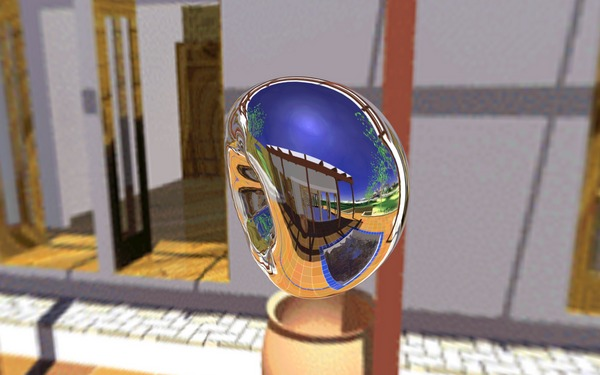
\includegraphics[width=250px]{images/graphics/bubble-reflection-effects-demo.jpg}
    \caption{The \emph{NVIDIA} bubble demo showcasing advanced reflections using cube mapping (\emph{NVIDIA} \cite{NVIDIABubble}, 2000).}
    \label{fig:bubble-reflection-demo}
\end{figure}

\noindent
Before the integration of specialized hardware, games like \emph{Wolfenstein 3D} or the 
original \emph{Doom} made heavy use of \ac{CPU} computations for graphics processing, 
executed sequentially \cite{NVIDIA1999}. A major problem was the demand for increasing 
geometrical detail. Games needed to get bigger, more photo-realistic and provide more dense 
geometry. Increasing the amount of triangles rendered, ultimately led to worse runtime 
performance. The advent of a dedicated, massively parallel chip to perform a large amount of 
operations introduced a solution for this problem. Over the years, more and more stages of the 
rendering pipeline were offloaded to the \ac{GPU}, which in turn resulted in a lot of new effects, 
games with higher triangle density and new lighting technology. As mentioned before, the \emph{NVIDIA 
GeForce 256} introduced cube mapping to the pipeline, featuring real-time reflections, which is 
shown in figure \ref{fig:bubble-reflection-demo} \cite{Battaglia2024}.


\subsection*{Rendering Pipeline} \label{subsec-rendering-pipeline}

The standardization of the graphics hardware, as pioneered by \emph{NVIDIA}, in concert with capable 
graphics \ac{API}s like \emph{Direct3D} or \emph{OpenGL} kick-started huge graphical improvements in 
games and computer graphics. The heavily parallelized transformations allowed for a lot more triangles 
in games, and the hardware accelerated lighting computations made for even more realistic lighting 
throughout the rendered scenes. One significant advantage: The \ac{GPU} could operate on a large amount 
of data while not stalling the \ac{CPU} \cite{Fenno2024}.\\

\noindent
The new rendering pipeline was to be seen in a lot of games, some of the first being \emph{Epic Games'} 
\emph{Unreal Turnament} (1999) and \emph{id Software's} \emph{Quake III Arena} (1999) \cite{UnrealTurnament, 
Quake3Arena}. \emph{Microsoft's} multimedia \ac{API} \emph{DirectX 7} added support for the new \ac{TL} 
features of \ac{GPU}s. During the following years, more and more features were added, slowly evolving the 
standard towards the "modern" rendering pipeline that is used nowadays. Between the years 1999 and 2009,
20 new minor versions of \emph{DirectX} were released \cite{WikiDirectX}. [@TODO: Check Wikipedia source] 

\begin{figure}[h]
    \centering
    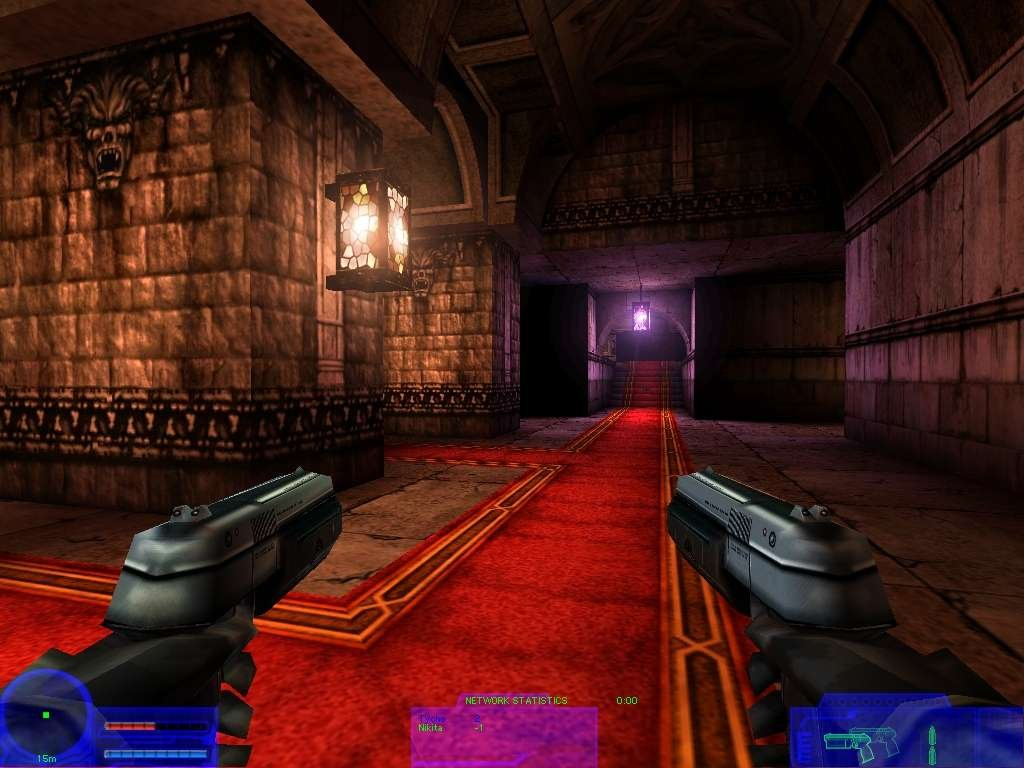
\includegraphics[width=172.5px]{images/graphics/unreal-turnament.jpg}
    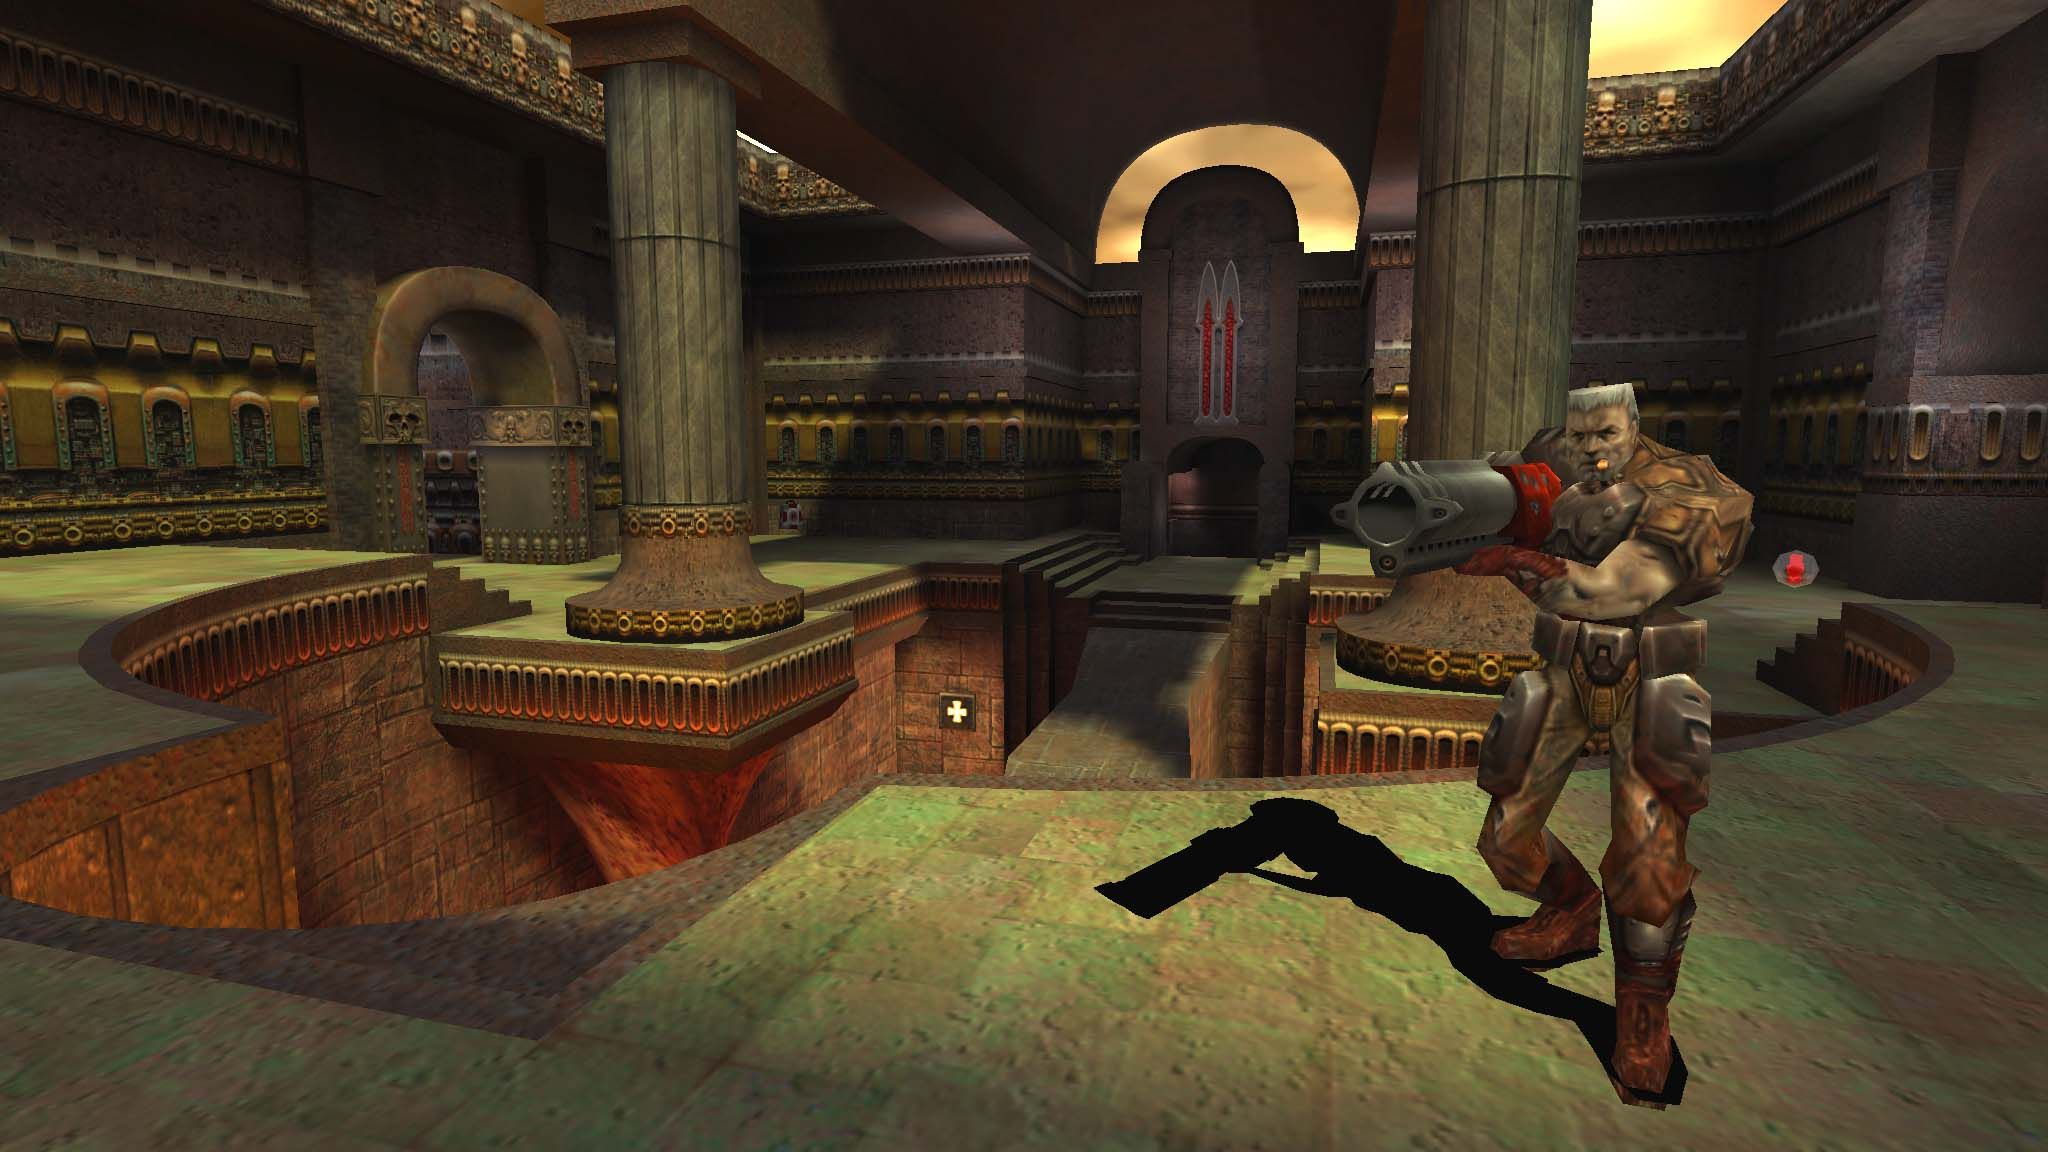
\includegraphics[width=230px]{images/graphics/quake-iii-arena.jpg}
    \caption{A screenshot from the game \emph{Unreal Turnament} (1999) (left) and \emph{Quake III Arena} (1999) 
    (right) \cite{GamespotUnrealTurnament, GameWatcher2006}.}
    \label{fig:unreal-turnament-quake-arena}
\end{figure}


\subsection*{Deferred Rendering} \label{subsec-deferred-rendering}

[@TODO: Sources]
With a lot of innovative hard and software, the games got complexer and real-time computer graphics got even more 
photo-realistic. The demand for more light sources increased in an attempt to make game worlds more realistic. 
However, more light sources posed some problems for the developers. When using the traditional rendering pipeline,
lighting is calculated on a per-vertex basis. Interpolation can be used to generate lighting results for every sample 
in between the vertices. Still, every vertex must be considered in combination with all light sources. This creates a 
dependancy between the amount of vertices and the amount of lightsources. Basically, adding a few more light sources 
will drastically increase computatoin times of the final image. Another method can be adopted: \emph{Deferred Shading}.
It was first adopted for the use on \ac{GPU}s by Dean Calver \cite{Calver2004} in 2004. This technique makes use of 
multiple render targets, and writes the data necessary for the lighting calculations into various buffers. This way, 
the surface normals, the specular intensity, the albedo (texture color), the depth and more values can all be stored 
individually, as per-pixel data. This includes the relevant data for the lighting calculations. When all buffers are 
drawn, the final result is easily found by looking up all the relevant data from each buffer at one pixel coordinate 
and combining them to a final result. Figure \ref{fig:deferred-shading-buffers} shows all the buffers used for the 
creation of one frame in \emph{Guerilla Games'} \emph{Killzone 2} (2007) \cite{KillzoneFandom}. 

\begin{figure}[h]
    \centering
    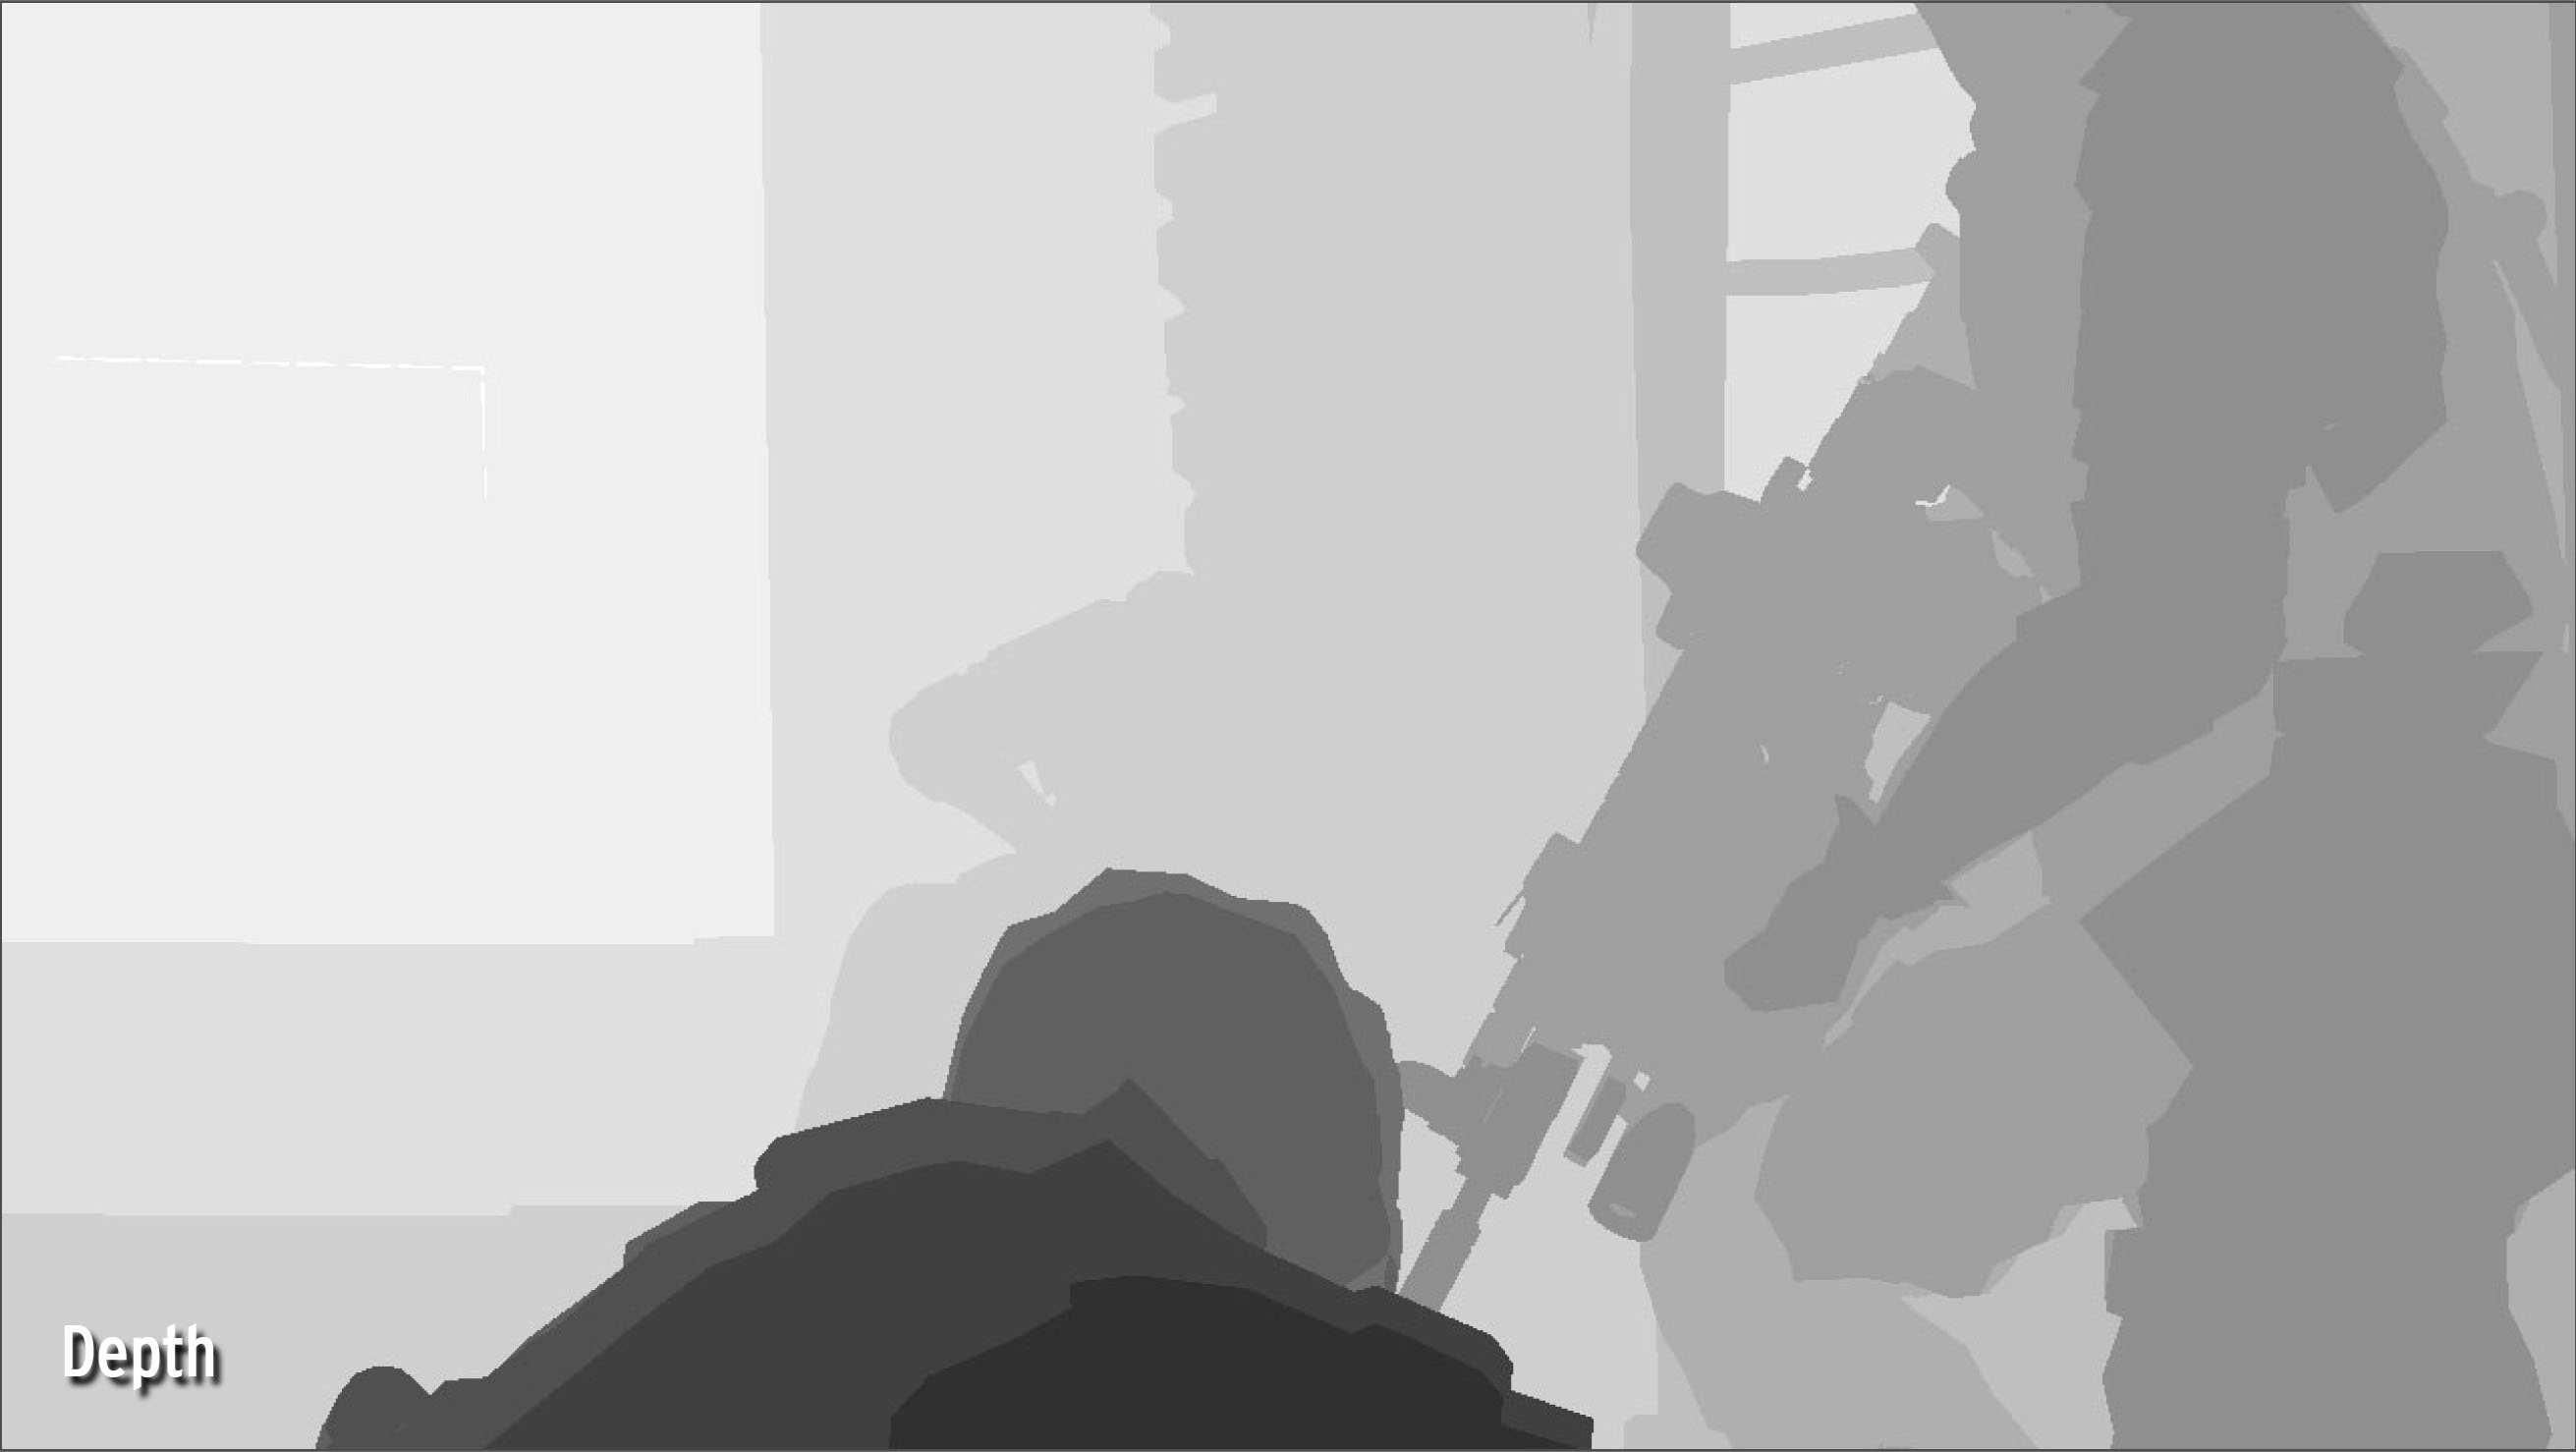
\includegraphics[width=175px]{images/graphics/killzone-2-buffer-depth.jpg}
    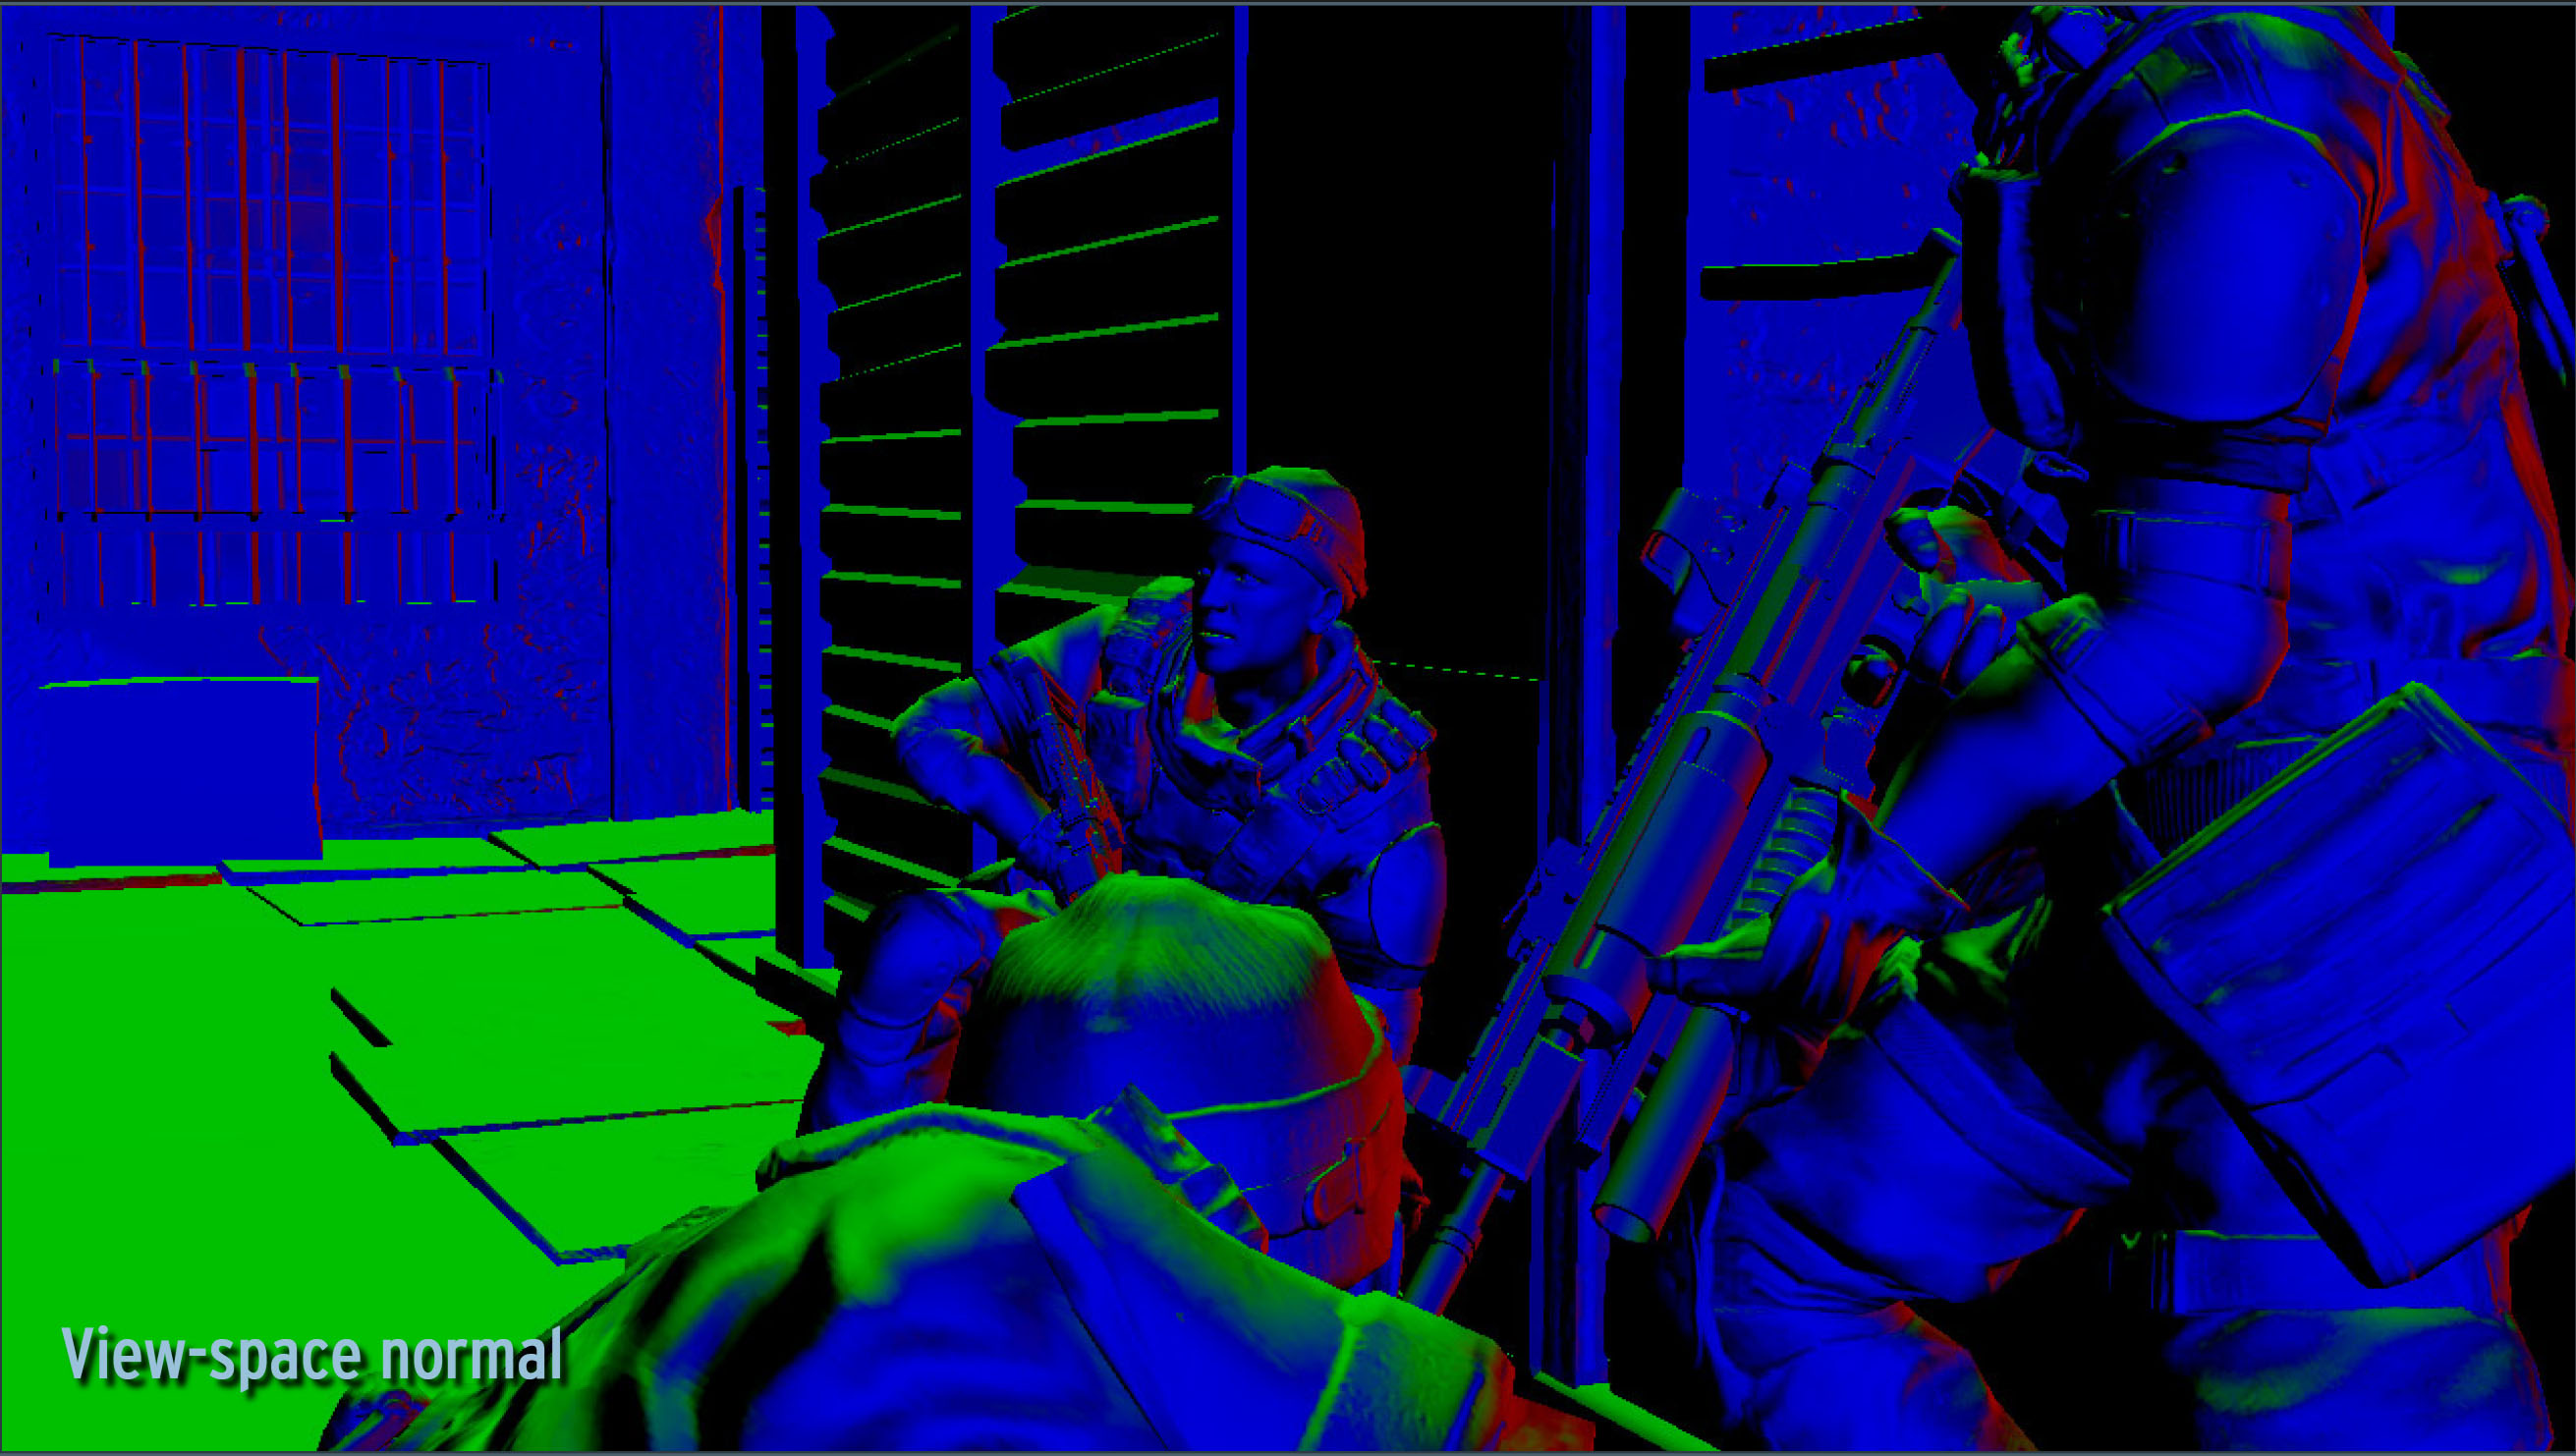
\includegraphics[width=175px]{images/graphics/killzone-2-buffer-vsn.jpg}
    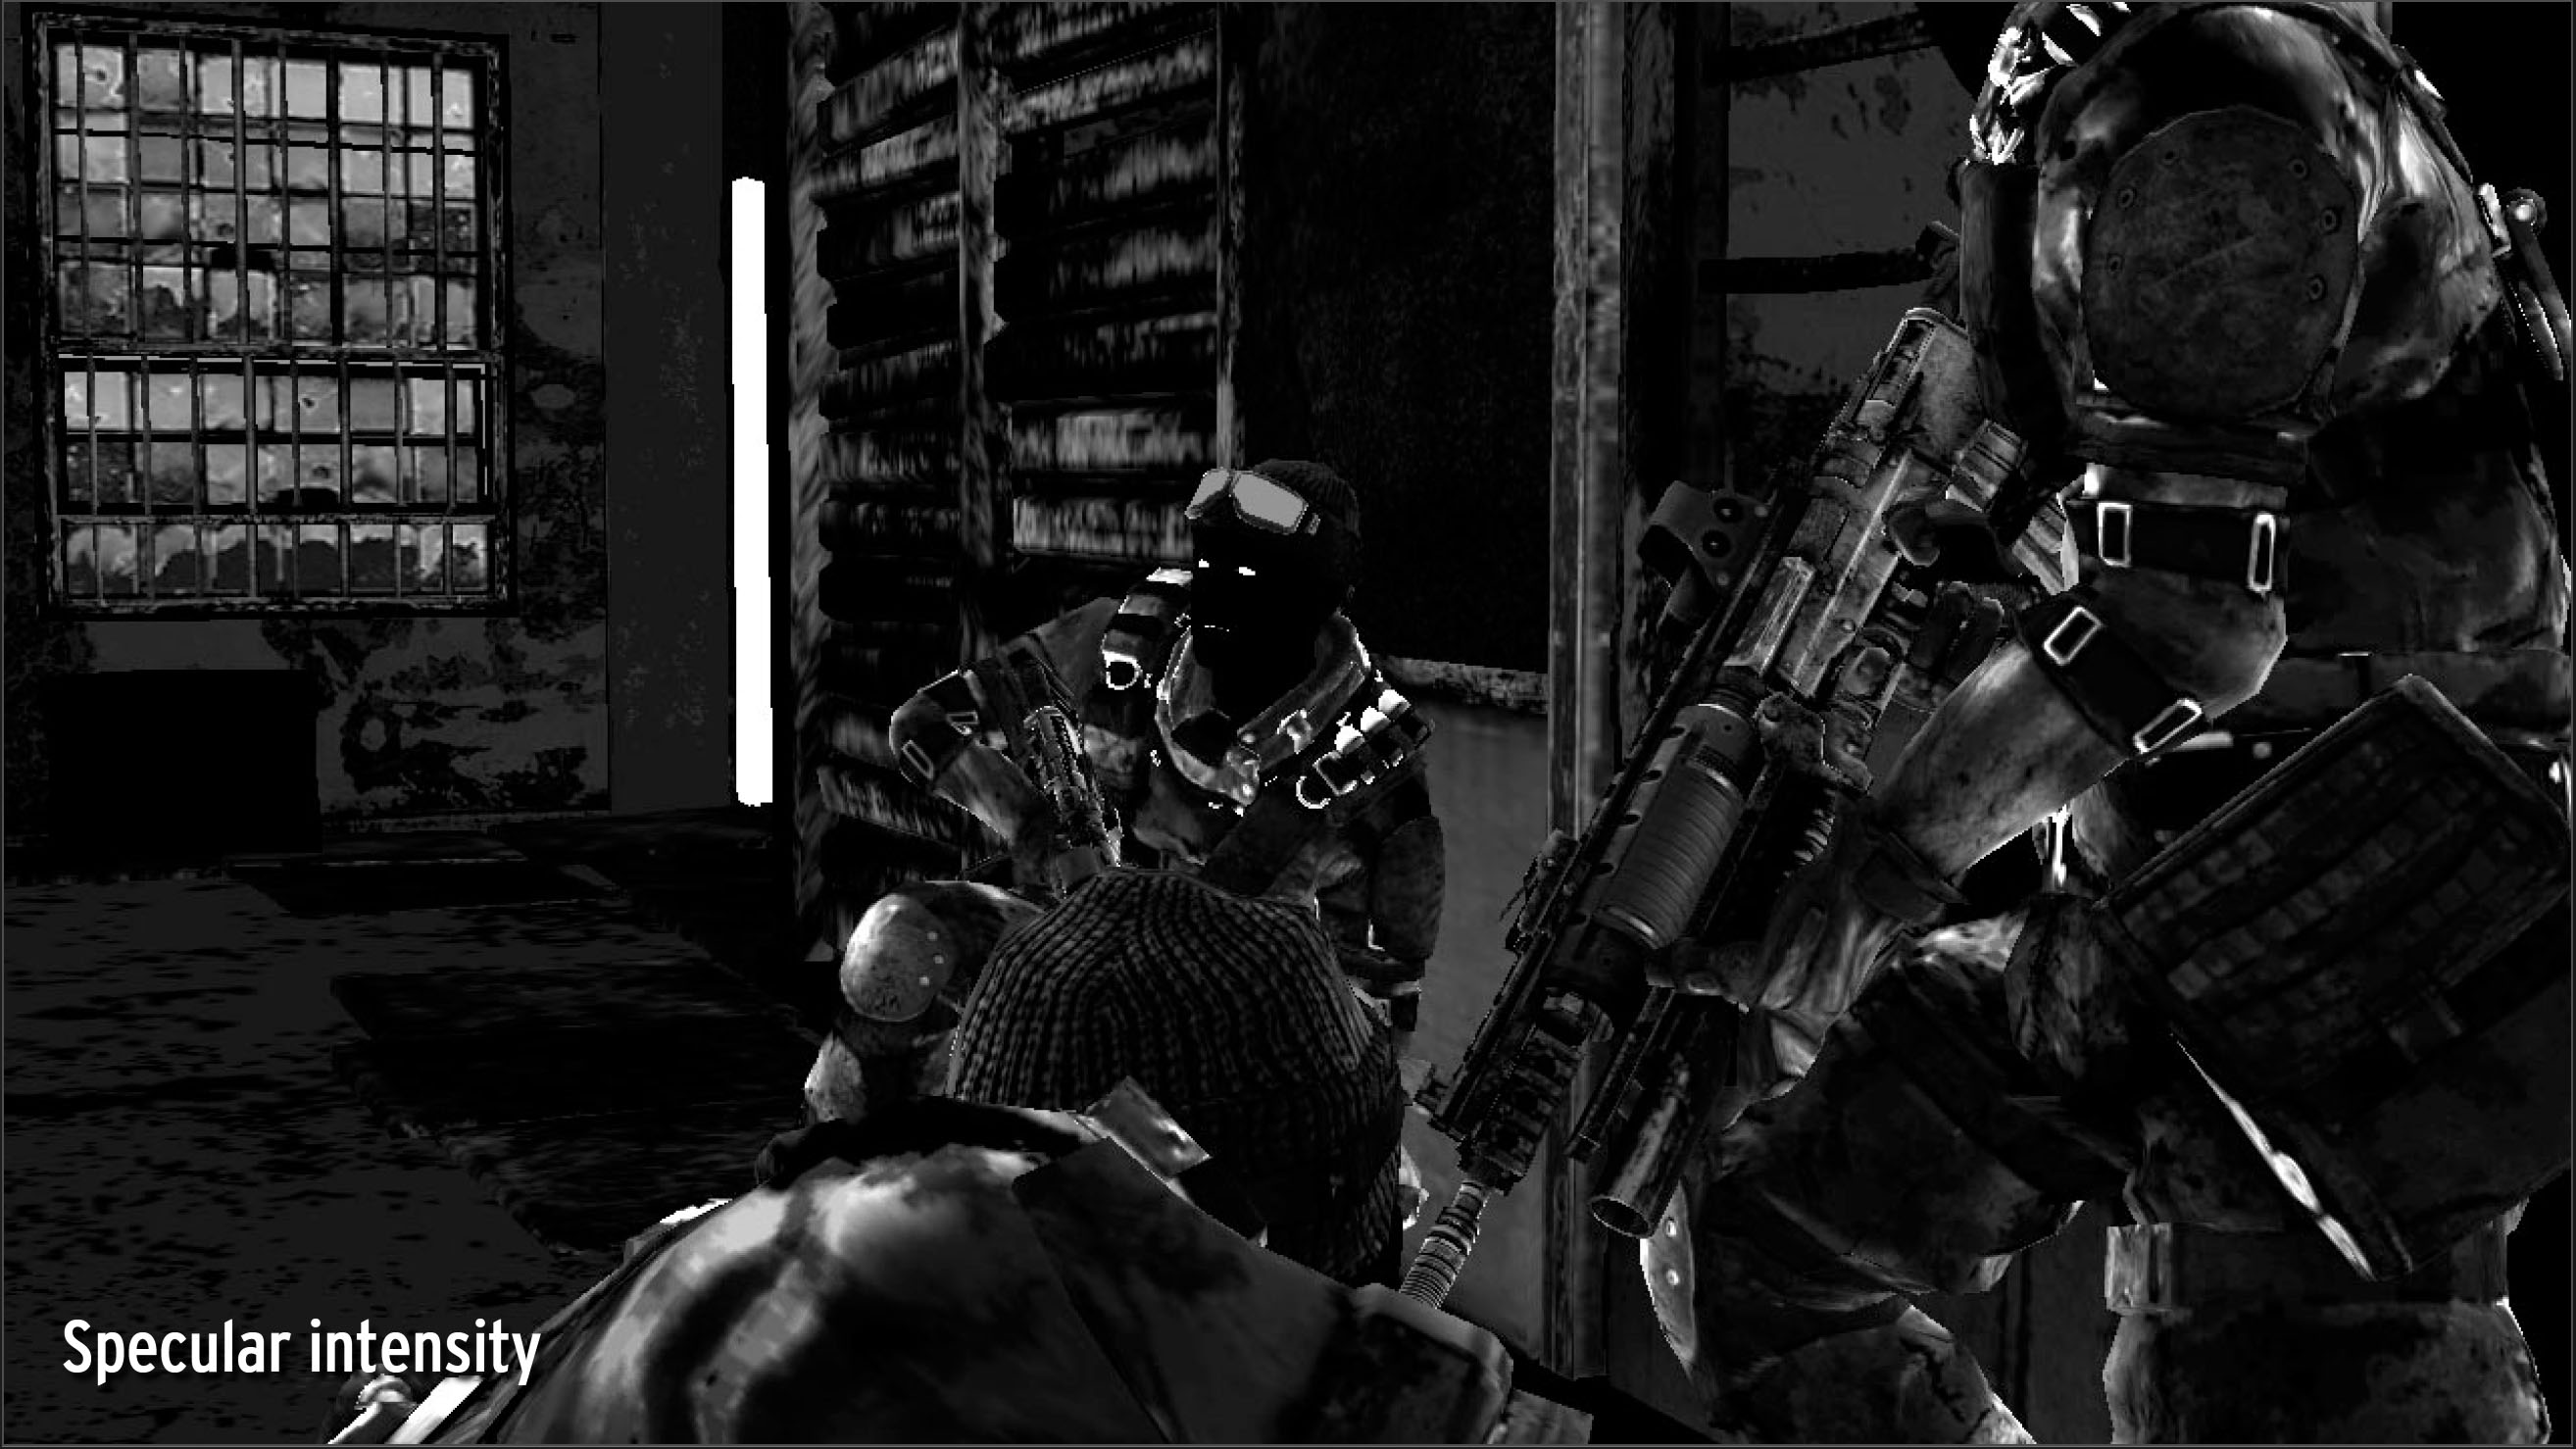
\includegraphics[width=175px]{images/graphics/killzone-2-buffer-specular.jpg}
    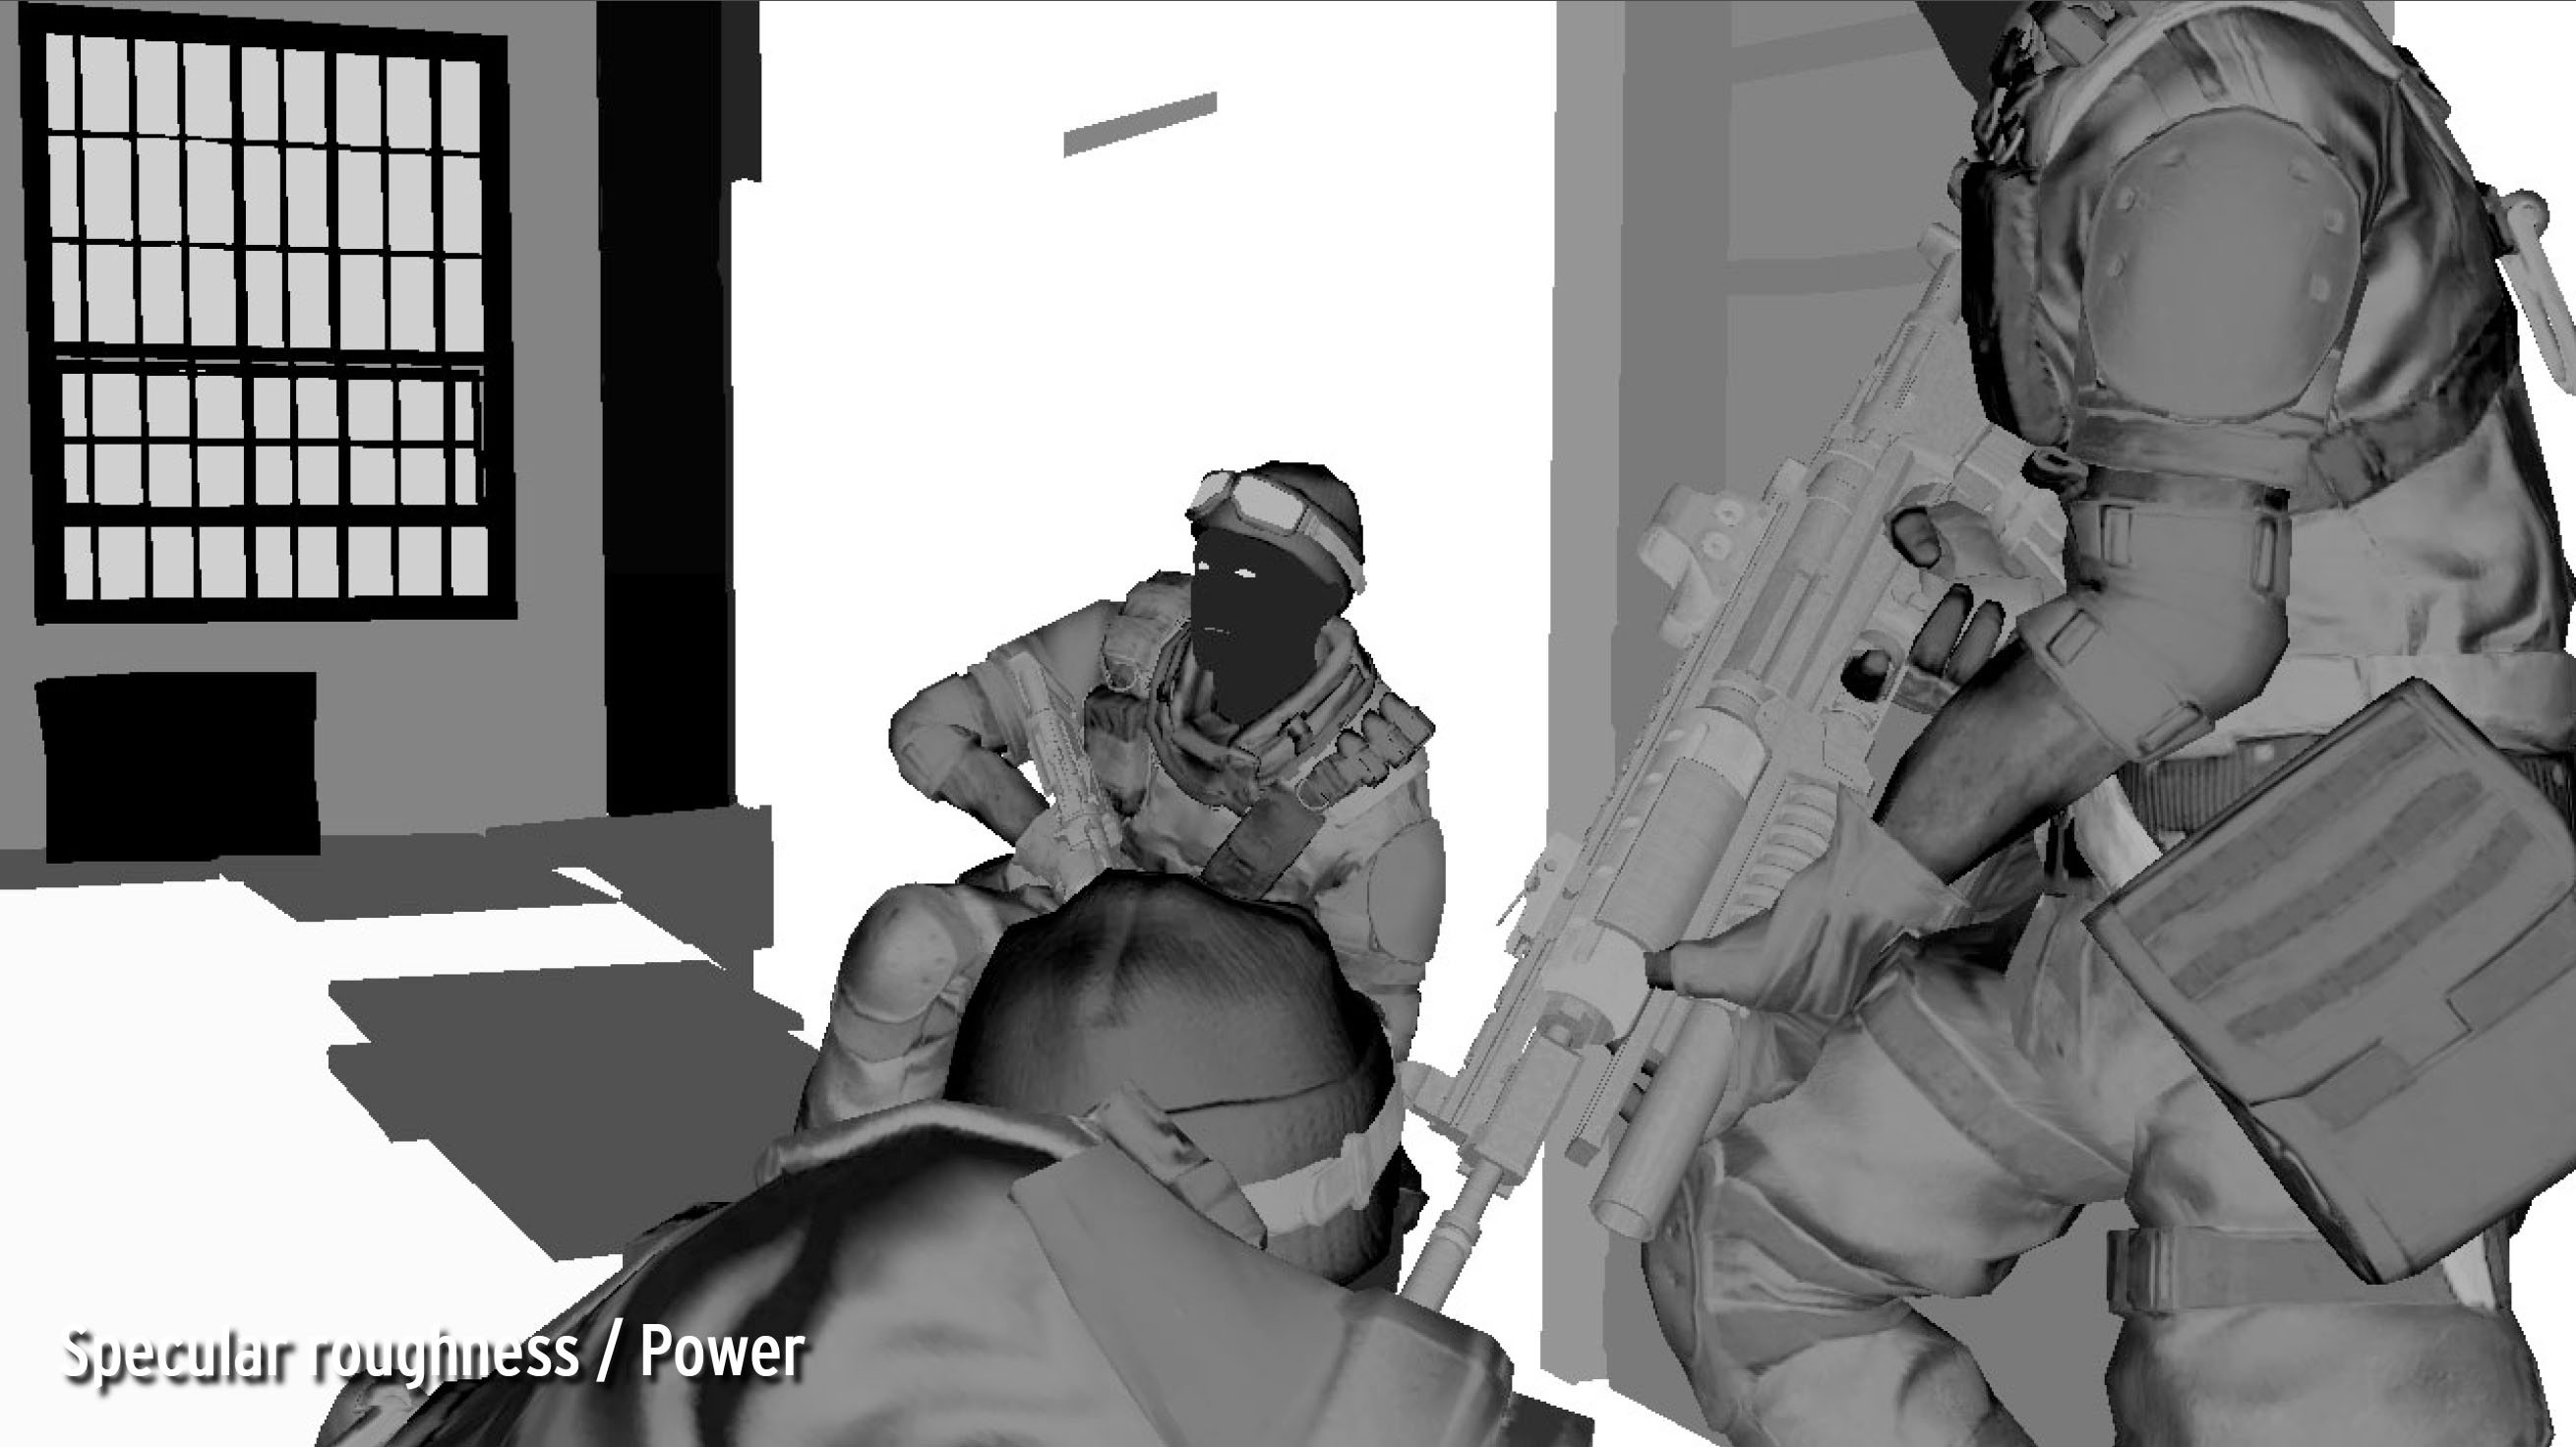
\includegraphics[width=175px]{images/graphics/killzone-2-buffer-specular-rough.jpg}
    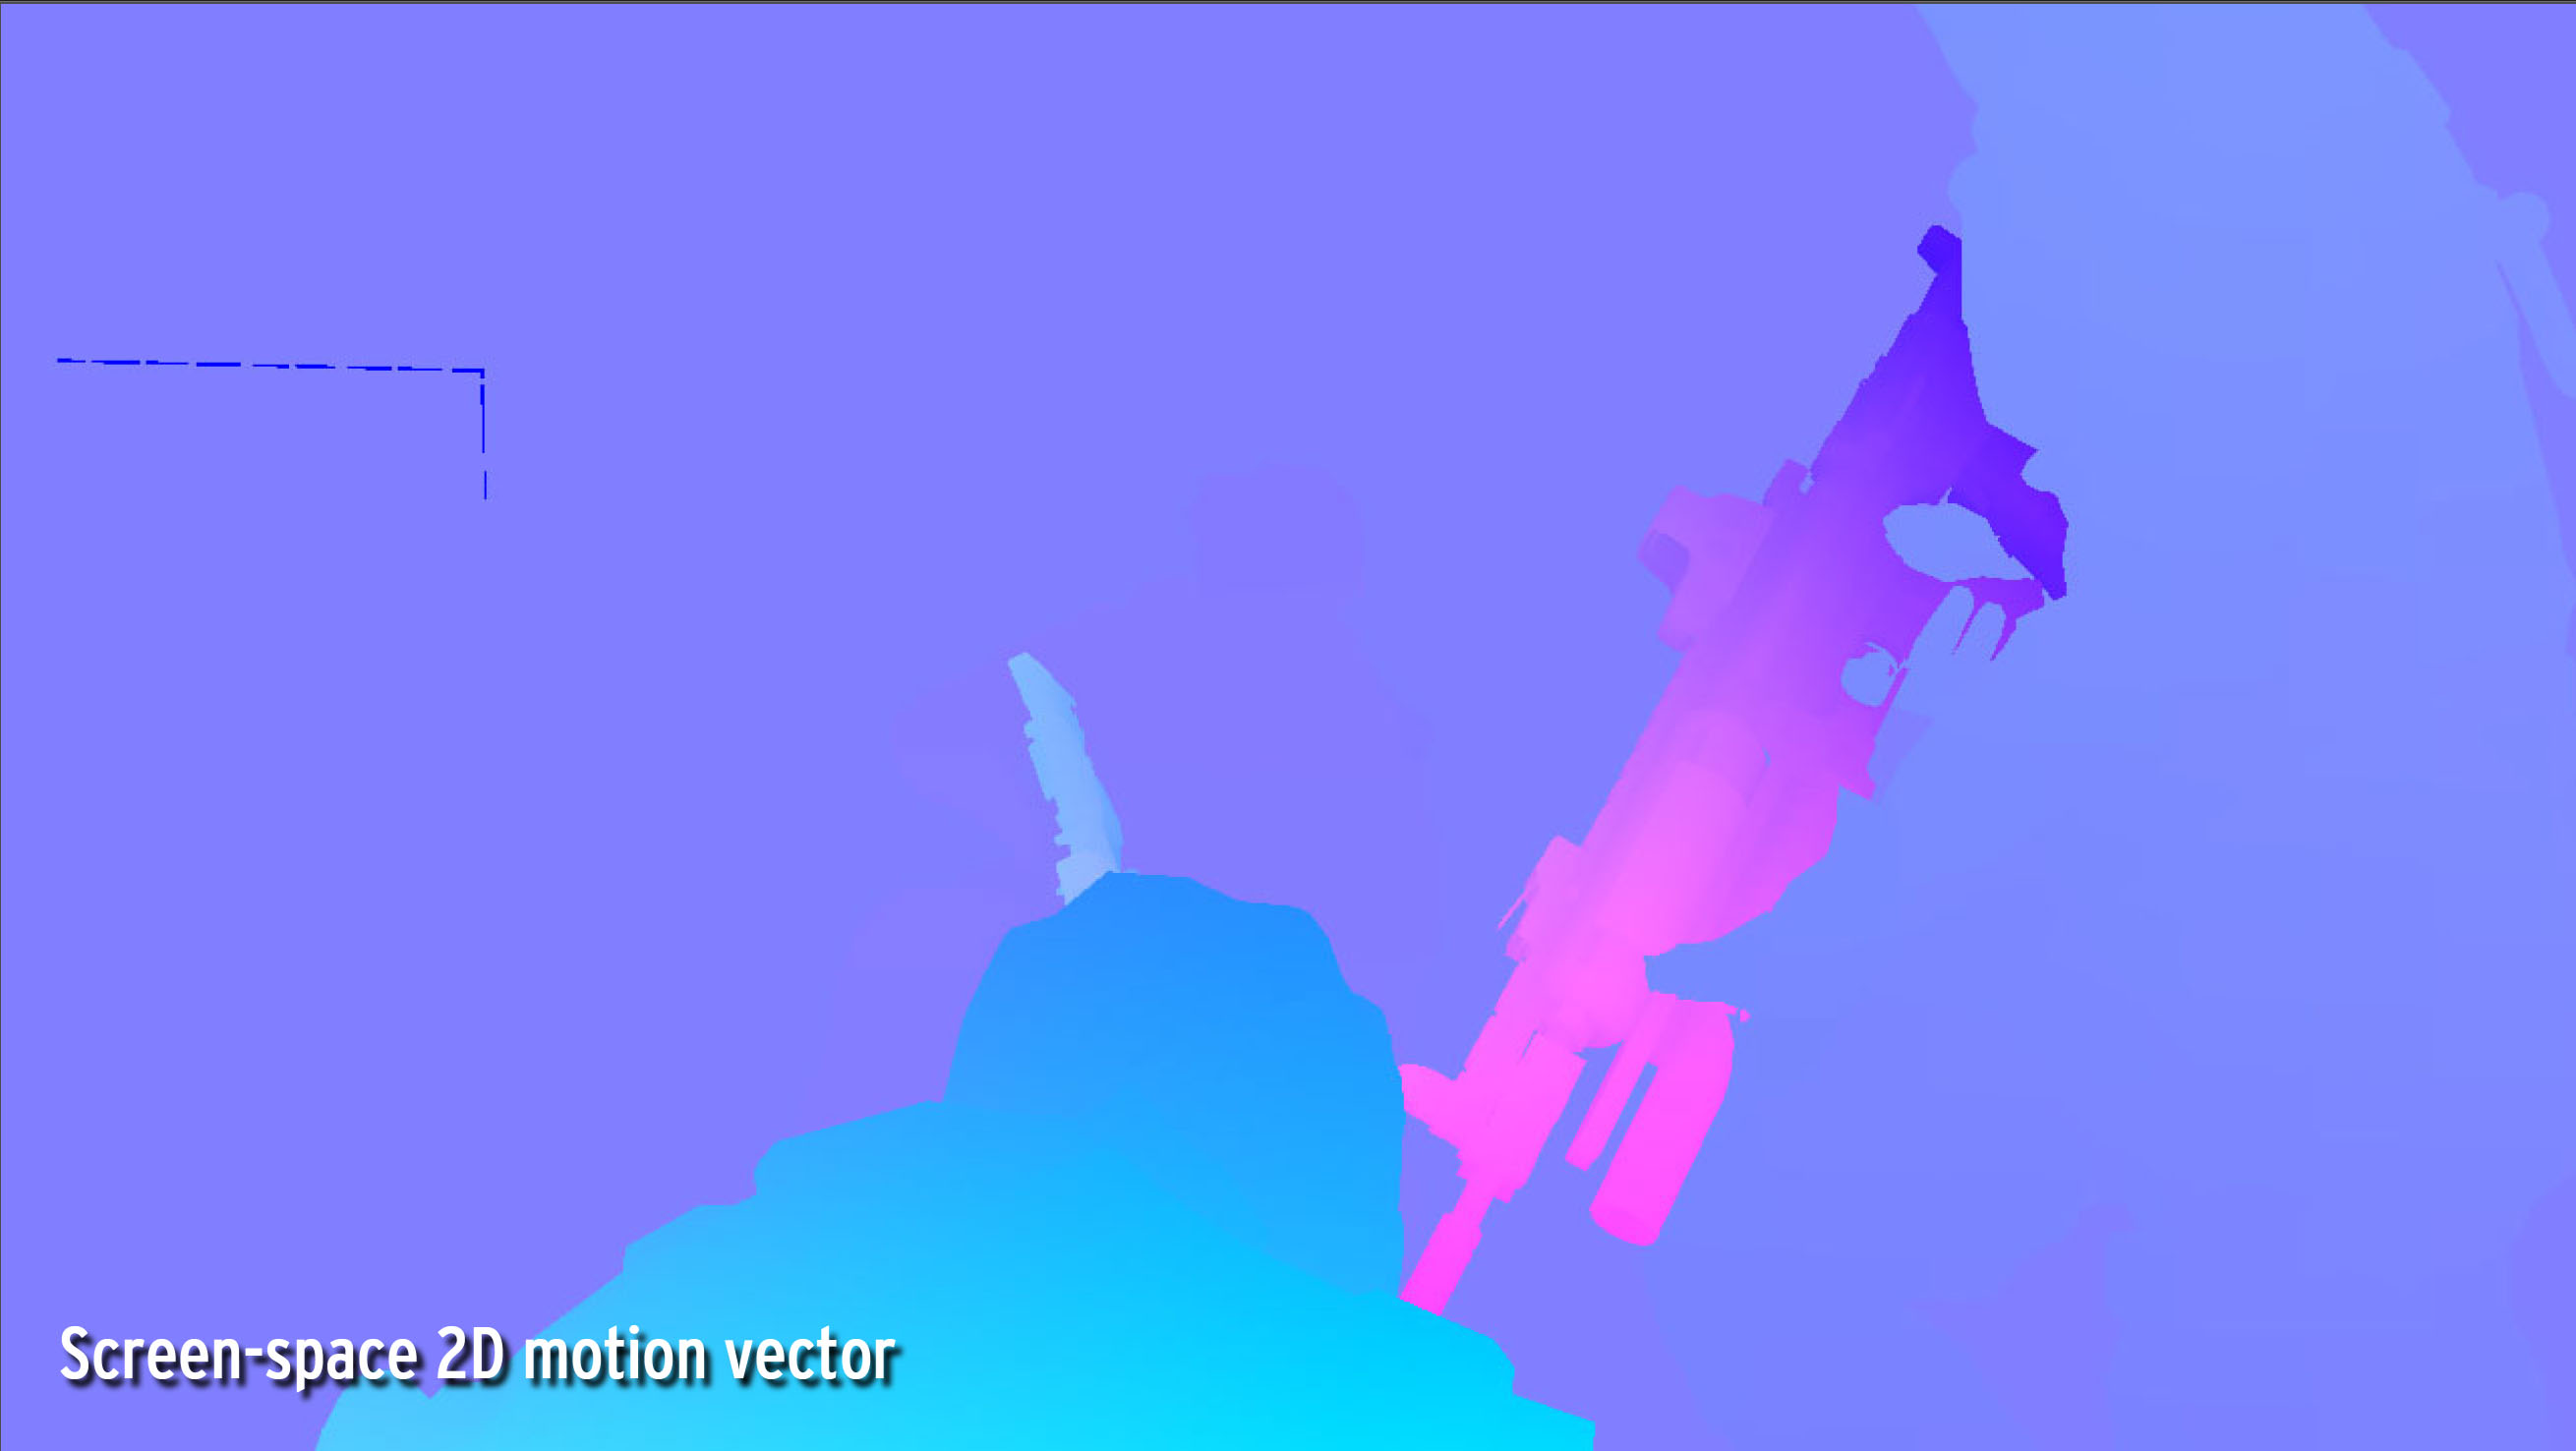
\includegraphics[width=175px]{images/graphics/killzone-2-buffer-ss-motion.jpg}
    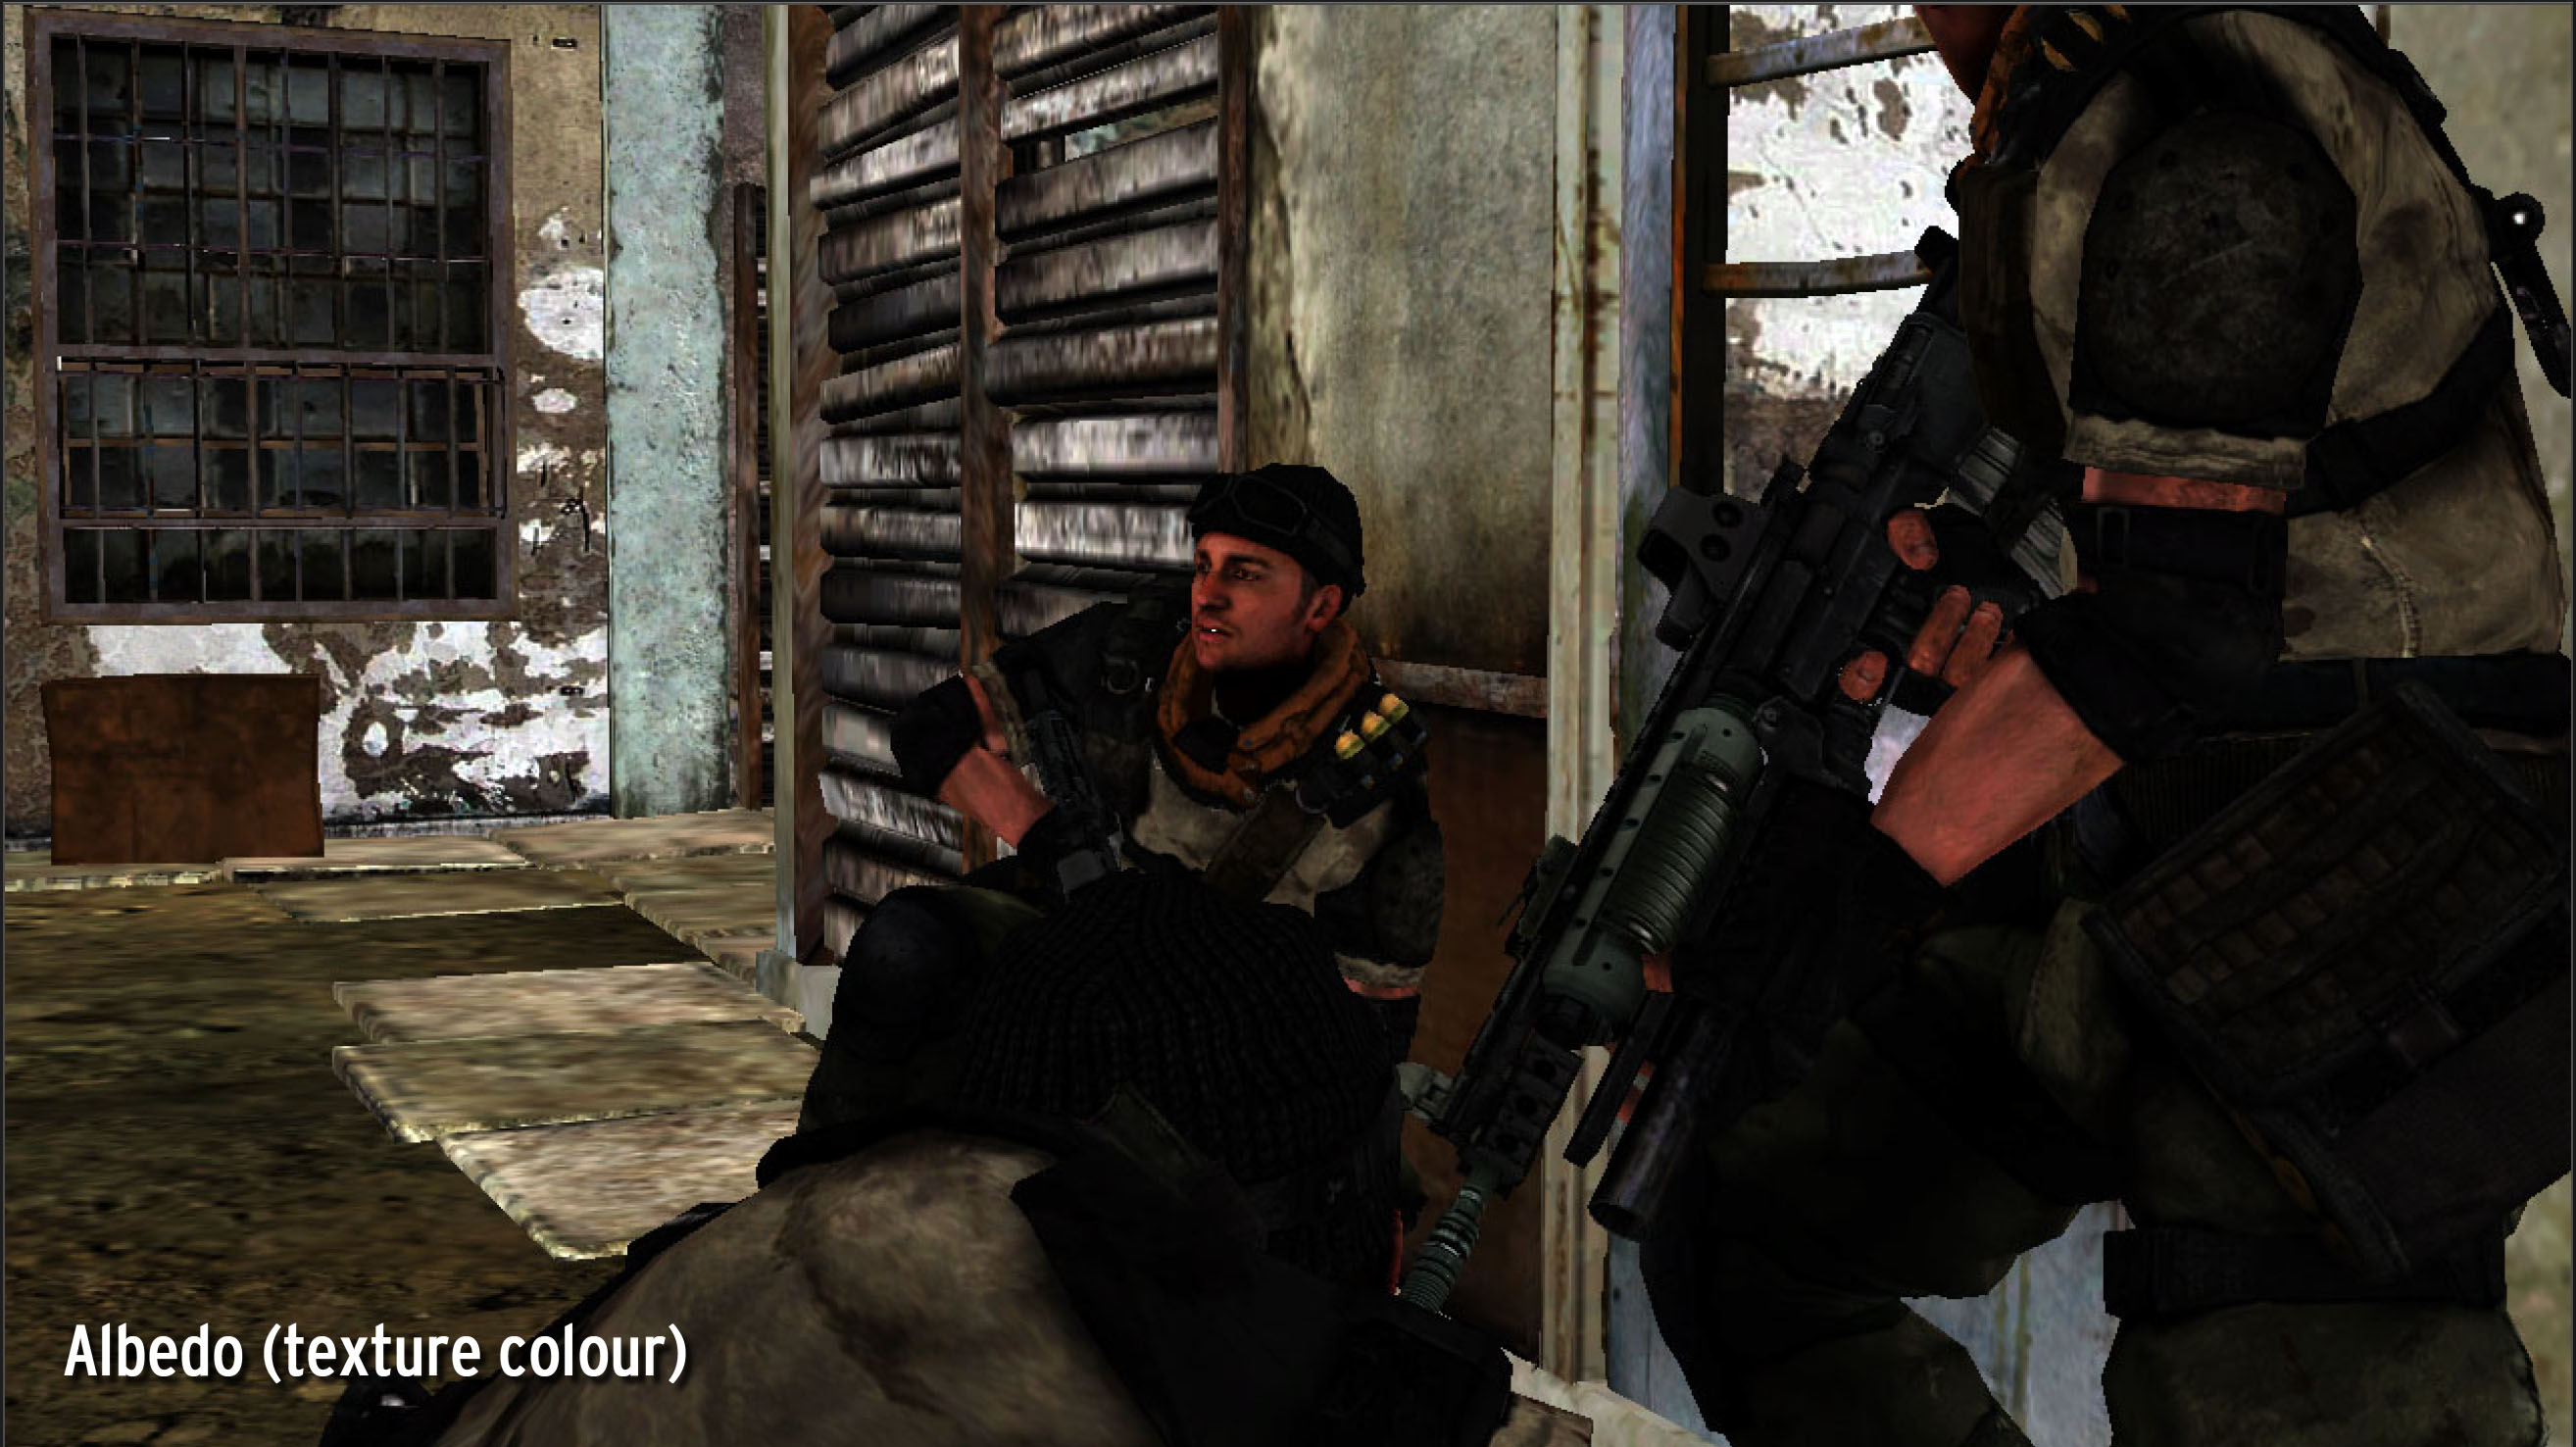
\includegraphics[width=175px]{images/graphics/killzone-2-buffer-albedo.jpg}
    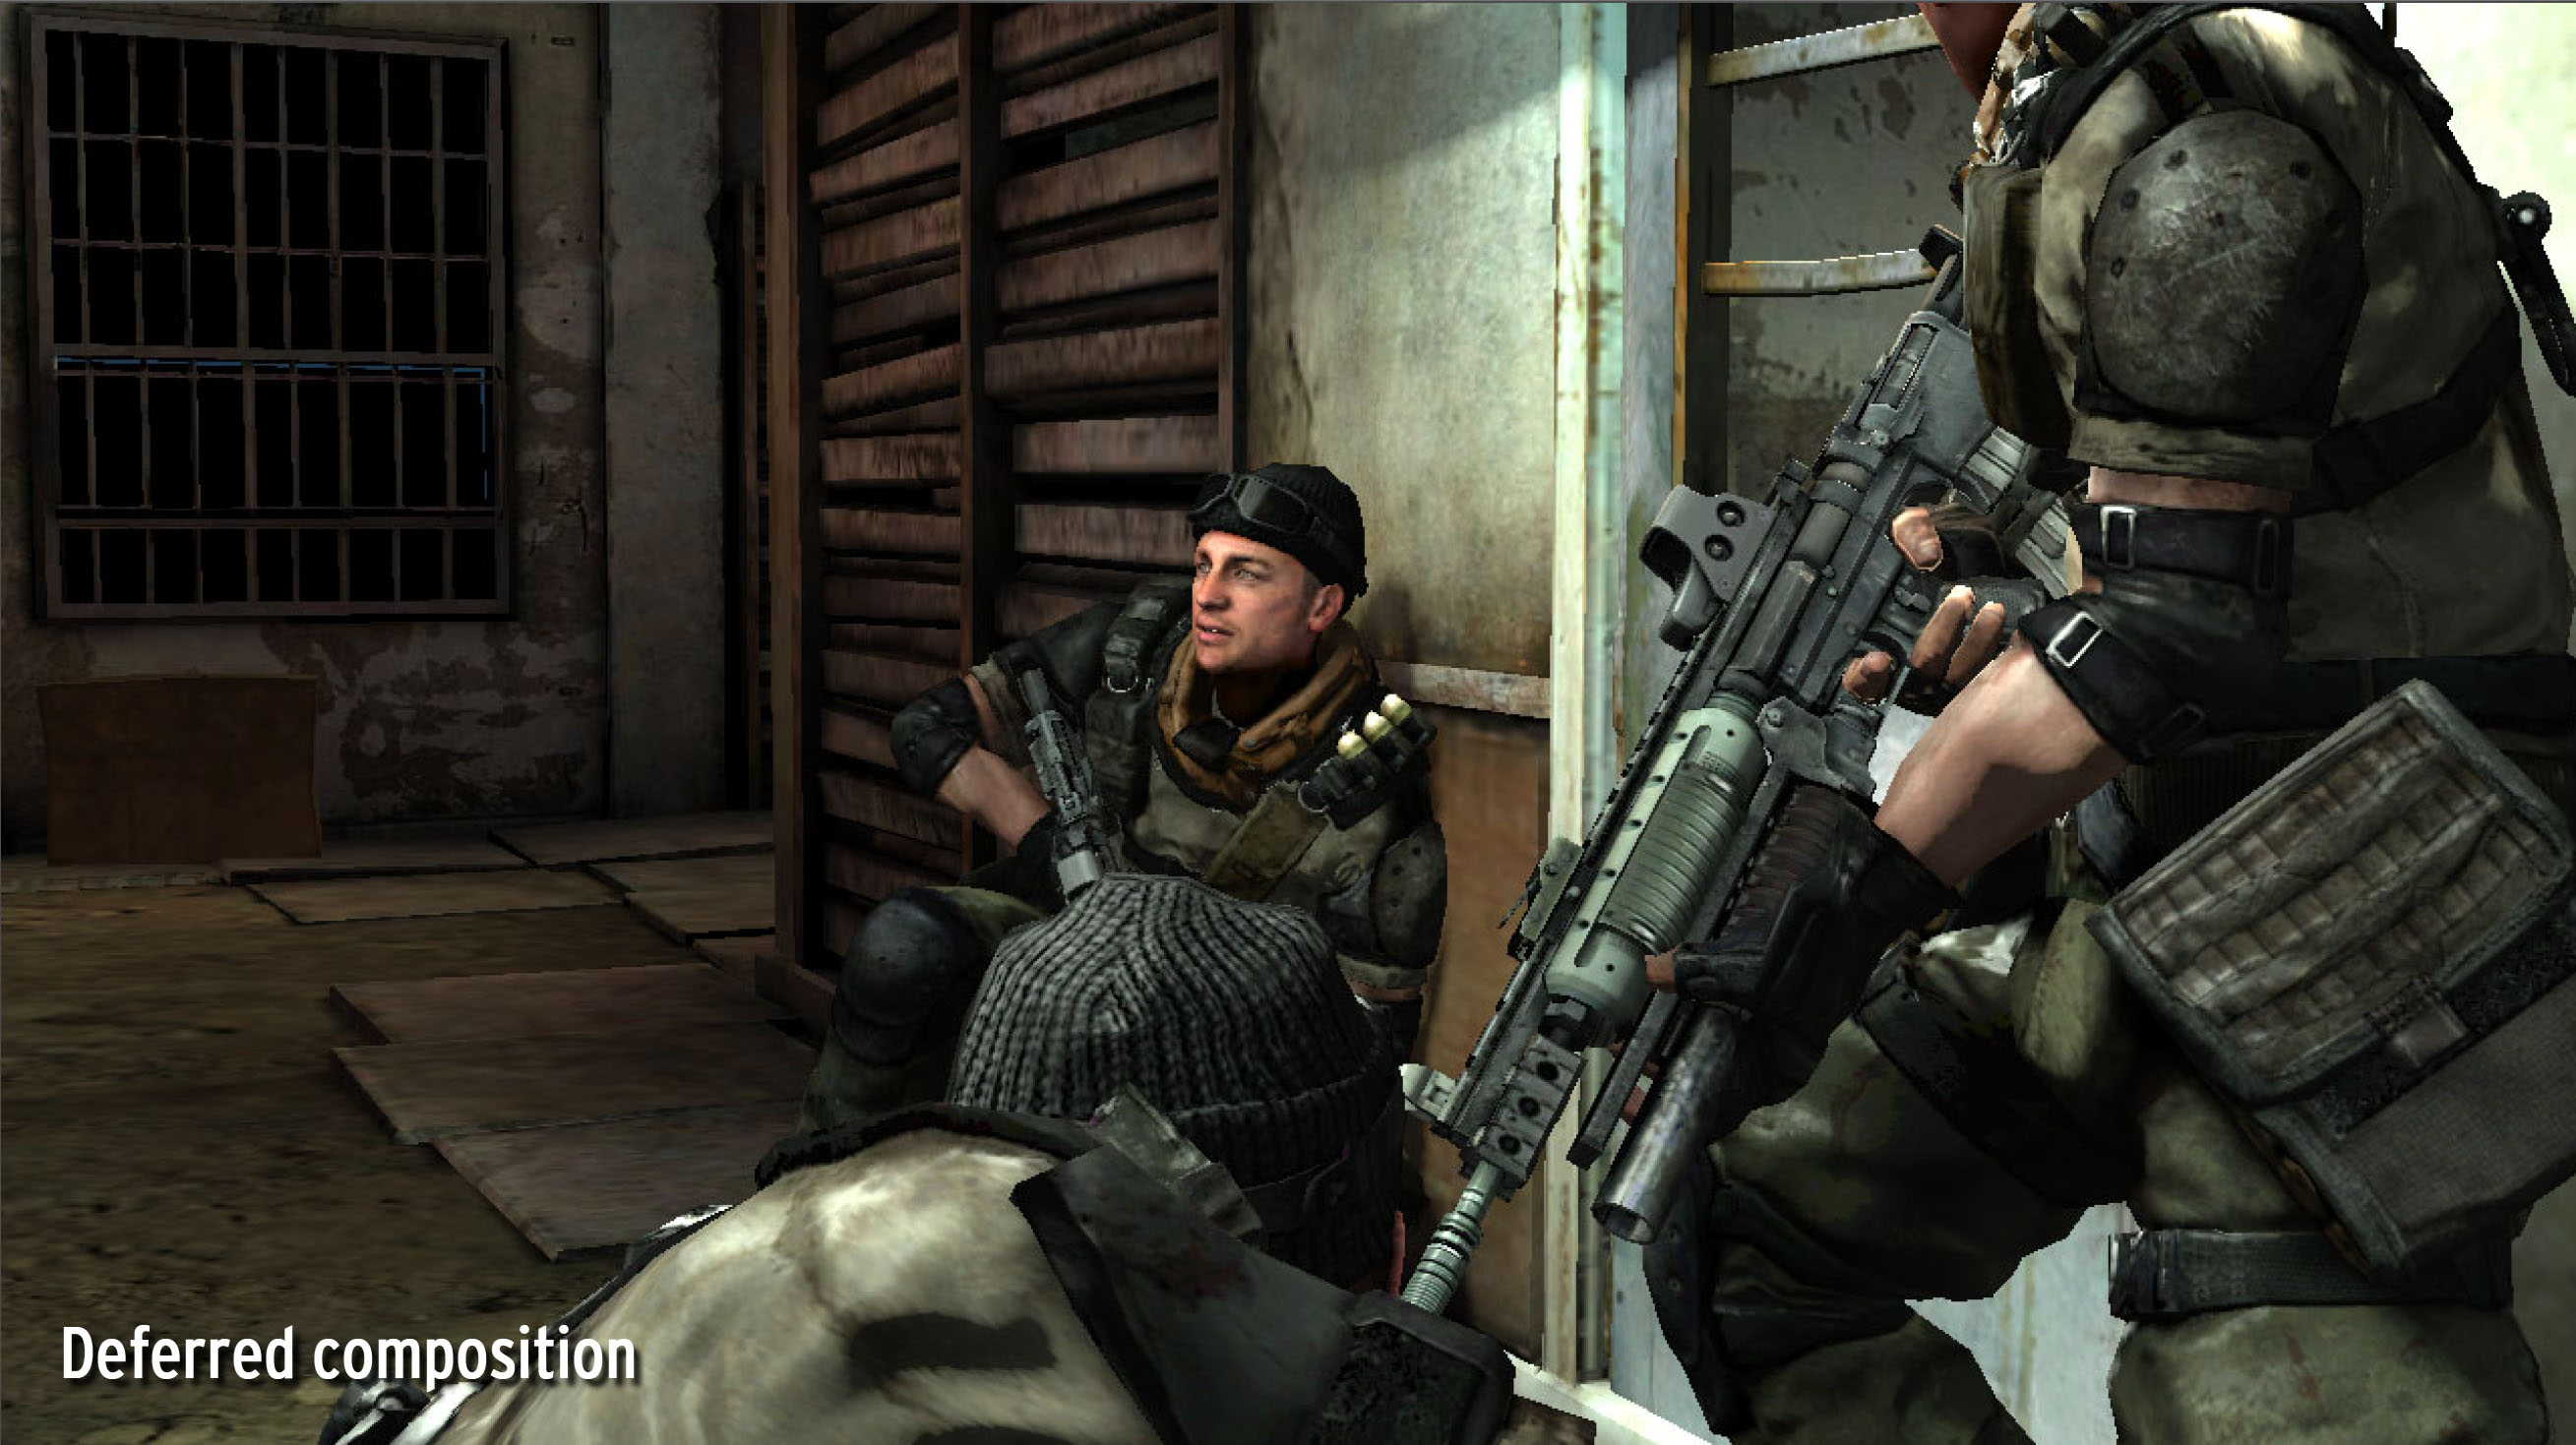
\includegraphics[width=175px]{images/graphics/killzone-2-buffer-composed-result.jpg}
    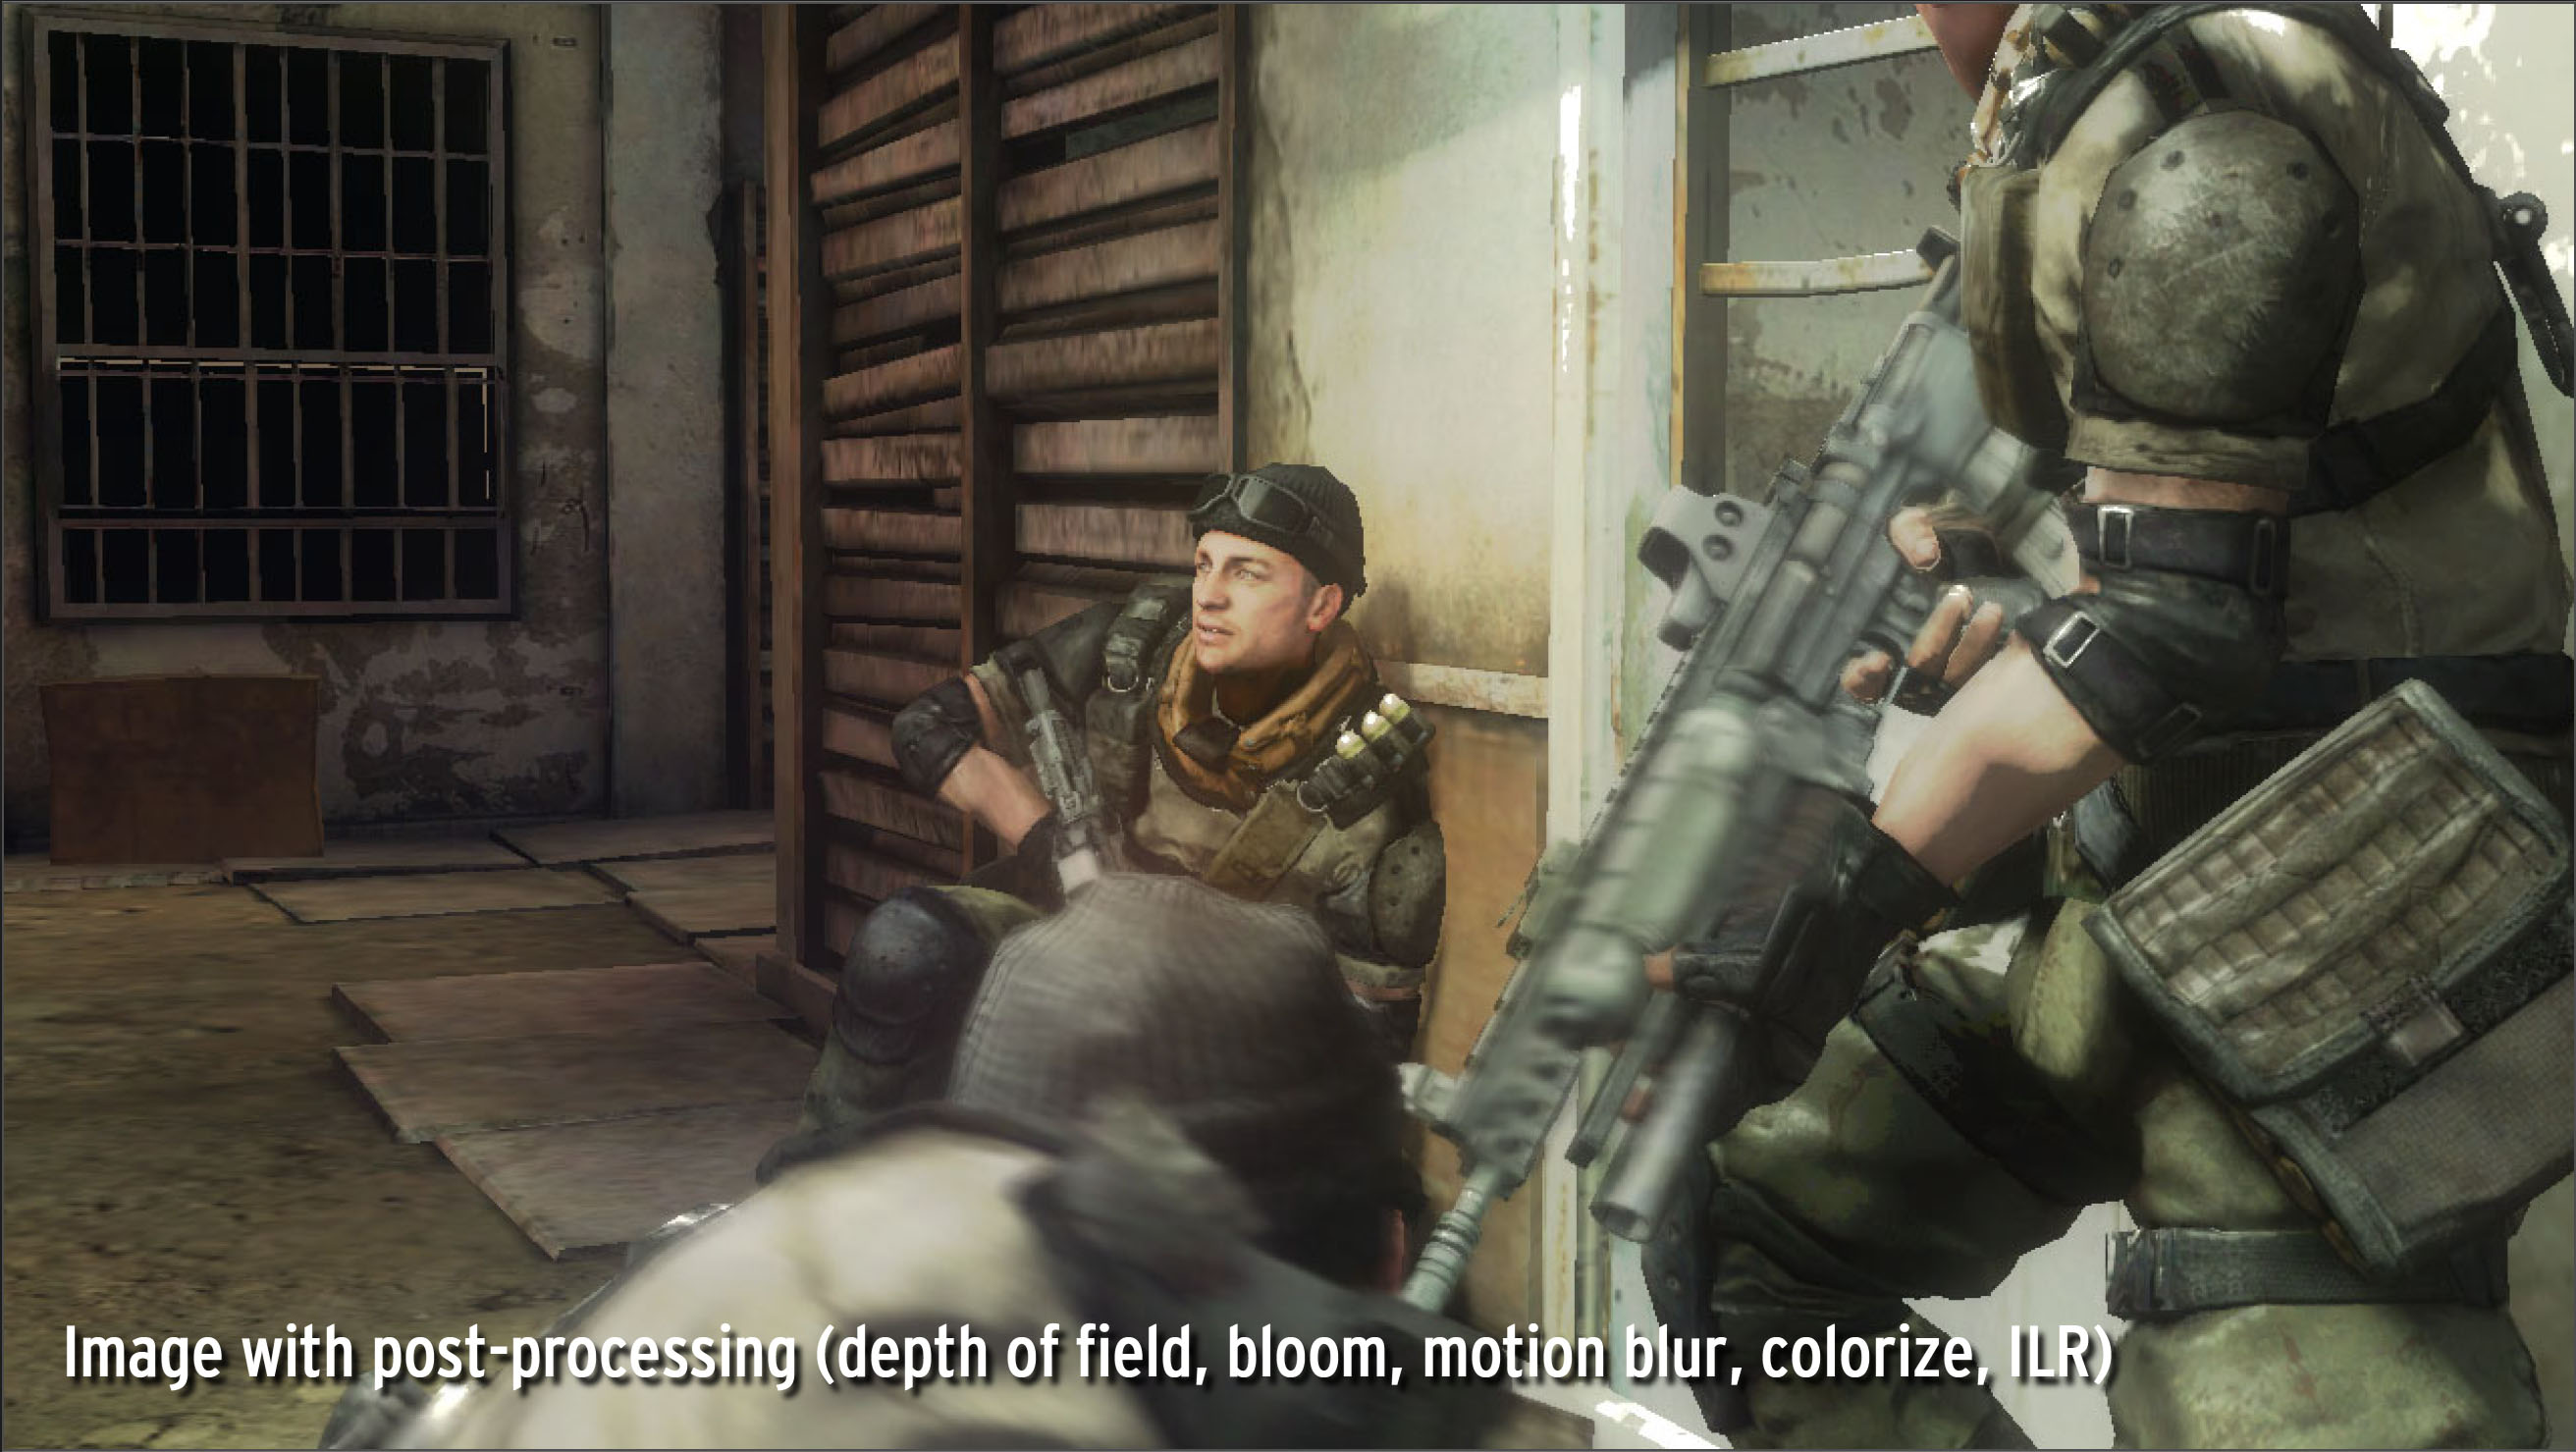
\includegraphics[width=175px]{images/graphics/killzone-2-buffer-post.jpg}
    \caption{Different buffers for \emph{Deferred Shading} in \emph{Guerilla Games'} \emph{Killzone 2} (2009) 
    \cite{Valient2007}.}
    \label{fig:deferred-shading-buffers}
\end{figure}

\noindent
As Akenine-Möller et al. point out, "the contribution of the models’ geometry has been fully decoupled from lighting 
computations" \cite{AkenineMoeller2018}. \emph{Deferred Shading} encompasses a lot more optimizations, like compression, 
light clustering, deferred texturing and more \cite{AkenineMoeller2018}. All these techniques combined can ultimately 
result in a more efficient shading model for specific use cases, for instance, when using a lot of lights in combination 
with high density geometry.\\

\noindent
The basic idea of \emph{Deferred Shading} influenced the next couple of years of real-time graphics technology and is 
still used today for state-of-the-art game development. Dispatching work for the \ac{GPU} to operate on and optimizing 
memory and data layouts for most efficient computation has also resulted in one of the latest trends in real-time 
rendering.

\subsection*{GPU Driven Rendering}

\begin{figure}[h]
    \centering
    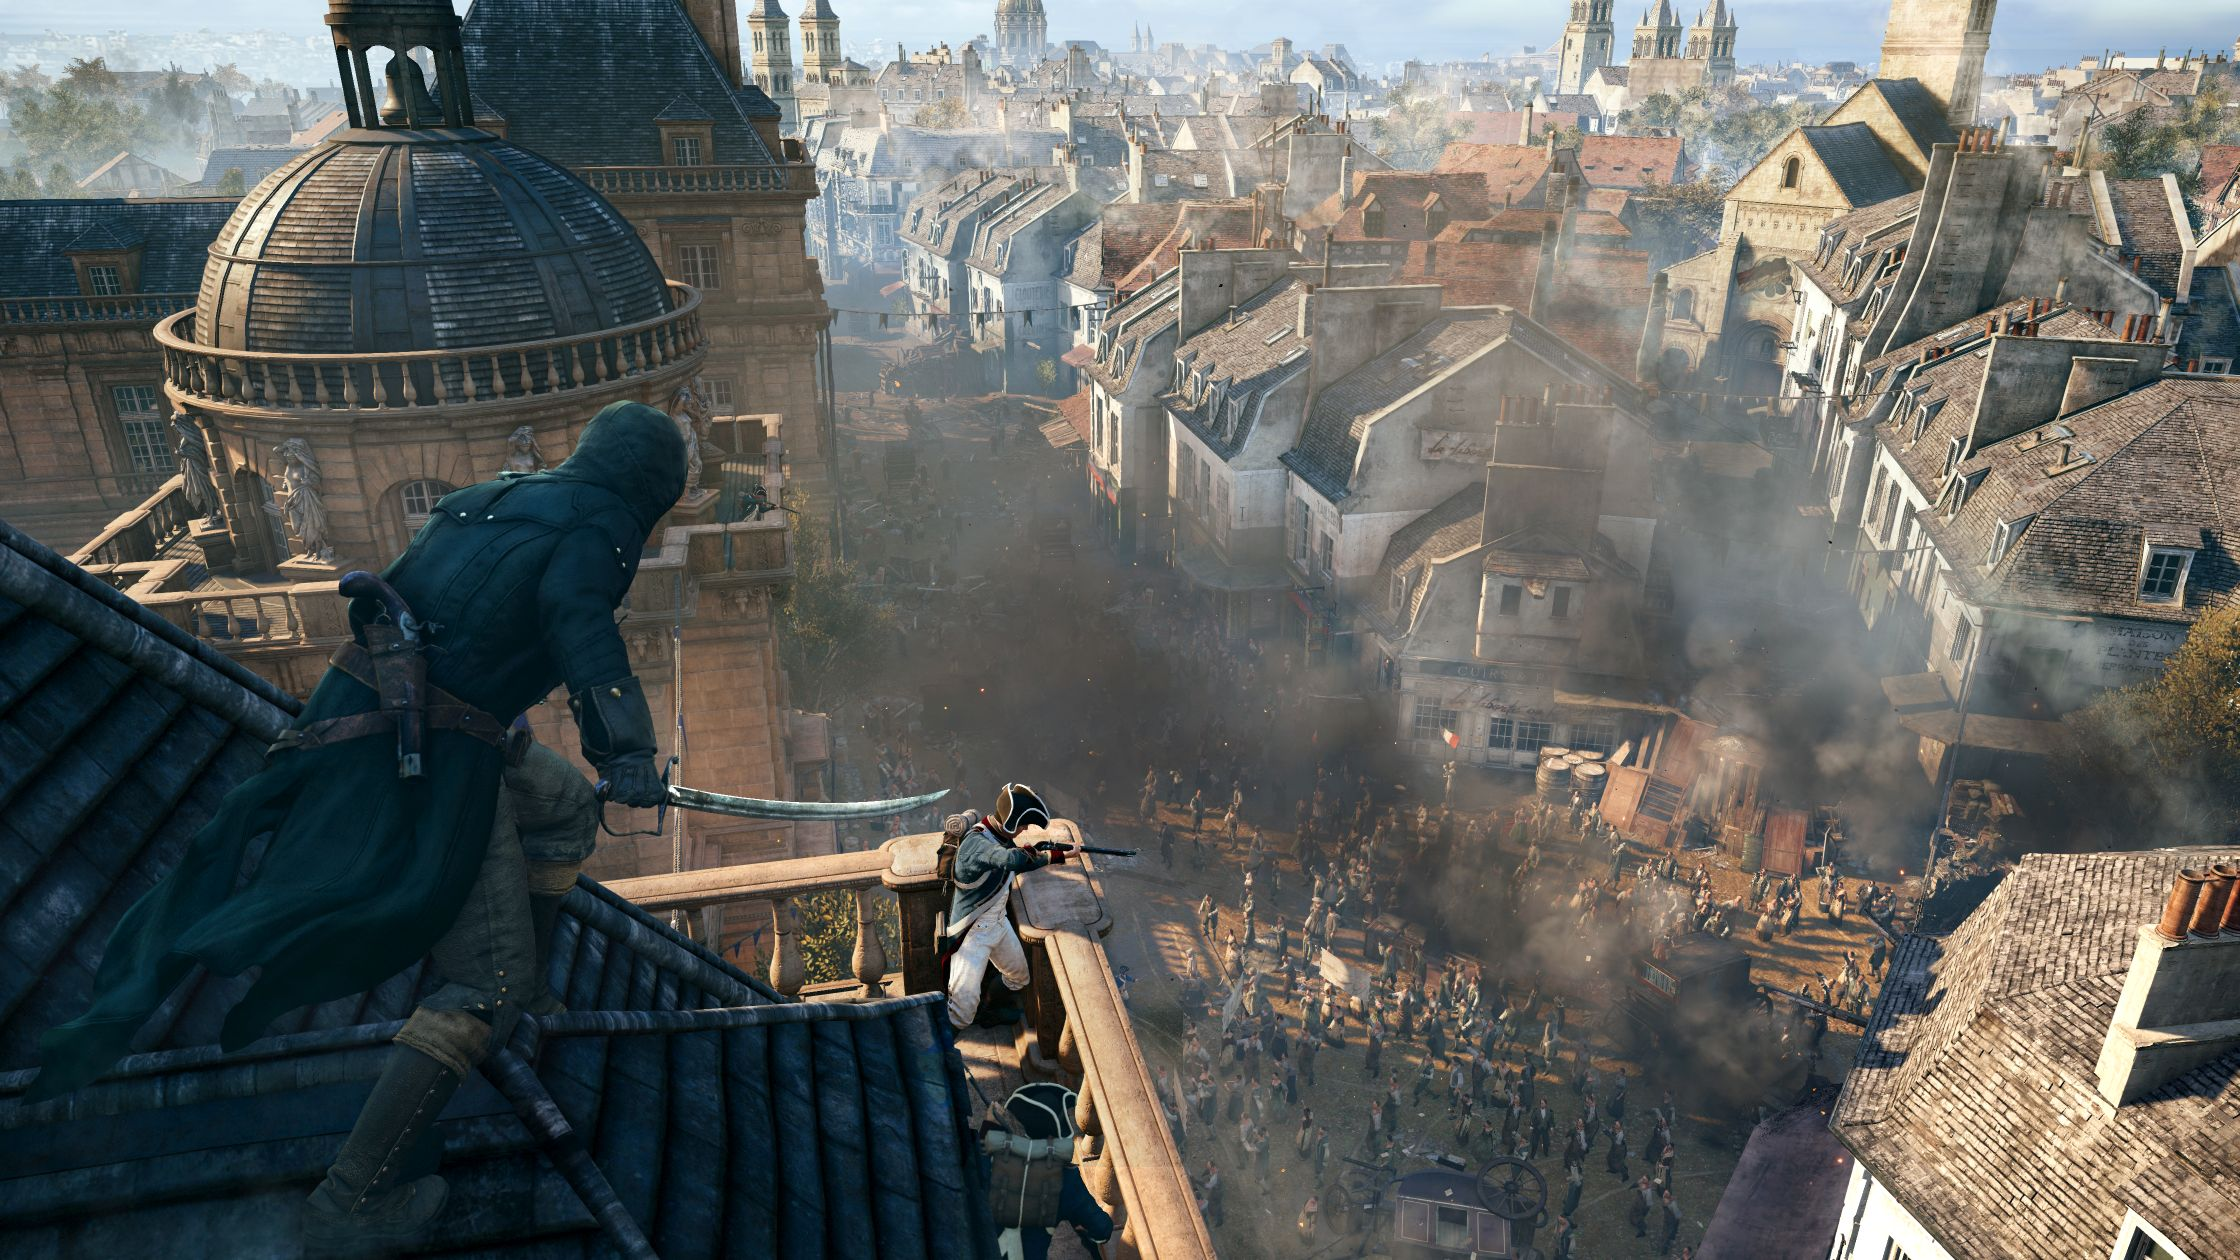
\includegraphics[width=300px]{images/graphics/assassins-creed-unity-gameplay.jpg}
    \caption{A screenshot of the game \emph{Assassin's Creed Unity} (\emph{Ubisoft} \cite{Ubisoft2014}, 2014) 
    showcasing the high density of geometry and far draw distances \cite{Burke2014}.}
    \label{fig:assassins-creed-unity-gameplay}
\end{figure}

\noindent [@TODO: Sources]
Over a decade after the first \ac{GPU} was introduced, hardware acceleration was the de facto standard in 
computer graphics and the rendering pipeline got more and more loaded with features, innovations and data. 
This led to a new bottleneck: The memory bandwith between the \ac{CPU} and \ac{GPU}. Soon, a new trend was 
developed: \emph{\ac{GPUDR}}. The goal of \ac{GPUDR} is, to minimize bandwidth between \ac{CPU} and \ac{GPU}. 
An ideal \ac{GPU} driven application would only update the camera related data (view and projection matrices) 
within a frame. Everything else would be computed by the \ac{GPU}. This trend arised with the rise of the 
\ac{GPGPU} and the better support for the more generalized \emph{compute shaders}. The defintion for when 
applications are \ac{GPU} driven and when not, is blurred, but one of the earlier games to make heavy use of 
\ac{GPUDR} is \emph{Assassin's Creed Unity} (\emph{Ubisoft} \cite{Ubisoft2014}, 2014), shown in figure 
\ref{fig:assassins-creed-unity-gameplay}. In 2015, Aaltonen et al. \cite{Aaltonen2015} held a presentation 
about \ac{GPUDR} on \emph{SIGGRAPH 2015}. This presentation pointed out previous work which was the basis for 
their approach, such as \cite{Greene93, Greene95, Hill11}. However, their approaches and innovations to 
computation of geometry, the use of \emph{occlusion culling} and \emph{deferred texturing} had a lasting impact 
on future games. \emph{Ubisoft's} technology allowed for a densly populated, dynamic, open world. Some of the 
technology used would only be seen in other games almost a decade later, when geometric computation was 
supported by specific hardware adaptions. Especially large, open games can profit from optimizations like storing 
scene data directly on the \ac{GPU}. In modern real-time computer graphics, the pre-computation by the \ac{CPU} 
and the data-transfer to the \ac{GPU} is replaced by data generation on the \ac{GPU} itself.

\subsection*{Mesh Shading Pipeline} \label{subsec-mesh-shading-pipeline}


\begin{figure}[h]
    \centering
    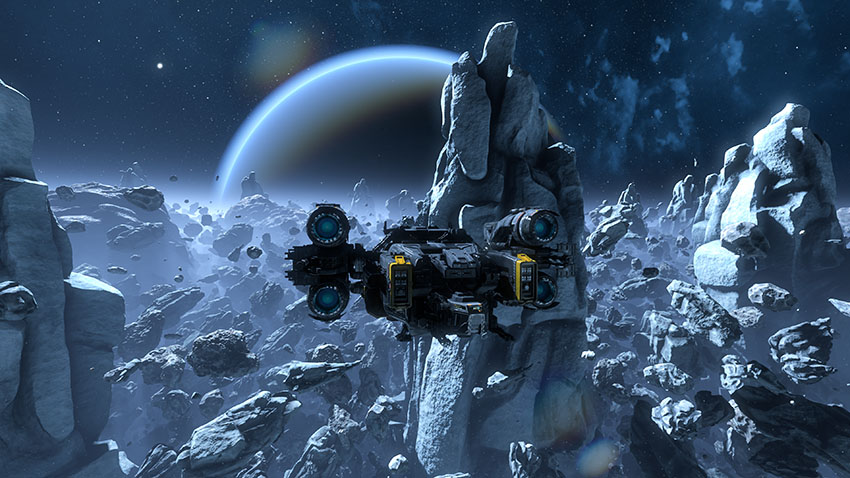
\includegraphics[width=300px]{images/graphics/mesh-shading-asteroids-demo.jpg}
    \caption{The offical \emph{Mesh Shading Pipeline} \emph{Asteroids} demo, featuring the new \emph{Mesh Shading Pipeline} (2018)
    and a high geometric density \cite{Kraemer2018}.}
    \label{fig:mesh-shading-asteroids-demo}
\end{figure}

\noindent
More elaborate algorithms for data computation on the \ac{GPU} led to a further increase in geometrical density.
This is why \emph{NVIDIA} introduced the new \emph{Mesh Shading Pipeline} in 2018 for \emph{NVIDIA Turing} \ac{GPU}s.
This pipeline improves the "old" vertex shader and features a more flexible way of computing and drawing geometry. 
It builds upon some of the innovations presented by Aaltonen et al.  \cite{Aaltonen2015} in 2015. Figure 
\ref{fig:mesh-shading-asteroids-demo} shows a frame of the initial demo provided by \emph{NVIDIA}. The new pipeline is 
discussed in more detail in chapter \ref{sec-mesh-shading} and are a central part of modern games such as \emph{Remedy's}
Alan Wake 2 (\emph{Remedy Entertainment} \cite{AlanWake22023}, 2023) or even \emph{Epic Games'} \emph{Unreal Engine 5} 
\cite{Karis2021}. 


\section{Motivation} \label{sec-motivation}

The latest innovations in computer graphics have been developing in different directions,
one of them being \ac{GPU} Driven Rendering. Minimizing dependencies between \ac{CPU} and \ac{GPU} 
has been an ongoing effort for the last decade. Many of the novel approaches which have been developed 
over the years are visible in the latest technology. But there are still plenty of use cases which are 
not yet living up to their full potential, considering modern hard- and software solutions.\\

\noindent 
One of those use cases is Voxel Rendering. Although there are ongoing efforts to improve voxel 
rendering performance, there are reasons to believe that new innovations can be applied to this 
field of computer graphics. For years, voxel rendering has been using \ac{CPU} and \ac{GPU} 
optimization techniques in order to minimize the data computed by the \ac{GPU}. Many of these 
techniques refer to culling triangles or whole voxels. \ac{CPU} algorithms can make use of the 
regularity of the grid and reduce the amount of triangles sent over to the \ac{GPU}. 
[@TODO: Add sources for gpu acceleration in voxel rendering and write a bit more] \\

\noindent
This poses the question, if advanced culling techniques using modern, \ac{GPU} driven techniques can 
improve voxel rendering. An ideal culling would only draw visible voxels and ignore all other data 
not contributing to the visible and gameplay relevant scene. Therefore, an initial idea involved 
meshlet occlusion culling for large voxel scenes. The use of the new mesh shading pipeline in 
combination with efficient culling could drastically improve frame times. However, as will be 
pointed out in chapter \ref{subsubsec-two-pass-occlusion-culling}, for current occlusion culling 
algorithms to work, objects of different sizes are used to cull smaller instances or even meshlets.
Since voxels are always of the same size, this algorithm cannot be applied as is. The proposed approach 
relies on preprocessing data and applying approximations to the scene layout, so a variation of a 
common meshlet occlusion culling algorithm can be applied. In the next chapter \ref{cpt-related-work}
related work is discussed before an in depth technical foundation is layed out in chapter 
\ref{cpt-technical-background}. 

    \chapter{Related Work} \label{cpt-related-work}

The proposed approach is an aggregation of a lot of ideas and implementations that have been 
around for quite some time. It is of great interest to explore related work, which can provide 
context for use cases and highlight additional techniques that can be adopted additionally. 
This chapter highlights related work addressing \emph{Voxel Rendering}, \emph{Occlusion Culling}, 
and \emph{Mesh Shading}, on which the proposed implementation is based. The most important of 
the highlighted concepts are revisited and discussed in more detail in Chapter 
\ref{cpt-technical-background}. 

[@TODO: Find scientific papers for voxel representations]

\section{Voxel Representation} \label{sec-voxel-representation}

\begin{figure}[h]
    \centering
    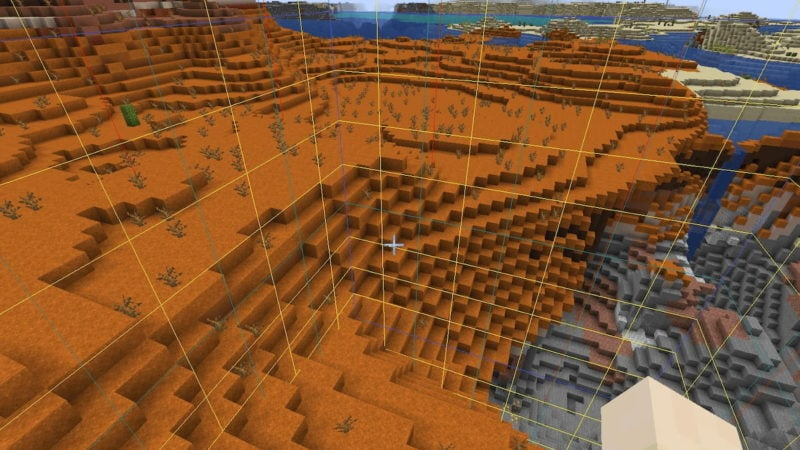
\includegraphics[width=300px]{images/graphics/minecraft-chunks.jpg}
    \caption{A screenshot from \emph{Minecraft}, with a debug visualization of the voxel chunks \cite{Palm2022}.}
    \label{fig:minecraft-chunks}
\end{figure}

\noindent
Voxel Rendering has had huge success in sandbox and highly dynamic games like \emph{Minecraft} (Mojang 
\cite{Mojang2024}, 2011) or \emph{Teardown} (Tuxedo Labs \cite{TuxedoLabs2022}, 2022). Usually these games try 
to preserve some volumetric information for the dynamic environment to be manipulated in real-time. \emph{Minecraft} 
generates a procedural environment based on complex parameters. This way, they can easily generate nearly infinite 
worlds with interesting biomes and landmarks. This huge world is split into chunks of size 16×384×16, to be able to 
stream the world dynamically and allow for quick traversal in any direction, shown in Figure \ref{fig:minecraft-chunks}.
Each chunk maintains its own three-dimensional grid, with the voxel data being highly compressed. Non-existing voxels 
are not being stored, and block states, textures, and other information is stored in per-chunk buffers or as global 
data in a global buffer. This way, using a texture atlas, up to 256 different texture variants can be easily stored 
per voxel by only one byte \cite{Bergensten2012, MinecraftFandom2021}. \\

\noindent
Many other games have made use of voxel rendering, adapting these principles of data compression and data streaming. 
Most optimizations rely on culling voxels, which are not visible, e. g. faces that touch other faces.
Frustum culling and occlusion queries are also part of the optimization process and partially used in \emph{Minecraft} 
as well, though the existence of frustum culling or the specific occlusion culling algorithm added in version 1.5 
cannot be confirmed finally and reliably. Nevertheless, many efforts towards better performance have been made on the 
\ac{CPU} side. Lately, \ac{GPU}-driven approaches have been implemented by various individual developers. 
[@TODO: Find specific optimizations and sources!]  \\

\begin{figure}[h]
    \centering
    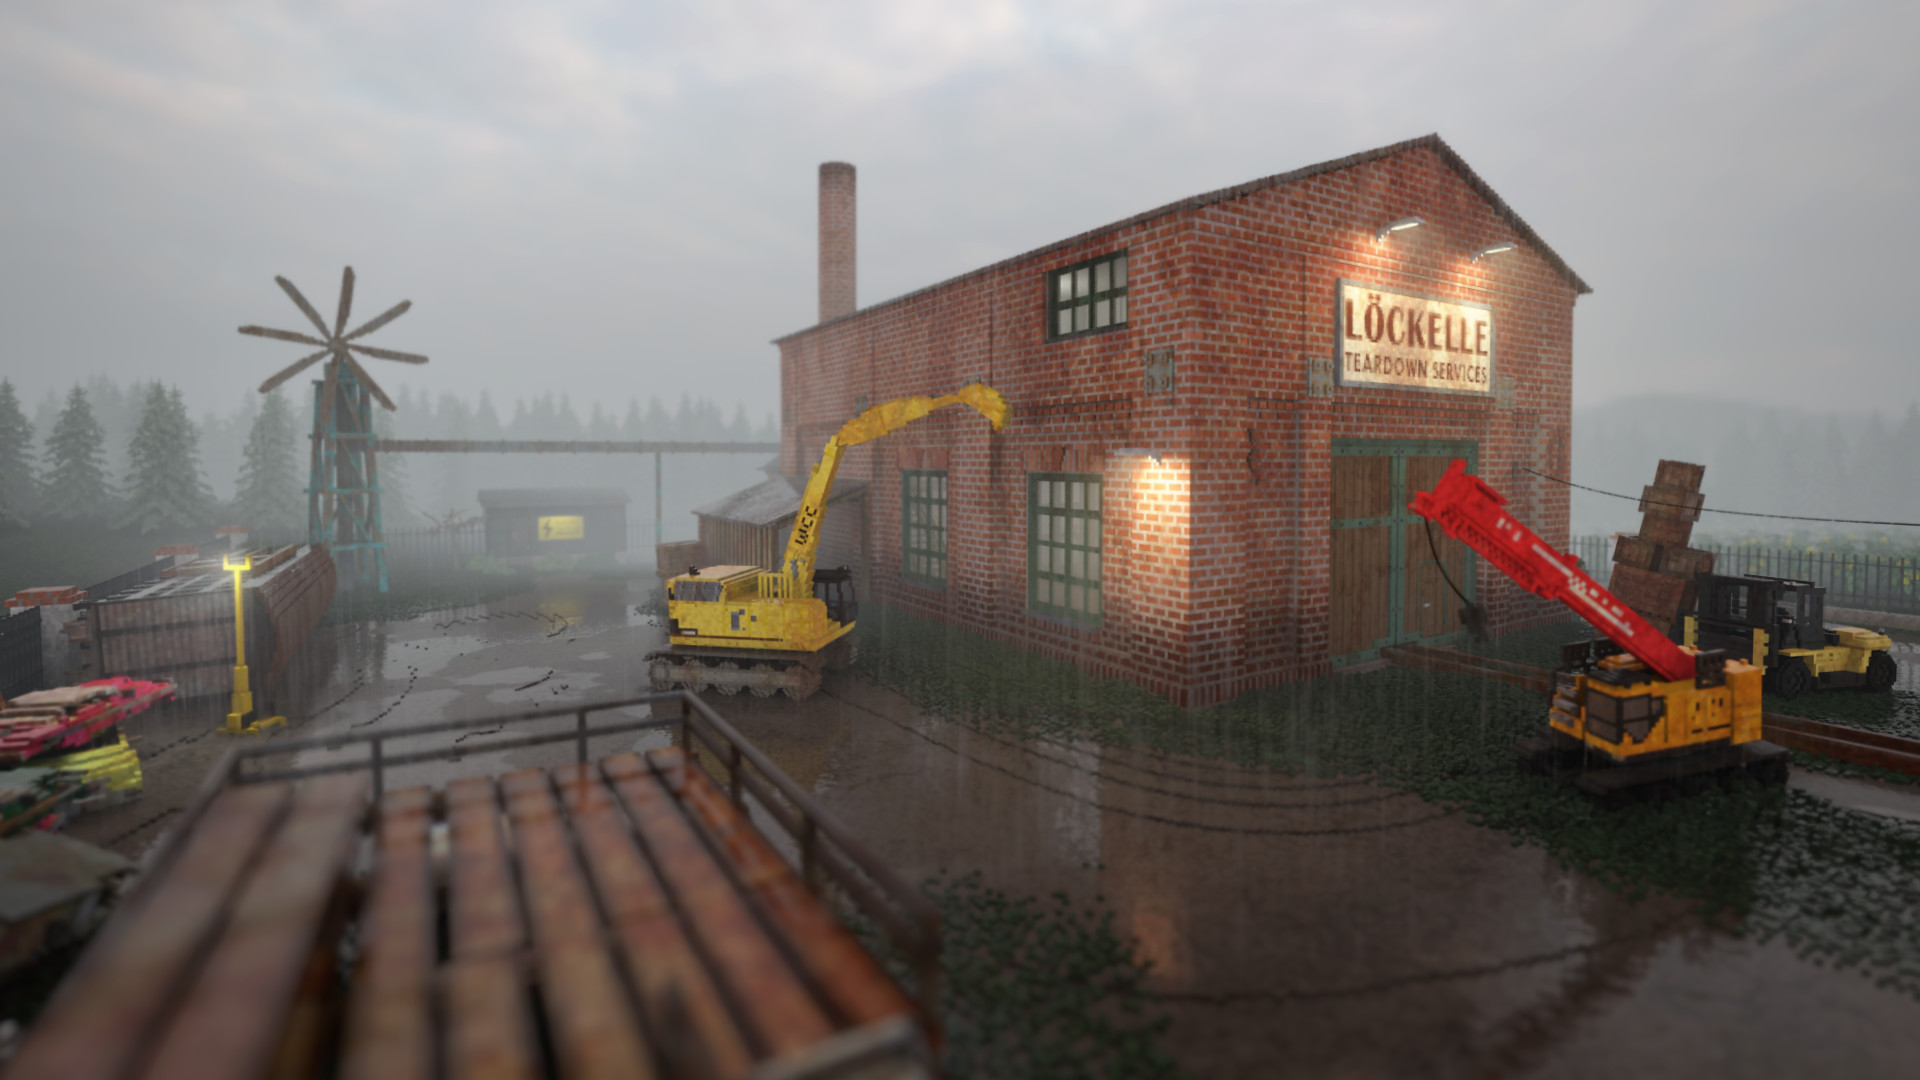
\includegraphics[width=300px]{images/graphics/teardown-ray-tracing.jpg}
    \caption{A screenshot from \emph{Teardown}, showcasing raytraced lighting \cite{TeardownSteam2022}.}
    \label{fig:teardown-raytracing}
\end{figure}

\subsection*{Efficient Sparse Voxel Octrees}

Laine and Karras \cite{Laine2010} analyze and implement a variation of the base Sparse Voxel Octree approach for 
efficiently raytracing voxel models. In their work, contours are used to approximate octree nodes within a \ac{SVO}. If the 
octree node is found to be apprixamted good enough, the subdivision to deeper levels in the octree node is terminated
\cite{Kampe2013,Laine2010}. This way, \ac{SVO}s can be significantly reduced in size, which benefits the memory 
footprint of the application. \\

\noindent
The efficient \ac{SVO}s feature a similar approach to this work in that octree nodes are approximated for faster 
processing times. While Laine et al. use contours for their approximations, this work uses whole octree nodes 
to approximate volumes. \\

\noindent
However, Laine et al. use their implementation for raytraced voxel rendering and the approximations are targeting 
model boundaries only instead of volumes. Therefore, the approximation using contours is not aiming for the same 
optimization than this work's approximation does. While the first one refers to optimizing ray casting, the latter 
refers to optimizing a depth prepass computation.. Nevertheless, both approaches share the aspect of reducing 
octree complexity by approximating parts of the tree hierarchy.


\subsection*{Sparse Voxel Directed Acyclic Graphs}

Kämpe et al. \cite{Kampe2013} propose the use of their \emph{High-Resolution Sparse Voxel \ac{DAG}s}. This approach 
is tailored to high voxel resolutions and data that might not fit into memory all at once. Their data structure can 
be easily split up into several sub-trees, which in turn can be loaded individually. This approach seems promising 
for large scenes and use cases, which require the streaming of data. They propose to structure the data in a way that 
enables equal nodes of an octree hierarchy to be reduced to only one instance, eliminating redundant parts of the 
hierarchy and reducing the amount of used memory immensely. \\

\noindent
This approach relates to this implementation in how large voxelized scenes can be efficiently loaded and stored in 
memory. Although this work doesn't explicitly rely on Sparse Voxel \ac{DAG}s, Sparse Voxel octrees are used in the 
provided implementation. Additionally, the proposed implementation can be optimized in the future to be working 
with Sparse Voxel \ac{DAG}s, enabling the handling of meshes with even higher resolution. \\

\noindent
Sparse Voxel \ac{DAG}s are not commonly used in rasterized rendering pipelines and store voxlumetric data in a binary 
format instead of storing positional data. This introduces additional complexity to the pipeline, which might result in 
better runtime performance but is also less intuitive when dealing with nodes and individual voxels. Sparse Voxel 
\ac{DAG}s mainly aim to provide a smaller memory footprint for raytraced applications while maintaining high resolution 
voxel meshes. \\

\noindent
Compared to this work's approach, Sparse Voxels \ac{DAG}s are able to resolve voxel data more efficiently and is 
better suited for higher resolution meshes that might exceed memory limits in a raw data format. However, their 
primary usage is ray-traced rendering which is not what this work is concerned with. While Sparse Voxel \ac{DAG}s 
could generally be applied to rasterized rendering, this work uses a custom Sparse Voxel Octree, optimized for 
traversal and easy coordinate extraction. 


\section{Occlusion Culling}


\subsection*{Hierarchical Z-Buffering}

Greene et al. \cite{Greene93,Greene95} proposed the first \ac{HZB} algorithm with the capability to use screen space 
data to cull meshes in large and densely populated scenes. The idea originated in the context of a forward rendered 
pipeline, making use of the \ac{CPU} for culling instances. They propose to use a spatial container like an octree to 
enable drawing the scene in a rough front-to-back order. Each mesh is individually drawn to a depth buffer resource, 
starting with an empty one in the beginning and populating it as more meshes are drawn. The buffer resource also 
maintains a mip chain that is updated when the full resolution depth buffer is updated. Each time a mesh is rendered 
to the depth buffer, it is checked against the depth hierarchy, starting with the coarsest mip level. This way, near 
and big objects are likely to occlude small, far objects, resulting in an efficient way to reject invisible meshes.\\

\noindent
Although this technique was intended for use on the \ac{CPU}, it can be easily adapted to work on \ac{GPU} resources 
without the need of a write-back to expose the data to \ac{CPU} memory. The approach by Greene et al. is the basis for 
modern \ac{GPU} based algorithms and a major influence for the work at hand. It uses the same principle of hierarchical 
visibility testing and maintaining a depth buffer. \\

\noindent
However, more modern approaches are used to adapt this algorithm for \ac{GPU} friendly design, like computing the depth 
in a pre-pass, using only best occluders instead of all possible meshes, and disabling color writes completely. This also 
limits the amount of recomputations of the mip-chain since all occluders are only drawn to the depth buffer once per 
frame instead of scaling with the number of visible meshes.

\subsection*{Umbra}

In the past, occlusion culling in games has been heavily influenced by \emph{Umbra} \cite{Umbra2024}, a company 
specializing in 3D occlusion culling solutions. \emph{Umbra} has been used by a lot of games such as 
\emph{Call of Duty: Ghosts} (2013), \emph{Killzone: Shadow Fall} (2013), \emph{Alan Wake} (2012), and many more 
\cite{UmbraWiki,CallOfDutyGhostsCredits,KillzoneUmbra,AlanWakeUmbra}. \\

\noindent
\emph{Umbra} voxelizes the game world and proceeds to process the data further, merging voxels into cells. 
A runtime hierarchy of the meshes inside the voxelgrid is created and subsequently, using the camera position, 
the cells can be queried for occlusion. As long as there are large occluders, this process can reduce the number 
of instances and therefore the number of triangles to draw. \emph{Umbra} also keeps a simplified depth buffer in 
memory in order to quickly determine visibility \cite{Medium2018}. \\

\noindent 
The approach is similar to the approach provided  in this work, in that both use a depth buffer and a scene hierarchy 
for computing visibility early in the pipeline. Both approaches rely on screen-space bounding comparisons, although 
\emph{Umbra} uses a \emph{Portals and Cell} structure to manage visibility testing for a given camera position 
\cite{Medium2018}. Furthermore, \emph{Umbra} is usually applied in triangle mesh scene representations instead 
of volumetric, voxel-based scene representations. \emph{Umbra} uses runtime data structures for efficient visibility 
optimizations based on static scene meshes, while this work uses octree queries to dynamically determine possible 
occluders during runtime - or as a one-time pre-computation for voxel models that are known to be static. \\


\subsection*{Two-Pass Occlusion Culling}

\noindent [@TODO: Remove AC Unity and only focus on Aaltonen]
\emph{Assassin's Creed Unity} (2014) uses a \ac{GPU} based two-pass occlusion culling technique as presented by 
Aaltonen et al. \cite{Aaltonen2015}. This technique involves both \ac{HZB} and depth reprojection. Both make for 
a good occlusion culling technique in games with large occluders or interiors. First, artist picked 
\emph{best occluders} are drawn to the depth buffer in a depth pre-pass. Then, projected bounding boxes can be 
used to test the visibility of smaller objects in the scene. A hierarchical z-buffer is used to accelerate this 
testing, as proposed by Greene et al. \cite{Greene93,Greene95}. Finally, the depth buffer of the last frame can be 
reprojected to further minimize computations. This technique allows developers to push for huge draw distances and 
densely crowded environments.\\

\noindent
Similar to this work, the game uses advanced technology in its implementation, clustering geometry, and allowing 
for a \ac{GPU} centric approach to occlusion culling. However, the game doesn't use a volumetric representation 
but the standard boundary representation for its world. Furthermore, the best occluders are provided in different 
ways. Aaltonen et al. \cite{Aaltonen2015} propose the use of a hand-picked set of large, static meshes, while this 
work relies on a simple approximation of the voxel layout. This way, the latter implementation can dynamically 
provide best occluders during runtime, adapting the occlusion capabilities with the addition or removal of voxels 
in the scene.


\subsection*{Masked Software Occlusion Culling}

Hasselgren et al. \cite{Hasselgren2016} present a novel way of implementing occlusion culling relying on hardware 
occlusion queries while optimizing the queries using \ac{CPU} \ac{SIMD} acceleration. The basic algorithm is very 
similar to common \ac{CPU} or \ac{GPU} computed \ac{HZB}, with two major alterations to the implementation. First, 
they make use of Intel's \ac{AVX} to compute depth values for tiles of 256 texels in parallel. The second difference 
is the way they store depth and coverage data. In contrast to a "normal" \ac{HiZ} mip-chain, Hasselgren et al. 
decouple depth and coverage data by storing a coverage mask for \begin{math}32 \times 8\end{math} pixel tiles, 
which can be efficiently computed by using the \ac{AVX} of Intel \ac{CPU}s. In their results, they show that their 
implementation is up to 3 times faster than previous occlusion culling algorithms while also providing a lower 
memory footprint. \\

\noindent
The work of Hasselgren et al. relates to this work's implementation in the general concept of occlusion culling, making 
use of projected bounding boxes, and a comparison of minimal z values. Their work shows that such an algorithm can be 
optimized for \ac{CPU} execution using \ac{SIMD} and effective use of data structures. \\

\noindent 
In contrast to this work, Hasselgren et al. use their algorithm for non-volumetric triangle meshes. This means that 
they make heavy use of raster occlusion queries, making rendering CPU-bound. While still efficient and possibly faster 
than \ac{HZB}, Masked Software Occlusion Culling lacks the \ac{GPU} driven basis for this work's implementation. This 
work's approach does not work with geometry on the \ac{CPU} side at all but leaves all of the triangle computations up 
to the last possible stage of the pipeline, making the application of \ac{CPU} accelerated occlusion queries impractical.


\subsection*{Per-Meshlet Two-Pass Occlusion Culling}

Similar to \emph{Assassin's Creed Unity}, the game \emph{Alan Wake 2} (2023) and engine \emph{Unreal Engine 5} also 
implement \ac{HZB} and depth reprojection. Both implementations are directly based on the approach of Aaltonen et 
al. \cite{Aaltonen2015}, but this time, making use of the new \emph{Mesh Shading} pipeline. The difference being the 
now provided hardware integration of clustering geometry \cite{Remedy2023,Karis2021}.  \\

\noindent
Karis et al. and Remedy Entertainment find that using \ac{HZB} can provide great runtime performance for open, 
highly dense scenes. Both combine the \ac{HZB} with depth reprojection to further optimize the computation of the 
depth buffer. Using the Mesh Shading pipeline, this concept can be applied to meshlets, enabling per-meshlet culling. 
That means that small parts of the geometry can be culled, even if other parts of the same mesh are still visible. 
This optimizes the culling further so scenes can be more densely populated with meshes.\\

\noindent
The findings of Karis et al. and Remedy Entertainment are adapted for this work's implementation, which also relies on 
the use of the Mesh Shading pipeline. While the implementations of Karis et al. and Remedy Entertainment are based on 
a boundary representation and do not require the use of a spatial container for the culling algorithm, this 
implementation aims for a different use case. Contrary to boundary representations, the spatial properties of voxels 
can be used to approximate volumetric coverage by less complex geometry, making it more efficient to select and draw 
best occluders. Also, this work uses the best occluders not only to occlude meshlets, which are behind the best occluders, 
but it can additionally be used to occlude parts of the best occluders itself. This poses a new way of applying occluders 
in the context of rendering volumetric scenes.


% SV DAGs
% AC Unity
% Alan Wake 2
% Greene
% Raster OC using depth queries -> not viable for so many objects
    \chapter{Technical Background} \label{cpt-technical-background}

\section{Voxel Scene Layout}

The voxel rendering in our evaluation relies on a volumetric representation of the scene.
It is particularly important that the voxel model not only includes the surface but also 
the space within the model. This constraint is often used in interactable use cases, where 
the model is split, cut or manipulated in any given way. [@TODO: Reference] \emph{Minecraft} 
lets the player take full control over the sandbox environment and allows adding or subtracting 
voxels as they wish. Essentially, the voxel data of every possible voxel within the playable 
space needs to be somehow present or encoded in memory, even though just a fraction of the 
voxels are actually drawn to the screen.\\

\subsection{Three Dimensional Grid} \label{subsec-three-dimensional-grid}

[@TODO: Additional option of drawing bitwise]
A basic approach for a scene representation is a three dimensional voxel grid. This 
approach relies on a fixed size grid where each grid cell represents one voxel.
To draw the voxels, a separate buffer can hold additional voxel information, which 
can be accessed by a given grid cell index. The voxel data can store information about 
whether a voxel is present in that particular grid cell or not, which color the voxel 
should have, the normals for lighting calculation and any other data necessary.
This approach is relatively lightweight but inefficent for large grid sizes and low 
grid occupations. All grid cells need to be traversed to draw any given scene which 
might include a lot of empty grid cells. Additionally, storing the voxel data seperately
introduces a pointer indirection on each step of the traversal, potentially leading to more 
cache misses.

\subsection{Octree Data Structure} \label{subsec-octree-data-structure}

[@TODO: source] proposes the use of a spatial container to optimize traversal. The use of an octree 
incorporates the relevant scene space and subdivides it into smaller child nodes. When inserting data 
into the octree, the position is evaluated and the data is being stored as a \emph{payload} in 
a node which includes the given position. If a node holds more payload instances than a specified threshold 
allows, it is split into eight child nodes and the payload originally present in the node is 
distributed onto the child nodes. This process is repeated until all data is finally inserted 
into the octree. The resulting octree maintains all the relevant payload data, having a deeper tree 
hierarchy where more data is present and a shallow hierarchy where almost no or no data is present.

\begin{figure}[h]
    \centering
    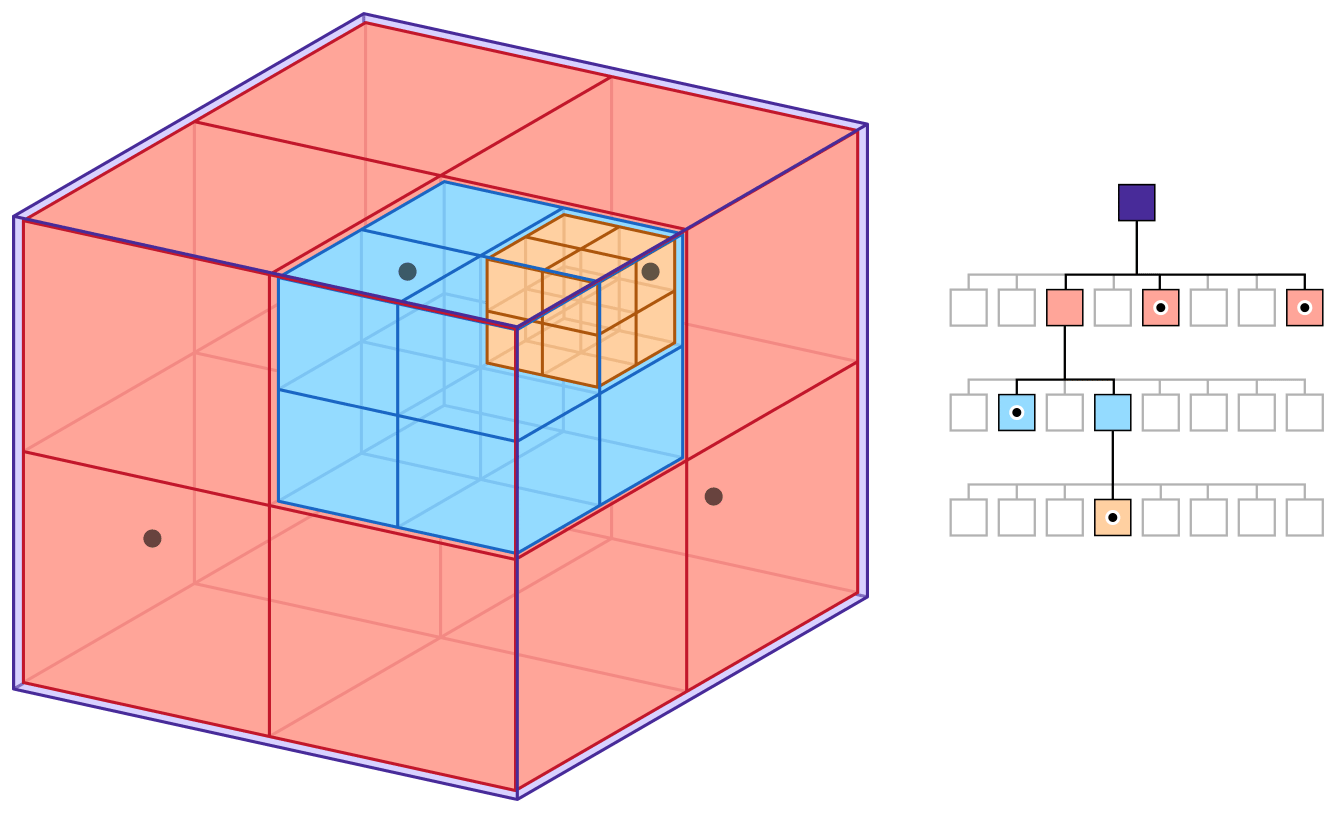
\includegraphics[width=300px]{images/graphics/octree.png}
    \caption{An octree data structure. It stores data alongside its spatial characteristics, relative to 
    other data entries \cite{Six2021}.}
    \label{fig:octree}
\end{figure}

[@TODO: Mention other spatial containers -> Binary Space Partitioning Trees]

Octrees like this can vary in their specific implementation, especially in how they maintain the 
payload. Some might store it right next to the octree node description, others might want to separate 
octree and payload data. Octree nodes could also be appended to a dedicated buffer and therefore be stored 
separately from the tree hierarchy description. Such an approach would maintain cache coherency during an 
unordered traversal of all octree nodes. [@TODO: find appropriate sources]

When using hierarchical data structures, dedicated vertex positions can be omitted and instead 
the voxel position in space can be implicitly calculated from the hierarchy and the root node's bounds. 
This allows for improvement of memory occupation, which is vital for loading and storing high 
resolution voxel scenes. A voxel's state can be encoded into either visible (1) or empty (0).
A bitwise representation of voxels can significantly decrease the memory footprint, that the next 
approach expand on.

\subsection{High Resolution Sparse Voxel Directed Acyclic Graphs} \label{subsec-highres-svo-dags}

Assarsson et al. \cite{Assarsson2013} use data redundancy to further generalize and optimize high resolution 
\ac{SVO}s. In their implementation, the octree data structure relies on bitmasks, to encode the existence of child 
nodes. This way, empty nodes are ignored and the information can be easily stored within one byte. This child node 
mask uniquely identifies the layout of the nodes below and can also be used to store the voxel occupation of the 
leaf nodes. Next, they make use of the fact that an octree node's position is uniquely identifed by the path along 
the nodes from root to leaf node. Since voxels can be encoded as either being present or not, and non-present 
voxels can be ignored, the data can be significantly reduced in size. Furthermore, equal child node masks 
can simply be shared between different parent nodes instead of being duplicated. Assarsson et al. \cite{Assarsson2013} 
suggest a bottom-up approach to remove redundant nodes and replace whole sub-trees of the octree by pointing to one 
instance of the same pattern within the tree, which is shown in figure \ref{fig:sparse-voxel-dag-creation}. 
This optimization can be recursively done to each layer in the tree hierarchy, resulting in an optimized version 
of the data structure. The resulting structure is a more general hierarchical data structure, namely a \ac{DAG}.

\begin{figure}[h]
    \centering
    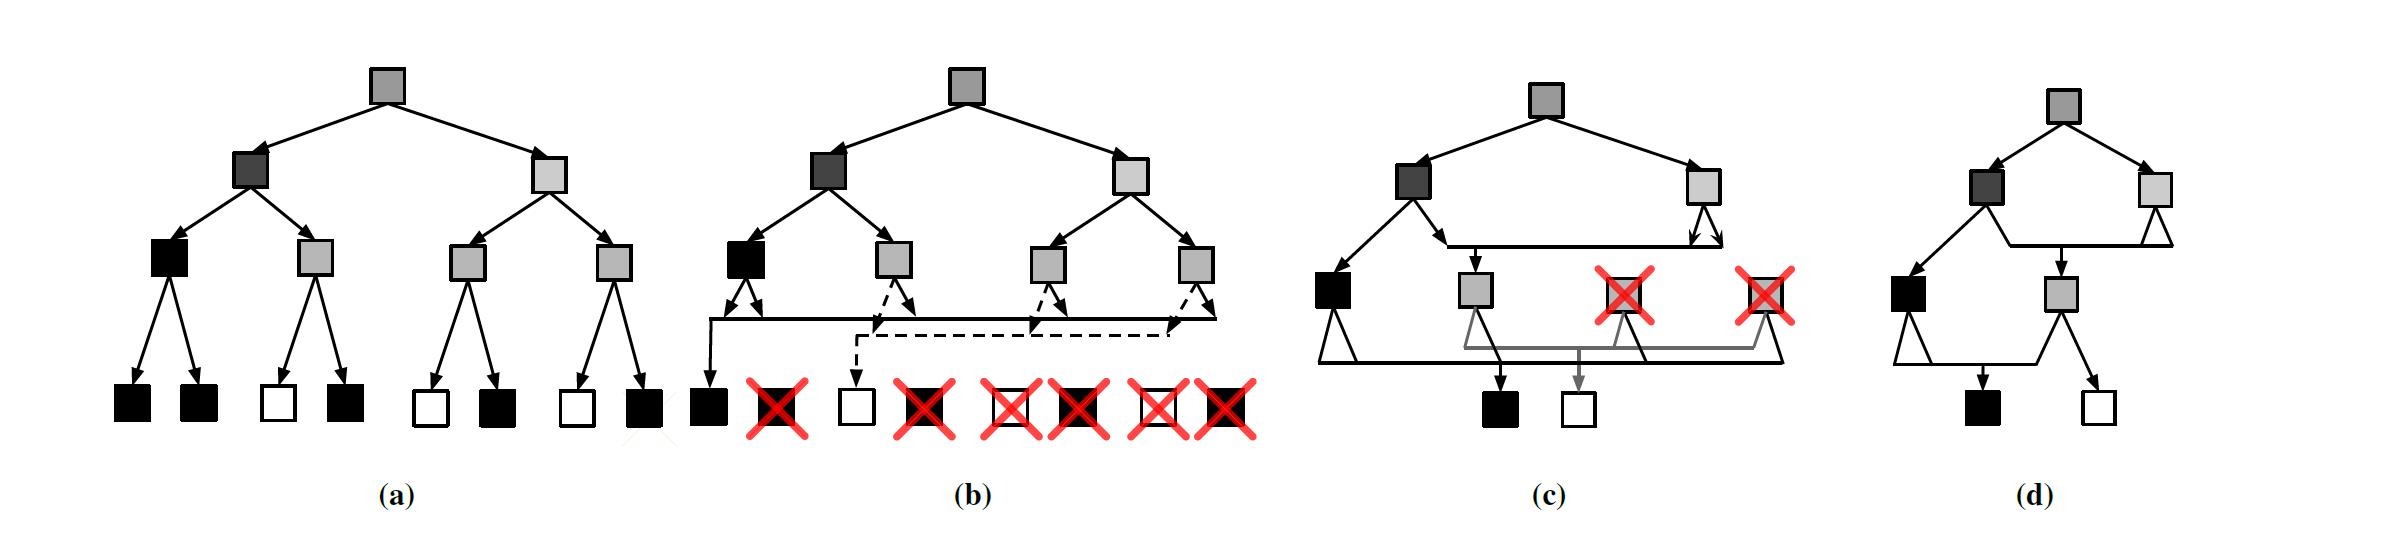
\includegraphics[width=\linewidth]{images/graphics/highres-sv-dag.png}
    \caption{Reducing a \ac{SVO} using the approach of \cite{Assarsson2013}.}
    \label{fig:sparse-voxel-dag-creation}
\end{figure}

\noindent
This approach seems to be the best solution for reading, storing and optimizing octree data, although we use 
a more basic approach in our implementation. Nevertheless, this concept of optimizing voxel data is compatible 
with our use case and is highly recommended by us.

\section{Culling Techniques} \label{sec-culling-techniques}

\emph{Culling} refers to the technique to discard parts of a scene "that are not considered to contribute to the final 
image" \cite{AkenineMoeller2018}. This allows for highly populated scenes to be rendered, since most parts of a scene 
will probably not be visible by the camera at the same time. Ignoring culled objects or triangles is therefore a common 
process in real-time rendering. "The fastest triangle to render is the one never sent to the \ac{GPU}" 
\cite{AkenineMoeller2018}. In this section, the most common culling techniques are presented and the ones considered by 
our approach are specifically highlighted and analyzed. 


\subsection{Backface Culling} \label{subsec-backface-culling}

[@TODO: Rework sentence or find source]
Backface culling is probably the most commonly used culling algorithm. It is concerned with discarding triangles that 
are facing away from the camera. These triangles will not be seen by the camera anyway and thus can be safely ignored 
in the rendering process. To compute the facing direction of a triangle, which when normalized is equivalent to the 
triangle's \emph{Surface Normal}, the vertex \emph{winding order} of the given rendering backend is considered.\\

\begin{figure}[h]
    \centering
    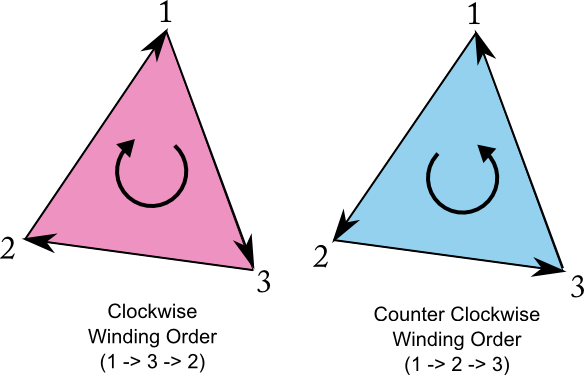
\includegraphics[width=200px]{images/graphics/winding-order-triangle.png}
    \caption{Two possible winding orders of triangles \cite{Michel2016}.}
    \label{fig:triangle-winding-order}
\end{figure}

\noindent
When describing a triangle mathematically, the vertex positions are considered, which perfectly define the edges of 
said triangle. The surface can then be interpreted as facing towards the viewer or away from them. 
When trying to compute the triangle, its vertex positions can be recorded in an arbitrary order, but to encode which 
direction the surface is facing, the vertex position order is specified up front. Microsoft's rendering \ac{API}s D3D11 
and D3D12 for example encode a counterclockwise winding order to be interpreted as facing towards the viewer 
\cite{D3DTopology2020}. With this standard in place, all triangles can uniquely define their orientation relative to 
the camera. When enabling backface culling within the rendering backend, triangles which are not facing the camera 
are automatically omitted immediately after screenmapping \cite{AkenineMoeller2018}. Depending on the type of geometry, 
backface culling can remove up to half of the triangles about to be rendered, proving very valuable to highly populated 
scenes and high geometric density.\\

\noindent 
[@TODO: Add image]
Backface culling algorithms can also be applied to clusters of triangles. As Shirmun et al. \cite{Shirmun1993} propose, 
multiple triangles can be culled at once considering a common normal cone. "Shirmun and Abi-Ezzi \cite{Shirmun1993} 
prove that if the viewer is located in [a] frontfacing cone" constructed by the normals of all the triangles within the 
cluster, "then all faces in the cone are frontfacing, and similarly for the backfacing cone" \cite{AkenineMoeller2018}. 
As will be mentioned in chapter \ref{subsubsec-meshlet-backface-culling}, this approach can be used for more 
parallelized backface culling using an updated rendering pipeline in current graphics \ac{API}s.

\subsection{View Frustum Culling} \label{subsec-view-frustum-culling}

[@TODO: Add pictures]

\emph{View Frustum Culling} is a technique that aims to remove instances, i.e. meshes, which are outside of the camera 
view frustum. This leads to the skipping of all instances that are completely invisible due to their location relative to 
the camera. Said instances can thus be safely ignored and discarded early in order to keep the memory occupation low. 
To cull potantial instances, bounding boxes are calculated and checked against the camera view frustum, which in turn 
is specified by the \emph{near plane} and \emph{far plane}, as well as the \emph{fov}, encoded in a \emph{dot-normal}
representation. For instance, testing if a bounding sphere is partially or completely inside the view frustum can be 
computed with the following algorithm: \\

\begin{algorithmic}[1]
    \State $radius \gets \text{GetBoundingSphereRadius()}$ 
    \State $center \gets \text{GetBoundingSphereCenter()}$ 
    \State $planeIndex \gets 0$
    \While{$planeIndex < 6$}
        \State $planeIndex \gets planeIndex + 1$
        \State $frustum \gets \text{frustumPlanes}[planeIndex]$ 
        \State $distance \gets \text{dot}(frustum, center)$
        \If{$distance < -radius$}
            \State \Return \textbf{FALSE}
        \EndIf
    \EndWhile
    \State \Return \textbf{TRUE}
\end{algorithmic}

\vspace{0.5cm}
\noindent
In combination with acceleration structures like an octree, view frustum culling can be computed for the bounding 
volumes of the given structure, which can further optimize the culling operations due to spatial grouping of multiple 
instances. This technique is also applied in our approach, using spheres as approximations for the cubical octree 
bounding volumes.

\subsection{Occlusion Culling} \label{subsec-point-based-occlusion-culling}

When considering highly populated scenes, there might be cases of meshes occluding other meshes. This produces overdraw 
when rasterizing the final projection, which means that multiple color values will be calculated for the same pixel 
before the final color is determined. In general, overdraw should be avoided where possible. Having a lot overdraw 
within the rendering process means that visibility determination of instances is deferred to the last possible point in 
the rendering pipeline. Often, it is better to pre-determine visibility and sample only visible instances. To achieve 
this, algorithms can be used to select and omit occluded instances. \\

\begin{figure}[h]
    \centering
    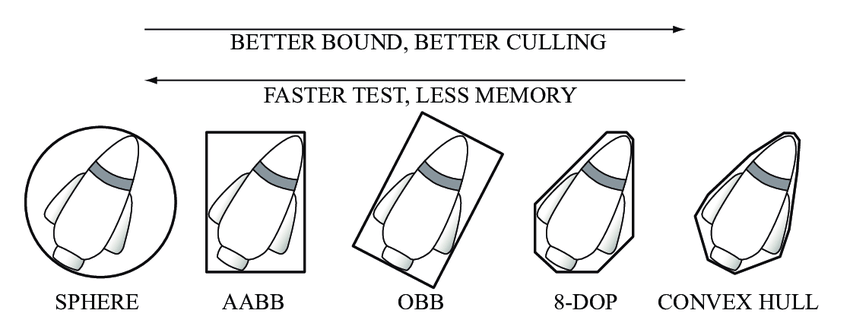
\includegraphics[width=300px]{images/graphics/bounding-volume-quality.png}
    \caption{Different bounding volumes provide different advantages and disadvantages \cite{Six2021}.}
    \label{fig:bounding-volumes}
\end{figure}

\noindent
Different occlusion culling algorithms can be applied depending on scene layout, object characteristics and other factors.
As it is the case with culling algorithms in general, occlusion culling algorithms usually rely on bounding volumes to 
approximate object positions and scale in space. Figure \ref{fig:bounding-volumes} shows how different bounding volumes 
can be used to support faster computation or more accurate volume approximation. Algorithms have been proposed which 
operate in \emph{image space}, \emph{object space} or \emph{ray space}, with image space occlusion culling being most 
widely adopted in real-time rendering \cite{AkenineMoeller2018}. These algorithms operate on a projected 2D image to 
consider visibility of different instances.  

\subsection{Hierarchical Z-Buffering} \label{subsec-hierarchical-z-buffering}

\emph{\ac{HiZ} Buffering} is a technique first introduced for \ac{CPU} computation by Ned Greene et al. 
\cite{Greene93,Greene95}. Since then, it "has had significant influence on occlusion culling research" 
\cite{AkenineMoeller2018}. It is a fundamental basis on which our approach relies on, which will be discussed 
in more detail.\\


[@TODO: explain texel (?), mip levels]
\begin{figure}[h]
    \centering
    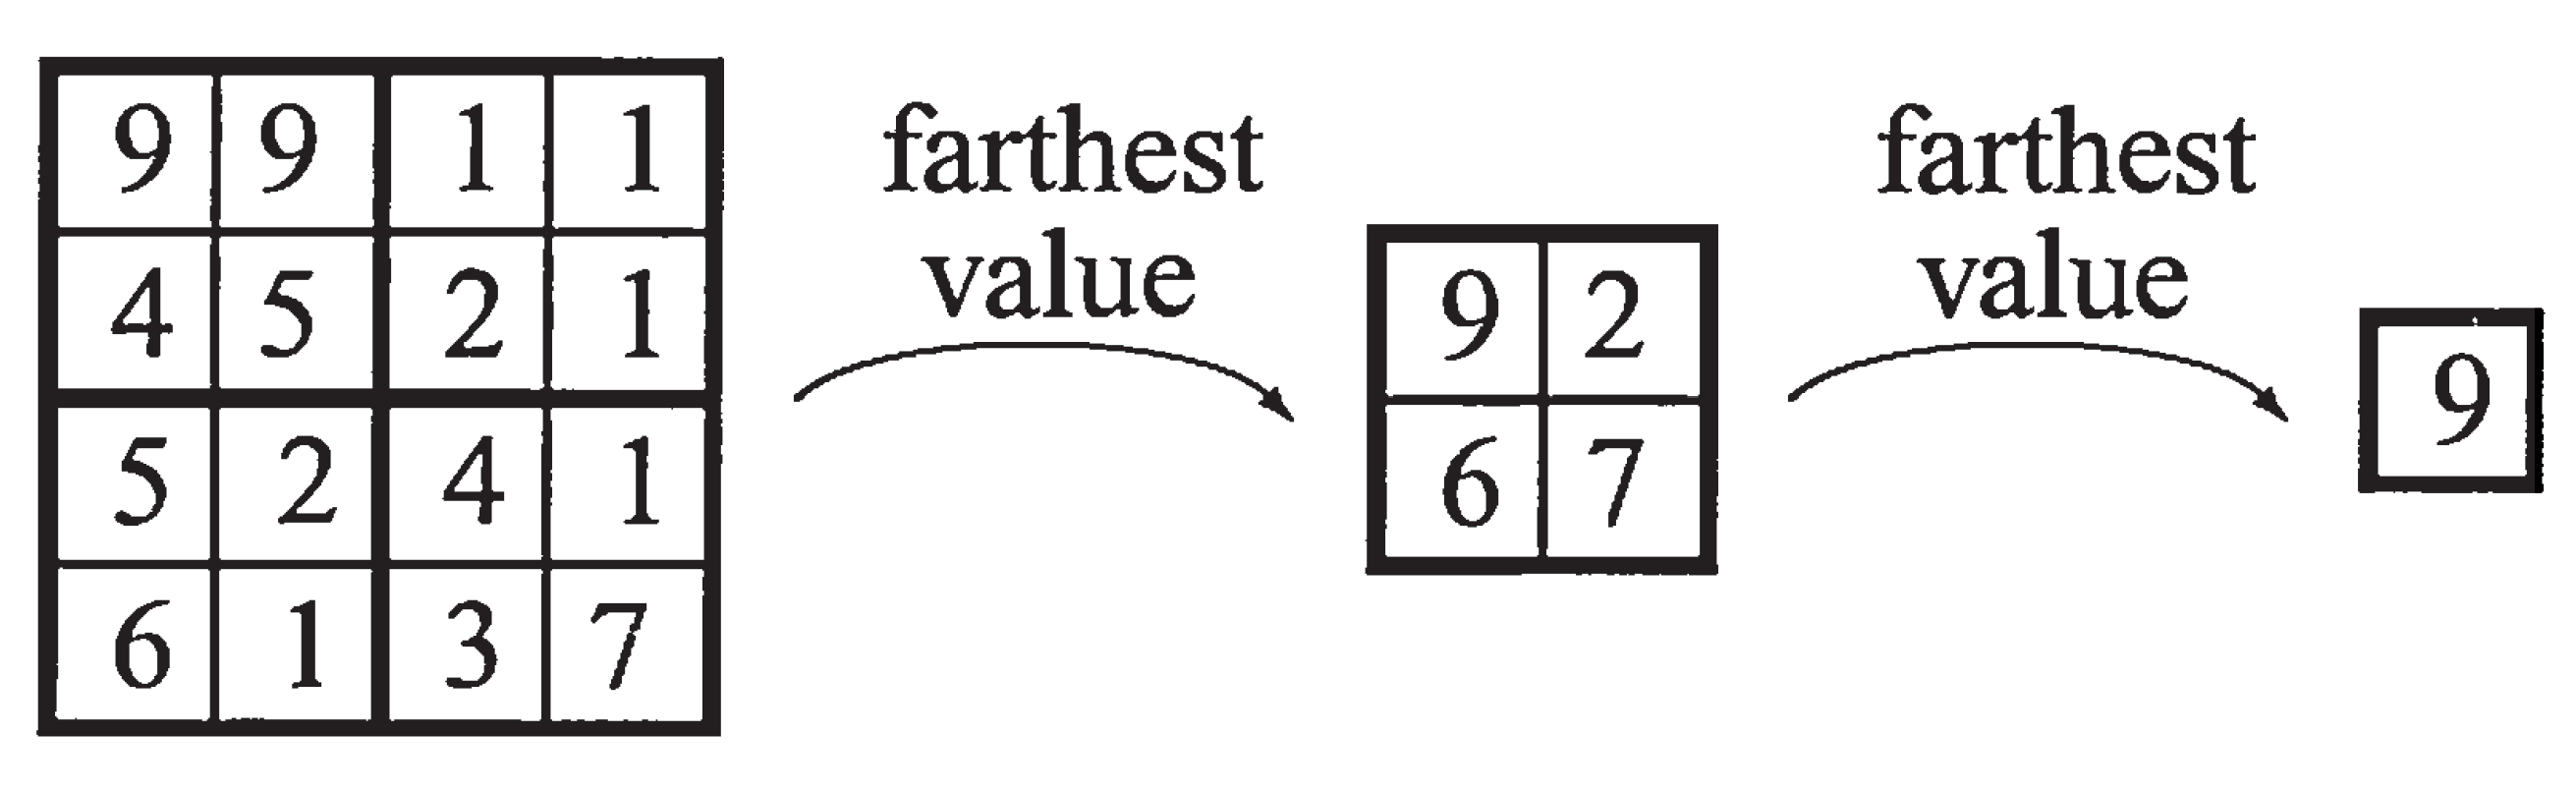
\includegraphics[width=200px]{images/graphics/hiz-buf-values.png}
    \caption{The calculation of a \ac{HiZ} buffer computes the farthest value of each texel window, 
    resulting in a new texel value for adjacent mip levels \cite{AkenineMoeller2018}.}
    \label{fig:hiz-value-computation}
\end{figure}

\noindent
\ac{HZB} is computed in image space and relies on two main components. An octree scene representation and a 
\emph{z-buffer} pyramid. [@TODO: Check if z-buffer or mip-map needs to explained] 
The octree contains all instances present in the scene. The \emph{z-pyramid} is a set of z-buffer mip-maps, with every 
map reducing in size relative to the previous mip-map. The reduction is computed by aggregating values from 4 texels 
within the previous mip-map and writing the output value into one texel of the new mip-map level. This way, both axes 
(u and v) are scaled to be half the length of the previous level. The resulting z-pyramid then has the full resolution 
z-buffer as the finest granularity in the z-pyramid and a very low resolution and small texture on the other end. 
An exemplary z-pyramid is shown in figure \ref{fig:hiz-mip-chain}.\\

\noindent
The computation of new values is another crucial step. "[...] [E]ach z-value is the farthest z in the corresponding 
2 \begin{math}\times\end{math} 2 window of the adjacent finer level" \cite{AkenineMoeller2018}. This process is shown 
in figure \ref{fig:hiz-value-computation}, showing how the farthest value of each texel window is inserted into adjacent 
levels.\\

\begin{figure}[h]
    \centering
    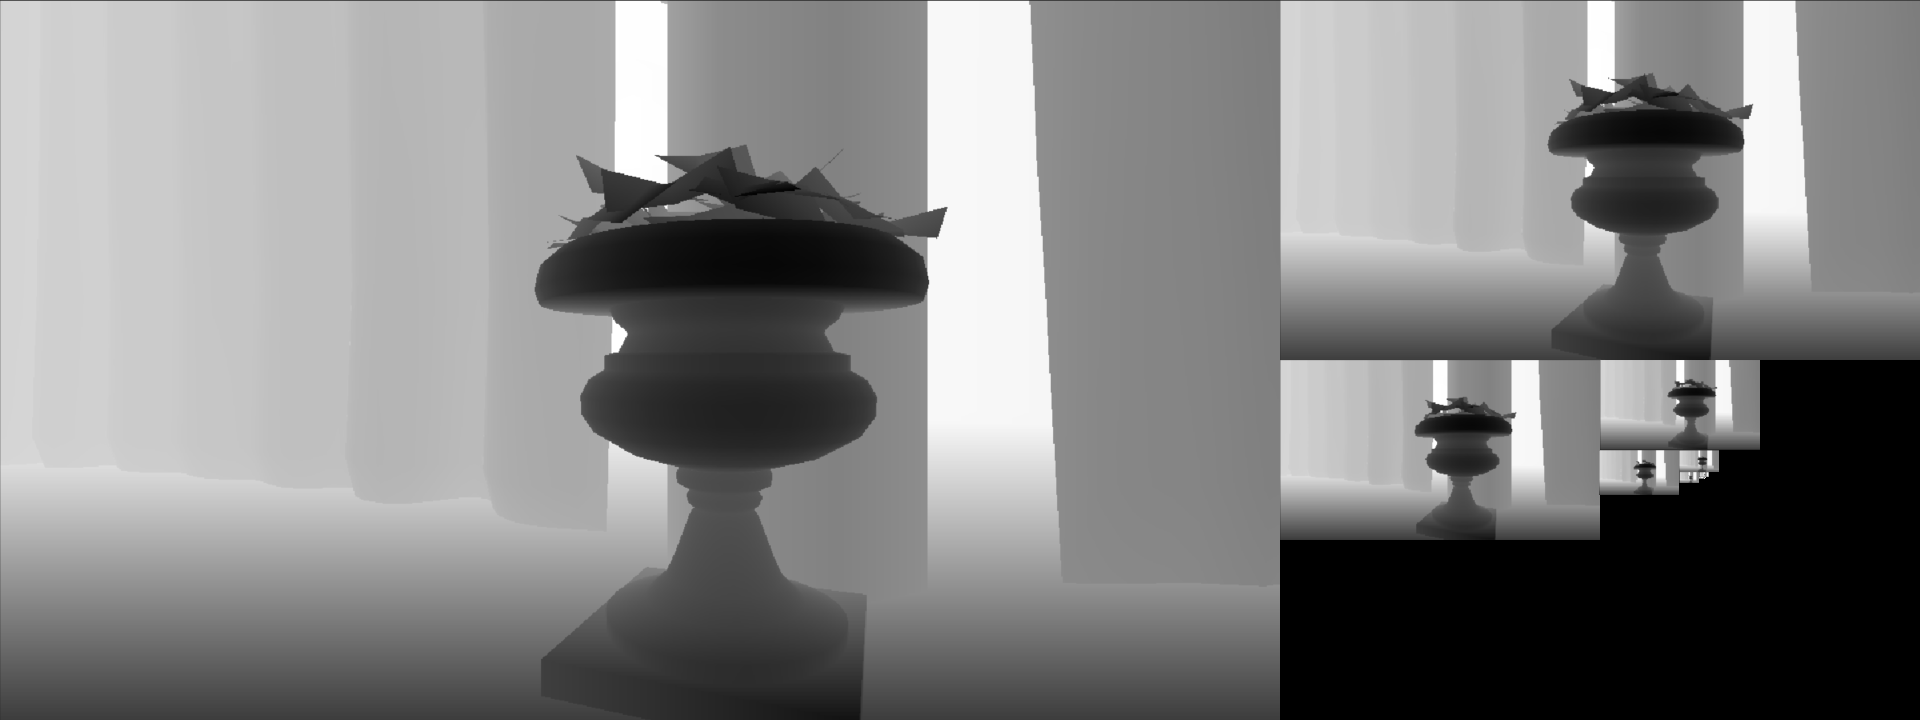
\includegraphics[width=\linewidth]{images/graphics/hiz-mip-chain.png}
    \caption{A mip chain of a scene's z-buffer. Every buffer in this chain is a quarter of the resolution of its 
    predecessor buffer \cite{Schachtschabel2017}.}
    \label{fig:hiz-mip-chain}
\end{figure}

\noindent
A visibility test against this z-pyramid is computed as follows: The octree is traversed in a front to back order 
and each octree node is transformed into image-space, essentially projecting the bounding volume of the node onto 
the view plane. Now, the projected bounding volume overlaps a specific region of the view plane, which is then 
tested against the coarsted z-pyramid cell, containing this volume projection. The nearest z value of the bounding 
volume is compared to the z-pyramid's farthest value entries. If the bounding volume's z happens to be farther than the 
\ac{HiZ} value, it is consequently occluded. If the comparison yields the opposite result, the test "is continued 
recursively down the z-pyramid until the [bounding volume] is found to be occluded, or until the bottom level of the 
z-pyramid is reached, at which point the box is known to be visible" \cite{AkenineMoeller2018}. Visibile octree nodes 
are then drawn to the depth buffer, meaning all the geometry contained within the node is drawn to the depth buffer 
for being tested against during the computation of the following octree nodes. As Akenine-Möller et al. 
\cite{AkenineMoeller2018} point out, this algorithm is not used in its original form. Modern variations of this 
algorithm evolved from the work of Greene et al. \cite{Greene93} and are widely adopted in modern real-time computer 
graphics. As will be shown in chapter \ref{subsec-two-pass-occlusion-culling}, the concept of an octree representation 
used for hierarchical culling and a z-pyramid used as an occlusion representation (\cite{AkenineMoeller2018}) can be 
elegantly leveraged on the \ac{GPU} side for efficient occlusion culling.


\subsection{Two-Pass Occlusion Culling} \label{subsec-two-pass-occlusion-culling}

\begin{figure}[h]
    \centering
    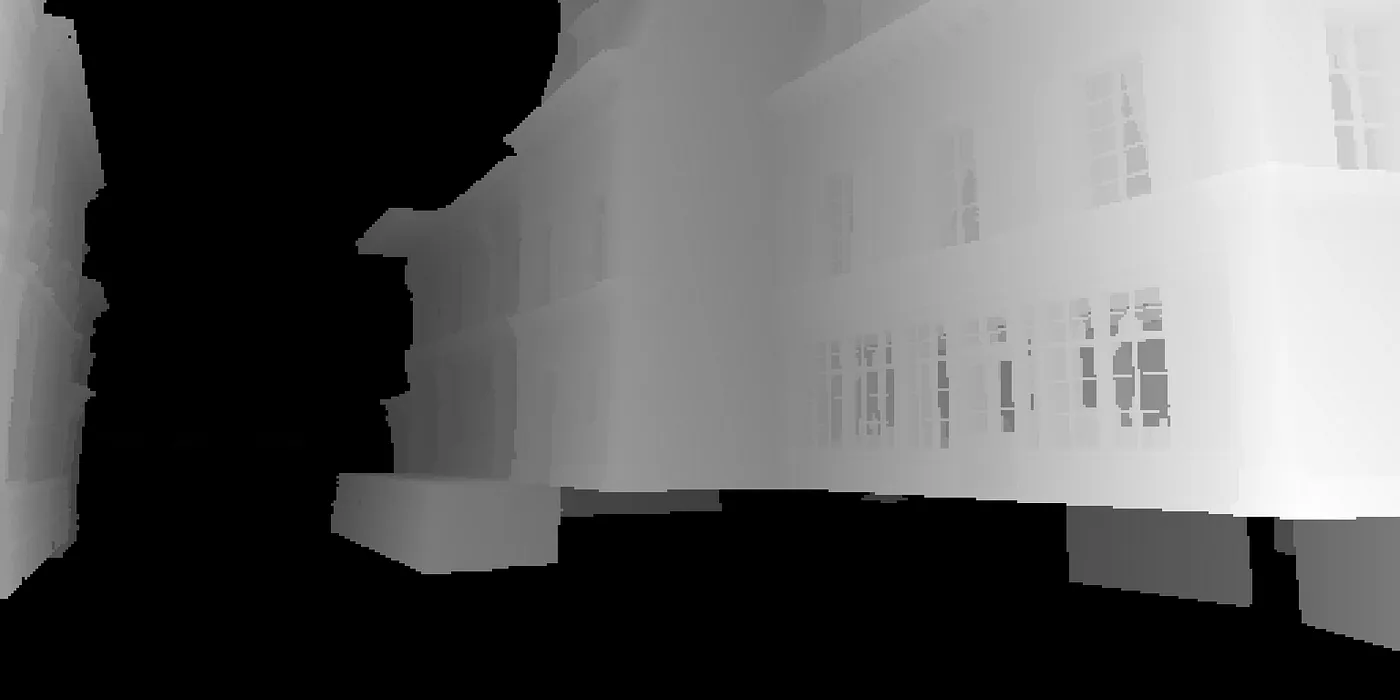
\includegraphics[width=200px]{images/graphics/depth-buffer-ac-unity.png}
    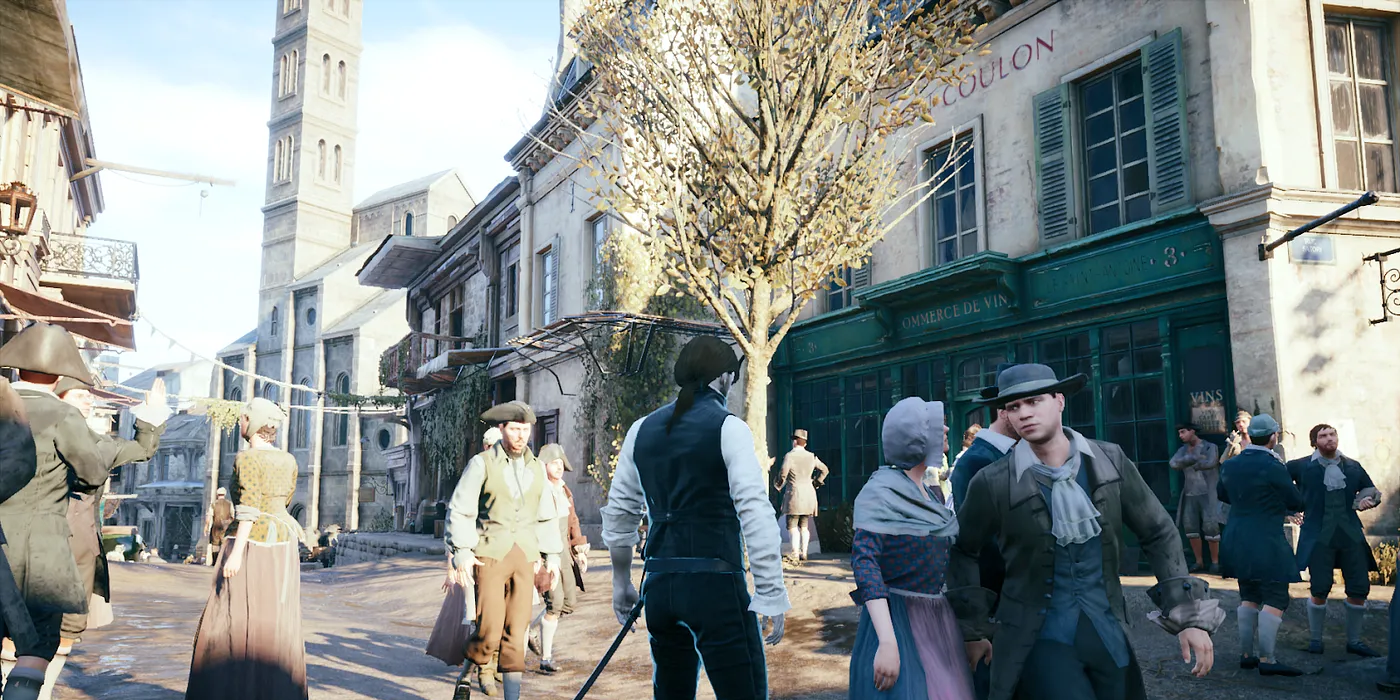
\includegraphics[width=200px]{images/graphics/final-frame-ac-unity.png}
    \caption{The depth buffer (left) and the final back buffer (right) of \emph{Assassin's Creed Unity} (Ubisoft, 2014 \cite{Ubisoft2014}). 
    The hand-picked \emph{best occluders} were already drawn to the depth buffer in a depth pre-pass.
    While rendering all the geometry to the back buffer, each instance can be checked against the z-pyramid \cite{Kruskonja2022}.}
    \label{fig:depth-buffer-ac-unity}
\end{figure}

\noindent
\emph{\ac{TPOC}} is an adaptation of the \ac{HZB} algorithm, introduced in chapter \ref{subsec-hierarchical-z-buffering}. 
One of the most renowned examples of this algorithm is present in the 2014 title \emph{Assassin's Creed Unity} by Ubisoft 
\cite{Ubisoft2014}. One year later, Ulrich Haar and Sebastian Aaltonen presented their approach on SIGGRAPH 2015 
\cite{Aaltonen2015}. Their implementation inspired other developers like \emph{Epic Games} for \emph{Unreal Engine 5} 
to adopt similar techniques \cite{Karis2021}. This is the algorithm we use in our implementation. It shares its basic 
principle with \ac{HZB} but focuses on a more \ac{GPU}-driven configuration and using a given set of best occluders to 
cull instances effectively. \\

\noindent
Some use cases are especially well suited for \ac{TPOC}, \emph{Assassin's Creed Unity} for example has a large open 
world in a city with many large buildings. A rather large amount of instances can therefore be expected to be occluded 
by some of the buildings at any given moment. \ac{TPOC} thus uses artist-picked \emph{best occluders} for \ac{HZB} 
computation. The best occluders are identified during runtime, drawn to depth buffer during a depth pre-pass, and 
then used as described in chapter \ref{subsec-hierarchical-z-buffering}. The output of the depth buffer pre-pass is 
shown in figure \ref{fig:depth-buffer-ac-unity}. Depth passes can be done quite efficiently, especially if they 
only contain a handful of instances to draw. Additionally, because of the advances in \ac{GPU}-driven Rendering, the 
\ac{HiZ} pyramid can be computed by a \emph{compute shader}, which leverages the highly parallel computation 
capabilities of the \ac{GPU}. \\

\noindent
In contrast to the basic \ac{HZB}, this approach relies on the heavy use of \ac{GPU} computation and the pre-
determination of best occluders. This way, the scene doesn't have to be reversed in a front to back order and 
not necessarily needs to incorporate an octree, as long as object bounds can be computed efficiently enough.
In SIGGRAPH 2015 presentation, Aaltonen et al. \cite{Aaltonen2015} mention the addition of another acceleration 
technique, which is compatible with \ac{TPOC}, \emph{Depth Reprojection}.


\subsection{Depth Reprojection} \label{subsec-depth-reprojection}

\emph{Depth Reprojection} makes use of the temporal coherence of the z-buffer. The assumption is made that 
between two consecutive frames most of the visible content remains the same. It is obvious that this will 
hold true for the most part when the camera's rotation and position isn't changed inbetween frames. In this case, 
the last frames depth, color and visibilty information would remain nearly identical. The only differences would 
be introduced by animation or physics simulation, which could move instances independently from the camera movement.
But even with the camera moving over frames, a large part of the scene - static parts like buildings or terrain in 
particular - would retain a lot of its information. This means that there will be a significant coherence in 
visibility between frames, which Depth Reprojection makes use of.\\

\noindent
The algorithm stores the last frame's depth information and "reprojects" it onto the new frame. In the best case, 
most instances, which were previously visible remain visible in this new frame, and instances, which were invisible 
in the previous frame remain invisible in the new frame as well. The new camera transformations and a 
\emph{Velocity Vector Buffer} are used to calculate the delta relative to the previous frame and create an 
approximation of the new depth buffer. Because the reprojected depth buffer is only an approximation, visibility 
and depth calculations can be inprecise, because the result is non-conservative. This means that the reprojection 
process sometimes fails to compute the correct depth values for objects, especially if they move relative to the 
camera. Another problem occurs in use cases, where the camera moves very fast relative to the environment. In such 
a case, the camera might cover a too large distance, so that none of the visible instances in a given frame were 
visible during the previous frame. \cite{Kruskonja2022} \\

\noindent
The \ac{TPOC} algorithm is used in our approach, with minimal changes to the selection of best occluders.
Depth Reprojection could in general be used as well, but is not within the scope of our implementation.

\section{Mesh Shading}  \label{sec-mesh-shading}

Mesh Shaders were first introduced to NVIDIA Turing \ac{GPU}s in 2018 as a part of "a new programmable 
geometric shading pipeline" and built upon the compute programming pipeline \cite{Kubisch2018}. 
Therefore, they aim to optimize work by using the available hardware more efficiently. Compared to the 
traditional vertex shading pipeline, mesh shading introduces a more holistic and parallel processing of 
geometry data. It is incorporated into the rasterized rendering pipeline and has since been used in modern 
gaming. It gained a lot of attention when it was used as the foundation of Epic Games' \emph{Unreal Engine 5} 
feature \emph{Nanite} \cite{Karis2021}.\\

\subsection{The Mesh Shading Pipeline} \label{subsec-the-mesh-shading-pipeline}

In contrast to the \emph{Mesh Shading Rendering Pipeline}, the "traditional" \emph{Vertex Shading Pipeline} 
has more specialized stages, which are listed in figure \ref{fig:traditional-rendering-pipeline}. This pipeline 
is composed of fixed, programmable and optional stages, where each stage operates on some input data and in 
some cases produces output data for the next stage to consume.\\

\begin{figure}[h]
    \centering
    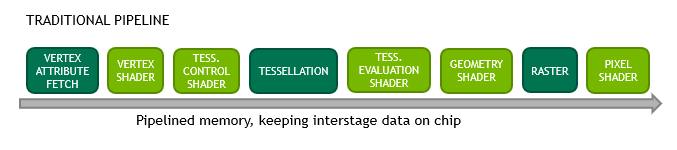
\includegraphics[width=\linewidth]{images/graphics/traditional-rendering-pipeline.png}
    \caption{The traditional rendering pipeline as presented by NVIDIA in \cite{Kubisch2018}.}
    \label{fig:traditional-rendering-pipeline}
\end{figure}

\noindent
The \emph{Vertex Attribute Fetch} stage (also called \emph{Input Assembler} stage) collects the geometric 
input and creates primitives out of it, reading all necessary data associated with the primitive data. 
These primitives are usually triangles but this can vary slightly from use case to use case, depending
on the prior configuration of the stage. After the Input Assembler, the data is sent to the \emph{Vertex Shader}.
This stage is responsible for operating on single vertices, transforming vertices according to the given 
transformation matrices. After that, the \emph{Tesselation Control Shader} can optionally increase geometric 
resolution or triangulate polygonal geometry by applying tesselation functions. The next stage is the optional 
\emph{Geometry Shader}, which is capable of generating additional primitives on the \ac{GPU}. However, it is 
commonly said to be not very efficient and is treated as deprecated since the introduction of the more general 
purpose and faster \emph{Compute Shaders} [@TODO: source]. The three-dimensional scene is then projected onto the 
view plane and is subsequently processed by the \emph{Rasterizer} which samples the continuous lines and faces to 
find the appropriate pixels covered by the geometry. Finally, the final frame buffer is colored correctly by the 
\emph{Pixel Shader}. This stage takes all given parameters like light position, light color, light intensity, camera 
position, vertex colors, textures and many more into account and creates a final, colored image. The pixel shader can 
implement different functions (\ac{BRDF}) for calculation of the final pixel color and is called once per pixel. 
This means, that the computational cost increases with the amount of pixels, i.e. the frame buffer's resolution. 


\begin{figure}[h]
    \centering
    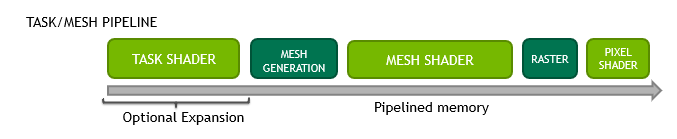
\includegraphics[width=\linewidth]{images/graphics/mesh-rendering-pipeline.png}
    \caption{The mesh shading pipeline as presented by NVIDIA in \cite{Kubisch2018}.}
    \label{fig:mesh-rendering-pipeline}
\end{figure}

\noindent
The \emph{Mesh Shading Rendering Pipeline} is a rendering pipeline, optimized for high geometrical 
density. It shares the Rasterizer and the Pixel Shader stages with the Vertex Shading Pipeline but 
introduces two new stages which aim to replace the Vertex Shader, Geometry Shader and Tesselation stage.
The new stages are called \emph{Task Shader} (or \emph{Amplification Shader}) and \emph{Mesh Shader}. Both 
are fully programmable and are based on the compute shader architecture. Therefore, they are inherently different 
from the traditional Vertex Shader stage, even though they both can be used for vertex transformations.
Figure \ref{fig:mesh-rendering-pipeline} shows the pipeline stages and the order they are executed in. \\

\noindent [@TODO: Check redundancy in first two sentances]
The Task Shader serves as a precomputational stage which is optional and invokes the Mesh Shader.
It can take any arbitrary data as input and operates on the provided data to produce output data, which in 
turn is scheduled for execution on the Mesh Shader. Since both shaders are based on compute shaders, a thread 
group size can be specified and groupshared memory can be allocated. This allows for highly parallelized execution 
and optimized memory usage. A key difference to the traditional pipeline is that the Amplification Shader can 
invoke other compute shaders, create new tasks and dispatch none, one, or multiple mesh shader invocations. This 
makes the shader extremely flexible and capable of providing the same results as the Geometry Shader does, but 
faster and more scalable.\\

[@TODO: Add picture of meshlets]
\noindent
The Mesh Shader output can be defined individually but usually it creates a small patch consisting of a small 
number of triangles, called \emph{Meshlet}. This new approach to operate on vertices allows for a new interpretation 
of mesh data. The primitive topology is not anymore constrained to triangles, triangle fans and triangle strips, 
but can be individually specified by the developers.
Meshlets are computed by thread groups which usually fetch the mesh data from the given vertex and index buffers and 
apply transformations and arbitrary operations. This new way of processing geometry is not only more efficient in many 
cases and reduces the memory bandwidth, but also allows for per-meshlet operations \cite{Kubisch2020}. This is a key 
advantage, since per-instance geometry can now be processed in parallel and still be individually discarded or post-processed. 
There are several other advantages over the traditional Vertex Shaded Pipeline, which we will not list to the full 
degree. More details are provided in the blog post by NVIDIA \cite{Kubisch2020}.\\


\subsection{Meshlet Culling} \label{subsec-meshlet-culling}

One major innovation that is enabled by the use of Mesh Shading is to cull on a per-primitive (per-meshlet) basis. 
This allows for more granular culling of high density geometry even within instances. Prior to the implementation 
of meshlets, culling usually was done on a per-instance basis (or for backface culling on a per-triangle basis), 
omitting whole instances depending on their position in space or their visibility from the point of view of the camera.\\

\noindent
But although the Mesh Shading Pipeline was first introduced in 2018, the idea of triangle clusters goes back even further.
One example of this \ac{GPU}-driven rendering technique is the 2014 title \emph{Assassin's Creed Unity} \cite{Ubisoft2014}.
Aaltonen et al. \cite{Aaltonen2015} provide an overview over multiple cluster related optimization techniques, implementing 
a highly parallelized rendering pipeline before Mesh Shading became part of the official Rendering \ac{API}s.
For their \ac{GPU} culling algorithms they refer to the prior work of Hill \cite{Hill11} and Greene \cite{Greene93}, which 
provides the basis for some of the implementation in our case study. Most of the culling algorithms discussed in chapter 
\ref{sec-culling-techniques} can be adopted to use meshlet culling. The algorithms can usually be applied to triangle clusters 
without the need of changing a lot of the algorithm. Bounding volumes can be calculated for meshlets, too, and meshlets do also 
consist of triangles themselves. In this chapter we briefly revisit the basic culling algorithms and show, how they can be 
adapted for the Mesh Shading pipeline.

\subsubsection{Meshlet Backface Culling} \label{subsubsec-meshlet-backface-culling}

As shown in chapter \ref{subsec-backface-culling}, there are backface culling algorithms which can be applied to 
triangle clusters as well. For instance, the normal cone approach by Shirmun et al \cite{Shirmun1993} can be used 
in the Mesh Shading pipeline as well. In fact, having a hardware and software support for the computation of triangle 
clusters makes this approach even more efficient. Clusters are evaluated in parallel, making a normal cone backface 
culling algorithm very fast. \\

\noindent
Another algorithm compatible with triangle clusters is the one propsed by Aaltonen et al. \cite{Aaltonen2015}, again 
in the context of the SIGGRAPH 2015 presentation, showing their work for \emph{Assassins Creed Unity}. They introduce 
a small bounding cube around \emph{n} triangles, which could correspond to a meshlet in the Mesh Shading pipeline. 
"Each cube face is split into \emph{r} \begin{math}\times\end{math} \emph{r} 'pixels', each encoding an \emph{n}-
bit mask that indicates whether the corresponding triangle is visible over that 'pixel'" \cite{AkenineMoeller2018}.
As long as the camera is outside of the cube, the center of the cube creates a frustum with any of the "pixels" on 
the cube's surface, as shown in figure \ref{fig:backface-culling-ac-unity}. The frustum in which the camera is 
located can be found and the bitmask can be accessed. This way, the backfacing triangles can be identified and 
culled. \cite{Aaltonen2015}, \cite{AkenineMoeller2018}

\begin{figure}[h]
    \centering
    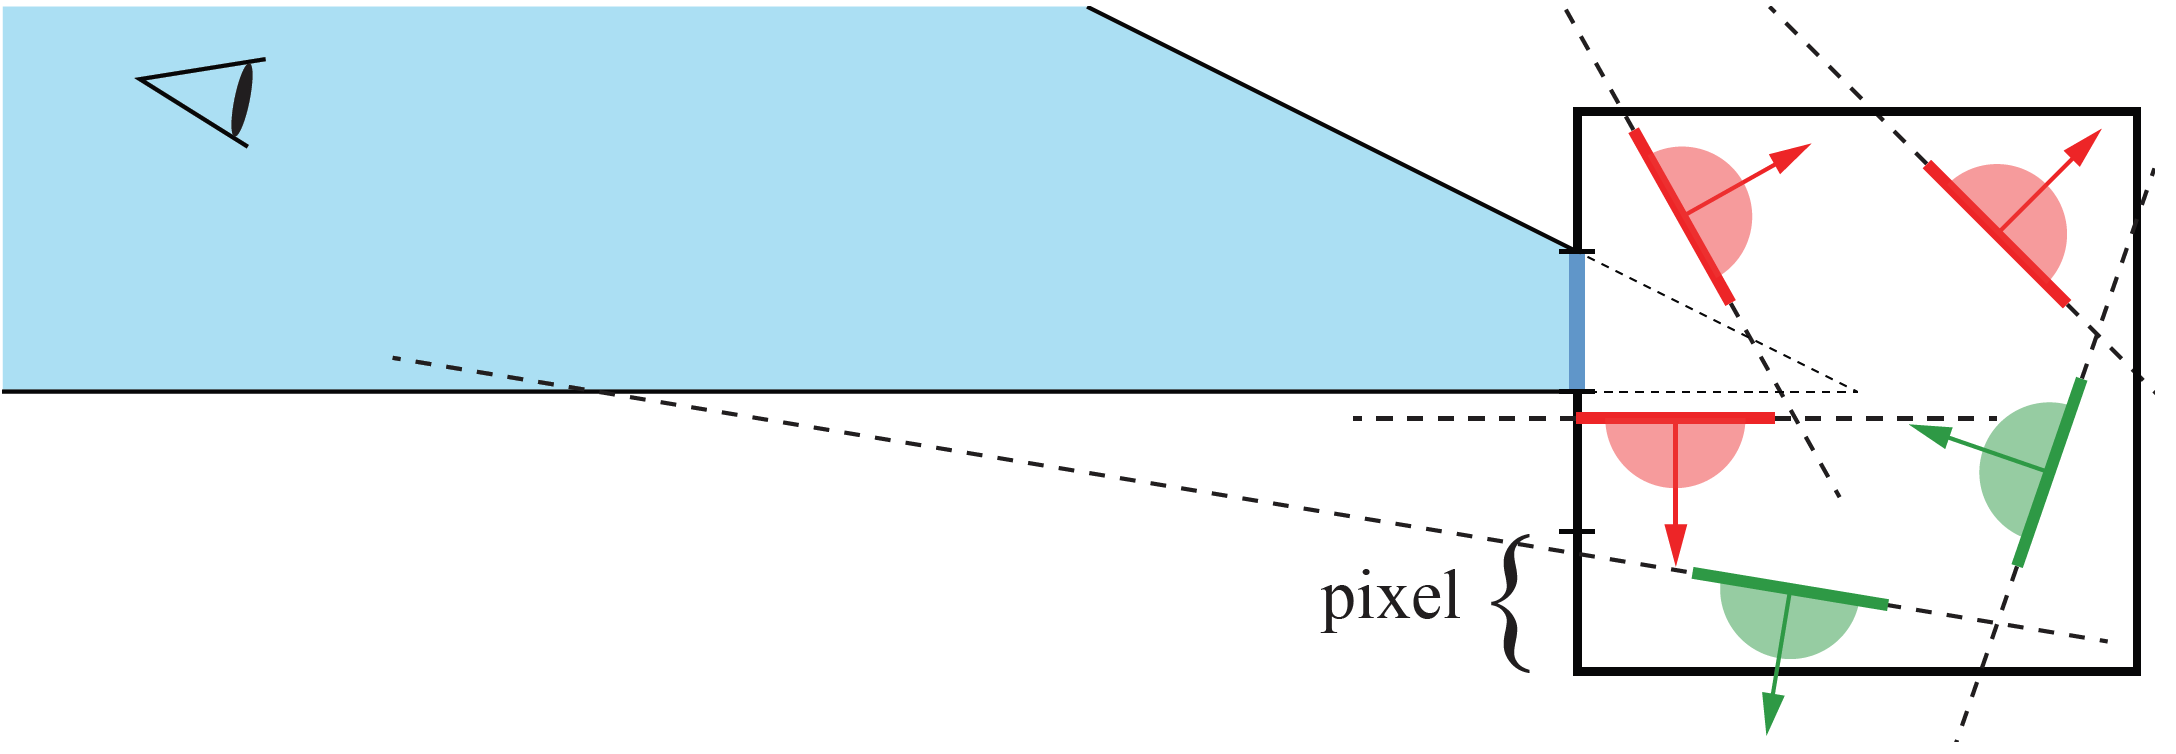
\includegraphics[width=\linewidth]{images/graphics/backface-culling-ac-unity.png}
    \caption{Backface culling thechnique using a bounding box around a set of \emph{n} triangles, 
    as proposed by Aaltonen et al. \cite{Aaltonen2015}. Image by Akenine-Möller et al. \cite{AkenineMoeller2018}.}
    \label{fig:backface-culling-ac-unity}
\end{figure}


\subsubsection{Meshlet View Frustum Culling} \label{subsubsec-meshlet-view-frustum-culling}

[@TODO: Check if pre-calculated meshlets have been introduced; find sources]
Frustum culling can be adapted to work on meshlets as well. Similar to backface culling, the basic technique remains 
the same, but is applied to triangle clusters (meshlets) rather than instances (meshes). To implement this, meshlet 
bounding volumes need to be computed. The same principles apply to meshlet bounding volumes as to instance bounding 
volumes, so spherical volumes are usually fast and cheap to calculate. If the meshlets are pre-calculated, the 
bounding volumes can be precalculated as well, since they will not change over time. Then, frustum culling is as simple 
as using any existing frustum culling algorithm (see \ref{subsec-view-frustum-culling}) and applying it to the meshlets.
Since this can be done in the Task Shader, the culling can be computed in parallel and culled meshlets can be discarded 
early. This includes parts of single instances, which allows for even better optimization. In the traditional Vertex 
Shading pipeline, instances had to be completely outside of the view frustum in order to be culled. If an instance is 
partially visible in the Mesh Shading pipeline, the meshlets inside the frustum can be drawn and the meshlets outside 
of the frustum can be discarded. \\

\noindent
We use view frustum culling of individual meshlets in our approach to further optimize performance. A simple 
implementation was already included in the framework we used for our case study.

\subsubsection{Meshlet Occlusion Culling} \label{subsubsec-meshlet-occlusion-culling}

Meshlet occlusion culling refers to the process of culling meshlets which are occluded by any other meshlet, by a 
group of meshlets or another instance. This culling technique is rather new due to the relative novelty of the 
Mesh Shading pipeline itself. Still, Aaltonen et al. \cite{Aaltonen2015} used what they call \emph{Cluster Culling} in 
\emph{Assassin's Creed Unity} (Ubisoft \cite{Ubisoft2014}, 2014). Meshlet occlusion culling can be implemented in 
a bunch of different ways, exactly as traditional occlusion culling algorithms. Often, this implies the use of a 
\ac{BVH} like an octree to make visibilty checks easier. \ac{HZB} can also be applied to the new pipeline, and meshlets 
can be checked for occlusion, using the highly parallel Mesh Shading pipeline. Consequently, \ac{TPOC} is also applied 
to individual meshlets, as seen in Alan Wake 2 (Remedy Entertainment \cite{Remedy2023}, 2023) or Epic Games' 
\emph{Unreal Engine 5} and \emph{Nanite} \cite{Karis2021}.\\

\noindent
We believe that this new way of culling single meshes can generate new innovation in the field of computer graphics.
This is why we decided to implement our approach in a Mesh Shading pipeline, which, when used carefully, is more 
efficient than comparable methods like the use of Geometry Shaders or Instancing.
    \chapter{Implementation} \label{cpt-implementation}

The implementation used for the experiment is based on an implementation within the framework \emph{Diligent Engine} 
\cite{DiligentGraphicsGitHub, DiligentGraphics}. This framework includes a rendering backend supporting 
multiple rendering \ac{API}s, with integrations for modern \ac{GPU}-driven rendering, such as the support for 
mesh shading in Microsoft's D3D12 rendering \ac{API}. The support for modern rendering features, while still 
maintaining access to all core features, makes \emph{Diligent Engine} a good place to start from.\\

\noindent
For the experiment, the Mesh Shading pipeline is enhanced to better fit the purpose of drawing a huge amount of voxels. 
Also, the integrated view-frustum culling was altered to some degree so that it works on meshlet-groups rather 
than meshlets themselves. This change was made during the restructuring of the draw tasks. The updated pipeline 
changes how meshes are dispatched because of the use of additional acceleration structures. This chapter provides 
a detailed overview of the complete pipeline and how it works in particular. The full implementation details can be 
found in appendix \ref{cpt-appendix}.

[@TODO: Add meshlet based view frustum culling impl is used and was already in Diligent Engine]

\section{Pipeline Initialization} \label{sec-piepline-initialization}

\begin{figure}[h]
    \centering
    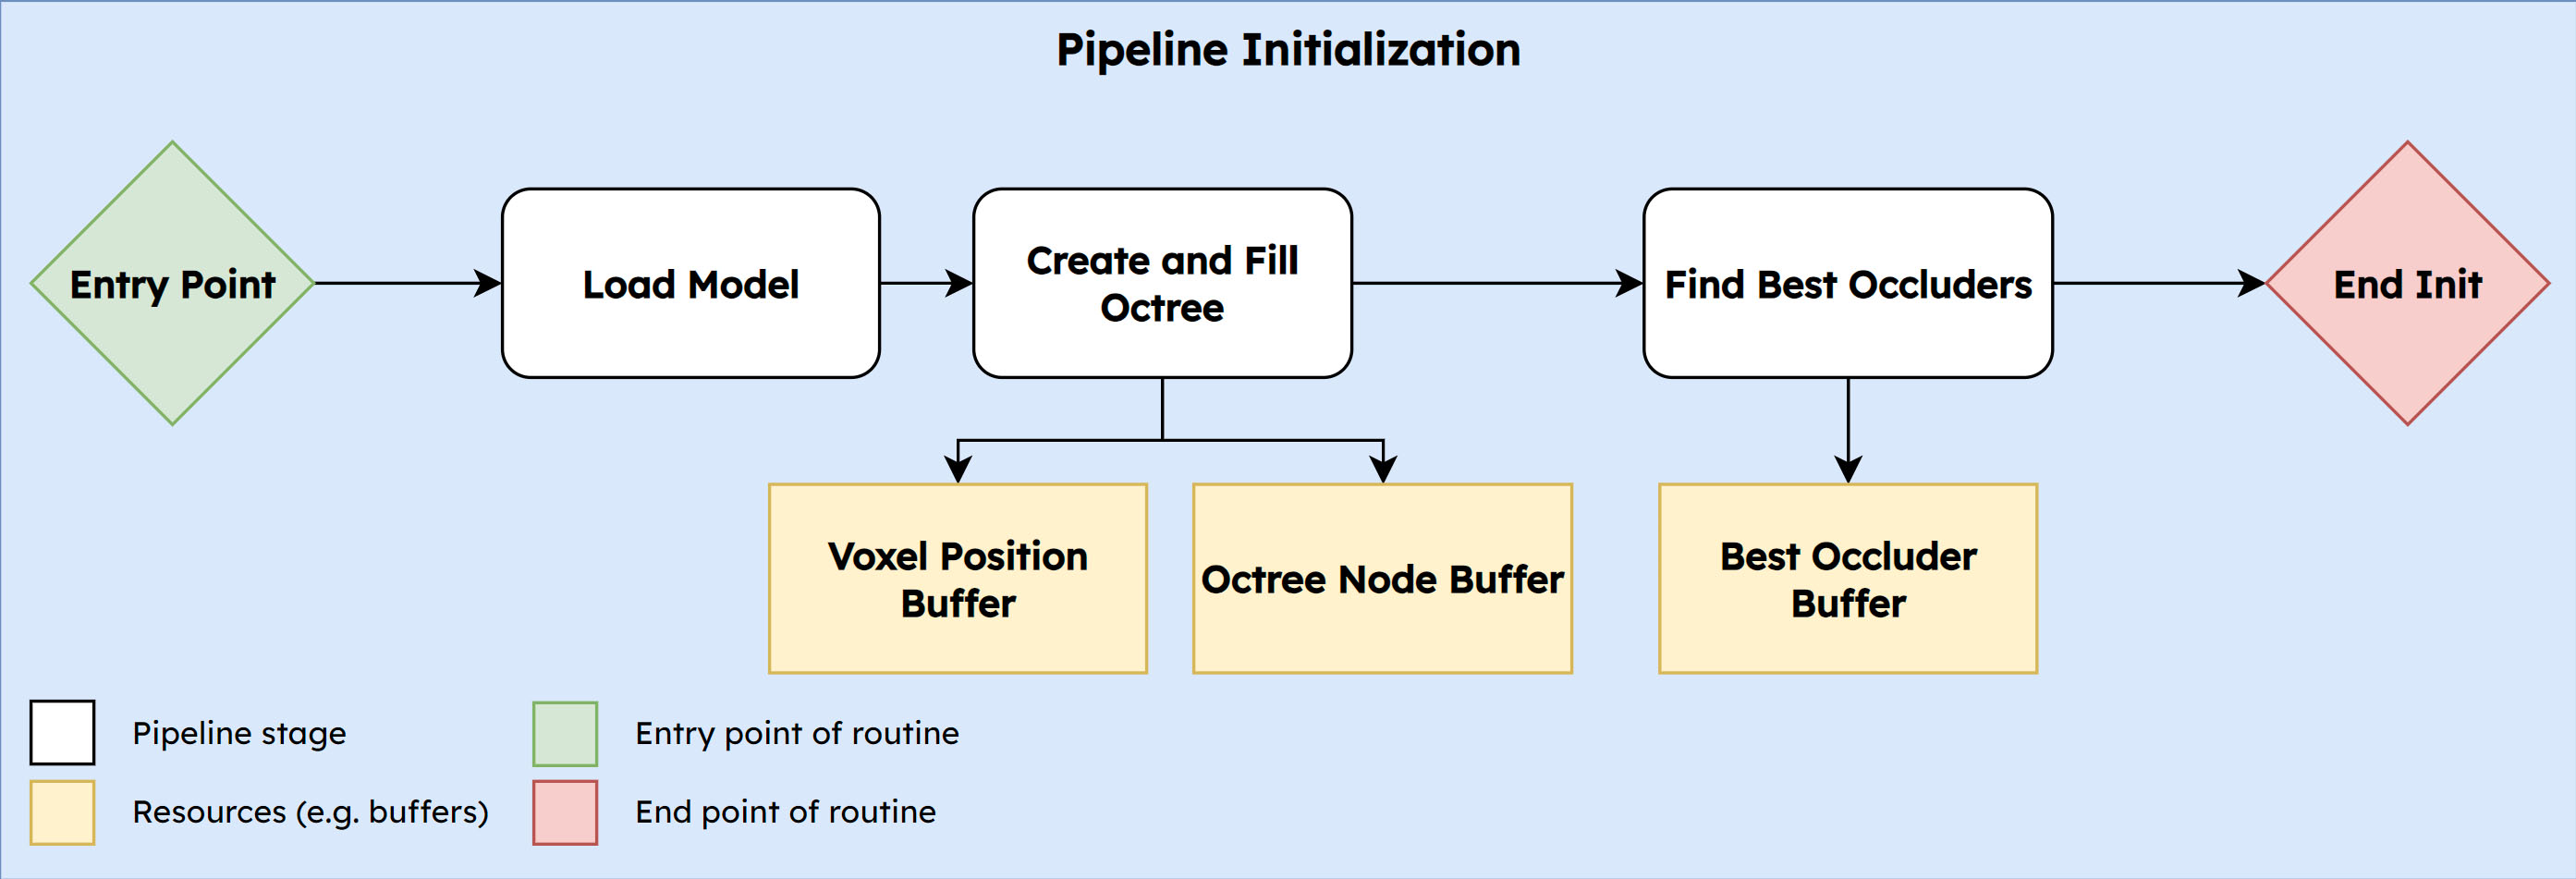
\includegraphics[width=\linewidth]{images/graphics/pipeline-initialization.jpg}
    \caption{The initialization process of the rendering pipeline. Depending on the voxel model, an octree node 
    can hold anything between zero and \emph{n} voxels, \emph{n} being the amount of threads per threadgroup.}
    \label{fig:pipeline-initialization}
\end{figure}

\noindent
The pipeline is split into an initialization routine and an update loop. The initialization is called once during 
the beginning of the execution flow, and the render loop is initiated after the initialization is finished. Then, 
the loop is called each frame. Figure \ref{fig:pipeline-initialization} shows the initialization procedure. 

\subsection*{Voxel Model Loading} \label{subsec-voxel-model-loading}

For the purpose of this experiment, a single, solid voxel mesh is loaded, but this could also be a scene 
consisting of multiple solid voxel models. In the provided implementation, the positions of voxels inside a regular 
grid are loaded, skipping grid cells where no voxels are located. For loading the voxels, the tool \emph{binvox} 
is used \cite{binvox, Nooruddin2003}. It is a command-line tool that converts triangle meshes (e.g. \emph{.obj}) to 
a volumetric voxel representation. The resulting file can be consumed by the engine. Figure 
\ref{fig:trimesh-to-voxel-mesh} shows both the triangle mesh and the processed volumetric voxel mesh. 

\begin{figure}[h]
    \centering
    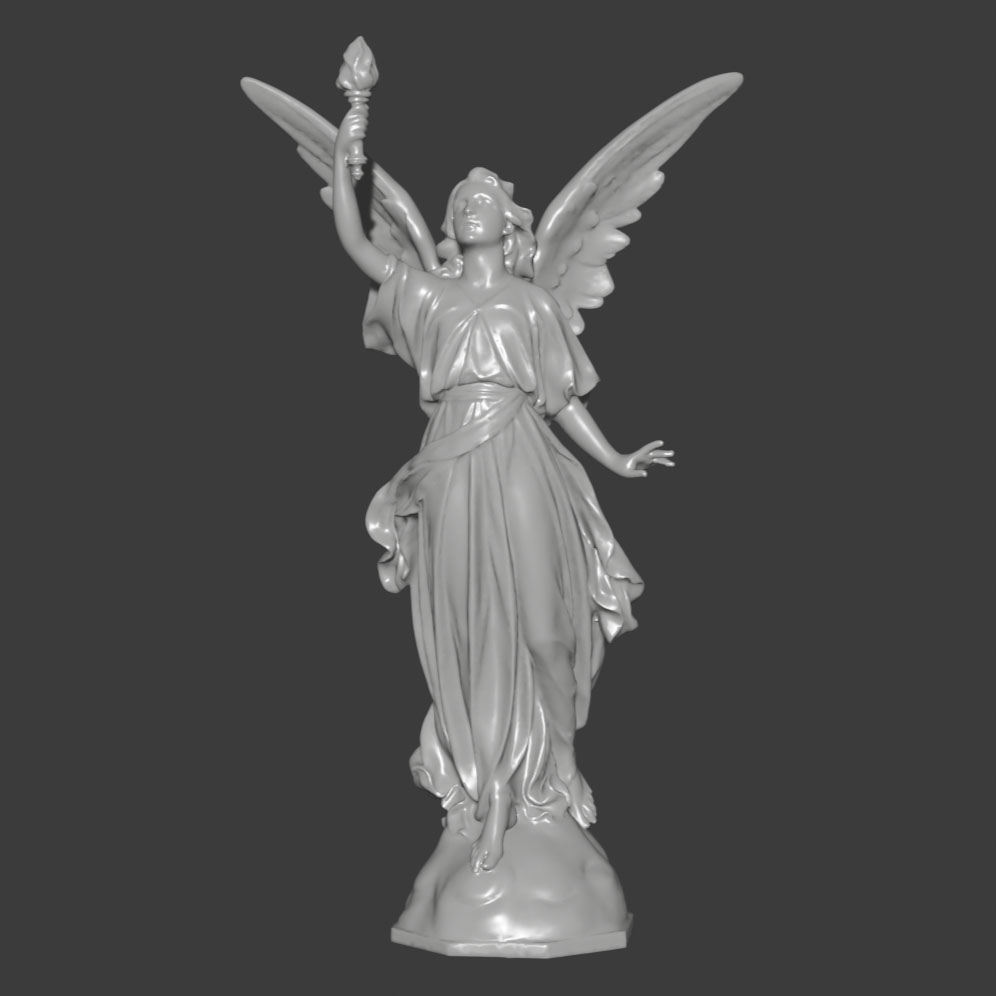
\includegraphics[width=200px]{images/graphics/lucy-triangle-mesh.jpg}
    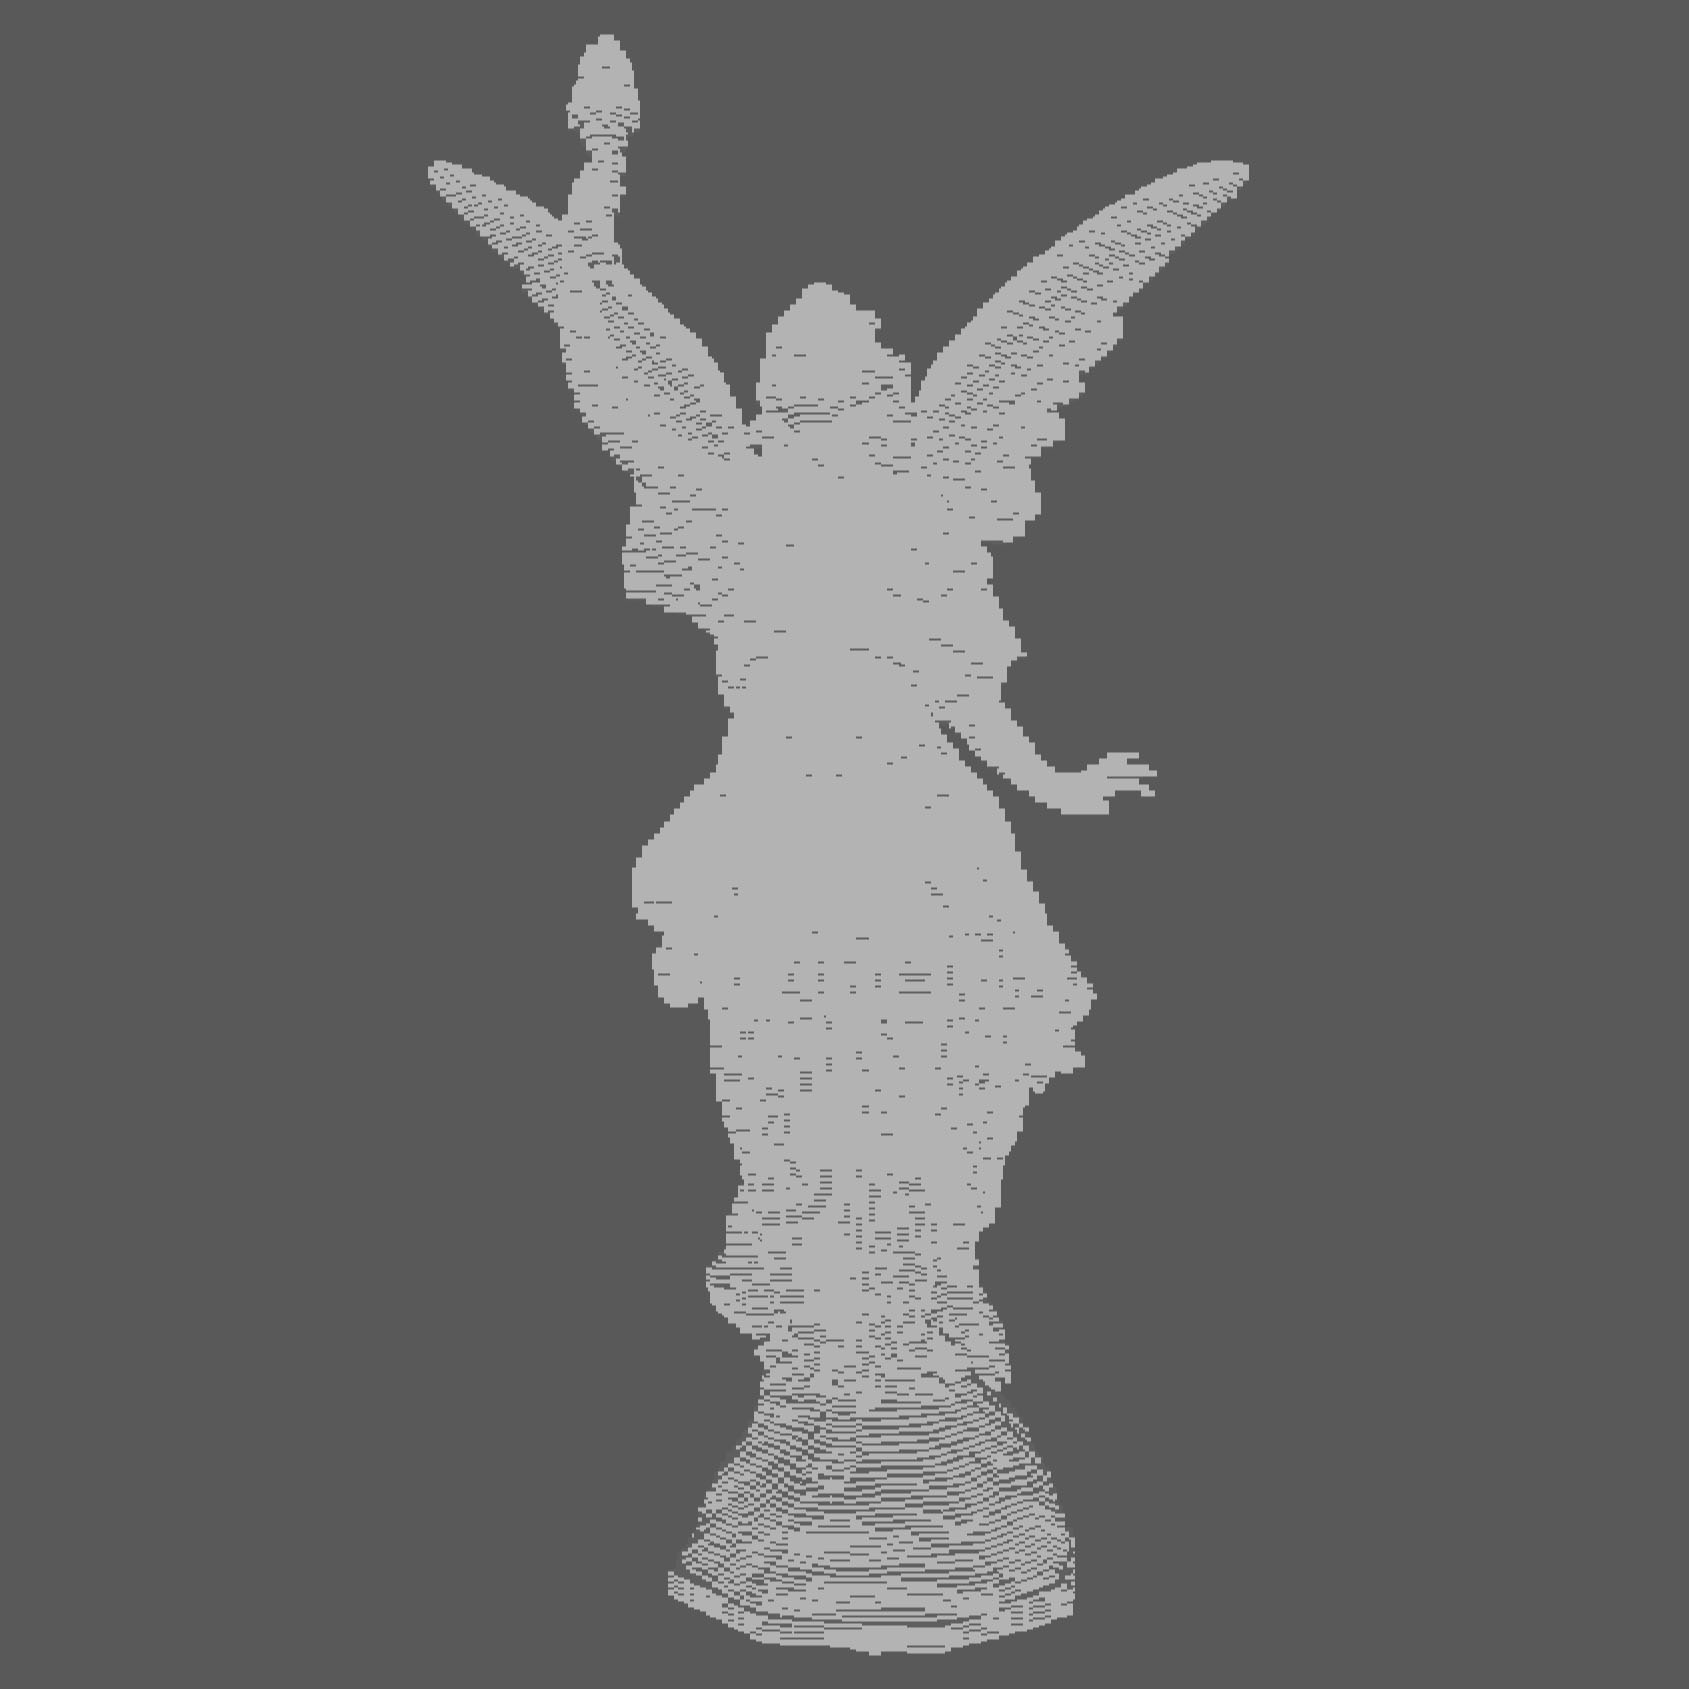
\includegraphics[width=200px]{images/graphics/lucy-voxel-mesh.jpg}
    \caption{The input triangle mesh (left) and the voxelized and parsed voxel mesh (right). 
    Model \emph{Lucy} from \emph{The Stanford 3D Scanning Repository} \cite{Stanford23}.}
    \label{fig:trimesh-to-voxel-mesh}
\end{figure}


\noindent
This model is then processed to fit the requirements of the proposed rendering pipeline. Central to the pipeline 
are the data structures and the \ac{GPU} resources filled with the respective data. To minimize the memory footprint,
the geometry is created on the \ac{GPU}. The only requirement to uniquely identify a voxel then is to know its position.
The main resource is therefore a buffer filled with all the voxel positions as \emph{x, y, z} coordinates. Since \ac{GPU} 
resources usually have to be aligned, 4 bytes of extra space can be used to store the voxel size alongside the position.
It can be used to vary the size of the visible mesh or, for instance, to calculate bounding boxes separately. \\

\noindent [@TODO: Double check because of comparison between both possible implementations]
The voxel positions are already sufficient to render the voxel mesh by making each voxel one meshlet. This means that 
individual voxels can be culled based on various meshlet culling techniques outlined in chapter 
\ref{subsec-meshlet-culling}. Each \ac{GPU} thread generates one voxel, or none if the voxel is found to be culled. 
As long as voxels are computed individually, this is very efficient and keeps the memory usage comparably low. But for 
more sophisticated computations, more data is necessary in order to compute spatial characteristics for the voxels. \\

\noindent
Especially when dealing with a lot of voxels, it can be beneficial to cull groups of voxels. So for the proposed 
implementation, it serves well to manage an octree alongside the voxel position data. This additional data structure 
can be used to interpret the data differently. Now each \ac{GPU} threadgroup computes the voxels of one octree node, 
with the maximum amount of voxels per node being equal to the number of threads per threadgroup. Using this layout, 
each thread in a threadgroup again takes care of at most one voxel. The octree node structure can now store additional 
information that can be used for octree node-based culling.

\subsection*{Octree Creation} \label{subsec-octree-creation}

\begin{figure}[h]
    \centering
    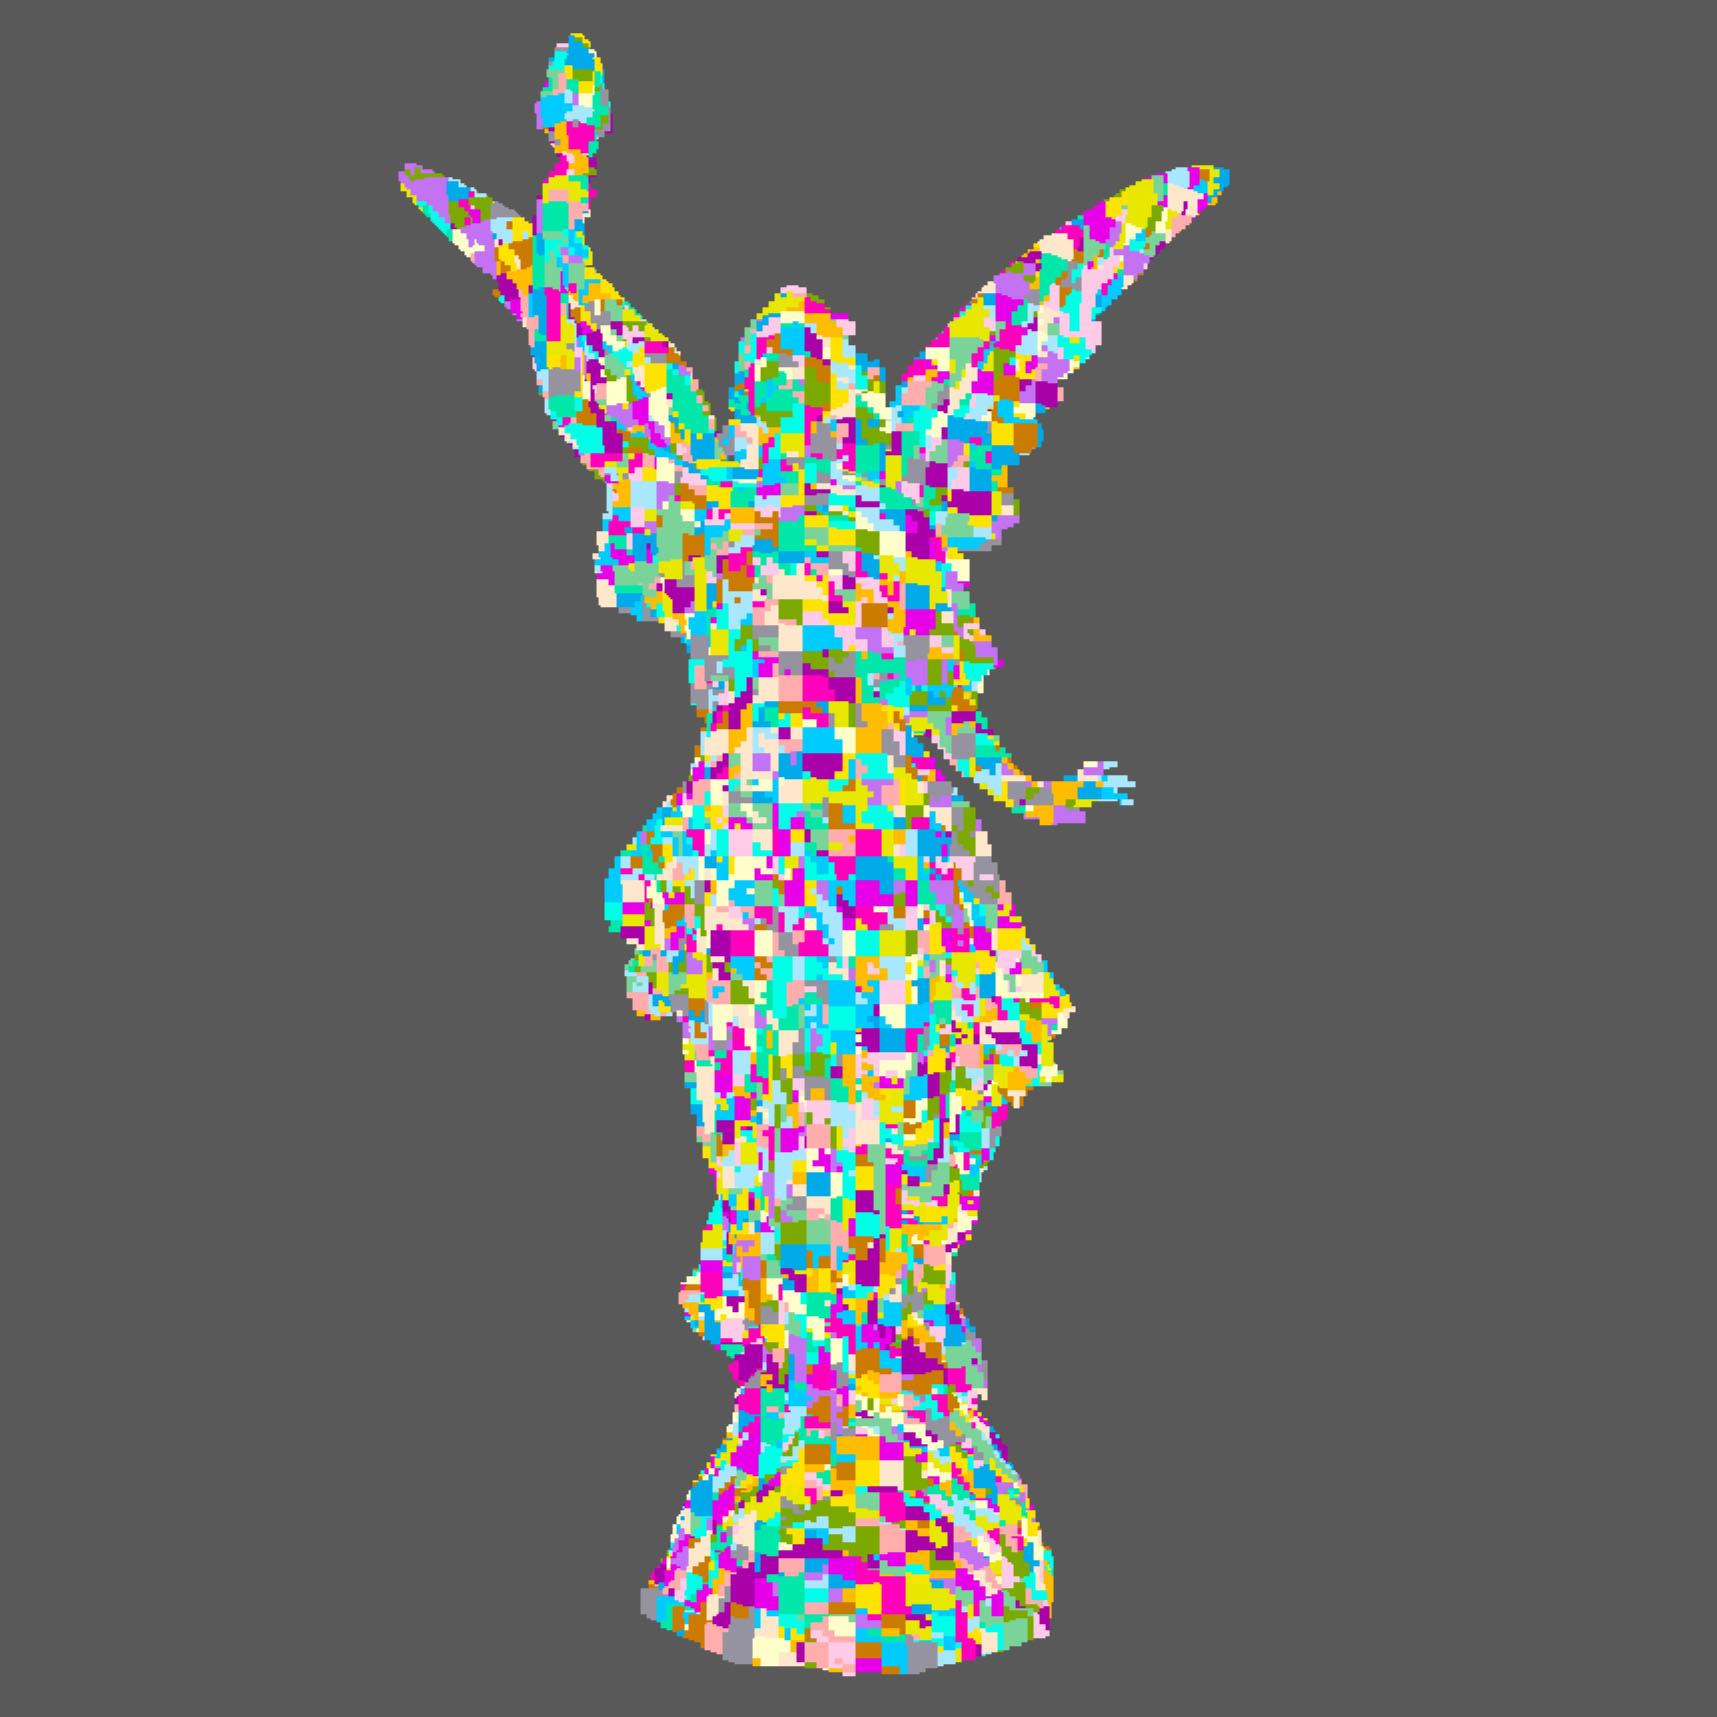
\includegraphics[width=151.5px]{images/graphics/lucy-voxel-octree-viz.jpg}
    
\includegraphics[width=250px]{images/graphics/lucy-voxel-octree-viz-2.jpg}
    \caption{The octree structure visualized. Each color represents one octree node. The whole model contains 
    \emph{470.355} voxels and \emph{19.823} octree nodes, with one leaf octree node holding up to \begin{math} 4 \times 4 \times 4 \end{math}
    voxels.}
    \label{fig:voxel-octree-viz}
\end{figure}

\noindent
After loading any voxel model, an octree is created that covers the entire scene - in the simplest case, there is 
only one model present, so the octree's bounding volume is considered to be equal to the bouding volume of the voxel 
model. As discussed in Chapter \ref{subsec-highres-svo-dags}, it is recommended to use a highly efficient and 
compressed octree implementation like an \ac{SVO} or a Sparse Voxel \ac{DAG} \cite{Kampe2013}. For the purpose of 
this work, a custom octree implementation is used, which refers to indices in the \emph{voxel position buffer}, 
as shown in Figure \ref{fig:voxelpos-octreenode-buffer}. \\

\begin{figure}[h]
    \centering
    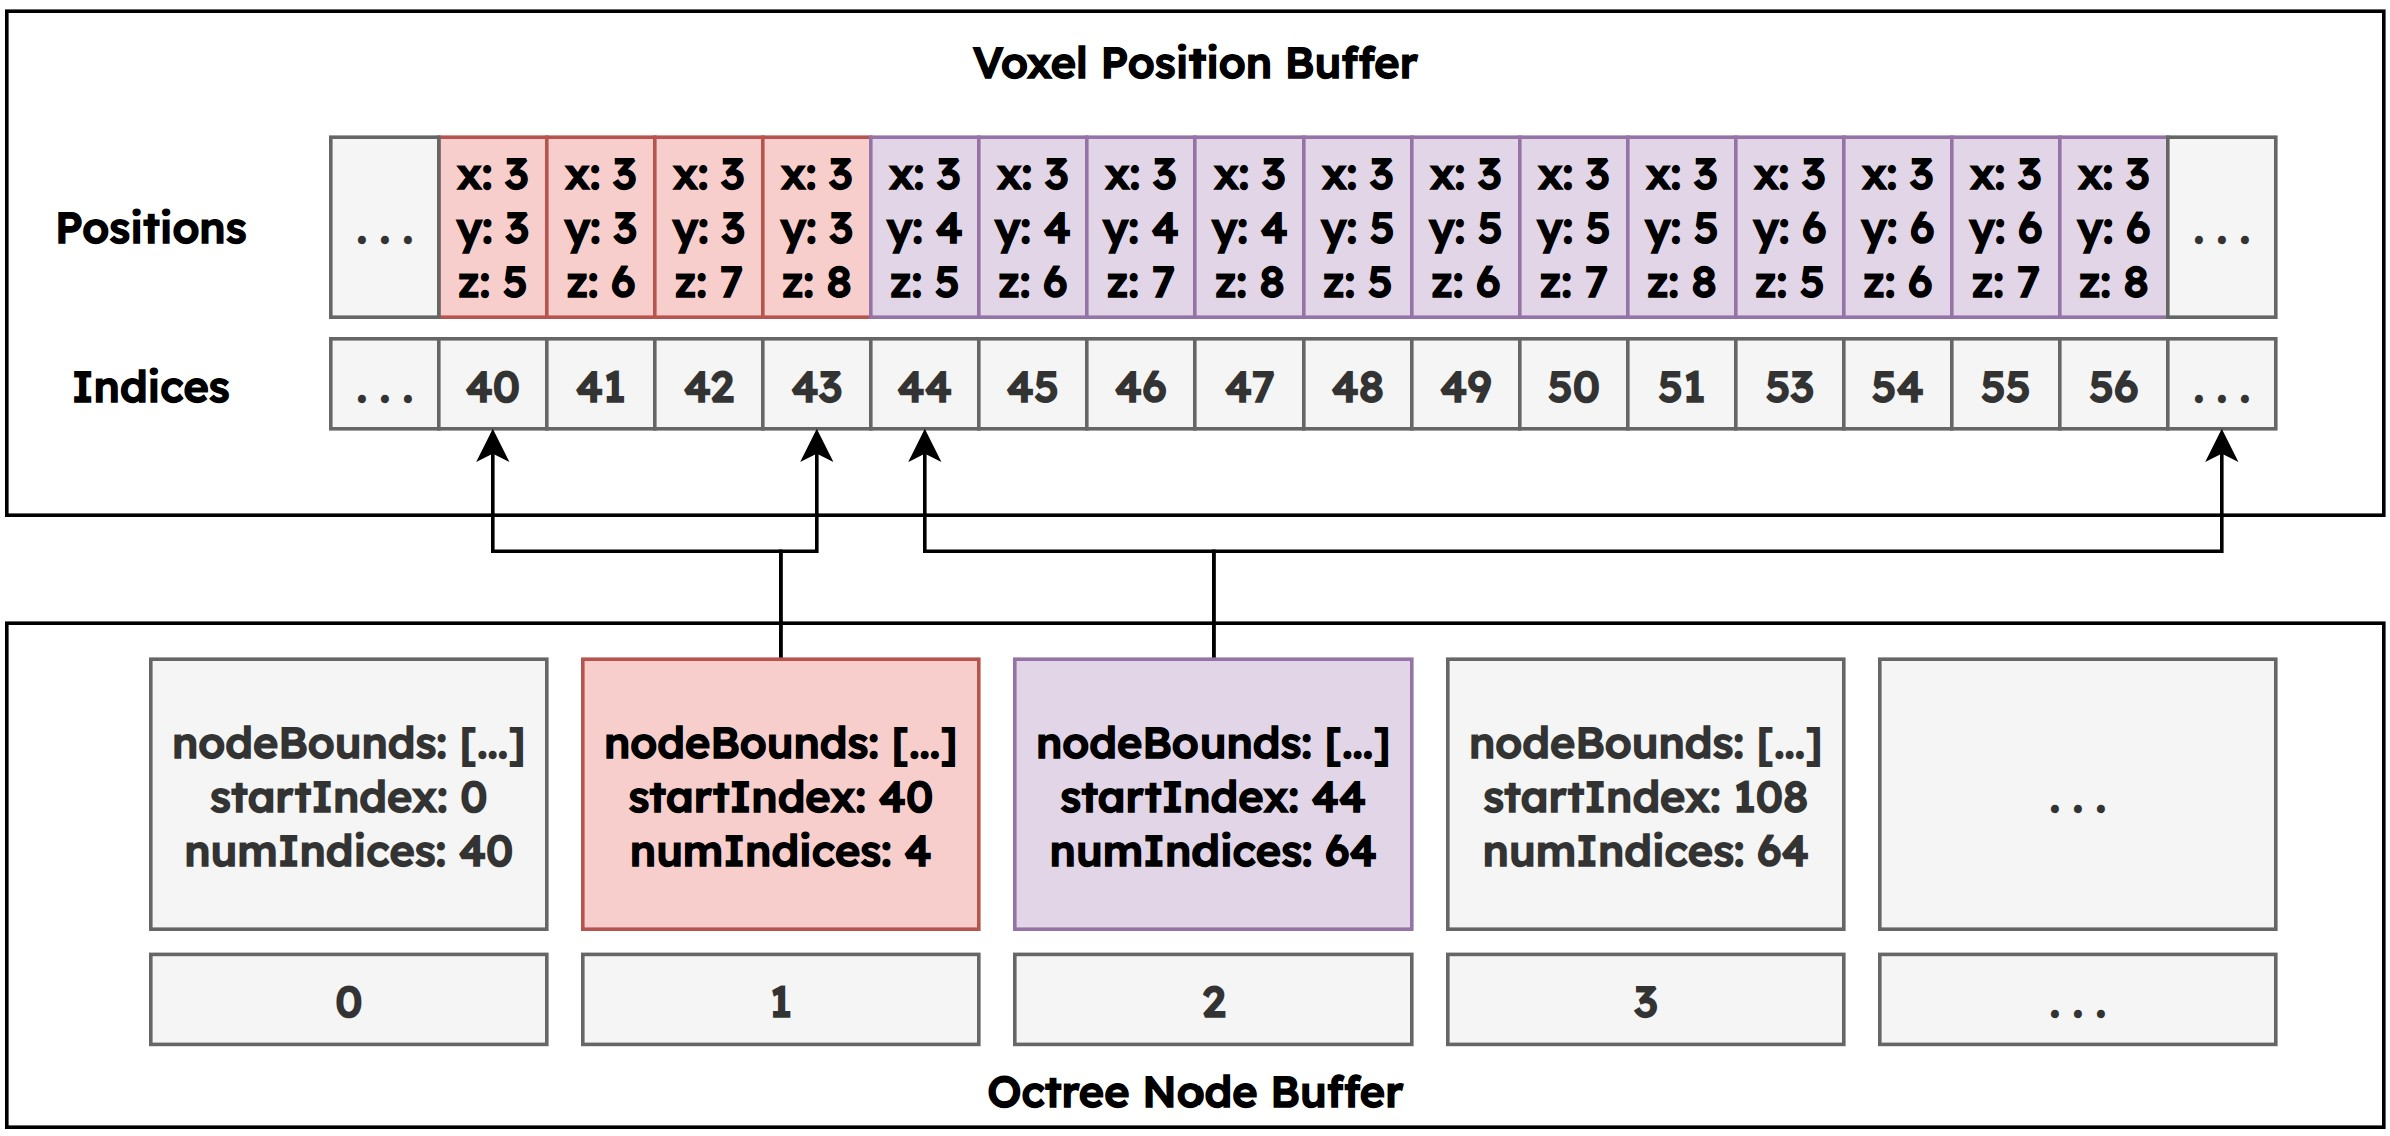
\includegraphics[width=\linewidth]{images/graphics/voxelpos-octreenode-buffer.jpg}
    \caption{The voxel position buffer and the octree node buffer. The latter one providing a 
    specific structure to the first one.}
    \label{fig:voxelpos-octreenode-buffer}
\end{figure}

\noindent
Figure \ref{fig:voxelpos-octreenode-buffer} shows the relation between the octree resource and the \emph{voxel position buffer}.
Since an octree is an inherently hierarchical data structure, it needs to be "flattened" in order to be efficiently fed 
to the \ac{GPU}. This process involves sorting the \emph{voxel position buffer} so voxels within one octree node can be 
located adjacent to one another. The additional "flat" \emph{octree node buffer} then only needs a \emph{start index} 
and a \emph{voxel count} to represent the octree node. Additionally, the octree node's bounds are stored alongside the 
\emph{start index} and the \emph{voxel count}, so octree node-based computations can be executed on the \ac{GPU} side. \\

\noindent
Figure \ref{fig:voxel-octree-viz} shows that the voxels are grouped into octree nodes, which are visualized by distinct 
random colors. 


\subsection*{Best Occluder Selection} \label{subsec-best-occluder-selection}

[@TODO: Evaluate problem of non-static best occluders]
The next step in the initialization procedure is to precompute the best occluders. As mentioned in chapter 
\ref{subsubsec-two-pass-occlusion-culling}, best occluders are usually authored by artists during the creation of 
the scene. This process is only possible if the models are static in the sense that they do not change in size or 
shape. Although a change in position or rotation is not technically a problem, best occluders are usually inherently 
static. Changes to the properties of the occluder could result in inefficient occlusion queries or even the elimination 
of occluders altogether. In the context of volumetric scene representations, this can be a problem since voxel models 
are often a target of manipulation by players or physical interactions. So a predetermination of best occluders is not 
possible in the way it is for static models. This specific scenario is what the presented approach aims for and why the 
next step in the pipeline preprocesses best occluders. Note that this implementation does not include an update of 
the best occluders. It only serves as an experiment of the occlusion culling algorithm in the context of voxel rendering. 
Updating the best occluders when the voxel model is altered needs to be evaluated separately, but is considered to be 
viable for occasional changes to the mesh. A more demanding change to the octree content is given when computing physical 
interactions within the duration of a frame. In this case, further tests need to be done to evaluate the impact on 
performance. \\

\noindent
The provided approach makes use of the inner, non-visible voxels and approximates them using the octree. For this 
to work, full octree nodes are used as occluders. This means an octree node is a best occluder if the number of 
voxels present within the respective node is equal to the maximum number of voxels possible in that node. Only full 
nodes can be considered best occluders because their shape can be approximated. If the node is not completely filled 
or has holes in it, the approximation will not work. This property of a best occluder is propagated up the tree, as 
long as all eight child nodes satisfy the requirements of being a best occluder. Figure 
\ref{fig:octreenode-filled-non-filled} shows three possible leaf nodes. 

\begin{figure}[h]
    \centering
    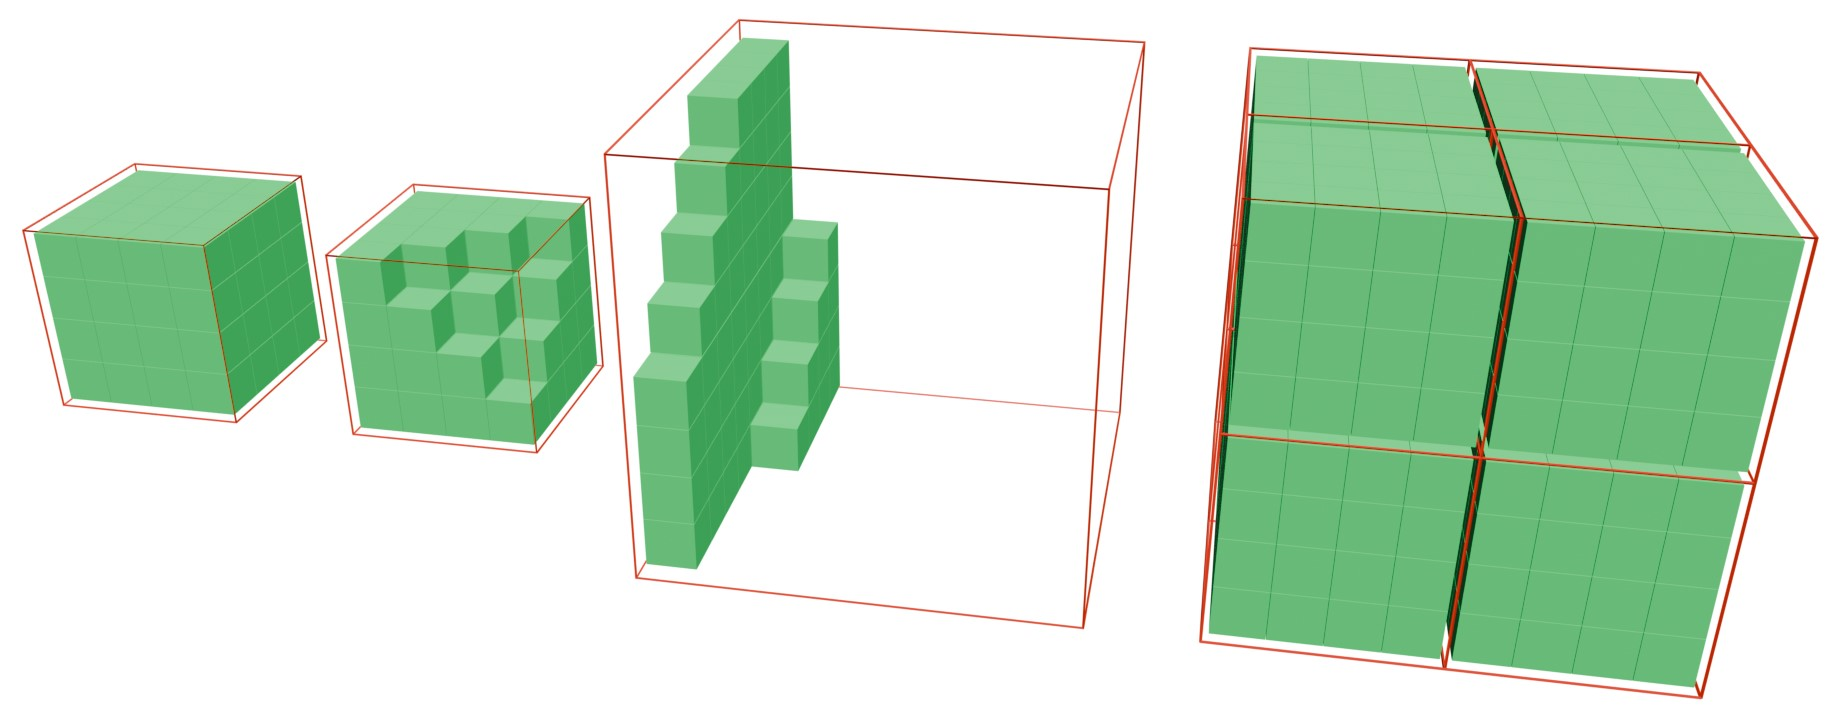
\includegraphics[width=300px]{images/graphics/octree-nodes-filled.jpg}
    \caption{Four possible \emph{octree leaf node} setups. The most left node is completely filled up to its 
    boundary and therefore considered to be a best occluder. The middle left node is not completely filled and therefore 
    not considered to be a best occluder. The middle right node has larger boundaries but can still be a leaf node as long 
    as the amount of voxels in the node doesn't force the node to split. Since it is not completely filled it is not 
    considered to be a best occluder. The right node has eight full child nodes and is therefore considered full and a best occluder.
    The gaps between voxels and the node boundaries are only for visualization purposes.}
    \label{fig:octreenode-filled-non-filled}
\end{figure}

\noindent
During the depth pre-pass, the best occluders are drawn as "large voxels", which are the size of the respective 
best occluder node. This can be achieved by simply reusing the mesh shader used in the normal draw call and 
inputting the node's position and bounds. This way, a whole node gets drawn instead of the individual voxels, 
reducing the computation cost for drawing the best occluders considerably. The best occluders are stored in a 
separate buffer so they can be dispatched efficiently. \\

\noindent
This concludes the initialization of the pipeline. When changes are applied to the voxel data, the voxel buffer,
the octree node buffer, and the best occluder buffer need to be updated accordingly. Alternatively, the best 
occluders can be implicitly calculated on the basis of the octree node buffer. This would make the best 
occluder buffer redundant but would result in a higher dispatch count with a lot of discarded nodes, 
where the criteria for best occluder are not met. Since all computations are more or less in parallel, this 
will not affect frametimes for a moderate amount of octree nodes. Nevertheless, since only static voxel models with 
no runtime alternation are assumed for this work, a static, pre-calculated buffer for best occluders can be used.


\section{Rendering Loop} \label{sec-rendering-loop}

\begin{figure}[h]
    \centering
    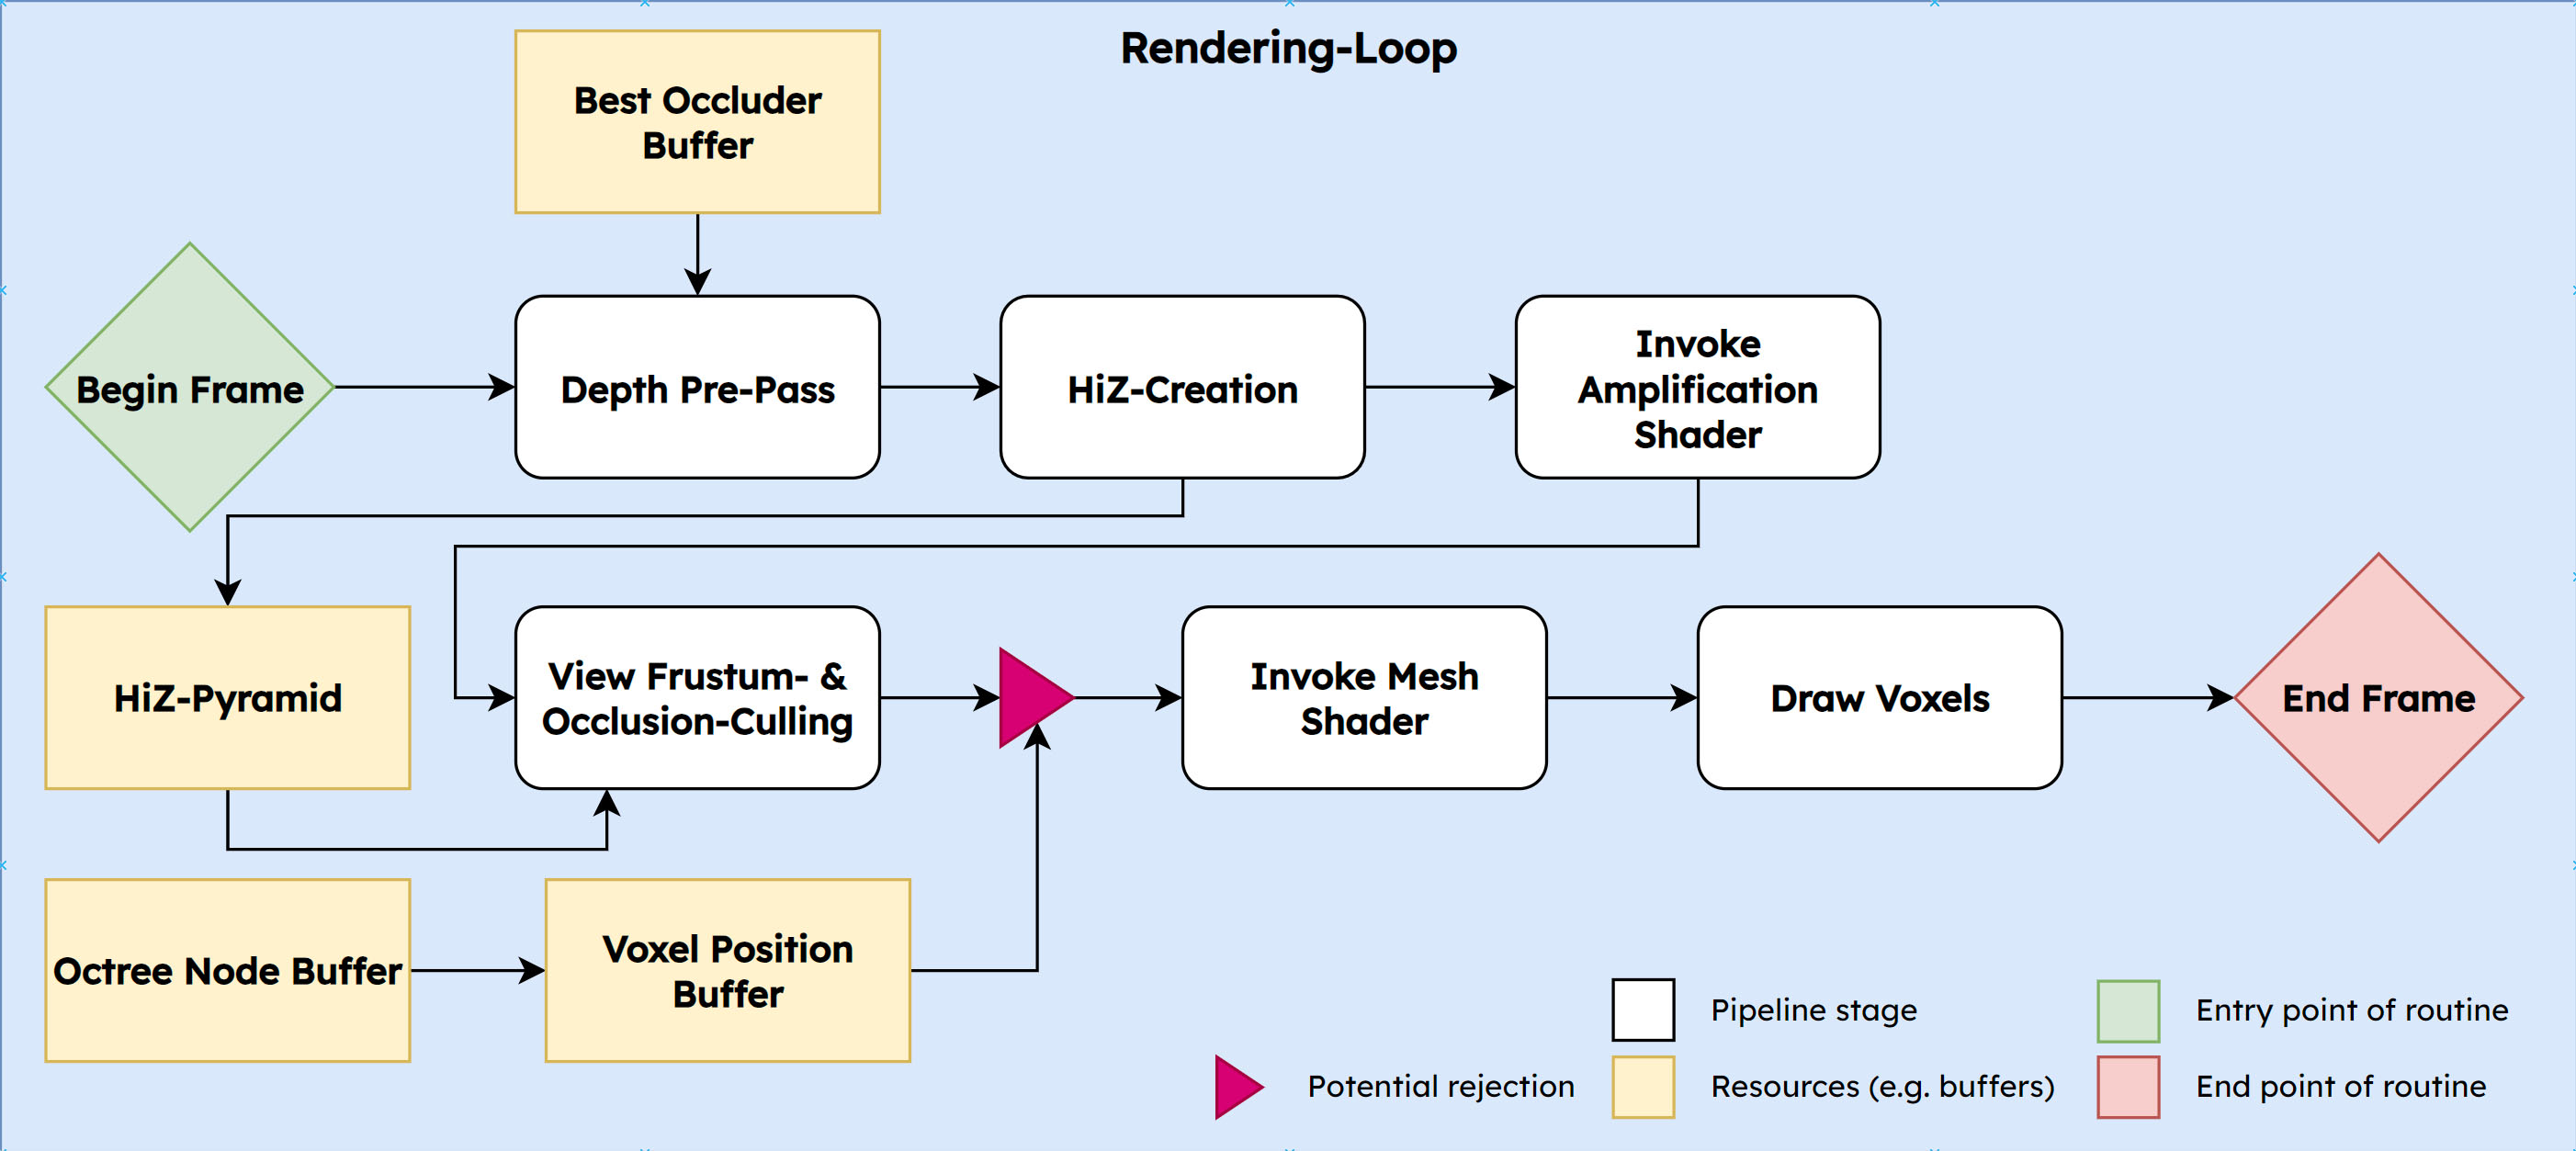
\includegraphics[width=\linewidth]{images/graphics/rendering-loop.jpg}
    \caption{The rendering loop of the rendering pipeline. The red sub-stage of the render loop marks the dispatch 
    of the meshlets, involving the voxel positions and the octree node data. If an octree node or voxel is considered 
    to be culled, the loop ends with the task shader.}
    \label{fig:pipeline-loop}
\end{figure}

\noindent
The rendering loop consists of three main steps: The depth pre-pass including \ac{HiZ} generation, the 
task shader, and the mesh shader. The different stages consume and generate various data buffers 
and textures, as shown in Figure \ref{fig:pipeline-loop}. 

\subsection*{Depth Pre-Pass} \label{subsec-depth-prepass}

The frame computation starts by computing the depth pre-pass, which is the custom render pass central 
to the occlusion culling. In this pass, a compute shader is invoked that takes the best occluders and 
draws them to the depth buffer. This depth pass does not draw to the back buffer, making the computation 
relatively efficient. To get a better understanding of what this means, Figure \ref{fig:best-occluder-viz} 
shows the best occluders. Note that the best occluders in this visualization are not hierarchically 
aggregated, which results in a slightly different visual result than what the actual depth buffer shows. 

\begin{figure}[h]
    \centering
    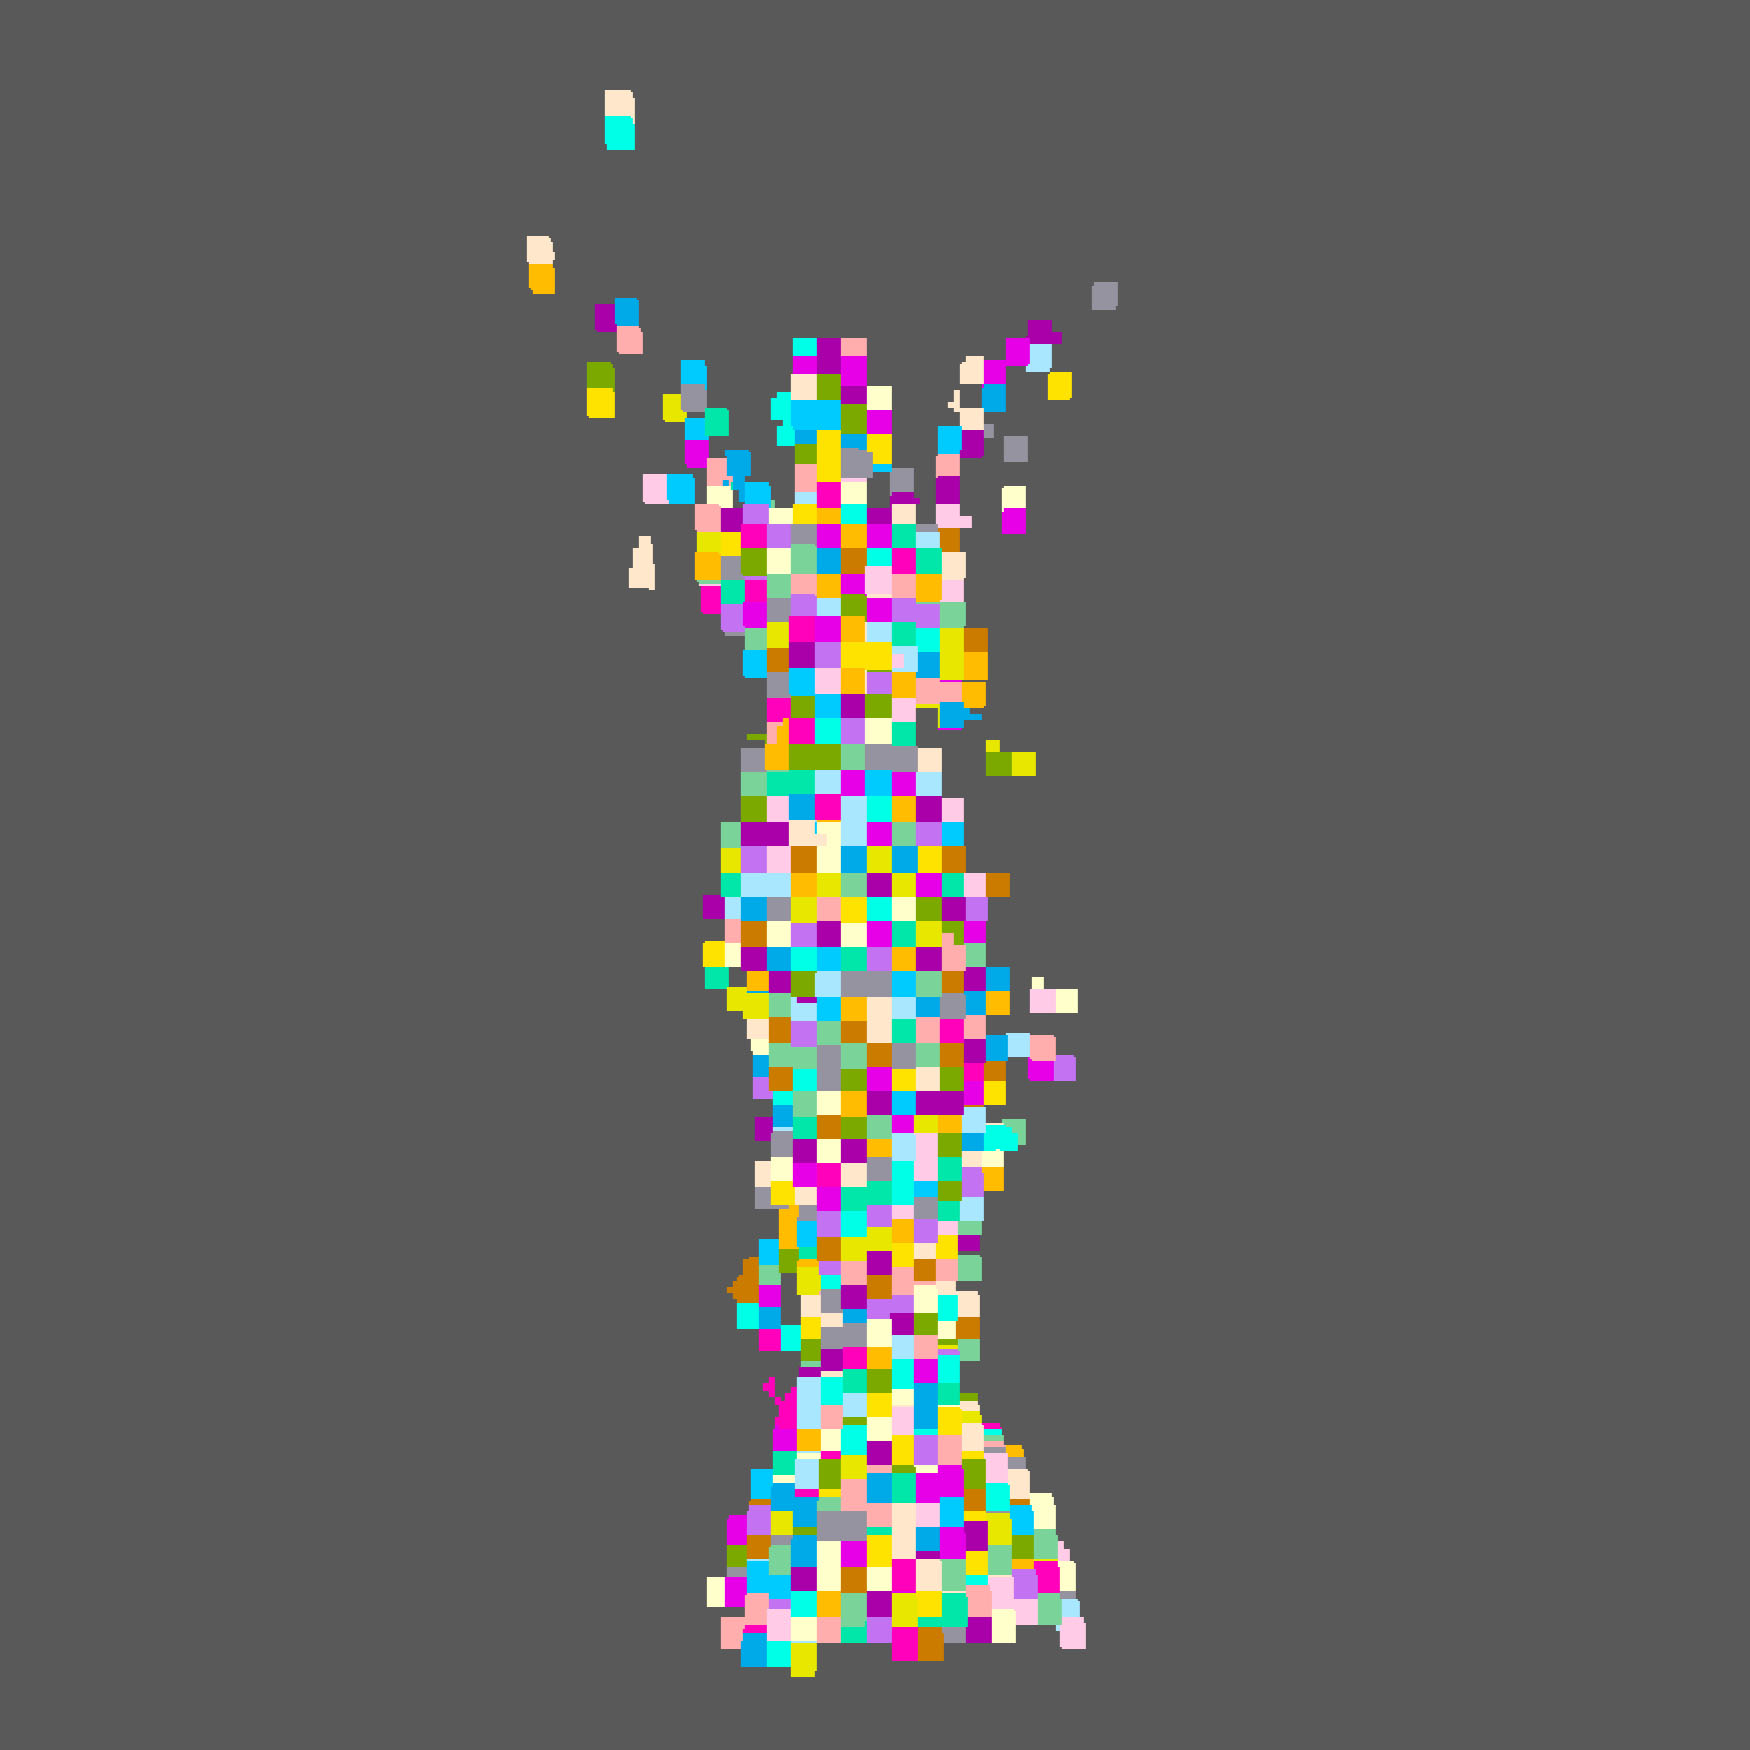
\includegraphics[width=200px]{images/graphics/lucy-best-occluders-viz.jpg}
    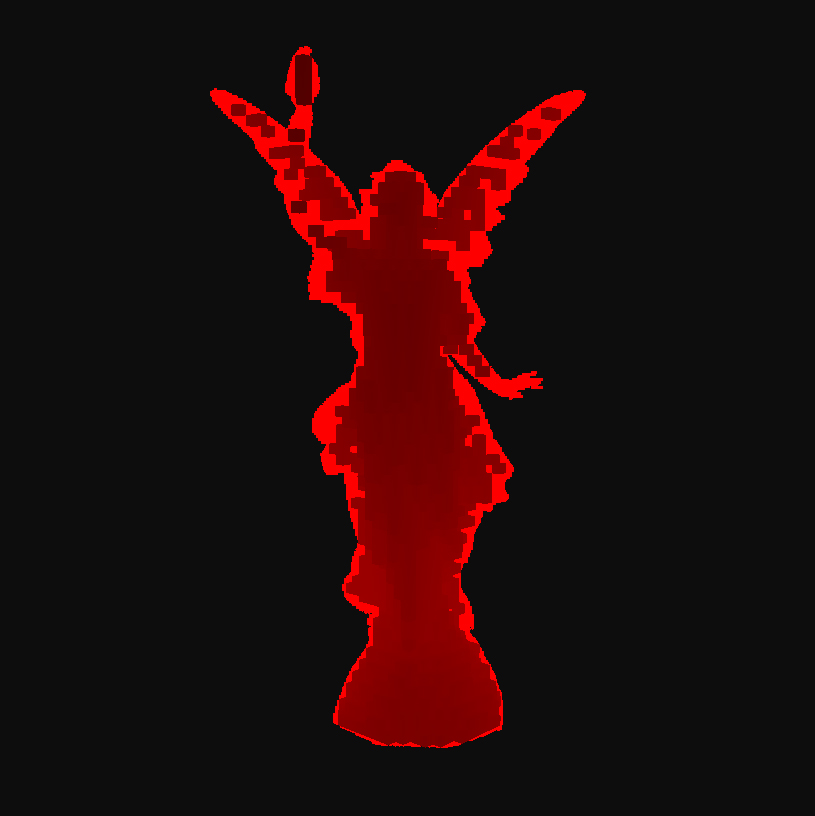
\includegraphics[width=200px]{images/graphics/lucy-best-occluders-diff-viz.jpg}
    \caption{A visualization of the best occluders (left) and the best occluders blended with a silhouette 
    of the whole voxel model (right). Each color represents one octree node which is considered to be a best occluder.
    The best occluders describe the non-visible core of the model and can be aggregated and used to occlude 
    many non-visible voxels during rendering.}
    \label{fig:best-occluder-viz}
\end{figure}


\subsection*{HiZ Generation} \label{subsec-highz-generation}

[@TODO: here is a jump from mip lvl 1 to full z-pyramid!]
After drawing the best occluders to the depth buffer, it is copied into the \ac{HiZ} texture resource. Subsequently, 
the z-pyramid is generated by a compute shader, which samples four texels of the input texture (the full resolution 
depth buffer) and outupts the lowest z-value to the respective higher mip level. After all mip levels are constructed, 
the \ac{HiZ}-pyramid can be used for occlusion culling. The final \ac{HiZ}-pyramid is illustrated in figure 
\ref{fig:lucy-hiz-pyramid}. In the pipeline diagram in Figure \ref{fig:pipeline-loop}, this chain of mip-maps is shown 
as the \ac{HiZ}-pyramid.

\begin{figure}[h]
    \centering
    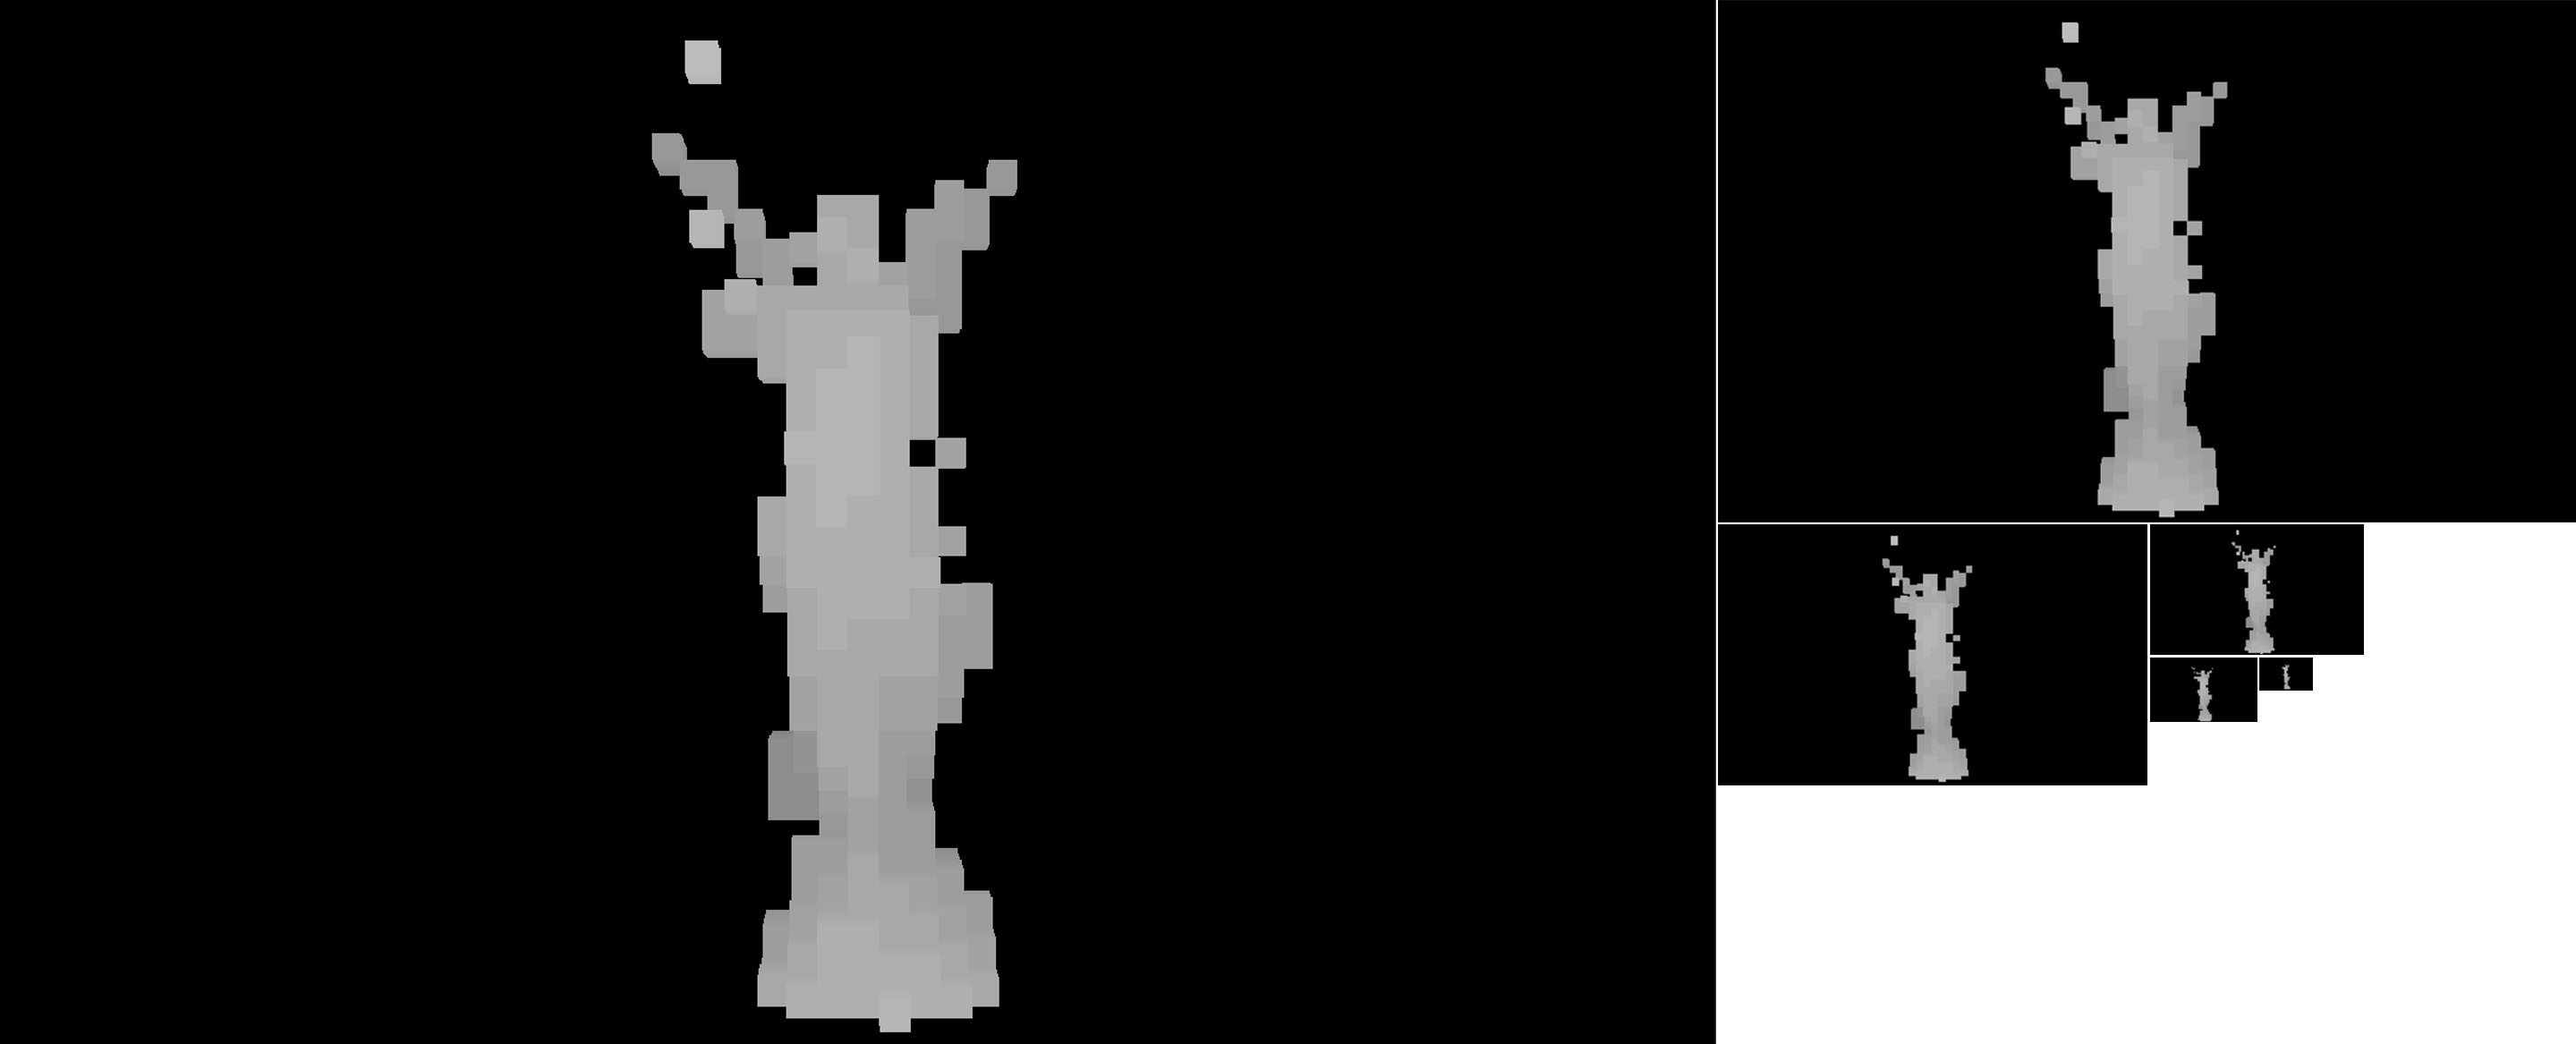
\includegraphics[width=\linewidth]{images/graphics/lucy-hiz-pyramid-inverted.jpg}
    \caption{The \ac{HiZ}-pyramid featuring the full resolution depth buffer as well as the individual mip map 
    levels. The color representation was inverted for better visualization.}
    \label{fig:lucy-hiz-pyramid}
\end{figure}


\subsection*{Culling} \label{subsec-task-shader}

Now, the task shader is invoked, each threadgroup operating on one octree node. It decides which 
meshlets are drawn. This implementation uses view frustum culling to cull octree nodes, which are 
not visible. Figure \ref{fig:lucy-frustum-culling} shows a partially culled model from a different 
perspective. 

[@TODO: Change model to stanford bunny!]
\begin{figure}[h]
    \centering
    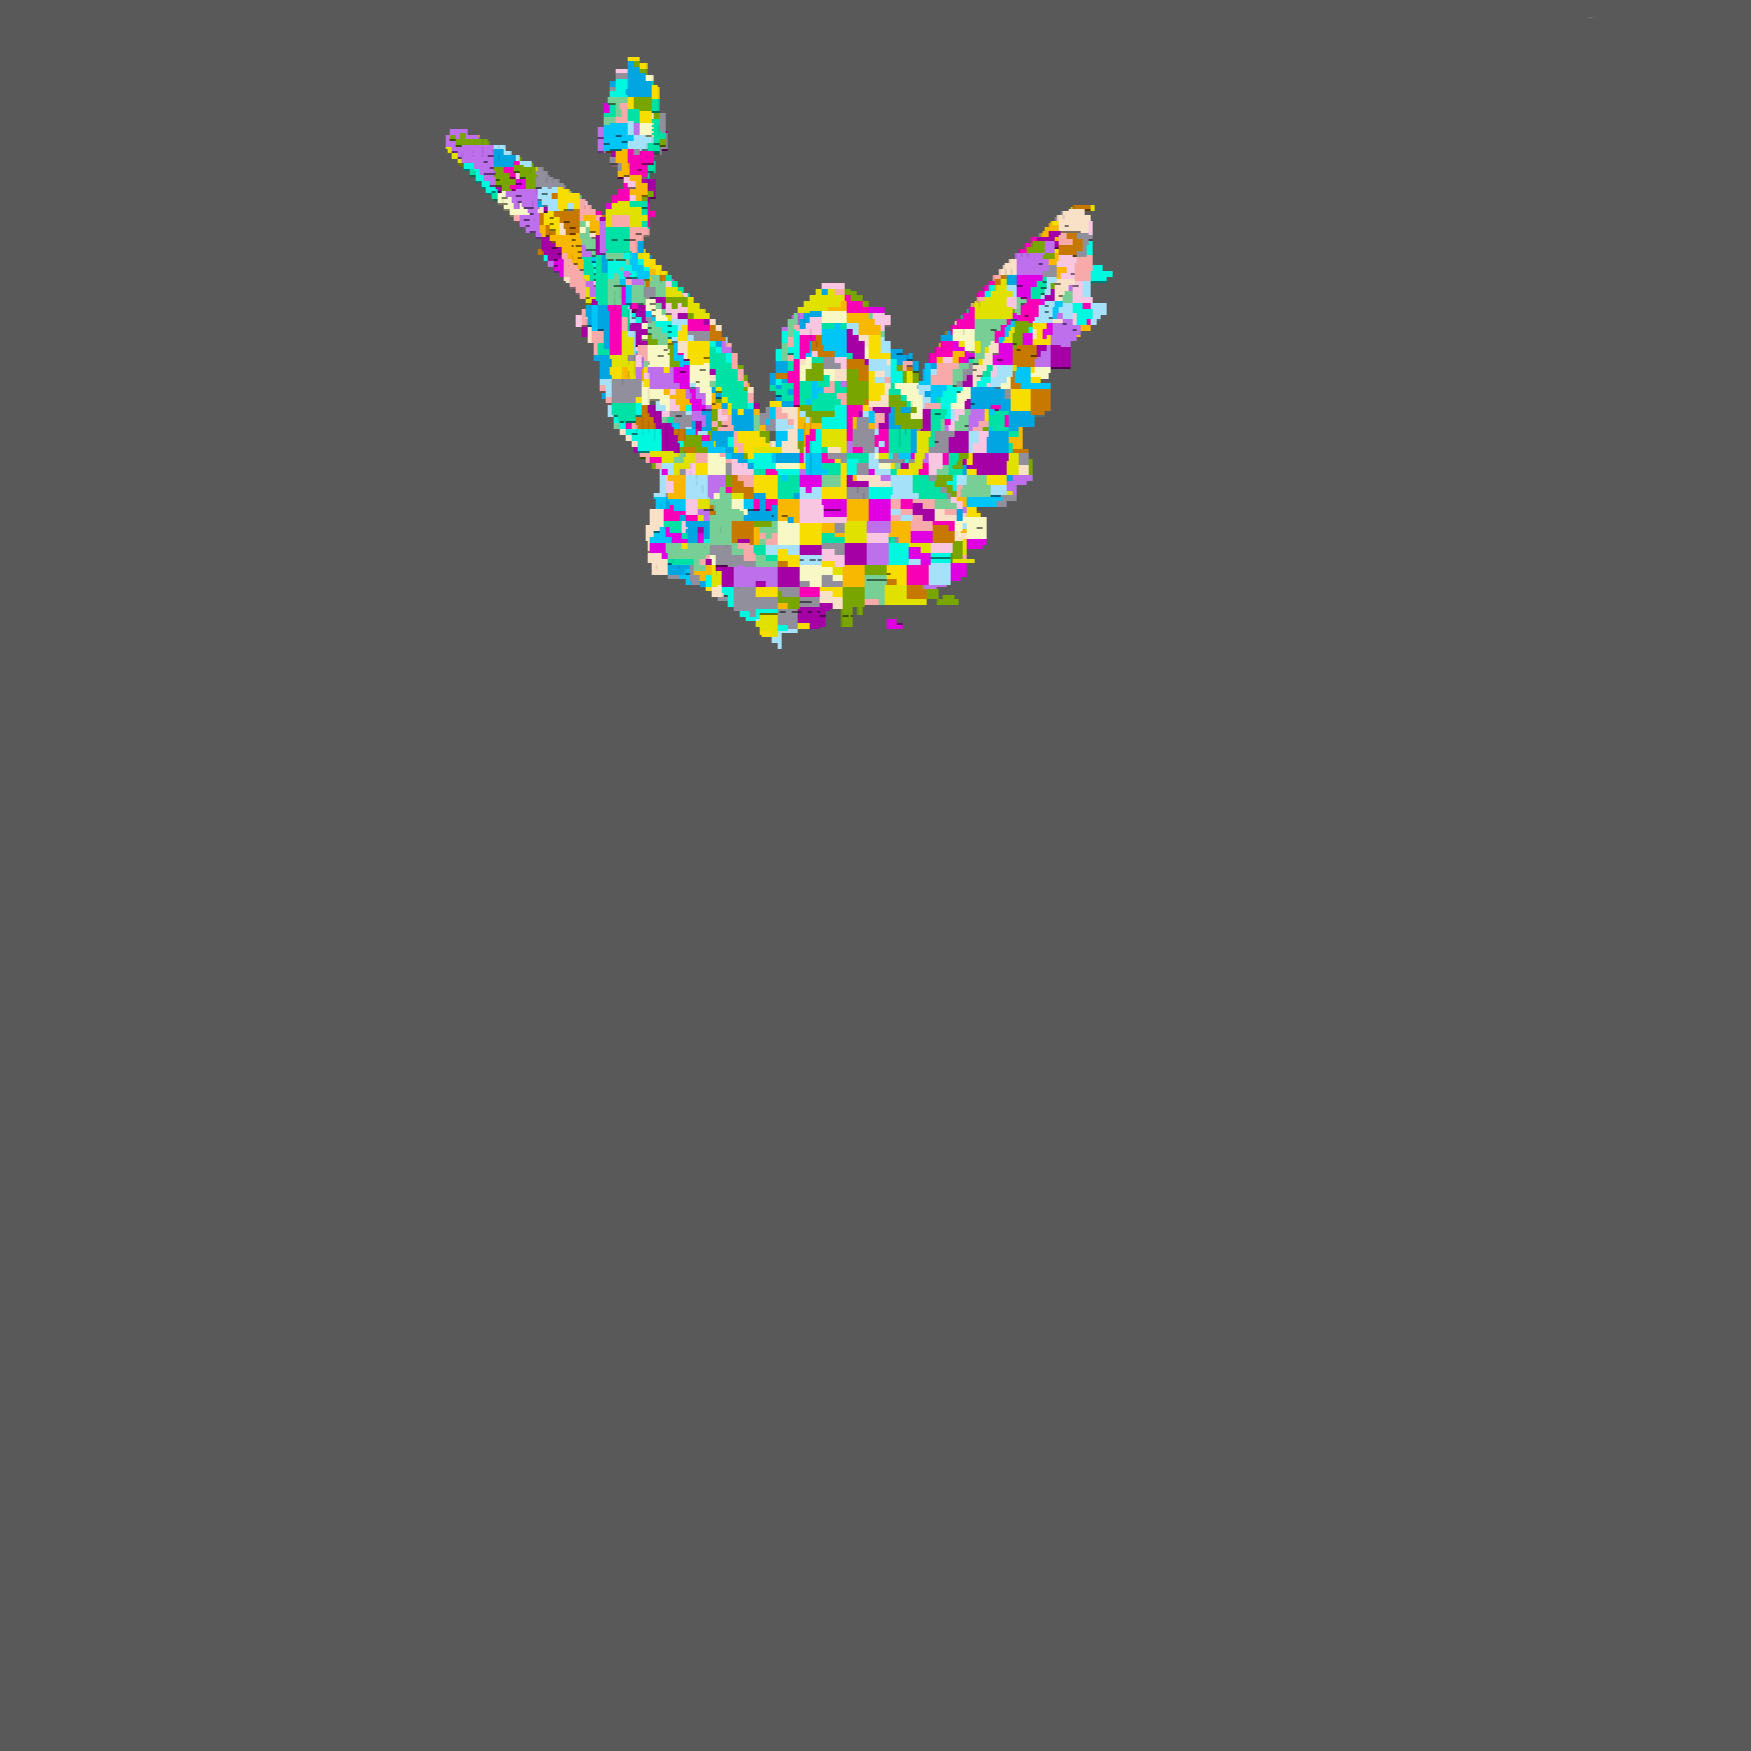
\includegraphics[width=200px]{images/graphics/lucy-frustum-culling.jpg}
    \caption{The whole \emph{Lucy} model culled against the view frustum. Octree nodes which are not in the 
    view frustum are being culled and are therefore not visible.}
    \label{fig:lucy-frustum-culling}
\end{figure}

\noindent [@TODO: Check if meshlets or octree nodes are culled in the end]
Nodes that were not culled using the view frustum are then drawn, checking each voxel for occlusion against the 
\ac{HiZ}-texture and its mip maps. This operation introduces additional overhead, which is normal for any acceleration structure. 
The goal is always to apply it to a scenario where the additional overhead is compensated by the acceleration it provides. 
In this case, the visible voxels might have to pass the whole \ac{HiZ} structure. The non-visible voxels, however, will likely 
exit early after just a few operations, comparing against the mip map hierarchy. In a volumetric representation, the candidates 
for non-visible voxels are plenty, as usually, only a fraction of the voxel data needs to be drawn at any time. Essentially, 
all voxels but the outer, visible layer can be omitted. \\

\noindent
The voxels that passed all tests are finally dispatched for the final draw call, keeping the memory bandwidth to a minimum 
since the geometry, UVs, normals, and more can easily be determined from the position alone and thus created on-chip. \\


\subsection*{Drawing} \label{subsec-mesh-shader}

The mesh shader executes the appropriate transformations, constructs a uniform voxel around the voxel position, 
and outputs the geometry. The voxels in a \ac{GPU}-driven approach can be completely generated on the \ac{GPU}, 
minimizing the memory bandwidth used per frame. This optimization technique is not only efficient but also 
trivial for uniform, static voxel geometry. When dispatching one voxel per thread, one voxel corresponds 
to one meshlet, making pre-computation completely redundant, as opposed to the common precomputation of meshlets, 
as mentioned in Chapter \ref{sec-mesh-shading}.


\section{Occlusion Culling Algorithm} \label{sec-occlusion}

The occlusion culling algorithm is the central part of the pipeline and thus deserves a more detailed coverage. The 
basic implementation is very similar to the ones provided by Aaltonen et al., Greene et al., or Karis et al. 
\cite{Aaltonen2015,Greene93,Karis2021}. It relies on the pre-computations discussed above and can be applied to the 
octree nodes or to individual meshlets. Usually, octree nodes are culled in this process, as \cite{AkenineMoeller2018}
points out. However, using the mesh shading pipeline, it has become possible to cull more fine granular by using 
meshlet bounding volumes as occludees. One advantage is that geometry can be culled, even when the occluder doesn't 
fully overlap the octree node. Therefore, even small instances in the scene can occlude a lot of geometry, resulting 
in better performance overall. On the other hand, this approach requires a lot more computations because all meshlets 
are checked against the \ac{HiZ}-pyramid. Eventually, it is necessary to make precise measurements in order to find out 
which approach works best under the given circumstances. In general, it is hard to predict the performance of 
parallelized \ac{GPU} computations. In Chapter \ref{cpt-experiment}, the culling of octree nodes is compared against the 
culling of individual.


\subsection*{Visibility Computation} \label{subsec-visibility-computation}

As mentioned before, the task shader is used to pre-select and pre-process the scheduled geometry data, 
which in this case is just the position of an individual octree node and all the voxels inside of the node. 
This precomputational step is used for visibility checking, i.e., view frustum culling and occlusion culling. 
Since the task shader is just a general term for any compute shader used before dispatching the meshes, 
this pipeline step is realized using the standard compute architecture. \\

\noindent   [@TODO: write min z and max z in mathematical format]
To check for visibility, \emph{projected bounding boxes} need to be constructed and checked against the 
\ac{HiZ}-pyramid. This step can be highly parallelized by using one \ac{GPU} thread per bounding box 
calculation. The first step involves the projection of the bounding box onto the view plane, which results 
in a clip-space representation of the data. This early projection is done for all eight vertices of the 
bouding box, so the minimum and maximum values on each axis can be calculated to end up with clip space 
and eventually with screen space coordinates. The min and max values for each axis represent a screen 
space rectangle, which can be used for the depth test. The rectangle has the following characteristics:

\begin{itemize}
    \item the minimum and maximum \emph{x} and \emph{y} values describe the four corners of the rectangle and
    \item the minimum \emph{z} value describes the \emph{depth} of the rectangle, i.e. nearest vertex of the bounding box.
\end{itemize}

\noindent
The rectangle can be transformed into screen space and can be expressed as UV coordinates for sampling the 
\ac{HiZ}-pyramid. To check for visibility, all corners of the rectangle are assumed to be at the same distance 
from the camera, i.e., to have the same depth value. This depth value is the minimum \emph{z} value calculated earlier.
This way, as long as any corner of the rectangle is located \emph{in front} of the best occluders stored in the 
\ac{HiZ}-pyramid, the rectangle could be visible partially or completely. Conversely, as long as all corners of 
the rectangle are located behind the best occluder, the rectangle must be completely occluded. A visualization of 
this process is shown in Figure \ref{fig:screen-space-occlusion-test}.

\begin{figure}[h]
    \centering
    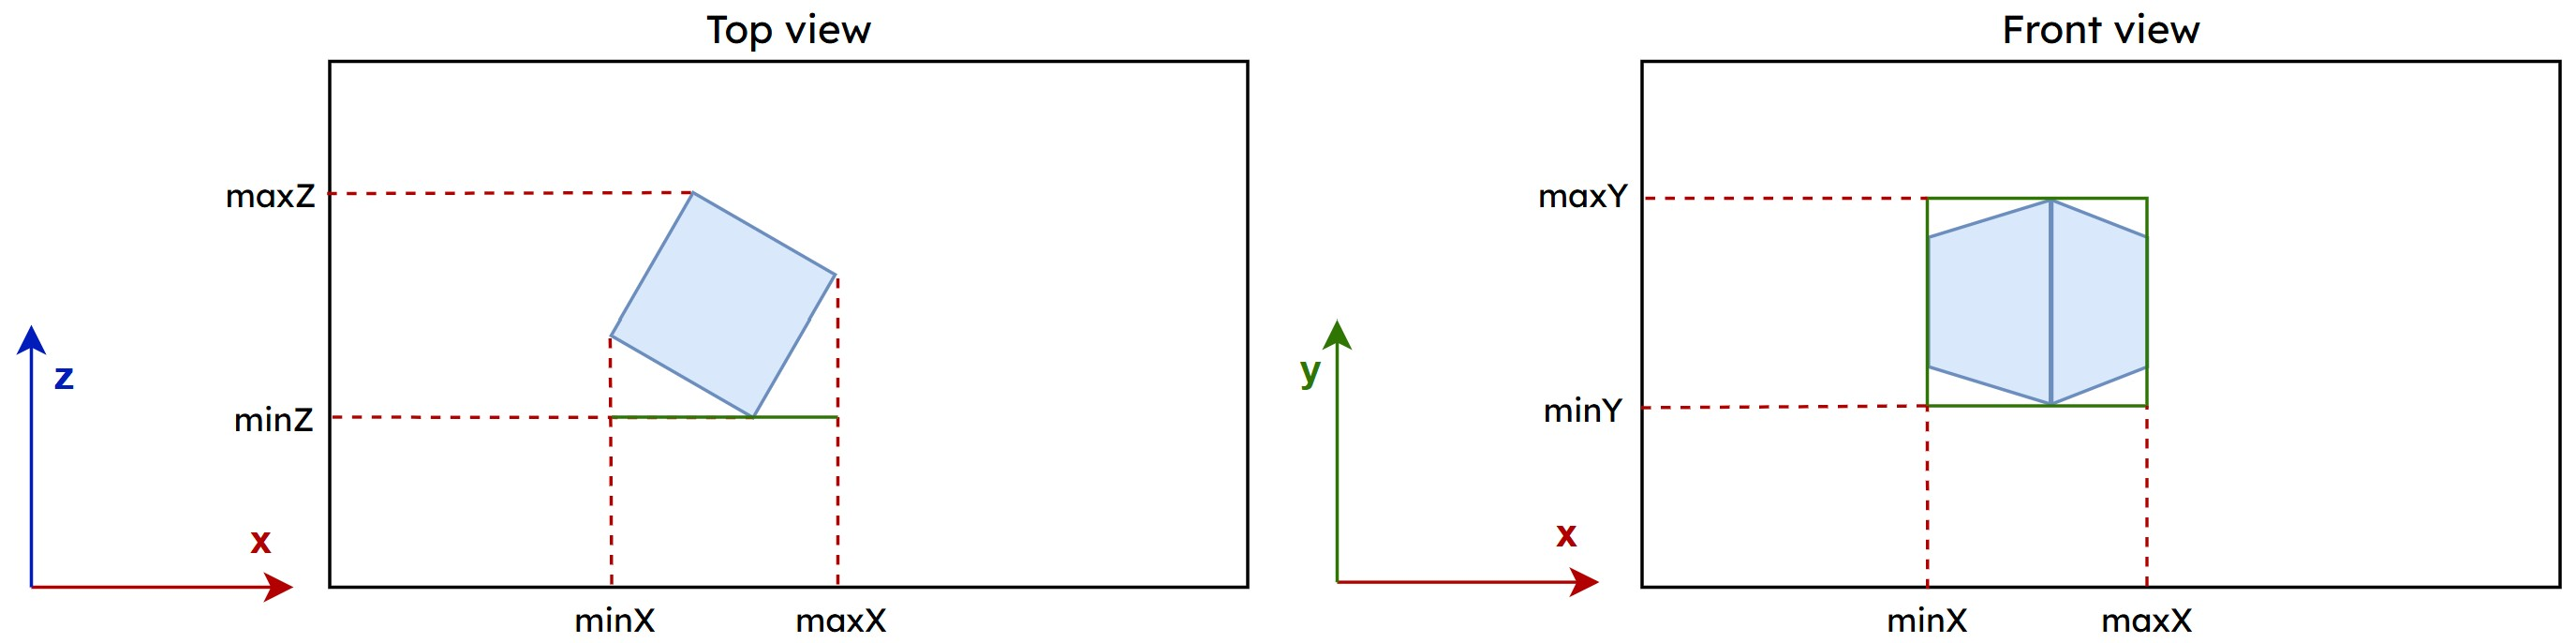
\includegraphics[width=\linewidth]{images/graphics/screen_space_occlusion_test.jpg}
    \caption{The occlusion test is done in screen space using the minimum and maximum boundaries. The octree node 
    is shown in blue, and the respective minimum and maximum values are traced by the dotted red lines. The green 
    line represents the rectangle as viewed from above (left). The same rectangle is shown from a front view as a 
    representation of the octree nodes screen space occupancy (right).}
    \label{fig:screen-space-occlusion-test}
\end{figure}

\noindent
Now the hierarchy is traversed until the node is found to be fully occluded or until the hierarchy is fully traversed 
and the node is found to be visible. Note that the area that is checked is not perfectly congruent with the actual 
projected boundary box. This can lead to edge cases, where a few octree nodes are drawn, although they are actually 
completely occluded. Still, this algorithm is completely conservative, meaning that it does not occlude any geometry 
that should in fact be visible.

\begin{figure}[h]
    \centering
    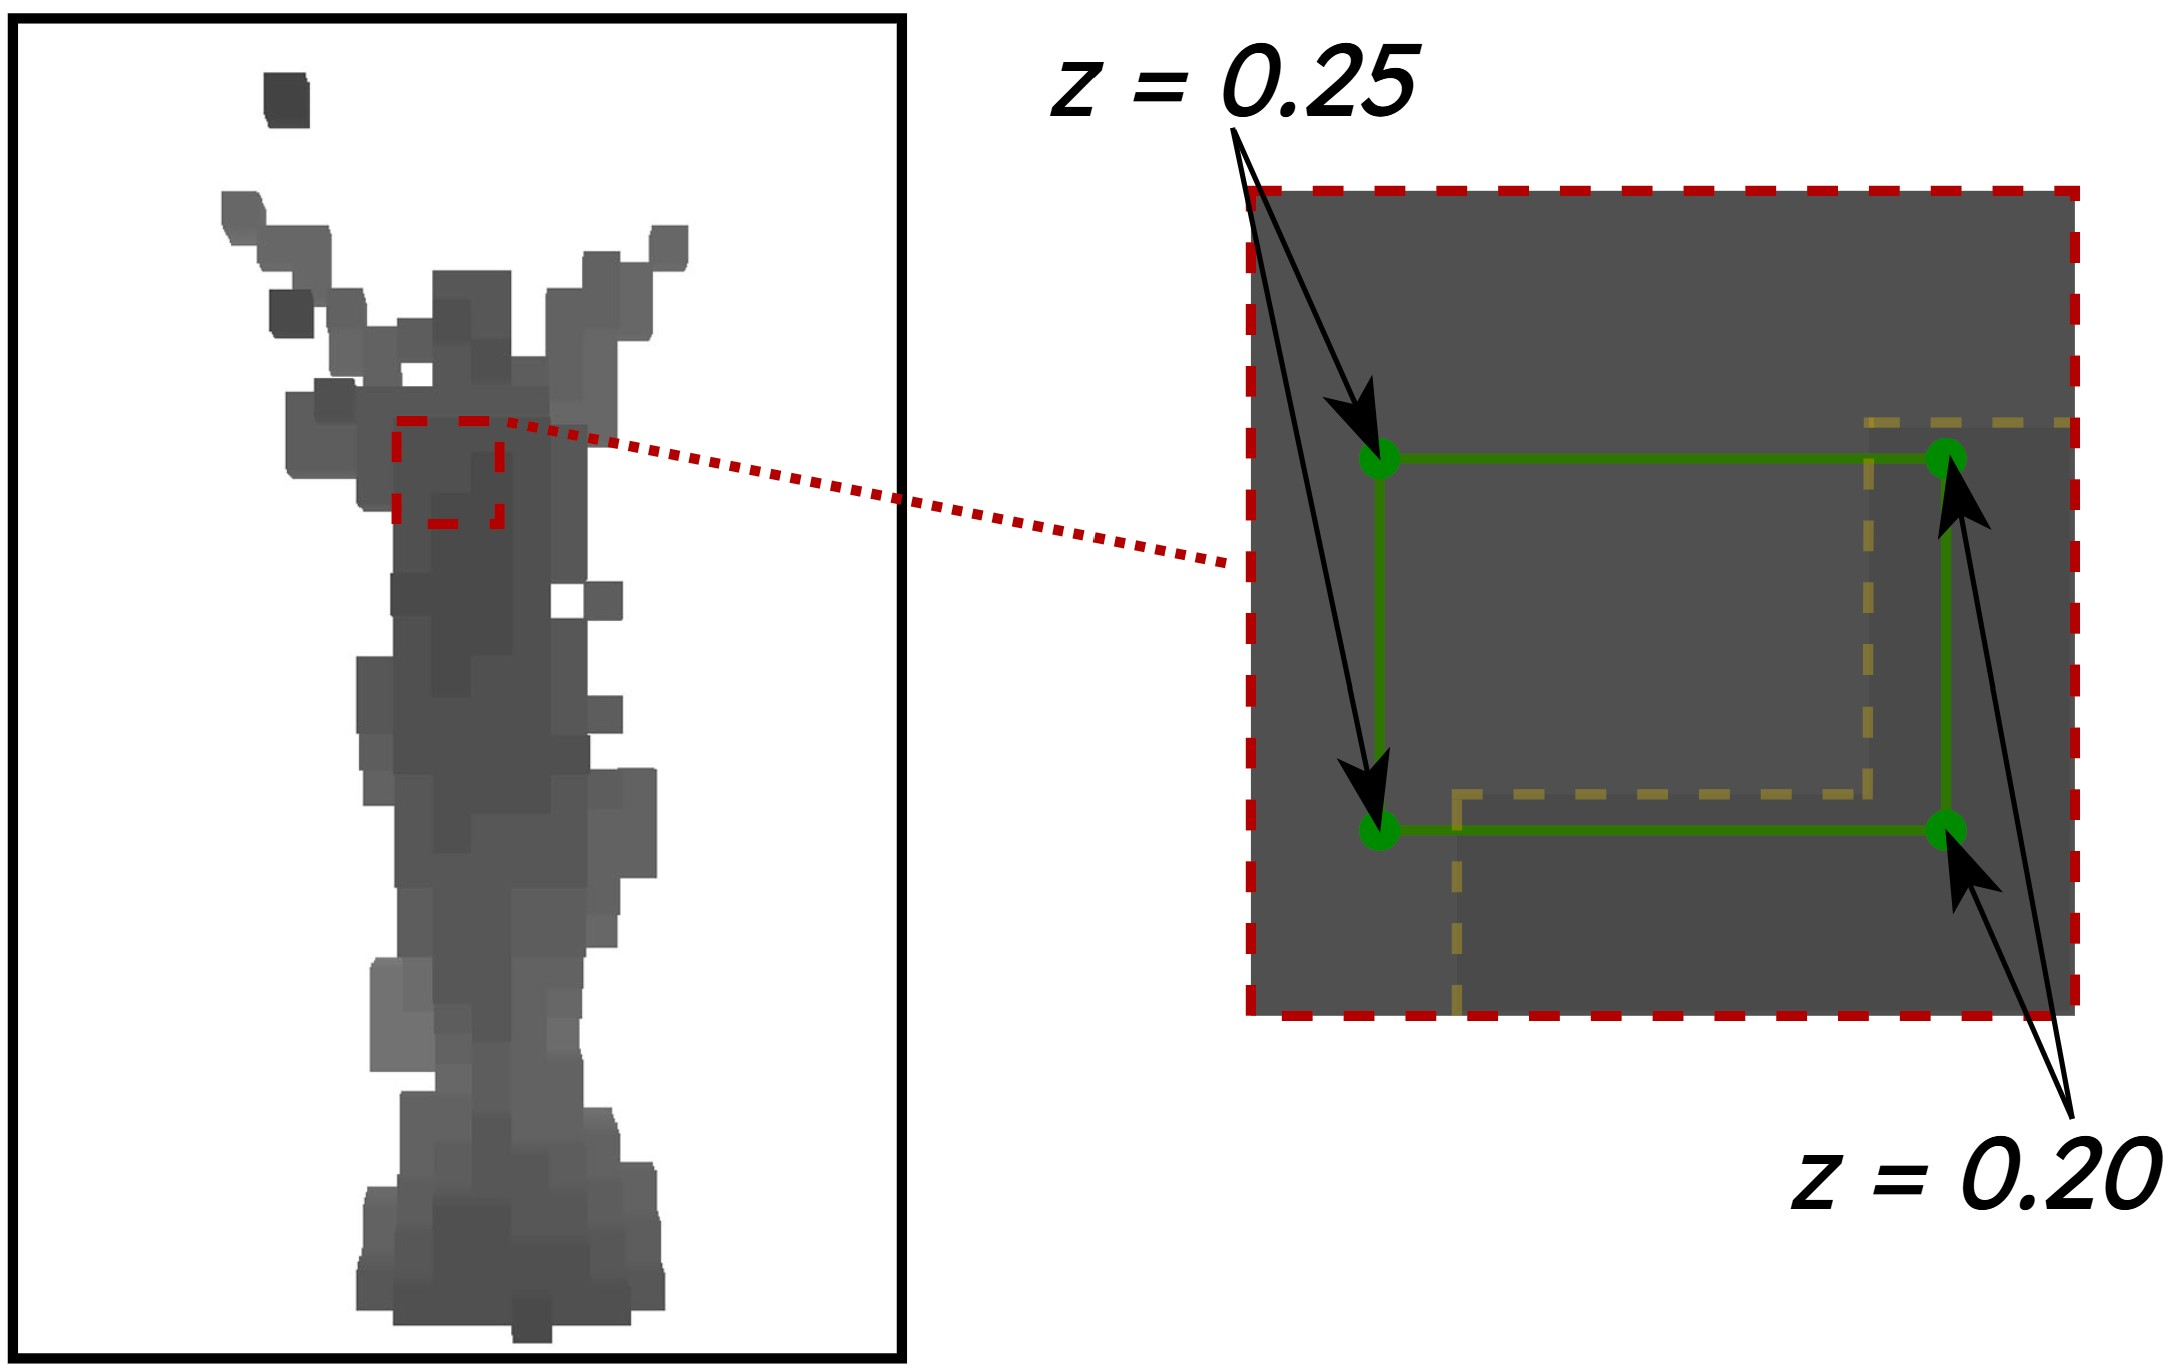
\includegraphics[width=\linewidth]{images/graphics/visibility-hiz-sampling.jpg}
    \caption{The \ac{HiZ}-pyramid being sampled using the corners of the screen-space rectangle, shown in green. 
    The dotted yellow line resembles the border between different depth values in the buffer. Sampling the four 
    corners can provide up to four different depth values. The smallest one being the "nearest" occluder.}
    \label{fig:visibility-hiz-sampling}
\end{figure}


\noindent
The complete occlusion culling routine computes the bounding box corners as \emph{UV} coordinates so it is independent 
from the mip level the depth values are checked against. In the best case, the visibility can be determined by using 
the coarsest mip level. In the worst case, all mip levels up to the full resolution depth buffer need to be checked.
The routine is shown in listing \ref{lst-occlusion-culling-algo} as pseudocode.

\fbox{
\begin{minipage}{\linewidth}
\begin{algorithm}[H]
\SetAlgoLined
\KwIn{float4 basePosAndScale}
\KwResult{Boolean indicating whether a bounding box is visible}

\SetKwFunction{FMain}{IsVisible}
\SetKwProg{Fn}{Function}{:}{}
\Fn{\FMain{float4 basePosAndScale, Texture2D HiZPyramid}}
{
    float4 center $\gets$ float4(basePosAndScale.xyz, 1.0f)\;
    float scale $\gets$ abs(basePosAndScale.w)\;
    \BlankLine

    float minX $\gets$ GetMinXFromProjectedBoundingBox(center, scale)\;
    float maxX $\gets$ GetMaxXFromProjectedBoundingBox(center, scale)\;
    float minY $\gets$ GetMinYFromProjectedBoundingBox(center, scale)\;
    float maxY $\gets$ GetMaxYFromProjectedBoundingBox(center, scale)\;
    float minZ $\gets$ GetMinZFromProjectedBoundingBox(center, scale)\;
    \BlankLine

    Rect uvRect $\gets$ CalculateUVRect(minX, maxX, minY, maxY, minZ)\;
    \BlankLine

    \For{$mipLevel \gets HiZPyramid.GetNumMipLevels() - 1$ \KwTo $0$}{
        float depthVertex1 $\gets$ HiZPyramid.Sample(uvRect.vertex1, mipLevel)\;
        float depthVertex2 $\gets$ HiZPyramid.Sample(uvRect.vertex2, mipLevel)\;
        float depthVertex3 $\gets$ HiZPyramid.Sample(uvRect.vertex3, mipLevel)\;
        float depthVertex4 $\gets$ HiZPyramid.Sample(uvRect.vertex4, mipLevel)\;
        \BlankLine

        \If{max(depthVertex1, depthVertex2, depthVertex3, depthVertex4) < minZ}{
            \Return{false}\;
        }
    }

    \Return{true}\;
}
\caption{Occlusion Culling algorithm.}
\label{lst-occlusion-culling-algo}
\end{algorithm}
\end{minipage}
}
    
\vspace{0.5cm}


\section{Implementation Limitations}

- thread dispatch limited to 65536


[@TODO: Mention view frustum culling in depth pre pass]
[@TODO: Mention that experiment was limited by directly using the highest resolution z buffer in cpt experiment!]


    \chapter{Experiment} \label{cpt-experiment}

When considering occlusion culling algorithms that can be used in a given use case, the runtime 
performance is a critical aspect. But runtime performance is a multi-dimensional measure, in that 
most algorithms provide results under specific circumstances and by setting several constraints.
To be able to evaluate the strengths and weaknesses of the given implementation, an in-depth  
experiment was conducted and evaluated, highlighting a diverse set of measured data. \\ 

\noindent
The method of profiling performance was chosen because it allows for an in-depth analysis of the 
pipeline steps. When accurately measuring the two configurations, per-meshlet culling and 
per-octree culling, the difference between both can be evaluated by looking at various pipeline 
steps and their timings. A cross-comparison between pipelines using different models can additionally 
provide insights into why the computation times scale and how the complexity of the scene refers to 
the scaling.\\

\noindent
Ultimately, the two approaches \emph{per-octree node occlusion culling} and \emph{per-meshlet occlusion culling} 
were compared in this experiment, both in terms of how many voxels could be culled and in terms of the respective 
overhead and the performance gains. \\

\noindent
First, the experiment is evaluated in how it shows the differences between the pipelines. In this context, various 
factors are discussed and it is presented how these factors were taken into account during the experiment. AAfter 
that, the tools that were used to perform the measurements are presented, as well as the models, which were tested.
Finally, the results are discussed by presenting the measurements for each model. A brief summary of the results is 
given in the end, aggregating average data from all the tests performed during the experiment.

\section{Experimental Evaluation} \label{sec-experimental-evaluation}

To evaluate the key differences and the runtime performance in general, several aspects had to be considered.
Unfortunatly, comparing the occlusion culling implementation to an alternative implementation was not within the 
scope of this work, so efforts were made in order to evaluate the pipeline and its performance from a conceptual 
point of view and compared to the plain pipeline, without any occlusion culling at all. This includes two different 
versions of occlusion culling, one based on culling octree node as it can be implemented without the use of the 
Mesh Shading pipeline. The other one is based on per-meshlet occlusion culling, which makes use of the more parallel 
computation capabilities of the \ac{GPU}. \\

\noindent
This sections highlights the major aspects which were considered for the experiment and were evaluated during the 
test runs. All aspects aim to demonstrate how the occlusion culling affected the given test scene and how the 
computations differ compared to the plain pipeline. Later, use cases are considered which can be compared to 
alternative algorithms on a high level. However, keep in mind that it is up to future measurements to quantitavely 
compare the pipeline to alternative approaches. 


\subsection*{Scene Layout} \label{subsec-scene-layout}

Every occlusion culling algorithm somehow relies on spatial information, be it in world space or sceen space. 
Consequently, the scene layout and how the scene changes relative to the camera were important aspects to consider. 
For this experimental setup, a moving camera was used in order to test the ability of the occlusion culling 
algorithm to adapt to different angles of the scene. \\

\noindent
The data was sampled over time using a standardized camera animation, which was following a circular orbit 
around the model, visualized in figure \ref{fig:test-anim-camera-path}. A vertical offset was added to the orbit, 
so the model could be drawn from various angles. This was especially important for models like the \emph{Torus}, 
which are likely to behave very differently when viewed from above compared to when viewed from the side.

\begin{figure}[h]
    \centering
    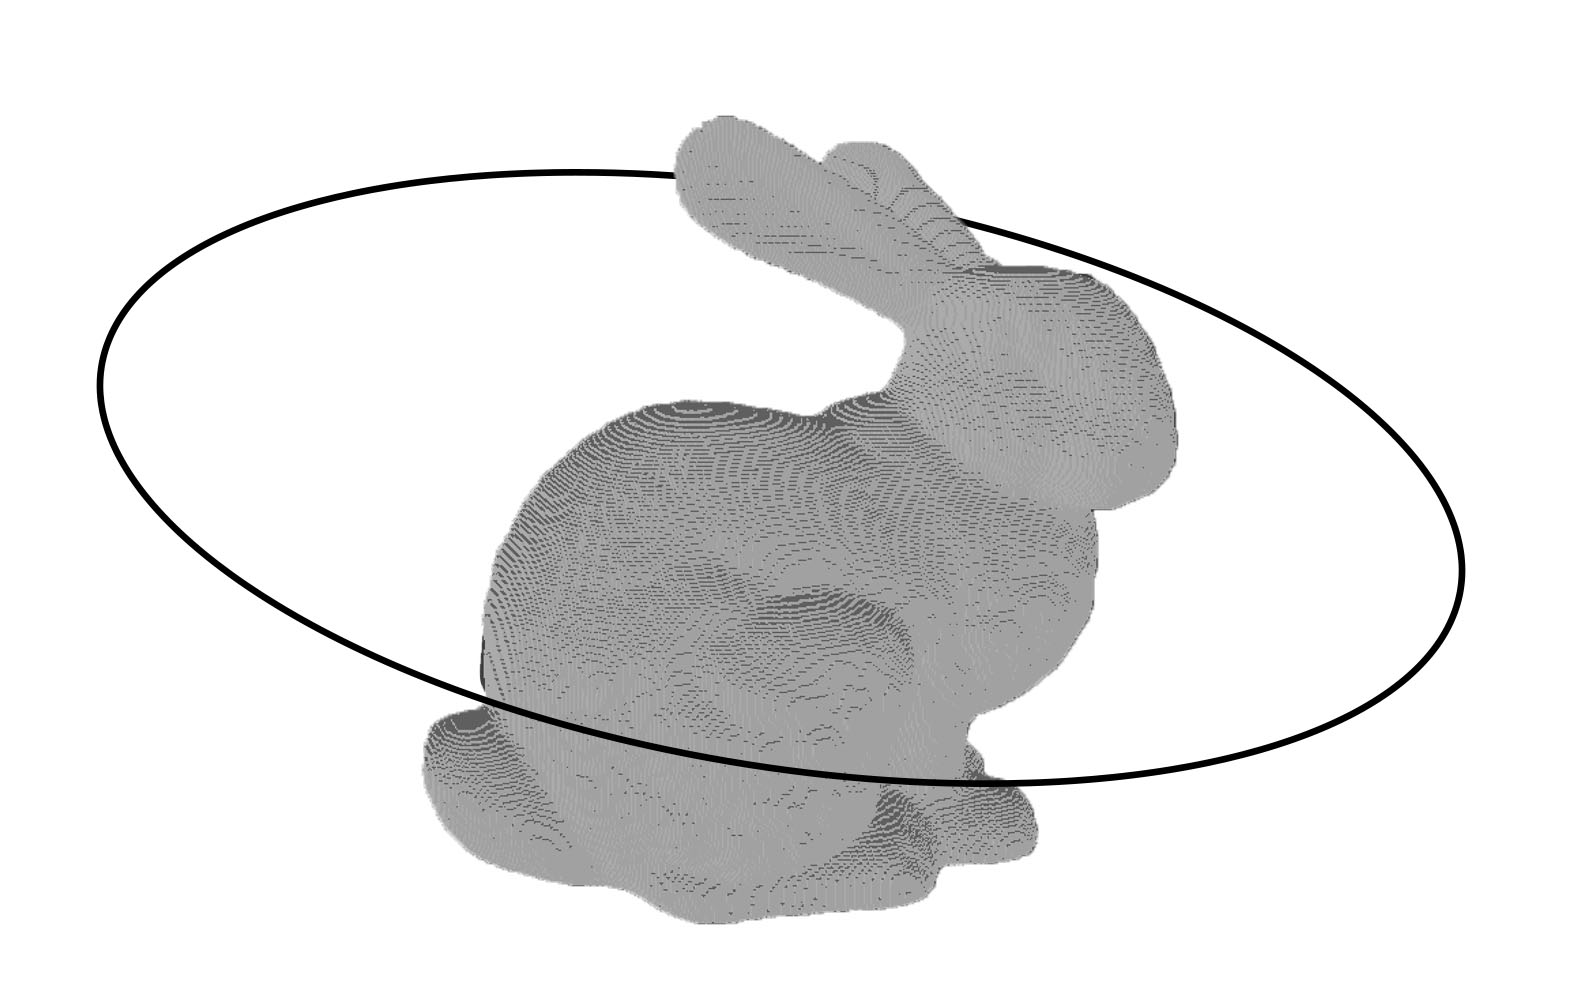
\includegraphics[width=200px]{images/graphics/test-anim-camera-path.jpg}
    \caption{During profiling, the camera is moved along an orbit around the voxel mesh, while being offset to compensate 
    for models, which behave differently when viewed from an angle. The visualization is not to scale, the models 
    are always completely visible and not culled by view frustum culling.}
    \label{fig:test-anim-camera-path}
\end{figure}

\noindent
[@TODO: Consider replacing the last "algorithm" with the actual subelement of the algo (scene data / data dispatch / ...)] 
Another aspect to consider is the model data structure. The voxel models are volumetric representations and thus, 
not hollow. This leaves a large portion of computation to be irrelevant and allows for the occlusion culling to 
optimize the data flow. Different types of models were used to challenge the culling algorithm in different ways. 
In concept, the culling should be optimal on large, dense models with even faces. Consequently, models with 
slopes and holes were tested, to see how best occluders can be computed for diverse geometry. Smaller models might 
also pose a challenge for the optimization, especially when the octree nodes cannot be filled completely. Also, 
different voxel resolutions were used to achieve different amounts of octree nodes in the scene. All these different 
aspects aim to show the strengths and weaknesses of the algorithm and how it can be optimally used in practice. \\

\noindent
The resolution of the voxelization process played a central role in the experimentation process.
For the experiment, the voxel scenes were constrained to be a power of two in length per axis, and a resolution 
of $\emph{256} \times \emph{256} \times \emph{256}$ were used for the performance profiling, resulting in a maximum 
of \emph{16.777.216} voxels. In practice, the maximum amount of voxels was limited by how the data is dispatched 
by the \ac{GPU}. In the implementation, the shader model used (HLSL Shader Model 6.6) was limited to a maximum 
amount of 65.536 threadgroups. That means that the threadgroup size and the amount of constructed octree nodes 
influenced the possible resolutions of the scenes. This limitation can be overcome by scheduling more than one draw 
call, but for this experiment, only one draw call was used. Consequently, the actual maximum amount of voxels in the 
scene was around 3 - 4 million voxels, which was considered enough for this experiment. \\

\noindent
For comparison of particular measures, some of the models were additionally tested using higher or lower resolutions.
Whenever the respective comparison is meaningful, it is highlighted as such.


\subsection*{Timings} \label{subsec-timings}

Ultimately, the time spent for various computations is relevant for the selection of the best algorithm. This is 
a central tool to see how the implementation performs overall in the context of the framework used. The frame 
time is the first measurment to be considered, but not necessarily the most meaningful in a complex pipeline. 
Consequently, the timings for all major pipeline steps were considered, as well as the overall time spend on 
\ac{CPU} and \ac{GPU} computations. 


\subsection*{Visibility and Culling} \label{subsec-visibility-and-culling}

In order to evaluate the general functionality and effectiveness of the pipeline, the voxel model was analysed 
with and without the occlusion culling applied. The amount of culled voxels was compared to the total amount of 
voxels resulting in an overview of how much geometry could be culled for different scene setups. The same is 
valid for the amount of octree nodes. They could also be compared to the amount of best occluders. The more best 
occluders present in a scene, the higher the probability to occlude other voxels or octree nodes. To evaluate 
how much can be optimized during the depth pre pass, the amount of best occluders was compared to the amount 
of voxels representing the best occluders. \\

\noindent
Finally, the actual amount of processed triangles was considered in order to show the actual geometry processed 
by the \ac{GPU}. This data indicates how much work is being scheduled for the vertex transformations, the rasterizer 
and the pixel shader. Ultimately, it decides over the amount of overdraw and should therefore be kept at a minimum.


\subsection*{Additional Overhead} \label{subsec-additional-overhead}

[@TODO: Refresh sentence]
The additional overhead needs to be evaluated compared to the gain in performance by the occlusion culling. 
Because of that, the pipeline is analyzed and the timings are compared to a pipeline without the culling 
algorithm. All per-frame computations are evaluated to see how much resources are spent on culling overhead. 
The results are compared against the acceleration provided by the algorithm.\\

\noindent
To increase the significance of the data, the per-meshlet occlusion culling was compared against the 
per-octree occlusion culling. The difference should be able to show, how the Mesh Shading pipeline 
influences the culling algorithm. The per-meshlet culling was expected to be more precise and to cull 
more voxels, since individual voxels within one octree can be culled, as opposed to per-octree node 
culling, which either renders all voxels within an octree node or culls it completely. 


\subsection*{Measuring Tools} \label{subsec-measuring-tools}

To measure timings and data precisely, a few external tools were used. All tools are part of the industry 
standard and were therefore assumed to be mostly reliable. Still, measuring performance usally comes with 
a minimal overhead which means that the results most likely vary in precision. Also, some of the tools 
provided various ways of coming up with the data. Some data was measured while the profiled application 
was running, and other data was acquired by replaying the command list of the \ac{GPU}. Consequently, all 
measurements referring to one aspect of the application were compared against measurements using the same 
tool and configuration, if not explicitly specified otherwise. \\

\noindent
For the collection of data output, \emph{RenderDoc} \cite{RenderDoc} was used. It is a free, MIT licensed 
rendering debugger, widely used in the industy. For \emph{NVIDIA} specific \ac{GPU} profiling, \emph{NVIDIA NSight} 
\cite{NSight} was used, which is another industry standard profiling and debugging tool. It is only available for 
inspection of \emph{NVIDIA} graphics card computations but provided valuable insights into the rendering pipeline 
and hardware usage. The last tool used is \emph{Microsoft's PIX} \cite{PIX}, which is another performance debugging 
and profiling tool for \emph{Windows} platforms using \emph{Microsoft's DirectX} \ac{API}.


\subsection*{Experimental Environment} \label{subsec-experimental-environment}

[@TODO: Rethink section title]
For the experiment, different hardware setups were used to compare the runtime performance in different environments.
Some more modern hardware was used to profile the best case computations, and older hardware was used for the results 
to different versions of hardware features and capabilities.

\begin{table}[h]          % System setup table
    \begin{tabular}{|lll|}
        \hline
        \multicolumn{3}{|c|}{\textbf{Test setups}}                                                                              \\ \hline
        \multicolumn{1}{|l|}{}                     & \multicolumn{1}{l|}{\textbf{Setup 1}}          & \textbf{Setup 2}          \\ \hline
        \multicolumn{1}{|l|}{\textbf{System Type}} & \multicolumn{1}{l|}{Desktop}                   & Laptop                    \\
        \multicolumn{1}{|l|}{\textbf{CPU}}         & \multicolumn{1}{l|}{AMD Ryzen 9 9950X}         & Intel Ultra 7 155H        \\
        \multicolumn{1}{|l|}{\textbf{Cores}}       & \multicolumn{1}{l|}{16 (32)}                   & 16 (22)                   \\
        \multicolumn{1}{|l|}{\textbf{RAM}}         & \multicolumn{1}{l|}{96 GB}                     & 16 GB                     \\
        \multicolumn{1}{|l|}{\textbf{GPU}}         & \multicolumn{1}{l|}{NVIDIA GeForce RTX 4090}   & Intel Arc Graphics        \\
        \multicolumn{1}{|l|}{\textbf{VRAM}}        & \multicolumn{1}{l|}{24 GB}                     & 128 MB (+ 8972 MB shared) \\
        \multicolumn{1}{|l|}{\textbf{OS}}          & \multicolumn{1}{l|}{Windows 10}                & Windows 11                \\
        \multicolumn{1}{|l|}{\textbf{Model}}       & \multicolumn{1}{l|}{-}                         & ASUS Zenbook 14 (2024)    \\ \hline
    \end{tabular}
    \caption{The experimental setups used to profile the applications performance.}
    \label{tbl:hardware-setup}
\end{table}

\noindent
Note that the use of the Mesh Shading pipeline requires graphics cards that support the pipeline in the first place. 
For \emph{NVIDIA} \ac{GPU}s this is the \emph{Turing} lineup (\emph{NVIDIA RTX 20 series}) and for \emph{AMD} cards 
this would be the \emph{RDNA 2} lineup (\emph{AMD RX 6000 series}). \emph{Intel} \ac{GPU}s support the feature as 
well, starting from their first installment in the dedicated desktop \ac{GPU} series \emph{Intel Arc}. The specs of 
the test setups are listed in table \ref{tbl:hardware-setup}. \\


\subsection*{Models} \label{subsec-models}

\begin{figure}[h]
  \centering
  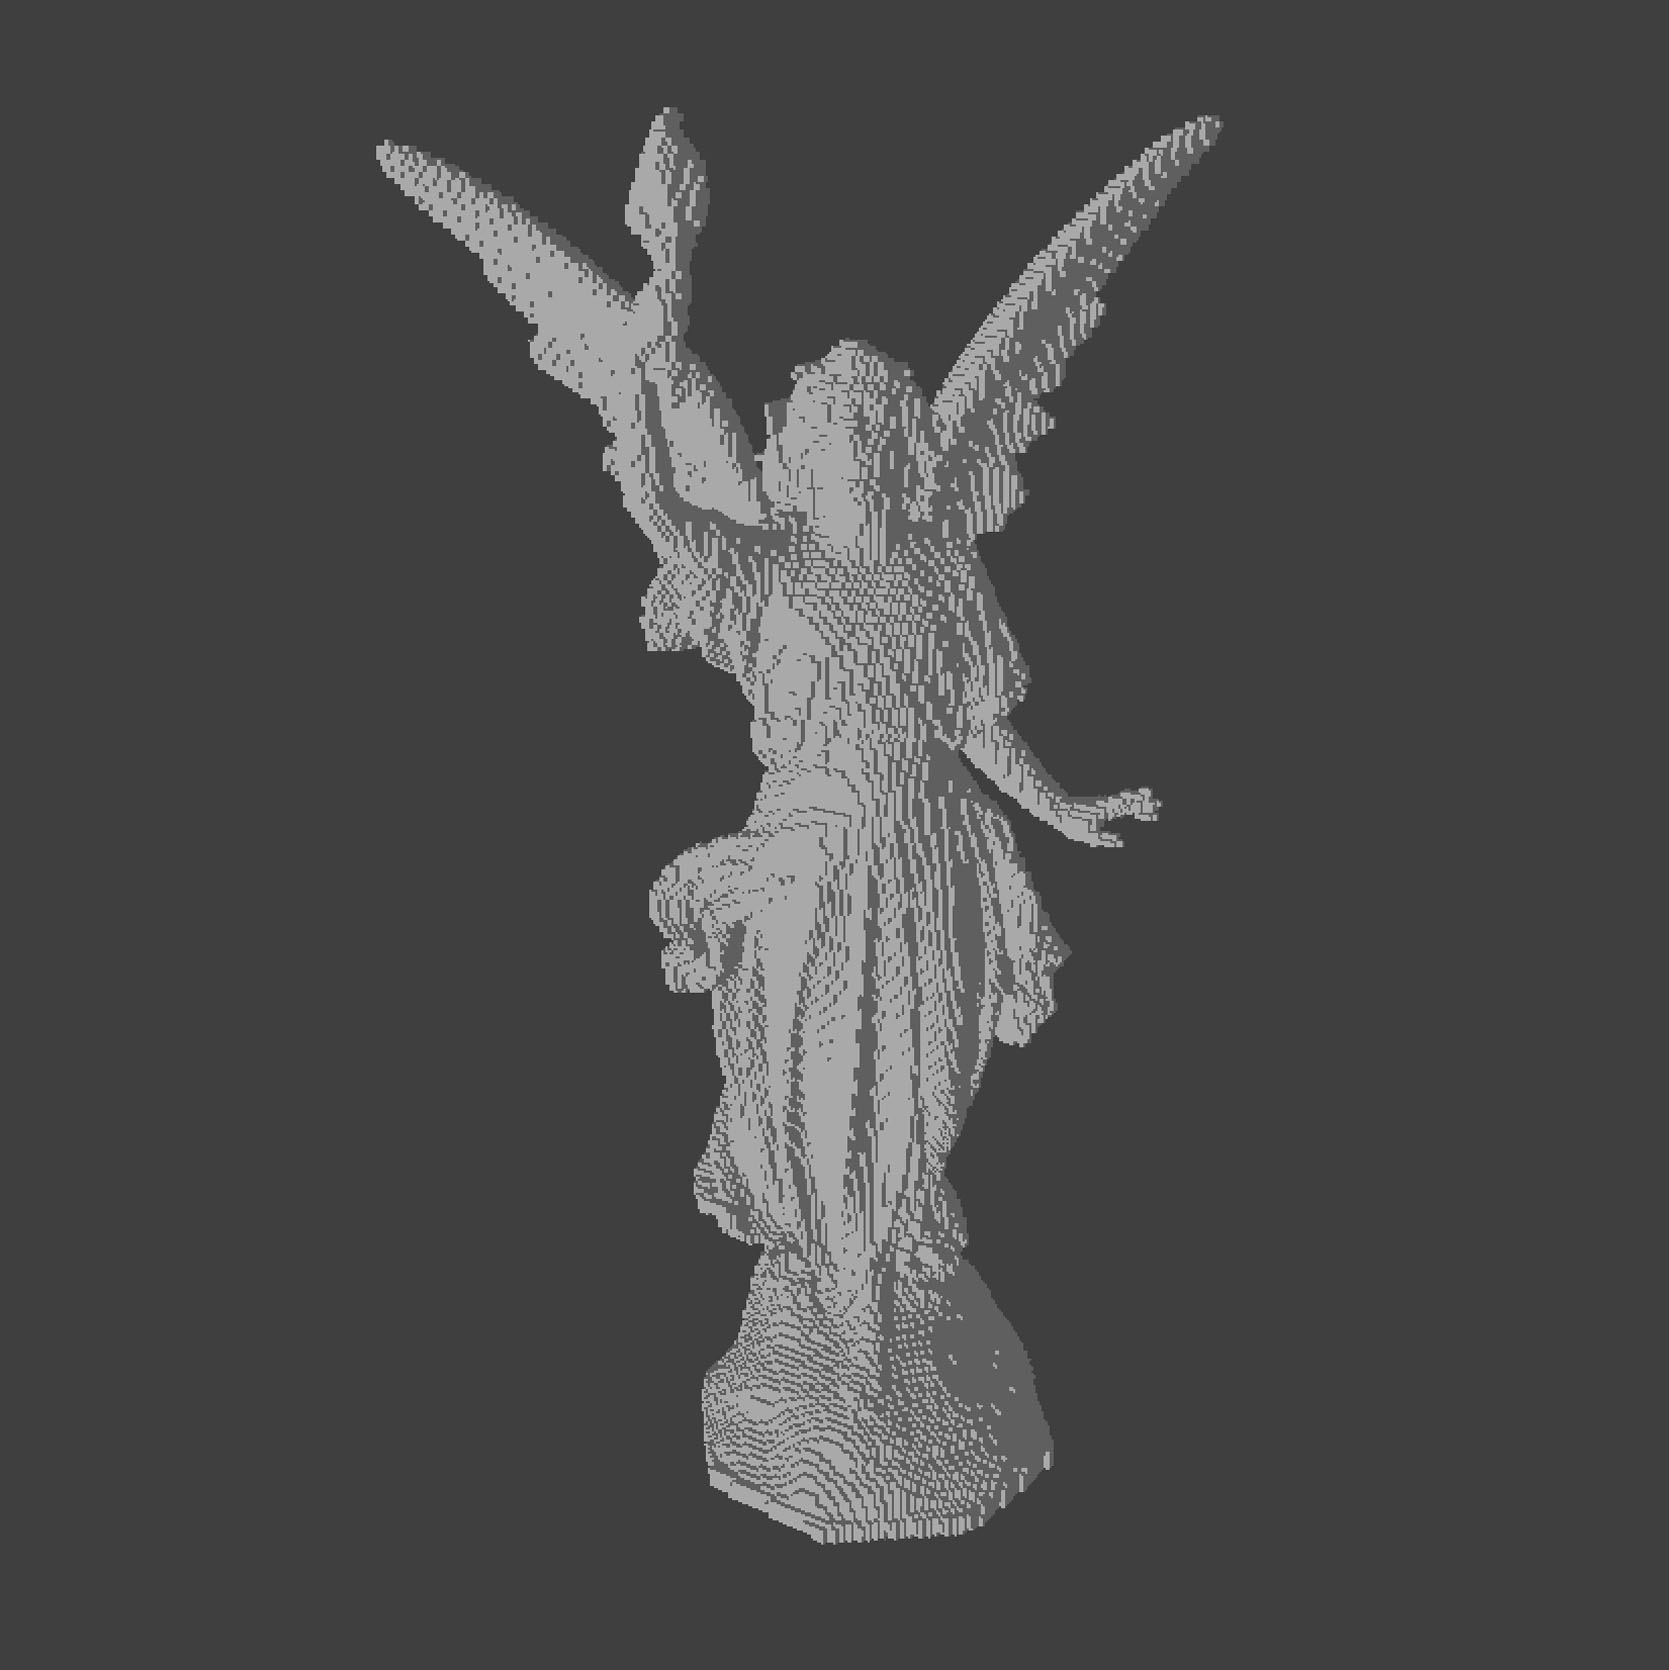
\includegraphics[width=80px]{images/graphics/model-lucy.jpg}
  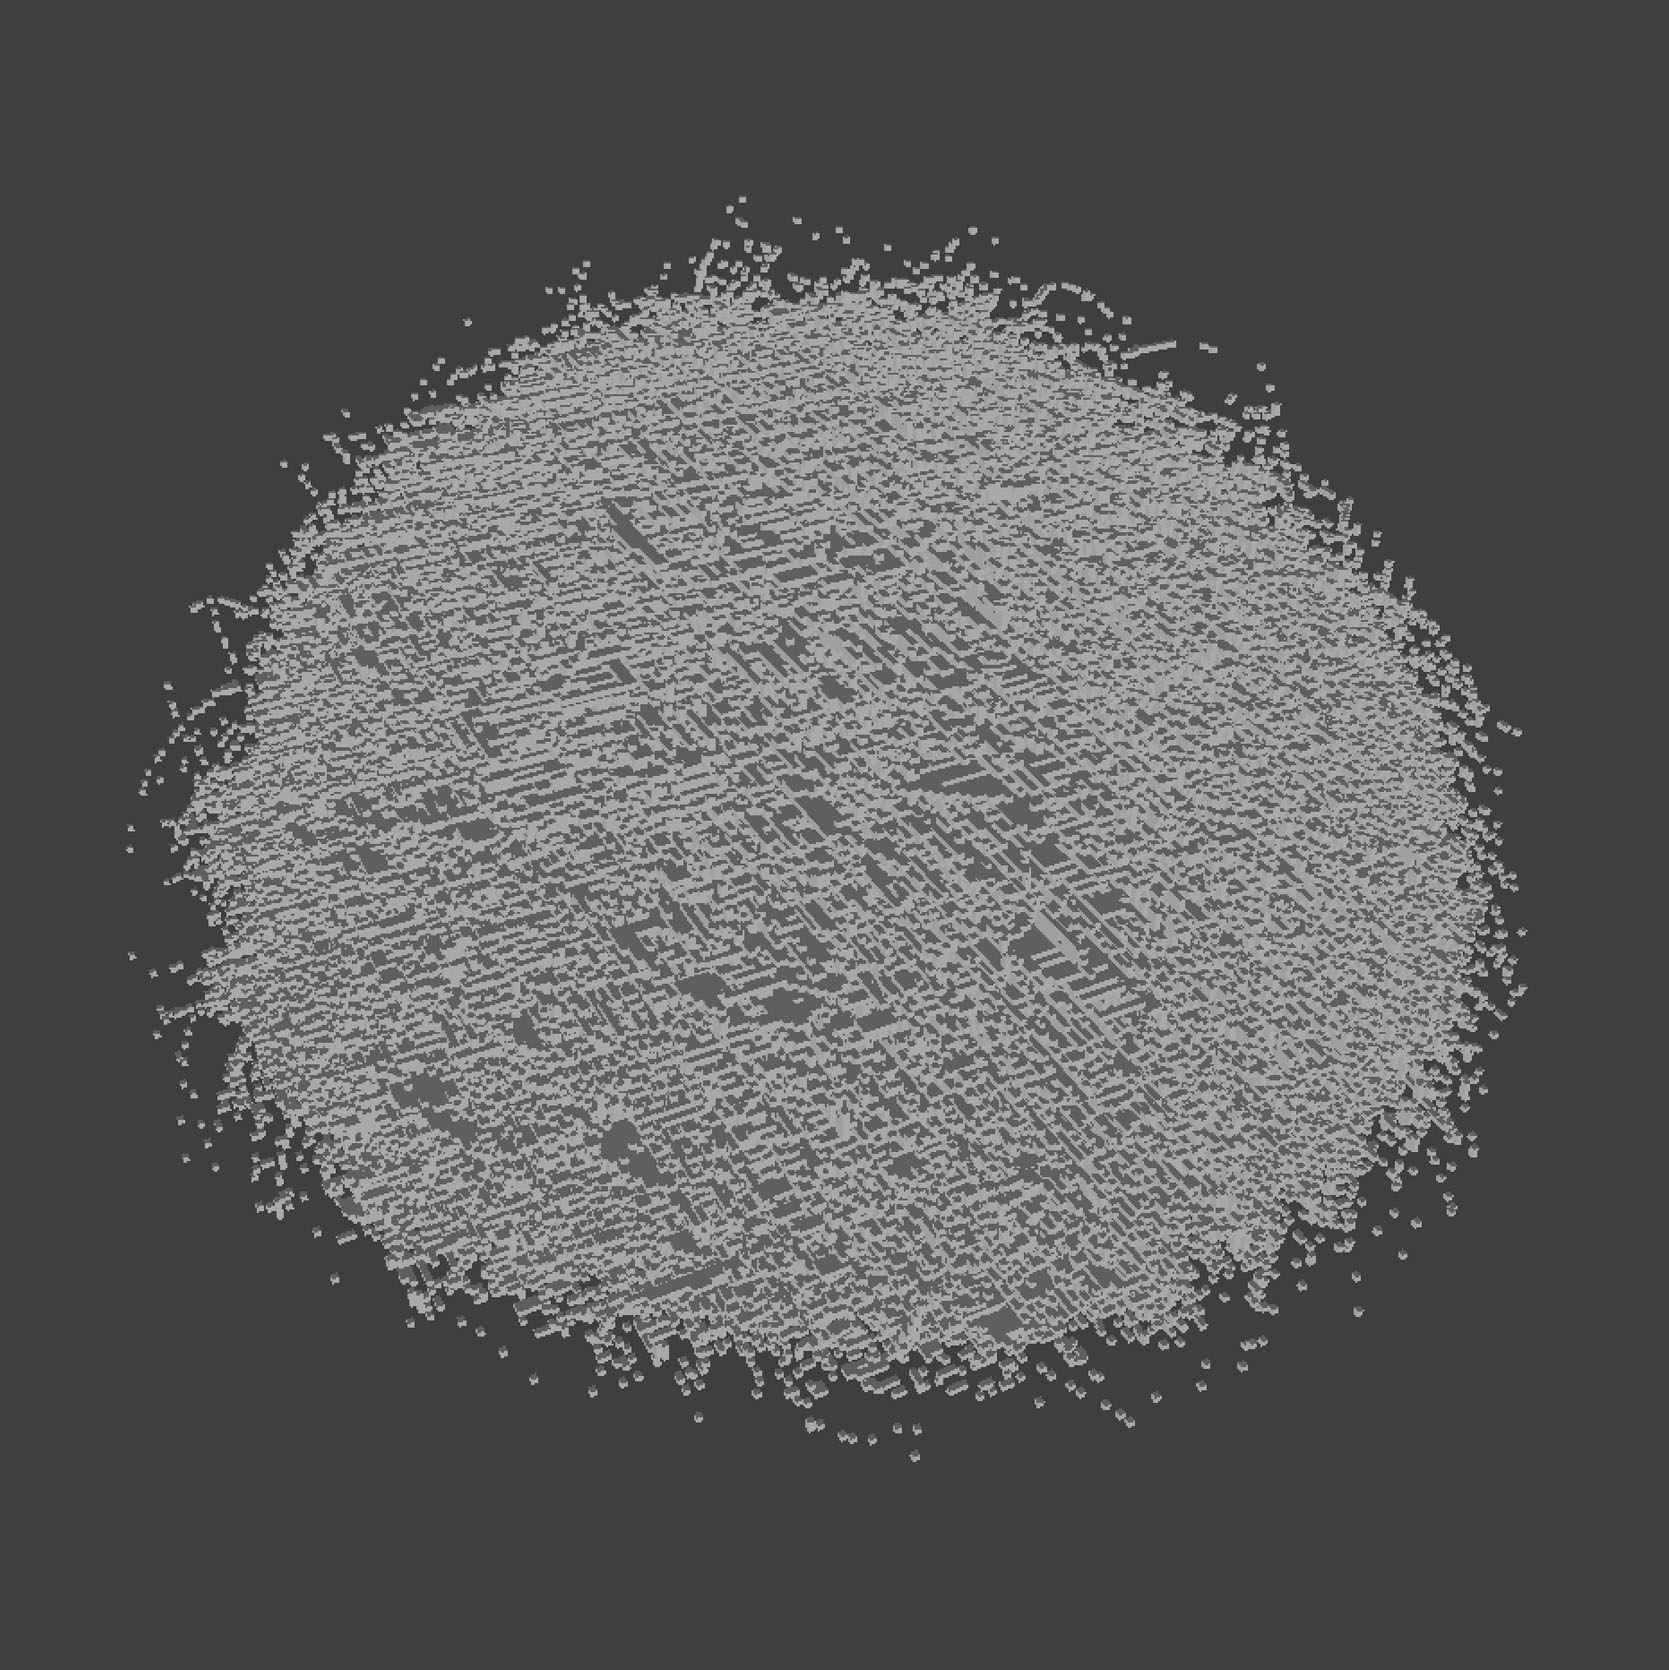
\includegraphics[width=80px]{images/graphics/model-hairball.jpg}
  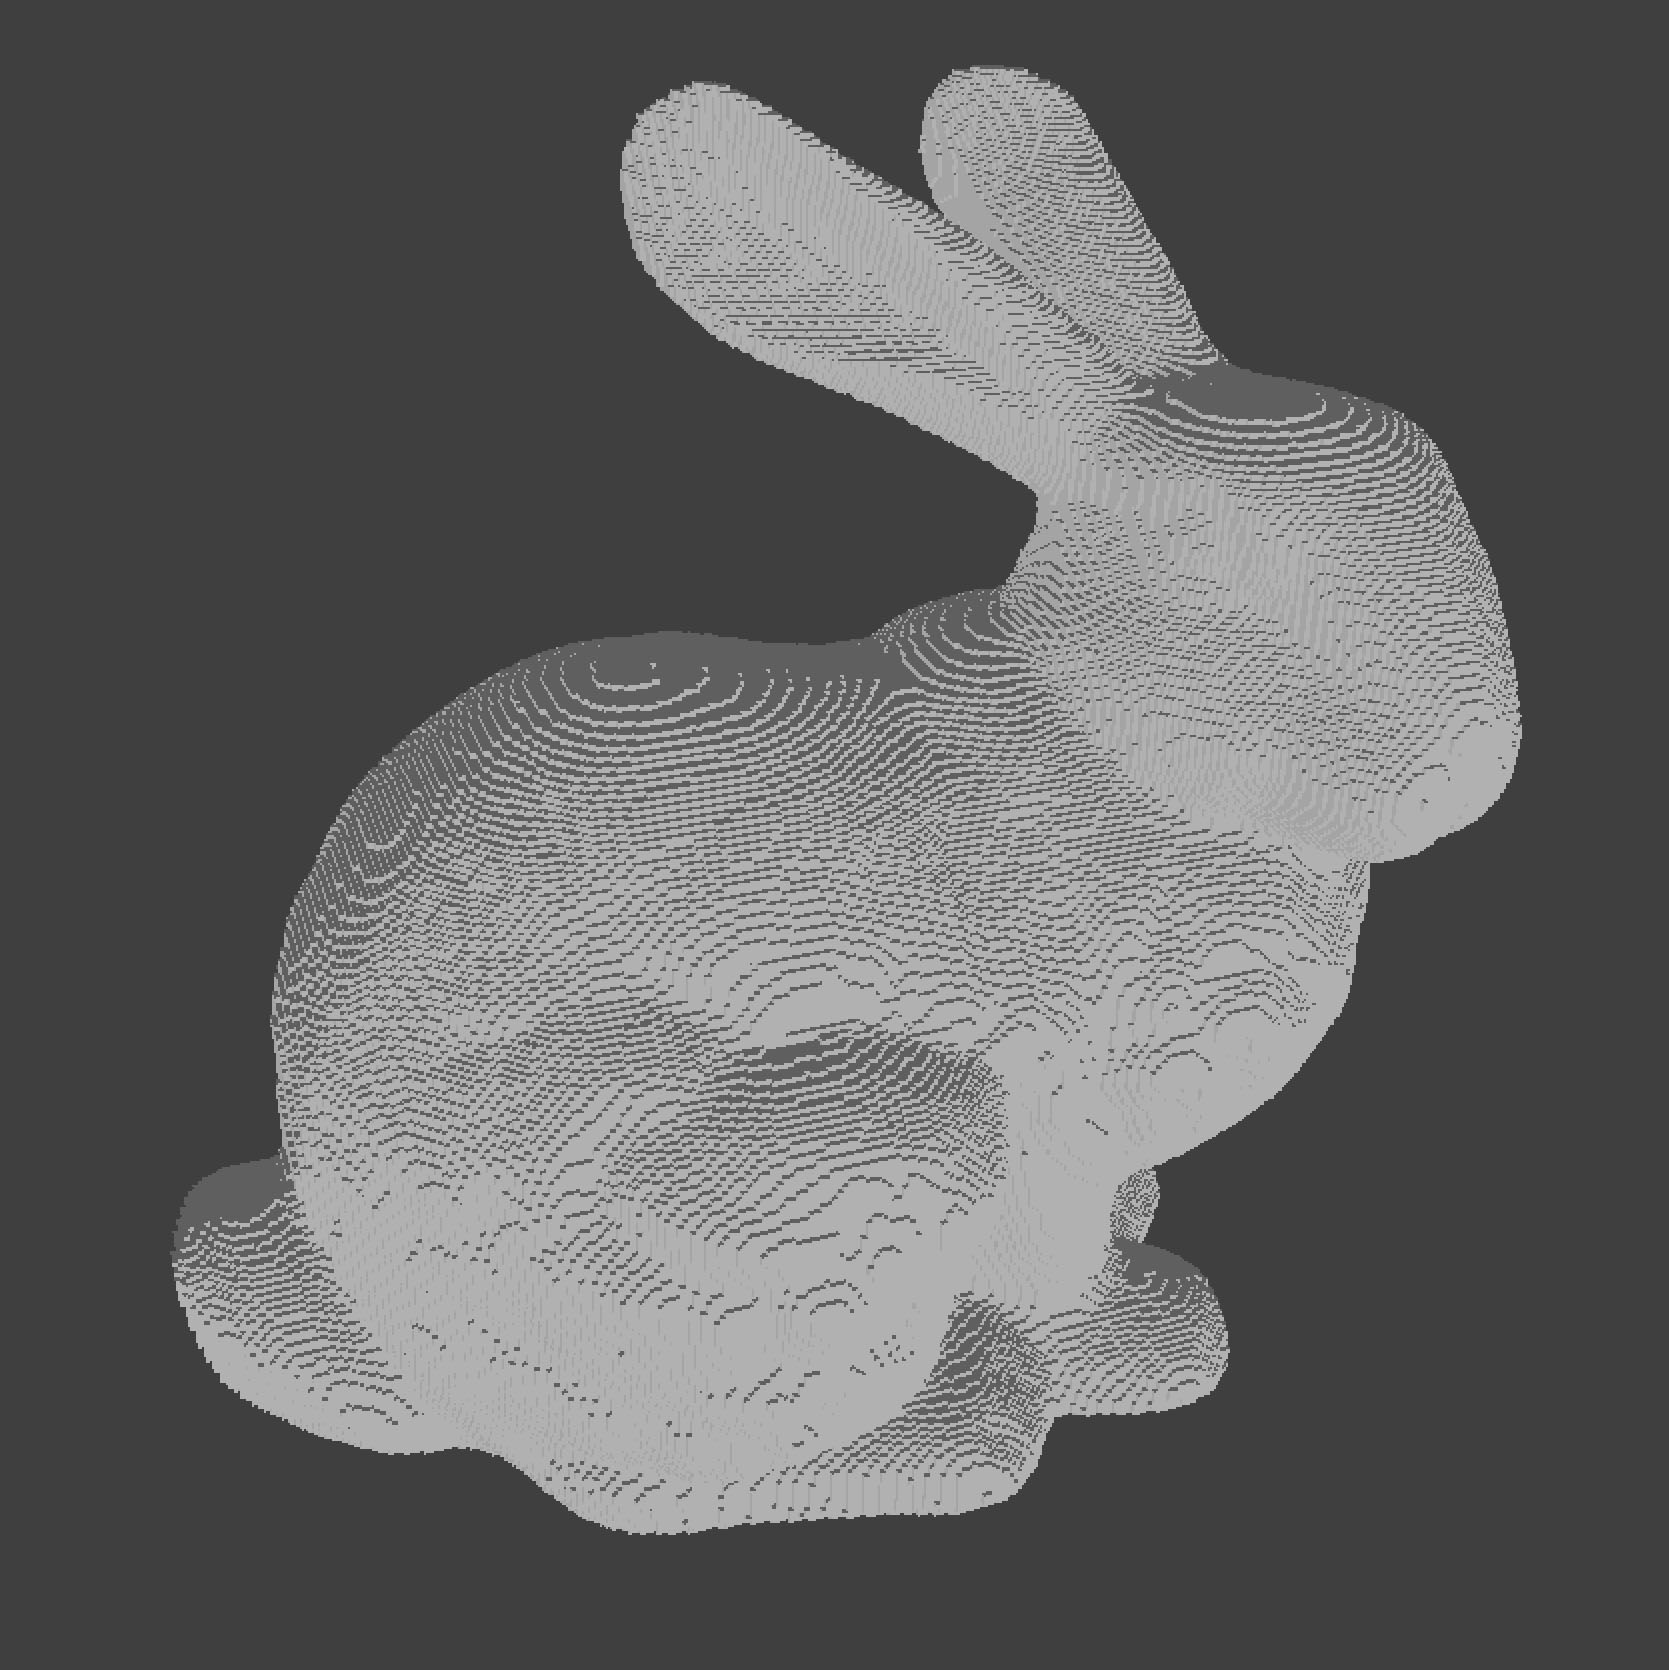
\includegraphics[width=80px]{images/graphics/model-bunny.jpg}
  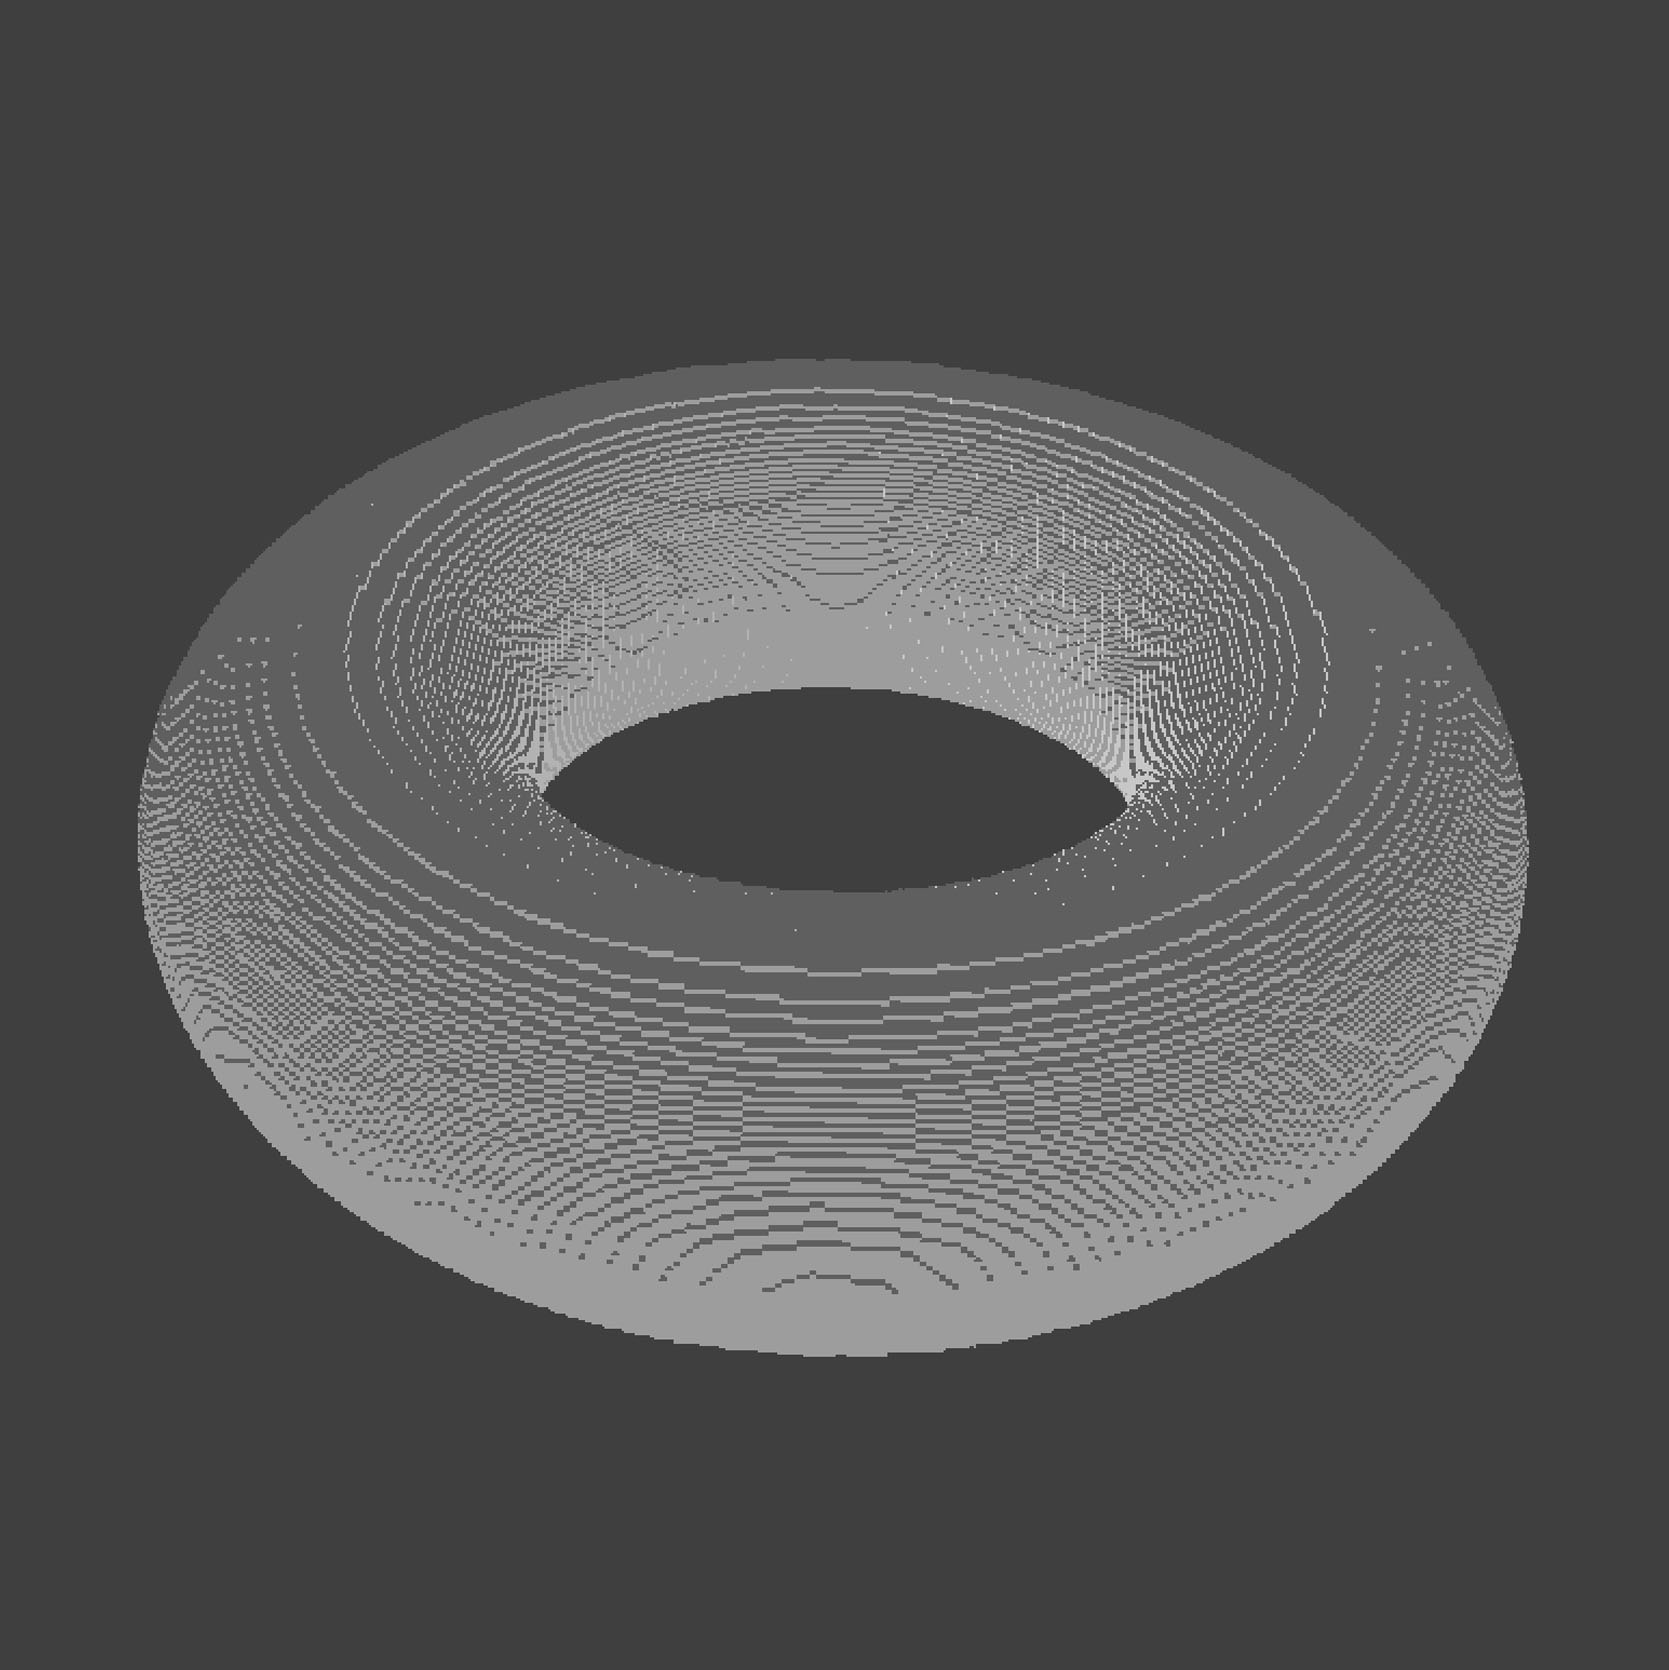
\includegraphics[width=80px]{images/graphics/model-torus.jpg}
  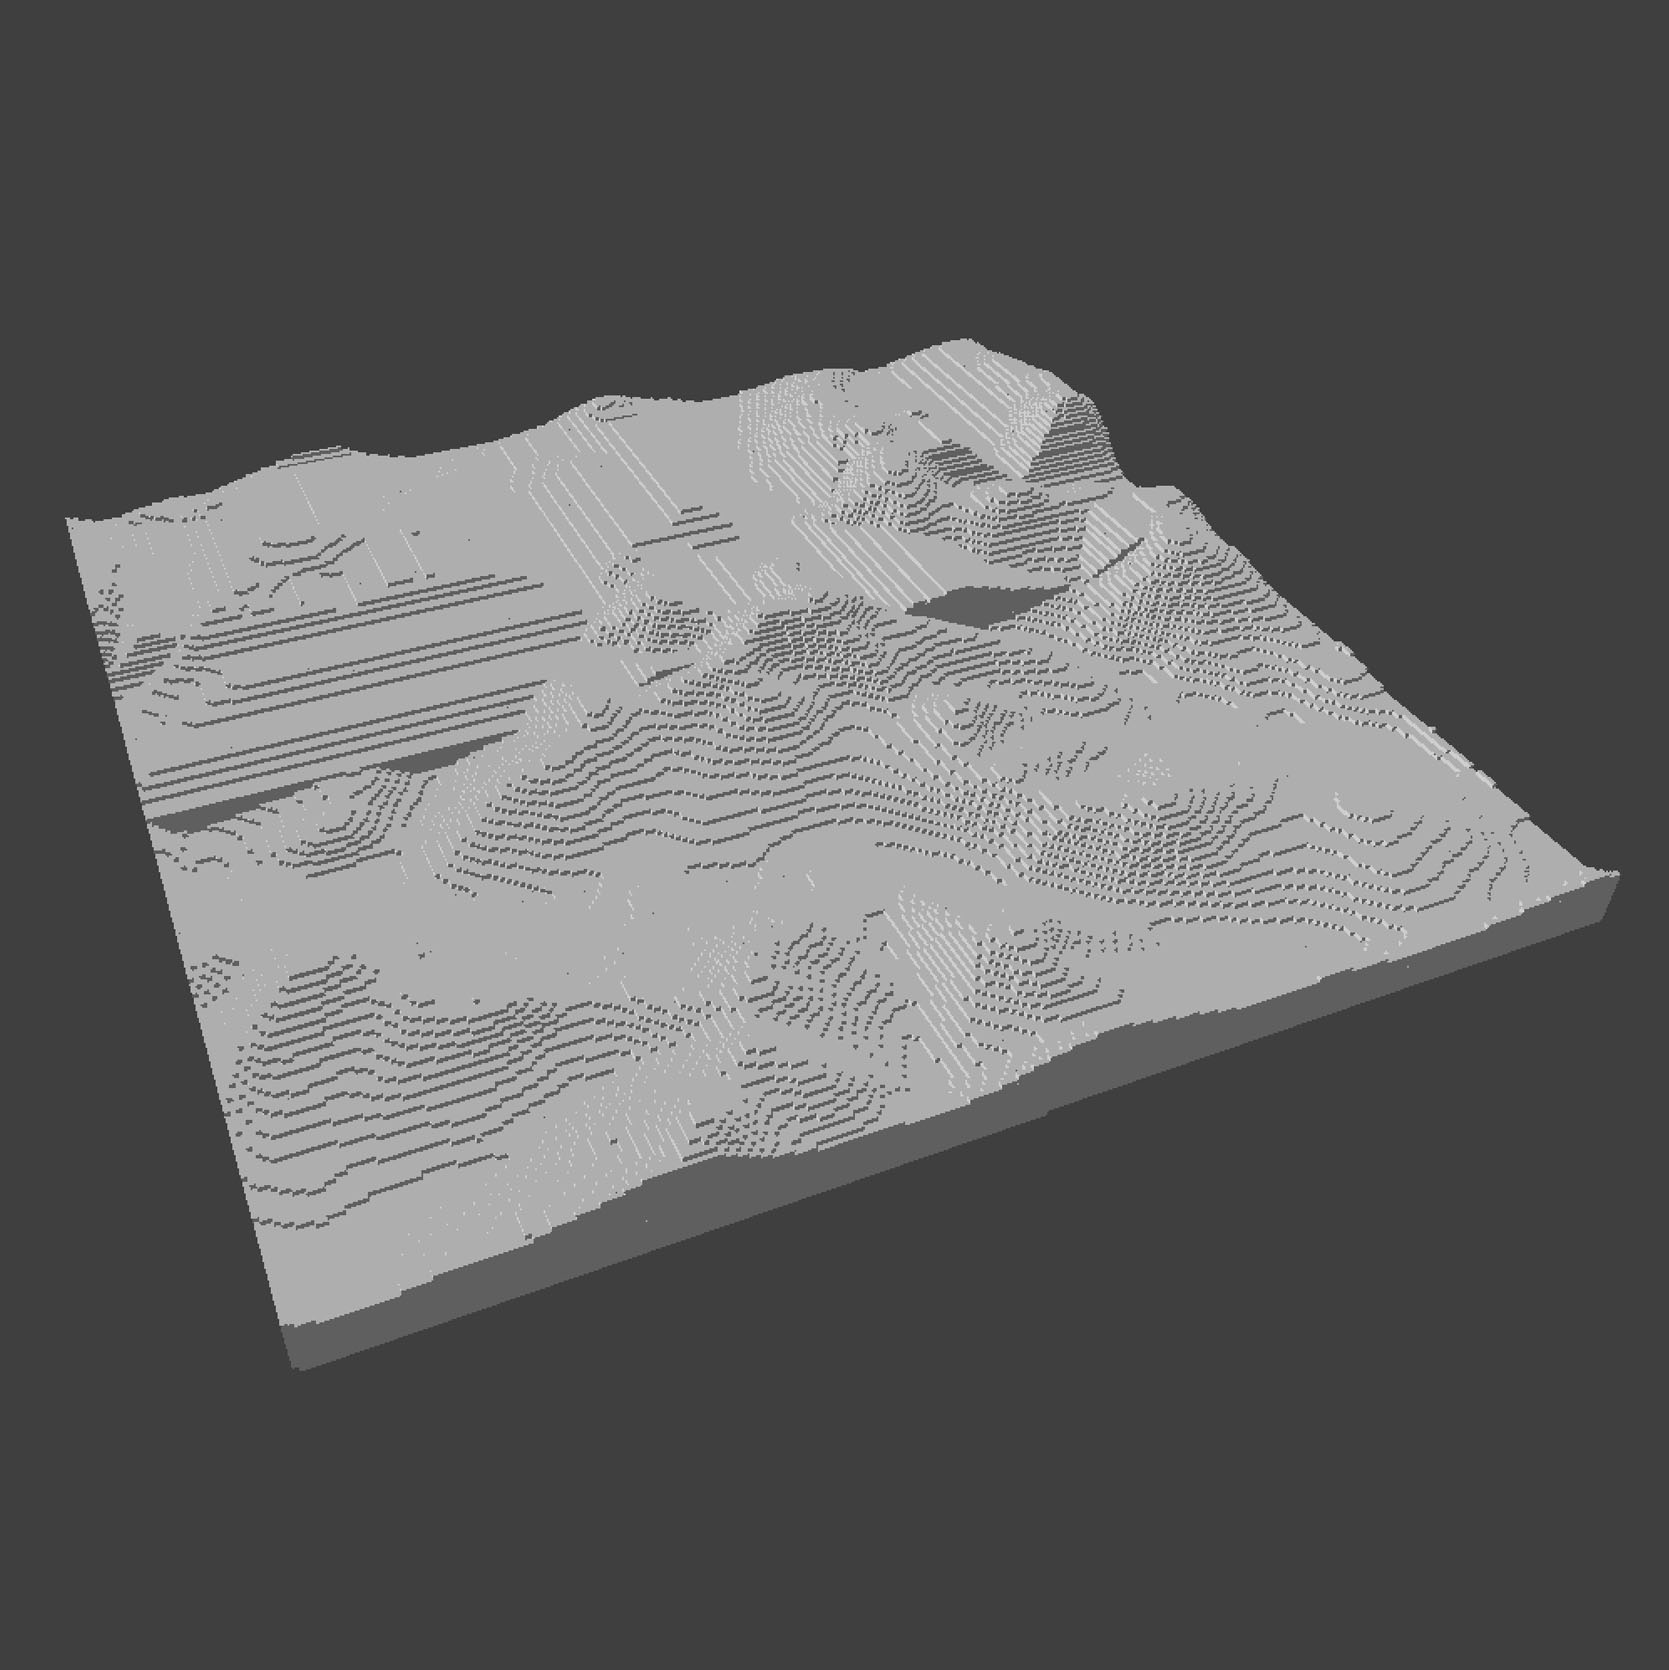
\includegraphics[width=80px]{images/graphics/model-terrain.jpg}
  \caption{The models used for the experiment.}
  \label{fig:experiment-models}
\end{figure}

\noindent
The models that were used in the tests are \emph{Lucy} (Stanford 3D Scanning Repository), the \emph{Stanford Bunny} 
(Stanford 3D Scanning Repository), the \emph{Hairball}, a \emph{Torus} and a \emph{Terrain} scene. All of 
these models provide different characteristics, which tested the pipeline in a variety of ways. \\

\noindent
The \emph{Lucy} model is tall and slim, which means that its volume is distributed more over one axis 
than over the other two axis. This is assumed to provide interesting insights into how such an object 
self-occludes the voxels when viewed from different perspectives. It also has a few narrow parts where 
no best occluders are expected. \\

\noindent
For low resolutions, the \emph{Hairball} isn't voxelized enough to maintain all the thin and tiny details, 
but for higher resolutions, the small structures were assumed to be not sufficient in density to completely
fill octree nodes, resulting in an unfavorable data layout to test the limits of the mesh computations. \\

\noindent
The \emph{Stanford Bunny} is a large and dense model with a lot of voxels in any possible resolution.
It also has different features to it, one of them being the curved surface resulting in a lot of octree 
nodes not being filled completely. On the other hand, because of its large volume, the model is assumed 
to be efficient when rendering the best occluders, aggregating a lot of smaller octree nodes to larger 
approximations. \\ 

\noindent
The \emph{Torus} provides a higher voxel count and a hole in it, which created an area where the 
octree isn't densly filled with voxels. This model was specifically used to test the algorithm's 
capabilities of culling voxels, when the voxels were densly crowded in small parts of the scene, and 
at the same time provided areas with no voxels at all. Also, the \emph{Torus} is an inherently round 
shape and therefore has a lot of partially filled octree nodes representing its surface. \\

\noindent
The \emph{Terrain} model aimed to replicate a relatively flat, open area that could be found in actual 
games like \emph{Minecraft}. Its surface is setup in a way that allows for only a small amount of best 
occluders to be formed. The terrain's hills are assumed to be occluders which again would help for rendering 
such a scene in a game.


%- Compare:
%    - Model turntable rendered without OC
%    - Model turntable rendered with OC
%(   - Model turntable rendered with different OC implementation (? -> hard))
%
%
%- Criteria: 
%    - Frame time
%    - Dispatch numbers (?)
%    - Duration of depth pre-pass
%        - Draw best occluders to depth buffer
%        - Duration of depth hierarchy creation
%    - Visible cubes
%    - Visible octree nodes
%    - Triangle count
%    - Amount of best occluders
%    - CPU time
%    - GPU time
%    - Amount of overdraw (heatmap if possible)
%
%
%- Model variations:
%    - Lucy
%    - Stanford Bunny
%    - Torus (for when objects have "holes")
%    - Some large, wide scenery
%    - Sponza        -> Ehrlich sein und T
%    - ...
%
%
%- Machines:
%    - Laptop
%    - RTX 2080 Ti
%    - RTX 4090
%    - Multiple devices


\section{Experimental Results}

In this section the experimental results are presented and discussed for each model tested.
For each model the culling results are presented, which includes data that isn't dependent 
on specific hardware. After that, the profiling measurements are discussed, which relate to 
the hardware setup presented in \ref{subsec-experimental-environment}. 

\subsection*{Stanford Lucy}

 \subsubsection*{Culling Results}

% --------------------------------------- LUCY 256 ---------------------------------------

\begin{figure}[h]              % Lucy 256 Voxels Test Anim
    \begin{center}
      \begin{tikzpicture}
        \begin{axis}[
            width=\linewidth, % Scale the plot to \linewidth
            height=100px,
            xlabel={Frames},
            ylabel={Visible Voxels},
            grid,
            xmin=0,
            xmax=2392,
            ymin=60000,
            ymax=160000
          ]
          \addplot[green, no marks, solid] table[col sep=comma, x=frame, y=visible_voxels]{./plotdata/lucy_256_voxels.csv};
          \addplot[blue, dotted, no marks, domain=0:2393, samples=50] {140842};
          \addplot[orange, no marks, solid] table[col sep=comma, x=frame, y=visible_voxels]{./plotdata/lucy_256_voxels_pmoc.csv};
          \addplot[red, dotted, no marks, domain=0:2393, samples=50] {84082};
        \end{axis}
      \end{tikzpicture}
      \caption{The amount of visible voxels over the course of the test animation shown in green for 
      per-octree occlusion culling, and in orange for per-meshlet occlusion culling. 
      The average amount of visible voxels was \emph{140,842} for per-octree occlusion culling, which is 
      marked as the blue dotted line, and \emph{84,082} for per-meshlet occlusion culling, marked in red.}
      \label{plt:lucy-256-culling-res-voxels}
    \end{center}
  \end{figure}


  \begin{figure}[h]            % Lucy 256 OT Nodes Test Anim
    \begin{center}
      \begin{tikzpicture}
        \begin{axis}[
            width=\linewidth, % Scale the plot to \linewidth
            height=100px,
            xlabel={Frames},
            ylabel={Visible Nodes},
            grid,
            xmin=0,
            xmax=2392,
            ymin=1800,
            ymax=4000
          ]
          \addplot[green, no marks, solid] table[col sep=comma, x=frame, x expr=\thisrow{frame} * 2392 / 2392, y=visible_nodes]{./plotdata/lucy_256_nodes.csv};
          \addplot[blue, dotted, no marks, domain=0:2393, samples=50] {3460};
          \addplot[orange, no marks, solid] table[col sep=comma, x=frame, x expr=\thisrow{frame} * 2392 / 2395, y=visible_nodes]{./plotdata/lucy_256_nodes_pmoc.csv};
          \addplot[red, dotted, no marks, domain=0:2393, samples=50] {2483};
        \end{axis}
      \end{tikzpicture}
      \caption{The amount of visible octree nodes over the course of the test animation shown in green for 
      per-octree occlusion culling and in orange for per-meshlet occlusion culling. 
      The average amount of visible octree nodes was \emph{3,460} for per-octree occlusion culling, which is 
      marked as the blue dotted line, and \emph{2,483} for per-meshlet occlusion culling, which is marked in 
      as the red dotted line.}
      \label{plt:lucy-256-culling-res-nodes}
    \end{center}
  \end{figure}

% ----------------------------------------------------------------------------------------

\noindent
Figures \ref{plt:lucy-256-culling-res-voxels} and \ref{plt:lucy-256-culling-res-nodes} show the 
amount of visible voxels and visible octree nodes for both the per-octree meshlet culling and the 
per-meshlet octree culling configuration. The measurements were directly sampled from the 
\emph{Task Shader} over the course of the testing animation. Figure \ref{plt:lucy-256-culling-res-voxels}
presents the amount of visible voxels while figure \ref{plt:lucy-256-culling-res-nodes} shows the amount 
of visible octree nodes. Both values directly correlate since culled octree nodes result in culled voxels.
The per-octree occlusion culling configuration is shown in green, with a dotted blue line representing the 
average value over time. The orange graph shows the per-meshlet occlusion culling configuration, and an 
additional red dotted line representing the average values for this configuration. The respective graphs for 
the other models follow the same color code. [@TODO: Consider moving analysis out of per model text]\\


\noindent
It is obvious that the per-meshlet culling 
significantly reduced the amount of dispatched voxels and octree nodes, which lead to less load for the 
rasterizer and the pixel shader. The amount of octree nodes decreased when using per-meshlet culling, because 
octree nodes could be culled, even when their corners were visible by the camera. For instance, when considering 
a node that holds just 5 voxels, which are all overlapped by a part of the model, this octree node will be 
inherently culled when using per-meshlet culling. Contrary, when using per-octree culling, the culling is 
dependant on the visibility of any of the octree nodes corners, which can result in a node being not culled, 
even though all voxels within that node remain occluded. \\

\noindent 
Both curves indicate how the model fits the overall culling algorithm. For instance, the \emph{Stanford Lucy} 
model has a relatively even curve over time. Of course, this is a dynamic measure and highly depends on the 
angle of the camera. Still, the compact, tall model provides a good amount of best occluders to occlude a 
relatively even number of voxels when viewed from the side. \\

\noindent
Considering the average amount of visible voxels, the per-octree algorithm was able to cull $57.5\%$ of all 
voxels. The per-meshlet culling even managed to ommit on average $74.6\%$ of all voxels. 


\subsubsection*{Performance Results}

% CPU performance


% GPU performance

\begin{figure}
  \centering
  \begin{tikzpicture}
    \begin{axis}[
      xbar stacked,
      xmin=0,
      width=\textwidth,
      height=5cm,
      ytick=data,
      bar width=10pt,
      xlabel={Time (us)},
      symbolic y coords={Lucy4, Lucy3, Lucy2, Lucy1, Lucy0},
      ytick=data,
      legend style={at={(0.5,1.1)}, anchor=south, legend columns=-1}
    ]

    \addplot [fill=green!80]  table [col sep=comma, x=DepthPrepass, y=Label]  {plotdata/gpu/lucy_gpu_profiling_frame_pooc.csv};
    \addplot [fill=blue!60]   table [col sep=comma, x=DispatchMesh, y=Label]  {plotdata/gpu/lucy_gpu_profiling_frame_pooc.csv};
    \addplot [fill=orange!60] table [col sep=comma, x=Misc,         y=Label]  {plotdata/gpu/lucy_gpu_profiling_frame_pooc.csv};

    \legend{Depth Prepass, Dispatch Mesh, Miscellaneous}
    \end{axis}
  \end{tikzpicture}
  \caption{The complete time measured on the \ac{GPU}. The \emph{Depth Prepass} is the extra overhead introduced 
  by the \ac{HZB}. The \emph{Dispatch Mesh} is the drawing of the meshes, including the occlusion culling. 
  \emph{Miscellaneous} includes a small amount of \emph{barriers} used for synchronisation and the rendering 
  of some debug \ac{UI}. It is considered to be more or less static in computation time and is not part of 
  the actual algorithm measured in this experiment.}
\end{figure}




\begin{figure}
  \centering
  \begin{tikzpicture}
    \begin{axis}[
      xbar stacked,
      xmin=0,
      width=\textwidth,
      height=5cm,
      ytick=data,
      bar width=10pt,
      xlabel={Time (us)},
      symbolic y coords={Lucy4, Lucy3, Lucy2, Lucy1, Lucy0},
      ytick=data,
      legend style={at={(0.5,1)}, anchor=north, legend columns=-1}
    ]

    \addplot [fill=red!80]    table [col sep=comma, x=DispatchBestOccluders,  y=Label]  {plotdata/gpu/lucy_gpu_profiling_prepass_pooc.csv};
    \addplot [fill=pink!60]   table [col sep=comma, x=CopyTex,                y=Label]  {plotdata/gpu/lucy_gpu_profiling_prepass_pooc.csv};
    \addplot [fill=yellow!60] table [col sep=comma, x=GenMipChain,            y=Label]  {plotdata/gpu/lucy_gpu_profiling_prepass_pooc.csv};

    \legend{Dispatch Best Occluders, Copy Depth Buffer, Generate HiZ-Pyramid}
    \end{axis}
  \end{tikzpicture}
  \caption{The time measured in the \emph{Depth Prepass}. The \emph{Dispatch Best Occluders} is the drawing to the 
  depth buffer. The \emph{Copy Depth Buffer} computation copies the depth buffers content into the final \ac{HiZ} resource.
  Finally, \emph{Generate HiZ-Pyramid} shows the \ac{HiZ} creation, which is done sequentially.}
\end{figure}



\subsection*{Stanford Bunny}


% --------------------------------------- BUNNY 256 --------------------------------------

\begin{figure}[h]              % Bunny 256 Voxels Test Anim
    \begin{center}
      \begin{tikzpicture}
        \begin{axis}[
            width=\linewidth, % Scale the plot to \linewidth
            height=100px,
            xlabel={Frames},
            ylabel={Visible Voxels},
            grid,
            xmin=0,
            xmax=1186,
            ymin=100000,
            ymax=500000
          ]
          \addplot[green, no marks, solid] table[col sep=comma, x=frame, x expr=\thisrow{frame} * 1186 / 1186, y=visible_voxels]{plotdata/bunny_256_voxels.csv};
          \addplot[blue, dotted, no marks, domain=0:1186, samples=50] {385210};
          \addplot[orange, no marks, solid] table[col sep=comma, x=frame, x expr=\thisrow{frame} * 1186 / 1490, y=visible_voxels]{plotdata/bunny_256_voxels_pmoc.csv};
          \addplot[red, dotted, no marks, domain=0:1186, samples=50] {180266};
        \end{axis}
      \end{tikzpicture}
      \caption{The amount of visible voxels over the course of the test animation shown in green for 
      per-octree occlusion culling, and in orange for per-meshlet occlusion culling. 
      The average amount of visible voxels was \emph{385,210} for per-octree occlusion culling, which is 
      marked as the blue dotted line, and \emph{180,266} for per-meshlet occlusion culling, marked in red.}
      \label{plt:bunny-256-culling-res-voxels}
    \end{center}
  \end{figure}

  \begin{figure}[h]            % Bunny 256 OT Nodes Test Anim
    \begin{center}
      \begin{tikzpicture}
        \begin{axis}[
            width=\linewidth, % Scale the plot to \linewidth
            height=100px,
            xlabel={Frames},
            ylabel={Visible Nodes},
            grid,
            xmin=0,
            xmax=1186,
            ymin=3000,
            ymax=10000
          ]
          \addplot[green, no marks, solid] table[col sep=comma, x=frame, x expr=\thisrow{frame} * 1186 / 1186, y=visible_nodes]{./plotdata/bunny_256_nodes.csv};
          \addplot[blue, dotted, no marks, domain=0:1186, samples=50] {8519};
          \addplot[orange, no marks, solid] table[col sep=comma, x=frame, x expr=\thisrow{frame} * 1186 / 1490, y=visible_nodes]{./plotdata/bunny_256_nodes_pmoc.csv};
          \addplot[red, dotted, no marks, domain=0:1186, samples=50] {5415};
        \end{axis}
      \end{tikzpicture}
      \caption{The amount of visible octree nodes over the course of the test animation shown in green for 
      per-octree occlusion culling and in orange for per-meshlet occlusion culling. 
      The average amount of visible octree nodes was \emph{8,519} for per-octree occlusion culling, which is 
      marked as the blue dotted line, and \emph{5,415} for per-meshlet occlusion culling, which is marked in 
      as the red dotted line.}
      \label{plt:bunny-256-culling-res-nodes}
    \end{center}
  \end{figure}
 
% ----------------------------------------------------------------------------------------

\noindent
Similar to the first model, the \emph{Stanford Bunny} also discards a significant amount of 
voxels in both of the applied culling configurations. The average culling ratio was $88.6\%$ 
for the per-octree occlusion culling, and $94.6\%$ for the per-meshlet culling. This immense 
amount of occlusion is due to the already large amount of \emph{3,379,738} total voxels in the 
mesh and the large volume of the model, which provides a good basis for the generation of best 
occluders. \\



\subsection*{Torus - $256^3$}

% --------------------------------------- TORUS 256 --------------------------------------

\begin{figure}[h]              % Torus 256 Voxels Test Anim
    \begin{center}
      \begin{tikzpicture}
        \begin{axis}[
            width=\linewidth, % Scale the plot to \linewidth
            height=100px,
            xlabel={Frames},
            ylabel={Visible Voxels},
            grid,
            xmin=0,
            xmax=1087,
            ymin=70000,
            ymax=500000
          ]
          \addplot[green, no marks, solid] table[col sep=comma, x=frame, x expr=\thisrow{frame} * 1087 / 1087, y=visible_voxels]{./plotdata/torus_256_voxels.csv};
          \addplot[blue, dotted, no marks, domain=0:1087, samples=50] {359313};
          \addplot[orange, no marks, solid] table[col sep=comma, x=frame, x expr=\thisrow{frame} * 1087 / 1845, y=visible_voxels]{./plotdata/torus_256_voxels_pmoc.csv};
          \addplot[red, dotted, no marks, domain=0:1087, samples=50] {170772};
        \end{axis}
      \end{tikzpicture}
      \caption{The amount of visible voxels over the course of the test animation shown in green for 
      per-octree occlusion culling, and in orange for per-meshlet occlusion culling. 
      The average amount of visible voxels was \emph{359,313} for per-octree occlusion culling, which is 
      marked as the blue dotted line, and \emph{170,772} for per-meshlet occlusion culling, marked in red.}
      \label{plt:torus-256-culling-res-voxels}
    \end{center}
  \end{figure}


  \begin{figure}[h]            % Torus 256 OT Nodes Test Anim
    \begin{center}
      \begin{tikzpicture}
        \begin{axis}[
            width=\linewidth, % Scale the plot to \linewidth
            height=100px,
            xlabel={Frames},
            ylabel={Visible Nodes},
            grid,
            xmin=0,
            xmax=1087,
            ymin=1000,
            ymax=10000
          ]
          \addplot[green, no marks, solid] table[col sep=comma, x=frame, x expr=\thisrow{frame} * 1087 / 1087, y=visible_nodes]{./plotdata/torus_256_nodes.csv};
          \addplot[blue, dotted, no marks, domain=0:1087, samples=50] {7712};
          \addplot[orange, no marks, solid] table[col sep=comma, x=frame, x expr=\thisrow{frame} * 1087 / 1845, y=visible_nodes]{./plotdata/torus_256_nodes_pmoc.csv};
          \addplot[red, dotted, no marks, domain=0:1087, samples=50] {4768};
        \end{axis}
      \end{tikzpicture}
      \caption{The amount of visible octree nodes over the course of the test animation shown in green for 
      per-octree occlusion culling and in orange for per-meshlet occlusion culling. 
      The average amount of visible octree nodes was \emph{7,712} for per-octree occlusion culling, which is 
      marked as the blue dotted line, and \emph{4,768} for per-meshlet occlusion culling, which is marked in 
      as the red dotted line.}
      \label{plt:torus-256-culling-res-nodes}
    \end{center}
  \end{figure}

% ----------------------------------------------------------------------------------------

\noindent
The \emph{Torus} model varied in culling efficiency depending on the view angle. As expected, the hole 
in the mesh turned out to be inefficient for the culling algorithm. When considering the occlusion ratio, 
both the per-octree occlusion culling and the oer-meshlet occlusion culling performed significantly better 
when the torus was viewed from an angle, occluding the hole in the middle. The variation between the maxium 
amount of visible voxels and the minimum amount of voxels was the highest for the \emph{Torus} model, which 
is remarkable compared to the other models. Using this particular experimental setup, the lowest amount of 
visible voxels was $36.8\%$ of the maximum amount of visible voxels. This variation is also clearly evident 
in figure \ref{plt:torus-256-culling-res-voxels}. \\ 

\noindent
In general, for per-octree culling, the average culling ratio was $84.4\%$, and $92.6\%$ for per-meshlet culling. 



\subsection*{Terrain - $256^3$}

% -------------------------------------- TERRAIN 256 -------------------------------------

\begin{figure}[h]              % Terrain 256 Voxels Test Anim
    \begin{center}
      \begin{tikzpicture}
        \begin{axis}[
            width=\linewidth, % Scale the plot to \linewidth
            height=100px,
            xlabel={Frames},
            ylabel={Visible Voxels},
            grid,
            xmin=0,
            xmax=1239,
            ymin=70000,
            ymax=500000
          ]
          \addplot[green, no marks, solid] table[col sep=comma, x=frame, x expr=\thisrow{frame} * 1239 / 1239, y=visible_voxels]{./plotdata/terrain_256_voxels.csv};
          \addplot[blue, dotted, no marks, domain=0:1239, samples=50] {396228};
          \addplot[orange, no marks, solid] table[col sep=comma, x=frame, x expr=\thisrow{frame} * 1239 / 1759, y=visible_voxels]{./plotdata/terrain_256_voxels_pmoc.csv};
          \addplot[red, dotted, no marks, domain=0:1239, samples=50] {180440};
        \end{axis}
      \end{tikzpicture}
      \caption{The amount of visible voxels over the course of the test animation shown in green for 
      per-octree occlusion culling, and in orange for per-meshlet occlusion culling. 
      The average amount of visible voxels was \emph{396,228} for per-octree occlusion culling, which is 
      marked as the blue dotted line, and \emph{180,440} for per-meshlet occlusion culling, marked in red.}
      \label{plt:terrain-256-culling-res-voxels}
    \end{center}
  \end{figure}


  \begin{figure}[h]            % Terrain 256 OT Nodes Test Anim
    \begin{center}
      \begin{tikzpicture}
        \begin{axis}[
            width=\linewidth, % Scale the plot to \linewidth
            height=100px,
            xlabel={Frames},
            ylabel={Visible Nodes},
            grid,
            xmin=0,
            xmax=1239,
            ymin=1000,
            ymax=10000
          ]
          \addplot[green, no marks, solid] table[col sep=comma, x=frame, x expr=\thisrow{frame} * 1239 / 1239, y=visible_nodes]{./plotdata/terrain_256_nodes.csv};
          \addplot[blue, dotted, no marks, domain=0:1239, samples=50] {8207};
          \addplot[orange, no marks, solid] table[col sep=comma, x=frame, x expr=\thisrow{frame} * 1239 / 1759, y=visible_nodes]{./plotdata/terrain_256_nodes_pmoc.csv};
          \addplot[red, dotted, no marks, domain=0:1239, samples=50] {3832};
        \end{axis}
      \end{tikzpicture}
      \caption{The amount of visible octree nodes over the course of the test animation shown in green for 
      per-octree occlusion culling and in orange for per-meshlet occlusion culling. 
      The average amount of visible octree nodes was \emph{8,207} for per-octree occlusion culling, which is 
      marked as the blue dotted line, and \emph{3,832} for per-meshlet occlusion culling, which is marked in 
      as the red dotted line.}
      \label{plt:terrain-256-culling-res-nodes}
    \end{center}
  \end{figure}

% ----------------------------------------------------------------------------------------


\noindent
The terrain model shows a rather stable occlusion over time, with a ratio of about $58.4\%$ culled voxels 
using the per-octree culling configuration, and about $81.1\%$ voxels being culled in the per-meshlet 
configuration. 



\subsection*{Terrain - $256^3$}

% -------------------------------------- HAIRBALL 256 -------------------------------------

\begin{figure}[h]              % Hairball 256 Voxels Test Anim
    \begin{center}
      \begin{tikzpicture}
        \begin{axis}[
            width=\linewidth, % Scale the plot to \linewidth
            height=100px,
            xlabel={Frames},
            ylabel={Visible Voxels},
            grid,
            xmin=0,
            xmax=940,
            ymin=450000,
            ymax=850000
          ]
          \addplot[green, no marks, solid] table[col sep=comma, x=frame, x expr=\thisrow{frame} * 940 / 940, y=visible_voxels]{./plotdata/hairball_256_voxels.csv};
          \addplot[blue, dotted, no marks, domain=0:940, samples=50] {697549};
          \addplot[orange, no marks, solid] table[col sep=comma, x=frame, x expr=\thisrow{frame} * 940 / 1187, y=visible_voxels]{./plotdata/hairball_256_voxels_pmoc.csv};
          \addplot[red, dotted, no marks, domain=0:940, samples=50] {0};
        \end{axis}
      \end{tikzpicture}
      \caption{The amount of visible voxels over the course of the test animation shown in green for 
      per-octree occlusion culling, and in orange for per-meshlet occlusion culling. 
      The average amount of visible voxels was \emph{697,549} for per-octree occlusion culling, which is 
      marked as the blue dotted line, and \emph{0} for per-meshlet occlusion culling, marked in red.}
      \label{plt:terrain-256-culling-res-voxels}
    \end{center}
  \end{figure}


  \begin{figure}[h]            % Hairball 256 OT Nodes Test Anim
    \begin{center}
      \begin{tikzpicture}
        \begin{axis}[
            width=\linewidth, % Scale the plot to \linewidth
            height=100px,
            xlabel={Frames},
            ylabel={Visible Nodes},
            grid,
            xmin=0,
            xmax=940,
            ymin=15000,
            ymax=25000
          ]
          \addplot[green, no marks, solid] table[col sep=comma, x=frame, x expr=\thisrow{frame} * 940 / 940, y=visible_nodes]{./plotdata/hairball_256_nodes.csv};
          \addplot[blue, dotted, no marks, domain=0:940, samples=50] {21229};
          \addplot[orange, no marks, solid] table[col sep=comma, x=frame, x expr=\thisrow{frame} * 940 / 1187, y=visible_nodes]{./plotdata/hairball_256_nodes_pmoc.csv};
          \addplot[red, dotted, no marks, domain=0:940, samples=50] {0};
        \end{axis}
      \end{tikzpicture}
      \caption{The amount of visible octree nodes over the course of the test animation shown in green for 
      per-octree occlusion culling and in orange for per-meshlet occlusion culling. 
      The average amount of visible octree nodes was \emph{21,229} for per-octree occlusion culling, which is 
      marked as the blue dotted line, and \emph{0} for per-meshlet occlusion culling, which is marked in 
      as the red dotted line.}
      \label{plt:terrain-256-culling-res-nodes}
    \end{center}
  \end{figure}

% ----------------------------------------------------------------------------------------


[@TODO: Remove other resolutions]

\noindent
The torus model shows in particular how the amount of visible voxels is very dependent on the 
viewing angle of the camera. In figures \ref{plt:torus-256-culling-res-voxels} and 
\ref{plt:torus-256-culling-res-nodes} two immense drops in voxel and octree visibility can be noticed.
They occured when the torus was visible from the side, hiding the hole in the middle and providing excellent 
self-occlusion for the far end of the torus. Compared to the other meshes, the amount of visible voxels 
varied the most on the torus, ranging from around $160,000$ to almost $430,000$ voxels. This is due to the 
algorithm favoring solid models without holes in them. The torus is a great example for showing the limits of 
the implementation, having a rather low volume, a completely round shape with no straight edges and significant 
parts of the model being empty space. \\

\noindent
The results show that a model like the torus is not optimal for the use in actual performance agnostic applications.
Because of its shape, the performance is assumed to rather unstable, as opposed to some of the other models, which 
consistently cull a similar amount of voxels.


[@TODO: Consider this table as one of the overall overviews]
\begin{table}[h]
  \begin{tabular}{|lccccc|}
  \hline
  \multicolumn{6}{|c|}{\textbf{Scene Resolution: $256^3$ - Per-Octree Occlusion Culling}}                                                                                                                                                                                         \\ \hline
  \multicolumn{1}{|l|}{}                          & \multicolumn{1}{|c|}{\textbf{Stanford Lucy}}  & \multicolumn{1}{c|}{\textbf{Stanford Bunny}}  & \multicolumn{1}{c|}{\textbf{Torus}}   & \multicolumn{1}{c|}{\textbf{Terrain}}     & \multicolumn{1}{c|}{\textbf{Hairball}}    \\ \hline
  \multicolumn{1}{|l|}{Best Occluder Count}       & \multicolumn{1}{c|}{1600}                     & \multicolumn{1}{c|}{8256}                     & \multicolumn{1}{c|}{7168}             & \multicolumn{1}{c|}{6976}                 & \multicolumn{1}{c|}{5056}                 \\ \hline
  \multicolumn{1}{|l|}{Total Voxel Count}         & \multicolumn{1}{c|}{331,254}                  & \multicolumn{1}{c|}{3,379,738}                & \multicolumn{1}{c|}{2,311,006}        & \multicolumn{1}{c|}{953,362}              & \multicolumn{1}{c|}{1,652,435}            \\
  \multicolumn{1}{|l|}{Avg. Visible Voxels}       & \multicolumn{1}{c|}{140,842}                  & \multicolumn{1}{c|}{385,210}                  & \multicolumn{1}{c|}{359,313}          & \multicolumn{1}{c|}{396,228}              & \multicolumn{1}{c|}{697,549}              \\
  \multicolumn{1}{|l|}{Avg. Culled Voxels}        & \multicolumn{1}{c|}{190,412}                  & \multicolumn{1}{c|}{2,994,528}                & \multicolumn{1}{c|}{1,951,693}        & \multicolumn{1}{c|}{557,134}              & \multicolumn{1}{c|}{954,886}              \\
  \multicolumn{1}{|l|}{Avg. Culled Voxel Ratio}   & \multicolumn{1}{c|}{\textbf{57.5 \%}}         & \multicolumn{1}{c|}{\textbf{88.6 \%}}         & \multicolumn{1}{c|}{\textbf{84.5 \%}} & \multicolumn{1}{c|}{\textbf{58.4 \%}}     & \multicolumn{1}{c|}{\textbf{57.8 \%}}     \\ \hline
  \multicolumn{1}{|l|}{Total Octree Nodes}        & \multicolumn{1}{c|}{6,830}                    & \multicolumn{1}{c|}{57,481}                   & \multicolumn{1}{c|}{39,794}           & \multicolumn{1}{c|}{18,465}               & \multicolumn{1}{c|}{39,591}               \\
  \multicolumn{1}{|l|}{Avg. Visible Nodes}        & \multicolumn{1}{c|}{3,460}                    & \multicolumn{1}{c|}{8,519}                    & \multicolumn{1}{c|}{7,712}            & \multicolumn{1}{c|}{8,207}                & \multicolumn{1}{c|}{21,229}               \\
  \multicolumn{1}{|l|}{Avg. Culled Nodes}         & \multicolumn{1}{c|}{3,370}                    & \multicolumn{1}{c|}{48,962}                   & \multicolumn{1}{c|}{32,082}           & \multicolumn{1}{c|}{10,258}               & \multicolumn{1}{c|}{18,362}               \\
  \multicolumn{1}{|l|}{Avg. Culled Node Ratio}    & \multicolumn{1}{c|}{\textbf{49.3 \%}}         & \multicolumn{1}{c|}{\textbf{85.2 \%}}         & \multicolumn{1}{c|}{\textbf{80.6 \%}} & \multicolumn{1}{c|}{\textbf{55.6 \%}}     & \multicolumn{1}{c|}{\textbf{46.4 \%}}     \\ \hline
  \multicolumn{1}{|l|}{Avg. Node Population}      & \multicolumn{1}{c|}{\textbf{48.5 \%}}         & \multicolumn{1}{c|}{\textbf{91.9 \%}}         & \multicolumn{1}{c|}{\textbf{90.7 \%}} & \multicolumn{1}{c|}{\textbf{80.7 \%}}     & \multicolumn{1}{c|}{\textbf{65.2 \%}}     \\ \hline
  
  \end{tabular}
\end{table}

% Avg. Node Population is for the complete, non-culled model. The higher the more efficient the model can be culled


\section{Performance Results}

The performance results were measured for specifc frames in the standardized camera animation cycle. For each 
model, a couple of frames were located and further analyzed to gain more information about the rendering 
process. The frames selected were usually the ones with the most respective the fewest voxels visible. Additionally,
a few more frames were analyzed, which provided an average voxel count. All measurements were done for both 
culling configurations (per-octree culling and per-meshlet culling) and were repeated multiple times to compensate 
for moise. The average measurements are listed below. \\

\noindent
[@TODO: Add measurements]



\subsubsection*{CPU Timings}




\subsubsection*{GPU Timings}

[@TODO: Add CPU and GPU timings]


\begin{tikzpicture}
  \begin{axis}[
    xbar stacked,
    xmin=0,
    width=\textwidth,
    height=10cm,
    ytick=data,
    bar width=10pt,
    xlabel={Time (us)},
    symbolic y coords={Lucy2, Lucy1, Lucy0, Bunny2, Bunny1, Bunny0, Torus2, Torus1, Torus0, 
    Terrain2, Terrain1, Terrain0, Hairball2, Hairball1, Hairball0},
    ytick=data,
    legend style={at={(0.5,-0.15)}, anchor=north, legend columns=-2}
  ]

  \addplot [fill=green!80]  table [col sep=comma, x=DepthPrepass, y=Label]  {plotdata/gpu/gpu_profiling_frame_pooc.csv};
  \addplot [fill=blue!60]   table [col sep=comma, x=DispatchMesh, y=Label]  {plotdata/gpu/gpu_profiling_frame_pooc.csv};
  \addplot [fill=orange!60] table [col sep=comma, x=Misc,         y=Label]  {plotdata/gpu/gpu_profiling_frame_pooc.csv};
  %\addplot [fill=red!60]    table [col sep=comma, x=HiZDispatchBO,y=Label]  {plotdata/gpu/gpu_profiling_pooc.csv};
  %\addplot [fill=yellow!60] table [col sep=comma, x=HiZCpyTex,    y=Label]  {plotdata/gpu/gpu_profiling_pooc.csv};
  %\addplot [fill=orange!60] table [col sep=comma, x=HiZCreateMips,y=Label]  {plotdata/gpu/gpu_profiling_pooc.csv};

  \legend{Depth Prepass, Dispatch Mesh, Miscellaneous}
  \end{axis}
\end{tikzpicture}













- Results of the case study

- Table for drawn vs occluded voxels in numbers and percent
- Table for Execution times (full frame, prepass, draw, ...)
- Table for triangles drawn vs. culled 
- Table for 

    \chapter{Discussion} \label{cpt-discussion}

The following chapter discusses possible advantages and disadvantages of the proposed approach based on 
the data presented in Chapter \ref{cpt-experiment}. The results are revisited and summarized before they 
are interpreted and evaluated. Finally, limitations of the approach are presented and discussed.

\section{Summary of the Results}

The experiment tested the ability of the \ac{TPOC} to be adapted to a new use case. The traditional way of 
using \ac{TPOC} relies on preprocessing large objects that are usually artist-picked and are generally used 
in applications that make use of triangle meshes with only a boundary representation. This way, a lot of 
small objects can be occluded by one large occluder. In contrast, the algorithm cannot be applied to voxel 
rendering as is, since in a voxel scene there are only uniform meshes. Individual models might be interpreted 
as large occluders but they are generally very computational intense to draw because of their voxelized nature. \\

\noindent
In consequence, the \ac{TPOC} was adjusted to fit the spicific circumstances found in volumetric voxel representations. 
The uniform size of voxels made the traditional \ac{TPOC} rather inefficient in practice but the problem was 
successfully tackled by aggregating neighboring voxels to larger primitives, consequently decreasing computation 
time of the depth prepass. This approach also shifted the use of the algorithm slightly. Traditionally, \ac{TPOC} 
draws a handful of the best occluders to enable culling of emph{other} meshes. In the approach proposed in this work, 
the best occluders are part of the occluded model, and the geometry contributing to their creation may 
\emph{itself} be occluded. \\

\noindent
Overall, the experiment showed that the \ac{TPOC} algorithm can be customized to work in a volumetric voxel 
representation using two different configurations: the per-octree node culling and the per-meshlet culling. 
Both configurations were able to occlude a considerable amount of voxels while using a minimal amount of 
\ac{GPU} bandwidth. The per-meshlet culling was able to cull more octree nodes and, consequently, more 
voxels than the per-octree node culling. \\

\noindent
Using uniform voxels as primitives for approximating scene data, enables the complete creation of geometry on the 
\ac{GPU}. This also fits perfectly into the use of the Mesh Shading pipeline, since meshlets created on-chip do 
not have to be pre-computed. The creation of a large amount of geometry is therefore efficient and easy to 
implement. \\

\noindent
The \ac{CPU} times were found to be rather static, although both testing setups were not significantly reliant 
on \ac{CPU} computations due to their \ac{GPU}-driven nature. However, the \ac{GPU} measurements were significantly 
in favor of the \ac{PMOC} configuration, which overall increased performance by $29.86\%$ on 
average. \\

\noindent
The overdraw measurements showed varying overdraw values for both configurations, which resulted in a similar amount 
of overdraw in the best case. In the worst case, the per-meshlet culling generally resulted in lower overdraw than 
the per-octree node culling. The amount of overdraw reached up to a maximum of about 90 draws to one pixel for 
per-octree culling and up to about 70 draws to one pixel for per-meshlet culling. It strongly correlated to the 
camera angle and was considerably high in both configurations. \\ 

\noindent
The type of mesh used in the scene had a significant influence on both the culling efficiency and the computation time.
Large, dense models were generally favored and resulted in a high best occluder count. In contrast, curved edges or 
surfaces resulted in a low octree node occupation, which in turn led to high overdraw. Thin and detailed geometry or 
models featuring a lot of holes and empty space in them were rather inefficient in computation. They generally resulted 
in a lack of full octree nodes and therefore in a lower best occluder count and octree node occupation. Such models 
were found to be very sensitive to different camera angles and could not cull voxels as efficiently compared to the 
other models tested. Still, they would benefit from the culling algorithm in both configurations.

\section{Interpretation of the Results}

This work aimed to test if the \ac{TPOC} algorithm could be applied to voxel rendering by adopting a good approximation 
for the creation of the best occluders and if the use of the Mesh Shading pipeline would optimize the performance and 
the amount of culled voxels. The presented results indicate that this was successful. Nevertheless, the results also 
provide more in-depth insights that are discussed below. \\

\noindent
First of all, the results need to be considered in the correct context. This approach was tested with a particular use case 
in mind. The main constraint is the volumetric nature of the scene, which is essential for this algorithm to make sense in 
the first place. For non-volumetric representations, other occlusion culling algorithms might be better suited, or the 
selection of the best occluders would fall back to whole models instead of parts of a volumetric model, like in this work's 
implementation. Another constraint is the rasterized rendering pipeline, since the occlusion algorithm cannot be applied to 
raytraced rendering. If both of these essential requirements are satisfied, the proposed approach can be adopted, and the 
presented results can be used as a benchmark in terms of performance and culling results. \\

\noindent
The main factors to influence the resulting performance and the culling efficiency are the models and their voxel resolution.
In general, large bodies with large volumes can be approximated better than small or thin bodies. Models featuring small and 
thin details, holes, or large areas without geometry are harder to approximate. The higher the number of best occluders, the 
more likely it is that a lot of voxels are going to be culled in any given moment. \\

\noindent
But there are more nuanced relationships between the scene data and the performance. The \ac{GPU} performance scaled considerably 
with the amount of occluded voxels and, consequently, with the amount of visible voxels. The depth prepass scaled with the amount 
of best occluders that were drawn to the depth buffer, while the \ac{HiZ} creation wasn't shown to be scaling in the experiment, 
using a fixed screen resolution. Since in general, the \ac{HiZ} is the same for any given scene with the same screen resolution, 
it should only be impacted by a change of the screen resolution. This assumption is strongly supported by the way the \ac{HiZ} 
creation is implemented. Consequently, the final performance of both tested configurations is expected to vary based on the amount 
of completely filled octree nodes. \\

\noindent [@TODO: Add graph which plots culling efficiency against total voxel count]
The data indicates that a higher average occupation has the tendency to result in better overall culling performance and subsequently 
in better \ac{GPU} performance as well. It can also be derived that the average culling efficiency increases with the increase of 
voxels in the scene. But this is only true to an extent, since the \emph{Hairball} model showed a decrease in average culling efficiency 
compared to the \emph{Lucy} model while having almost 5 times the voxel count. This tendency is therefore only visible for models 
that are similarly dense in structure and do not contain holes or other challenging features.\\
\begin{figure}[!htb]
    \begin{tikzpicture}
        \begin{axis}[
            width=12cm,
            height=5cm,
            ylabel={Voxel Count},
            xlabel={Culling Efficiency},
            grid=major,
            grid style={dashed, gray!30},
            legend style={at={(0.5,1.2)}, anchor=south, legend columns=5},
            ymin=0, ymax=4000000,
            scaled x ticks=false,
            ]
        
            \addplot[mark=square*, mark options={scale=1.2, fill=pink},] coordinates  {(64.8, 1652435)};
            \addplot[mark=square*, mark options={scale=1.2, fill=blue},] coordinates {(74.6, 331254)};
            \addplot[mark=square*, mark options={scale=1.2, fill=yellow},] coordinates {(81.1, 953362)};
            \addplot[mark=square*, mark options={scale=1.2, fill=green},] coordinates {(92.6, 2311006)};
            \addplot[mark=square*, mark options={scale=1.2, fill=red},] coordinates {(94.7, 3379738)};
            \legend{Hairball, Lucy, Terrain, Torus, Bunny}
        \end{axis}
    \end{tikzpicture}

    \begin{tikzpicture}
        \begin{axis}[
            width=12cm,
            height=5cm,
            ylabel={Best Occluder Count},
            xlabel={Culling Efficiency},
            grid=major,
            grid style={dashed, gray!30},
            legend style={at={(0.5,1.2)}, anchor=south, legend columns=5},
            ymin=0, ymax=10000,
            scaled x ticks=false,
            ]

            \addplot[mark=square*, mark options={scale=1.2, fill=pink},] coordinates  {(64.8, 5056)};
            \addplot[mark=square*, mark options={scale=1.2, fill=blue},] coordinates {(74.6, 1600)};
            \addplot[mark=square*, mark options={scale=1.2, fill=yellow},] coordinates {(81.1, 6976)};
            \addplot[mark=square*, mark options={scale=1.2, fill=green},] coordinates {(92.6, 7168)};
            \addplot[mark=square*, mark options={scale=1.2, fill=red},] coordinates {(94.7, 8256)};
            \legend{Hairball, Lucy, Terrain, Torus, Bunny}
        \end{axis}
    \end{tikzpicture}
    \caption{Upper: The relation between voxel count and culling efficiency.
    Lower: The relation between best occluder count and culling efficiency.}
    \label{plt:culling-efficiency-voxel-node-count}
\end{figure}

\noindent
The general approximation of best occluders did work well for most of the models. However, the \emph{Hairball} model showed that specific 
features posed a challenge for the algorithm. The approximation of a model's volume by aggregating voxels together is only possible for 
models that provide dense volumes in the first place. The systematic testing of a challenging model provided valuable insights into the 
limitations of the approach. Consequently, the algorithm is expected to not be very beneficial when using it in scenes with small, thin 
details or holes.\\




%\noindent [@TODO: Consider moving this to technical background or something like this]
%The fact that the approach uses screen space visibility testing results in a general purpose culling algorithm. Although there are use cases 
%in which the approach works better than in others, there is limitation to where it can be applied. Consider another occlusion culling algorithm 
%that uses bouding boxes to approximate object boundaries. Such an algorithm would check for visibility using the bounding volumes. If one of the 
%objects were a wall with a window in it, this could not be reliably computed because of the hole in the wall. Another technique would have to 
%be used here in order to test for visibility using the \\

\noindent
The \ac{TPOC} algorithm usually uses a handful of occluders to cull other occludees. So normally, there is no overlap between occluders and 
occludees. However, this work's approach uses a slightly different way of working with occluders and occludees. Because of their volumetric 
nature, the models can self-occlude, which means that the approximated volume can be used as an occluder to cull a vast amount of voxels that 
make up the volume itself. This is a slightly different perspective on the \ac{TPOC} algorithm and makes it possible to use the approach when 
there is only one model present. \\

\noindent
The per-meshlet culling configuration proved to be more efficient due to a more precise culling of voxels, even partially culling octree nodes.
In this sense, the Mesh Shading pipeline featured a higher culling ratio and superior occlusion culling in general. Another aspect to consider 
is the possibility of optimizing the \ac{HZB} algorithm further. Traditionally, when comparing a bounding box to the \ac{HiZ} pyramid, all depth 
values of the \ac{HiZ} pyramid within the minimum and maximum bounds need to be checked against the minimum z value of the object in question.
This is where the hierarchy optimizes the process because with each mip level, a texel covers a greater section of the depth buffer, making 
sampling the \ac{HiZ} pyramid cheaper in terms of computation time. Since cubical voxels are easily defined by their min and max values and 
there is no sub-voxel detail, this process can potentially be optimized further. When using per-meshlet culling, each voxel's bounds are 
checked individually, and theoretically, no hierarchy is necessary. This assumption was formed by this work's implementation, since it only used 
the full-resolution depth buffer for the \ac{HZB} due to visual errors that couldn't be fixed in time. That way, only one sampling per screen 
rectangle corner is necessary, either per mip level, or only using the full resolution z-buffer. If this assumption holds true and can be 
generally confirmed, the computation of the prepass would reduce to only the depth pass, without the need to compute a hierarchy. \\

\noindent
No matter how the prepass is executed, the measurements show that the highly parallelized way of computing the occlusion test does not lead to 
the per-meshlet culling being slower than the per-octree culling. This can be explained by the massive amount of parallelization that is 
possible in modern hardware and how the more fine-grained culling removes more geometry than the per-octree node culling does. This in turn leads 
to a lower dispatch count of mesh shaders and subsequently to a lower load on rasterizer and pixel shader computations. However, this relation 
is expected to be only valid for a reasonable amount of dispatches by the task shader, since a higher amount could ultimately lead to an inefficient 
usage of \ac{GPU} threads. \\

\noindent
The \ac{GPU}-driven approach moves most of the computations for the occlusion culling to the \ac{GPU}, leaving more \ac{CPU} cycles for different 
computations, like updating the voxel data dynamically. When using the approach with suitable scenes and geometry, this algorithm might be able 
to optimize volumetric voxel rendering further. Particularly if the proposed implementation is even further optimized to fit the given use case, 
for example, by using command lists to avoid a write-back to \ac{CPU} memory before dispatching the meshes for the final draw call. \\

%- Main Constraints

%- Models, resolutions and Scaling of individual parts of the pipeline (which are static, which scale with the pixel res, which scale with voxel count, ...)

%- Approximate best occluders for prepass




%- Advantage of algo using screen space (vgl. window scene)

%- Perspective: Culling best occluder with "itself"

%- Confirmed sub-model culling using mesh shading 
%- Per-Meshlet culling has no sub-meshlet detail, only 4 checks are necessary for accurate occlusion checks -> could be possible to omit HiZ pyramid

%- Highly parallel way of scheduling mesh data makes this possible and not significantly slower than culling complete octree nodes (as long as node count is reasonably low)

%- On-chip creation of voxels leaves room for different CPU computations and Occlusion culling can be implemented in suitable scenes while moving occlusion culling computations almost entirely to the GPU

\section{Limitations}

The experiment also featured some limitations that are essential to consider for further research of the approach.
A central limitation was the depth hierarchy, which was not being used in the intended way, as mentioned earlier.
Due to unresolvable visual errors, the full-resolution depth buffer was used for the visibility checks, however, 
using the full depth pyramid should usually yield similar or better results in terms of runtime performance. 
Nevertheless, this limited the precision of the measurements in a way that the depth prepass couldn't be measured 
in its full complexity. As the data suggests, the major differences in the compared pipeline configurations were 
originating from the \emph{DispatchMesh} routine, which was not influenced by the actual implementation of the 
depth prepass. \\

\noindent
Another limitation was introduced by the hardware limitations in the Mesh Shading pipeline, or, more specifically, the 
Compute Shadier architecture. Due to the maximum amount of threadgroups that could be scheduled on the \ac{GPU}, there 
was a limit to how many octree nodes could be computed within one draw call. Since the amount of voxels was equal to the 
amount of threads scheduled in the shader, the model resolution was limited by the experimental setup, which only used 
one draw call for better comparability. This limitation also meant, that the \ac{GPU} utilization varied quite a lot. 
In the given implementation, rejecting a large amount of octree nodes or voxels would consequently mean that the 
threadgroups and threads would exit early. A more in-depth evaluation of this behaviour is necessary to find out if 
there is a more efficient way to computing the voxels using the Mesh Shading piepeline. \\

\noindent
As mentioned before, a major limitation is the overdraw within the pipeline. Although it could be shown that the 
computation time can be reduced compared to the \ac{PONOC}, the maximum overdraw is still 
very high. This is due to the best occluders which are not able to cull all occluded voxels but will rather cull 
most of the occluded voxels. It is up to further inspection if the amount of overdraw is bearable for a given use 
case, or if it is too much overdraw. \\

\noindent
Although it is possible to handle multiple models without any changes to the pipeline, the limitation of a maximum 
dispatch count mentioned before needs to be considered here. When having multiple seperate models within the scene, 
how good the culling works really depends on the models, their properties, and the scene's resolution. In general, 
any best occluder can cull voxels of any given model. But the more best occluders present in the scene, the more 
the depth prepass will scale to longer computation times. For better performance, it might serve well to chunk the 
scene and only consider the best occluders within "active" chunks for the culling. Chunking the scene is also 
expected to be of advantage for dynamically updating the voxel data and therefore the best occluder data. For this 
particular work, the management of chunk data is handled by the \ac{CPU}, which means that updating the data could 
potentially be parallelized on the \ac{CPU} by using scene chunks. \\
 
    \chapter{Prospect} \label{cpt-prospect}



\section{Future work}

- Use every thread in threadgroup and do not leave threadgroups idle when rejecting nodes (View Frustum Culling or frustum culling)
- Use Sparse Voxel DAGs and better data compression
- Use meshlet backface culling technique
- The construction of the \ac{HiZ}-pyramid can possibly be further optimized by computing values for all mip levels 
  in parallel, instead of sequentially writing and reading the values to or from a given mip level. 
- Test runtime performance when updating the best occluders dynamically. E.g. apply physics operations to voxels models.
- Use raster occlusion approach \cite{NVIDIAGLOC2016} instead of \ac{HiZ}.
    
    \chapter{Conclusions}

    % ********************************************************************
    % End of contents
    % ********************************************************************
    
    \cleardoublepage
    \printbibliography
    \cleardoublepage
    \addchap{List of Acronyms} % Abkürzungsverzeichnis


\begin{acronym}[SPS] % longest acronym in [...] for spacing
    % \acro{short}{long}
    % \acroextra{...} wird nur im Abkürzungsverzeichnis ausgegeben.
    \acro{ISW}{Institut für Steuerungstechnik der Werkzeugmaschinen und Fertigungseinrichtungen \acroextra{der Universität Stuttgart}}
    \acro{SPS}{Speicherprogrammierbare Steuerung}
    % acrodefplural, wenn eine Pluralform benötigt wird (Standard: angehängtes "s" aus dem Englischen)
    % \acrodefplural{acroKey}[plural short]{plural long}
    \acrodefplural{SPS}[SPS]{Speicherprogrammierbare Steuerungen}
    \acro{NDA}{Non-Disclosure Agreement}

\end{acronym}
    
    \cleardoublepage
    \listoffigures
    
    \cleardoublepage
    \listoftables
    
    \cleardoublepage
\addchap{List of Symbols}

This section is optional. 
Ask your supervisor whether it is required for your thesis. 
If you have more than 10 formulas involved it probably is.

There are two ways to build a list of symbols:

\begin{itemize}
    \item If you just want to get it done, then use a \texttt{longtable} and fill your symbols in, see table below.
    \item If you want it fancy, then package \texttt{glossaries} (maybe \texttt{glossaries-extra}) may be your way to go. 
    Be warned that although it automates symbol handling (e.g. sorting and referencing of symbols), it comes with some administrative overhead. 
    You can find a discussion on different ways to achieve this \href{https://tex.stackexchange.com/a/366282}{on https://tex.stackexchange.com/a/366282}.
\end{itemize}

\begin{center}
\begin{longtable}{@{}c l p{10cm}@{}}
\toprule
Symbol & Unit & Description \\
\midrule
\endfirsthead
\multicolumn{3}{c}{\textit{List of Symbols -- continued}}\\
\toprule
Symbol & Unit & Description \\
\midrule
\endhead
\bottomrule \multicolumn{3}{r}{\textit{Continued on next page}} \\
\endfoot
\bottomrule
\endlastfoot

% start here with your symbols:
\(\psi\) & rad & Heading angle of hamster \\
\(\dot x\) & m/s & Linear velocity of hamster \\
\(\ddot x_0\) & m/s$^2$ & Initial acceleration of hamster \\
\end{longtable}
\end{center}
    
    % Appendix, if needed:
    \appendix
    \chapter{Appendix (e.g. source code)} \label{cpt-appendix}


\end{document}